
% ------------------ DOCUMENT SETUP ------------------ 
% The document class defines the document type (report) and sets the font size (10pt)
\documentclass{report}
% Optional math commands from https://github.com/goodfeli/dlbook_notation.
%%%%% NEW MATH DEFINITIONS %%%%%

\usepackage{amsmath,amsfonts,bm}

% Mark sections of captions for referring to divisions of figures
\newcommand{\figleft}{{\em (Left)}}
\newcommand{\figcenter}{{\em (Center)}}
\newcommand{\figright}{{\em (Right)}}
\newcommand{\figtop}{{\em (Top)}}
\newcommand{\figbottom}{{\em (Bottom)}}
\newcommand{\captiona}{{\em (a)}}
\newcommand{\captionb}{{\em (b)}}
\newcommand{\captionc}{{\em (c)}}
\newcommand{\captiond}{{\em (d)}}

% Highlight a newly defined term
\newcommand{\newterm}[1]{{\bf #1}}


% Figure reference, lower-case.
\def\figref#1{figure~\ref{#1}}
% Figure reference, capital. For start of sentence
\def\Figref#1{Figure~\ref{#1}}
\def\twofigref#1#2{figures \ref{#1} and \ref{#2}}
\def\quadfigref#1#2#3#4{figures \ref{#1}, \ref{#2}, \ref{#3} and \ref{#4}}
% Section reference, lower-case.
\def\secref#1{section~\ref{#1}}
% Section reference, capital.
\def\Secref#1{Section~\ref{#1}}
% Reference to two sections.
\def\twosecrefs#1#2{sections \ref{#1} and \ref{#2}}
% Reference to three sections.
\def\secrefs#1#2#3{sections \ref{#1}, \ref{#2} and \ref{#3}}
% Reference to an equation, lower-case.
\def\eqref#1{equation~\ref{#1}}
% Reference to an equation, upper case
\def\Eqref#1{Equation~\ref{#1}}
% A raw reference to an equation---avoid using if possible
\def\plaineqref#1{\ref{#1}}
% Reference to a chapter, lower-case.
\def\chapref#1{chapter~\ref{#1}}
% Reference to an equation, upper case.
\def\Chapref#1{Chapter~\ref{#1}}
% Reference to a range of chapters
\def\rangechapref#1#2{chapters\ref{#1}--\ref{#2}}
% Reference to an algorithm, lower-case.
\def\algref#1{algorithm~\ref{#1}}
% Reference to an algorithm, upper case.
\def\Algref#1{Algorithm~\ref{#1}}
\def\twoalgref#1#2{algorithms \ref{#1} and \ref{#2}}
\def\Twoalgref#1#2{Algorithms \ref{#1} and \ref{#2}}
% Reference to a part, lower case
\def\partref#1{part~\ref{#1}}
% Reference to a part, upper case
\def\Partref#1{Part~\ref{#1}}
\def\twopartref#1#2{parts \ref{#1} and \ref{#2}}

\def\ceil#1{\lceil #1 \rceil}
\def\floor#1{\lfloor #1 \rfloor}
\def\1{\bm{1}}
\newcommand{\train}{\mathcal{D}}
\newcommand{\valid}{\mathcal{D_{\mathrm{valid}}}}
\newcommand{\test}{\mathcal{D_{\mathrm{test}}}}

\def\eps{{\epsilon}}


% Random variables
\def\reta{{\textnormal{$\eta$}}}
\def\ra{{\textnormal{a}}}
\def\rb{{\textnormal{b}}}
\def\rc{{\textnormal{c}}}
\def\rd{{\textnormal{d}}}
\def\re{{\textnormal{e}}}
\def\rf{{\textnormal{f}}}
\def\rg{{\textnormal{g}}}
\def\rh{{\textnormal{h}}}
\def\ri{{\textnormal{i}}}
\def\rj{{\textnormal{j}}}
\def\rk{{\textnormal{k}}}
\def\rl{{\textnormal{l}}}
% rm is already a command, just don't name any random variables m
\def\rn{{\textnormal{n}}}
\def\ro{{\textnormal{o}}}
\def\rp{{\textnormal{p}}}
\def\rq{{\textnormal{q}}}
\def\rr{{\textnormal{r}}}
\def\rs{{\textnormal{s}}}
\def\rt{{\textnormal{t}}}
\def\ru{{\textnormal{u}}}
\def\rv{{\textnormal{v}}}
\def\rw{{\textnormal{w}}}
\def\rx{{\textnormal{x}}}
\def\ry{{\textnormal{y}}}
\def\rz{{\textnormal{z}}}

% Random vectors
\def\rvepsilon{{\mathbf{\epsilon}}}
\def\rvtheta{{\mathbf{\theta}}}
\def\rva{{\mathbf{a}}}
\def\rvb{{\mathbf{b}}}
\def\rvc{{\mathbf{c}}}
\def\rvd{{\mathbf{d}}}
\def\rve{{\mathbf{e}}}
\def\rvf{{\mathbf{f}}}
\def\rvg{{\mathbf{g}}}
\def\rvh{{\mathbf{h}}}
\def\rvu{{\mathbf{i}}}
\def\rvj{{\mathbf{j}}}
\def\rvk{{\mathbf{k}}}
\def\rvl{{\mathbf{l}}}
\def\rvm{{\mathbf{m}}}
\def\rvn{{\mathbf{n}}}
\def\rvo{{\mathbf{o}}}
\def\rvp{{\mathbf{p}}}
\def\rvq{{\mathbf{q}}}
\def\rvr{{\mathbf{r}}}
\def\rvs{{\mathbf{s}}}
\def\rvt{{\mathbf{t}}}
\def\rvu{{\mathbf{u}}}
\def\rvv{{\mathbf{v}}}
\def\rvw{{\mathbf{w}}}
\def\rvx{{\mathbf{x}}}
\def\rvy{{\mathbf{y}}}
\def\rvz{{\mathbf{z}}}

% Elements of random vectors
\def\erva{{\textnormal{a}}}
\def\ervb{{\textnormal{b}}}
\def\ervc{{\textnormal{c}}}
\def\ervd{{\textnormal{d}}}
\def\erve{{\textnormal{e}}}
\def\ervf{{\textnormal{f}}}
\def\ervg{{\textnormal{g}}}
\def\ervh{{\textnormal{h}}}
\def\ervi{{\textnormal{i}}}
\def\ervj{{\textnormal{j}}}
\def\ervk{{\textnormal{k}}}
\def\ervl{{\textnormal{l}}}
\def\ervm{{\textnormal{m}}}
\def\ervn{{\textnormal{n}}}
\def\ervo{{\textnormal{o}}}
\def\ervp{{\textnormal{p}}}
\def\ervq{{\textnormal{q}}}
\def\ervr{{\textnormal{r}}}
\def\ervs{{\textnormal{s}}}
\def\ervt{{\textnormal{t}}}
\def\ervu{{\textnormal{u}}}
\def\ervv{{\textnormal{v}}}
\def\ervw{{\textnormal{w}}}
\def\ervx{{\textnormal{x}}}
\def\ervy{{\textnormal{y}}}
\def\ervz{{\textnormal{z}}}

% Random matrices
\def\rmA{{\mathbf{A}}}
\def\rmB{{\mathbf{B}}}
\def\rmC{{\mathbf{C}}}
\def\rmD{{\mathbf{D}}}
\def\rmE{{\mathbf{E}}}
\def\rmF{{\mathbf{F}}}
\def\rmG{{\mathbf{G}}}
\def\rmH{{\mathbf{H}}}
\def\rmI{{\mathbf{I}}}
\def\rmJ{{\mathbf{J}}}
\def\rmK{{\mathbf{K}}}
\def\rmL{{\mathbf{L}}}
\def\rmM{{\mathbf{M}}}
\def\rmN{{\mathbf{N}}}
\def\rmO{{\mathbf{O}}}
\def\rmP{{\mathbf{P}}}
\def\rmQ{{\mathbf{Q}}}
\def\rmR{{\mathbf{R}}}
\def\rmS{{\mathbf{S}}}
\def\rmT{{\mathbf{T}}}
\def\rmU{{\mathbf{U}}}
\def\rmV{{\mathbf{V}}}
\def\rmW{{\mathbf{W}}}
\def\rmX{{\mathbf{X}}}
\def\rmY{{\mathbf{Y}}}
\def\rmZ{{\mathbf{Z}}}

% Elements of random matrices
\def\ermA{{\textnormal{A}}}
\def\ermB{{\textnormal{B}}}
\def\ermC{{\textnormal{C}}}
\def\ermD{{\textnormal{D}}}
\def\ermE{{\textnormal{E}}}
\def\ermF{{\textnormal{F}}}
\def\ermG{{\textnormal{G}}}
\def\ermH{{\textnormal{H}}}
\def\ermI{{\textnormal{I}}}
\def\ermJ{{\textnormal{J}}}
\def\ermK{{\textnormal{K}}}
\def\ermL{{\textnormal{L}}}
\def\ermM{{\textnormal{M}}}
\def\ermN{{\textnormal{N}}}
\def\ermO{{\textnormal{O}}}
\def\ermP{{\textnormal{P}}}
\def\ermQ{{\textnormal{Q}}}
\def\ermR{{\textnormal{R}}}
\def\ermS{{\textnormal{S}}}
\def\ermT{{\textnormal{T}}}
\def\ermU{{\textnormal{U}}}
\def\ermV{{\textnormal{V}}}
\def\ermW{{\textnormal{W}}}
\def\ermX{{\textnormal{X}}}
\def\ermY{{\textnormal{Y}}}
\def\ermZ{{\textnormal{Z}}}

% Vectors
\def\vzero{{\bm{0}}}
\def\vone{{\bm{1}}}
\def\vmu{{\bm{\mu}}}
\def\vtheta{{\bm{\theta}}}
\def\va{{\bm{a}}}
\def\vb{{\bm{b}}}
\def\vc{{\bm{c}}}
\def\vd{{\bm{d}}}
\def\ve{{\bm{e}}}
\def\vf{{\bm{f}}}
\def\vg{{\bm{g}}}
\def\vh{{\bm{h}}}
\def\vi{{\bm{i}}}
\def\vj{{\bm{j}}}
\def\vk{{\bm{k}}}
\def\vl{{\bm{l}}}
\def\vm{{\bm{m}}}
\def\vn{{\bm{n}}}
\def\vo{{\bm{o}}}
\def\vp{{\bm{p}}}
\def\vq{{\bm{q}}}
\def\vr{{\bm{r}}}
\def\vs{{\bm{s}}}
\def\vt{{\bm{t}}}
\def\vu{{\bm{u}}}
\def\vv{{\bm{v}}}
\def\vw{{\bm{w}}}
\def\vx{{\bm{x}}}
\def\vy{{\bm{y}}}
\def\vz{{\bm{z}}}

% Elements of vectors
\def\evalpha{{\alpha}}
\def\evbeta{{\beta}}
\def\evepsilon{{\epsilon}}
\def\evlambda{{\lambda}}
\def\evomega{{\omega}}
\def\evmu{{\mu}}
\def\evpsi{{\psi}}
\def\evsigma{{\sigma}}
\def\evtheta{{\theta}}
\def\eva{{a}}
\def\evb{{b}}
\def\evc{{c}}
\def\evd{{d}}
\def\eve{{e}}
\def\evf{{f}}
\def\evg{{g}}
\def\evh{{h}}
\def\evi{{i}}
\def\evj{{j}}
\def\evk{{k}}
\def\evl{{l}}
\def\evm{{m}}
\def\evn{{n}}
\def\evo{{o}}
\def\evp{{p}}
\def\evq{{q}}
\def\evr{{r}}
\def\evs{{s}}
\def\evt{{t}}
\def\evu{{u}}
\def\evv{{v}}
\def\evw{{w}}
\def\evx{{x}}
\def\evy{{y}}
\def\evz{{z}}

% Matrix
\def\mA{{\bm{A}}}
\def\mB{{\bm{B}}}
\def\mC{{\bm{C}}}
\def\mD{{\bm{D}}}
\def\mE{{\bm{E}}}
\def\mF{{\bm{F}}}
\def\mG{{\bm{G}}}
\def\mH{{\bm{H}}}
\def\mI{{\bm{I}}}
\def\mJ{{\bm{J}}}
\def\mK{{\bm{K}}}
\def\mL{{\bm{L}}}
\def\mM{{\bm{M}}}
\def\mN{{\bm{N}}}
\def\mO{{\bm{O}}}
\def\mP{{\bm{P}}}
\def\mQ{{\bm{Q}}}
\def\mR{{\bm{R}}}
\def\mS{{\bm{S}}}
\def\mT{{\bm{T}}}
\def\mU{{\bm{U}}}
\def\mV{{\bm{V}}}
\def\mW{{\bm{W}}}
\def\mX{{\bm{X}}}
\def\mY{{\bm{Y}}}
\def\mZ{{\bm{Z}}}
\def\mBeta{{\bm{\beta}}}
\def\mPhi{{\bm{\Phi}}}
\def\mLambda{{\bm{\Lambda}}}
\def\mSigma{{\bm{\Sigma}}}

% Tensor
\DeclareMathAlphabet{\mathsfit}{\encodingdefault}{\sfdefault}{m}{sl}
\SetMathAlphabet{\mathsfit}{bold}{\encodingdefault}{\sfdefault}{bx}{n}
\newcommand{\tens}[1]{\bm{\mathsfit{#1}}}
\def\tA{{\tens{A}}}
\def\tB{{\tens{B}}}
\def\tC{{\tens{C}}}
\def\tD{{\tens{D}}}
\def\tE{{\tens{E}}}
\def\tF{{\tens{F}}}
\def\tG{{\tens{G}}}
\def\tH{{\tens{H}}}
\def\tI{{\tens{I}}}
\def\tJ{{\tens{J}}}
\def\tK{{\tens{K}}}
\def\tL{{\tens{L}}}
\def\tM{{\tens{M}}}
\def\tN{{\tens{N}}}
\def\tO{{\tens{O}}}
\def\tP{{\tens{P}}}
\def\tQ{{\tens{Q}}}
\def\tR{{\tens{R}}}
\def\tS{{\tens{S}}}
\def\tT{{\tens{T}}}
\def\tU{{\tens{U}}}
\def\tV{{\tens{V}}}
\def\tW{{\tens{W}}}
\def\tX{{\tens{X}}}
\def\tY{{\tens{Y}}}
\def\tZ{{\tens{Z}}}


% Graph
\def\gA{{\mathcal{A}}}
\def\gB{{\mathcal{B}}}
\def\gC{{\mathcal{C}}}
\def\gD{{\mathcal{D}}}
\def\gE{{\mathcal{E}}}
\def\gF{{\mathcal{F}}}
\def\gG{{\mathcal{G}}}
\def\gH{{\mathcal{H}}}
\def\gI{{\mathcal{I}}}
\def\gJ{{\mathcal{J}}}
\def\gK{{\mathcal{K}}}
\def\gL{{\mathcal{L}}}
\def\gM{{\mathcal{M}}}
\def\gN{{\mathcal{N}}}
\def\gO{{\mathcal{O}}}
\def\gP{{\mathcal{P}}}
\def\gQ{{\mathcal{Q}}}
\def\gR{{\mathcal{R}}}
\def\gS{{\mathcal{S}}}
\def\gT{{\mathcal{T}}}
\def\gU{{\mathcal{U}}}
\def\gV{{\mathcal{V}}}
\def\gW{{\mathcal{W}}}
\def\gX{{\mathcal{X}}}
\def\gY{{\mathcal{Y}}}
\def\gZ{{\mathcal{Z}}}

% Sets
\def\sA{{\mathbb{A}}}
\def\sB{{\mathbb{B}}}
\def\sC{{\mathbb{C}}}
\def\sD{{\mathbb{D}}}
% Don't use a set called E, because this would be the same as our symbol
% for expectation.
\def\sF{{\mathbb{F}}}
\def\sG{{\mathbb{G}}}
\def\sH{{\mathbb{H}}}
\def\sI{{\mathbb{I}}}
\def\sJ{{\mathbb{J}}}
\def\sK{{\mathbb{K}}}
\def\sL{{\mathbb{L}}}
\def\sM{{\mathbb{M}}}
\def\sN{{\mathbb{N}}}
\def\sO{{\mathbb{O}}}
\def\sP{{\mathbb{P}}}
\def\sQ{{\mathbb{Q}}}
\def\sR{{\mathbb{R}}}
\def\sS{{\mathbb{S}}}
\def\sT{{\mathbb{T}}}
\def\sU{{\mathbb{U}}}
\def\sV{{\mathbb{V}}}
\def\sW{{\mathbb{W}}}
\def\sX{{\mathbb{X}}}
\def\sY{{\mathbb{Y}}}
\def\sZ{{\mathbb{Z}}}

% Entries of a matrix
\def\emLambda{{\Lambda}}
\def\emA{{A}}
\def\emB{{B}}
\def\emC{{C}}
\def\emD{{D}}
\def\emE{{E}}
\def\emF{{F}}
\def\emG{{G}}
\def\emH{{H}}
\def\emI{{I}}
\def\emJ{{J}}
\def\emK{{K}}
\def\emL{{L}}
\def\emM{{M}}
\def\emN{{N}}
\def\emO{{O}}
\def\emP{{P}}
\def\emQ{{Q}}
\def\emR{{R}}
\def\emS{{S}}
\def\emT{{T}}
\def\emU{{U}}
\def\emV{{V}}
\def\emW{{W}}
\def\emX{{X}}
\def\emY{{Y}}
\def\emZ{{Z}}
\def\emSigma{{\Sigma}}

% entries of a tensor
% Same font as tensor, without \bm wrapper
\newcommand{\etens}[1]{\mathsfit{#1}}
\def\etLambda{{\etens{\Lambda}}}
\def\etA{{\etens{A}}}
\def\etB{{\etens{B}}}
\def\etC{{\etens{C}}}
\def\etD{{\etens{D}}}
\def\etE{{\etens{E}}}
\def\etF{{\etens{F}}}
\def\etG{{\etens{G}}}
\def\etH{{\etens{H}}}
\def\etI{{\etens{I}}}
\def\etJ{{\etens{J}}}
\def\etK{{\etens{K}}}
\def\etL{{\etens{L}}}
\def\etM{{\etens{M}}}
\def\etN{{\etens{N}}}
\def\etO{{\etens{O}}}
\def\etP{{\etens{P}}}
\def\etQ{{\etens{Q}}}
\def\etR{{\etens{R}}}
\def\etS{{\etens{S}}}
\def\etT{{\etens{T}}}
\def\etU{{\etens{U}}}
\def\etV{{\etens{V}}}
\def\etW{{\etens{W}}}
\def\etX{{\etens{X}}}
\def\etY{{\etens{Y}}}
\def\etZ{{\etens{Z}}}

% The true underlying data generating distribution
\newcommand{\pdata}{p_{\rm{data}}}
% The empirical distribution defined by the training set
\newcommand{\ptrain}{\hat{p}_{\rm{data}}}
\newcommand{\Ptrain}{\hat{P}_{\rm{data}}}
% The model distribution
\newcommand{\pmodel}{p_{\rm{model}}}
\newcommand{\Pmodel}{P_{\rm{model}}}
\newcommand{\ptildemodel}{\tilde{p}_{\rm{model}}}
% Stochastic autoencoder distributions
\newcommand{\pencode}{p_{\rm{encoder}}}
\newcommand{\pdecode}{p_{\rm{decoder}}}
\newcommand{\precons}{p_{\rm{reconstruct}}}

\newcommand{\laplace}{\mathrm{Laplace}} % Laplace distribution

\newcommand{\E}{\mathbb{E}}
\newcommand{\Ls}{\mathcal{L}}
\newcommand{\R}{\mathbb{R}}
\newcommand{\emp}{\tilde{p}}
\newcommand{\lr}{\alpha}
\newcommand{\reg}{\lambda}
\newcommand{\rect}{\mathrm{rectifier}}
\newcommand{\softmax}{\mathrm{softmax}}
\newcommand{\sigmoid}{\sigma}
\newcommand{\softplus}{\zeta}
\newcommand{\KL}{D_{\mathrm{KL}}}
\newcommand{\Var}{\mathrm{Var}}
\newcommand{\standarderror}{\mathrm{SE}}
\newcommand{\Cov}{\mathrm{Cov}}
% Wolfram Mathworld says $L^2$ is for function spaces and $\ell^2$ is for vectors
% But then they seem to use $L^2$ for vectors throughout the site, and so does
% wikipedia.
\newcommand{\normlzero}{L^0}
\newcommand{\normlone}{L^1}
\newcommand{\normltwo}{L^2}
\newcommand{\normlp}{L^p}
\newcommand{\normmax}{L^\infty}

\newcommand{\parents}{Pa} % See usage in notation.tex. Chosen to match Daphne's book.

\DeclareMathOperator*{\argmax}{arg\,max}
\DeclareMathOperator*{\argmin}{arg\,min}

\DeclareMathOperator{\sign}{sign}
\DeclareMathOperator{\Tr}{Tr}
\let\ab\allowbreak

\DeclareMathSymbol{\shortminus}{\mathbin}{AMSa}{"39}
\newcommand{\ppart}[1]{\textcolor{violet}{\max\Bigl(}{#1}\textcolor{violet}{,0\Bigr)}}
% bbm for indicator
\usepackage{bbm}
\newcommand{\ind}[1]{\mathbbm{1}_{\{{#1}\}}}
\newcommand{\ones}[1]{\mathrm{1}_{{#1}}}
\newcommand{\order}[1]{\mathcal{O}\left({#1}\right)}
% mathtools for defeq and eqdef
\usepackage{mathtools}
\newcommand{\defeq}{\vcentcolon=}
\newcommand{\eqdef}{=\vcentcolon}
% xfrac
\usepackage{xfrac}
\newcommand{\mhalf}{{\shortminus \sfrac{1}{2}}}
\newcommand{\half}{{\sfrac{1}{2}}}
\DeclarePairedDelimiter{\norm}{\lVert}{\rVert}
\newcommand{\tr}{\operatorname{trace}}
\newcommand{\diag}{\operatorname{diag}}
%\newcommand{\cspan}{{\operatorname{span}}}
\newcommand{\cspan}[1]{{\operatorname{span}\{{#1}\}}}
\newcommand{\PD}[1]{\mathbf{S}^{#1}_{++}}
\newcommand{\PSD}[1]{\mathbf{S}^{#1}_{+}}

\newcommand{\CCA}{\operatorname{CCA}}
\newcommand{\MCCA}{\operatorname{MCCA}}
\newcommand{\Corr}{\operatorname{Corr}}
\newcommand{\empCov}{\widehat{\Cov}}
\newcommand{\empVar}{\widehat{\Var}}
\newcommand{\empCorr}{\widehat{\Corr}}
\newcommand{\bGaminds}[1]{\textcolor{blue}{\Gamma_{#1}}}
\newcommand{\bGam}{\textcolor{blue}{\Gamma}}
\newcommand{\Sigxx}{\Sigma_{xx}}
\newcommand{\Sigxy}{\Sigma_{xy}}
\newcommand{\Sigyx}{\Sigma_{yx}}
\newcommand{\Sigyy}{\Sigma_{yy}}

\newcommand{\tilU}{\Tilde{U}}
\newcommand{\tilV}{\Tilde{V}}
\newcommand{\tilW}{\Tilde{W}}

\newcommand{\X}{\mathbf{X}}
\newcommand{\Y}{\mathbf{Y}}
\newcommand{\Z}{\mathbf{Z}}
\newcommand{\Xb}{\mathbf{X}^{(b)}}
\newcommand{\Yb}{\mathbf{Y}^{(b)}}
\newcommand{\sps}[1]{^{(#1)}} % convenient super scripts
\newcommand{\spsT}[1]{^{(#1)\,T}}
% \newcommand{\Xs}[1]{X^{({#1})}}
% \newcommand{\Zs}[1]{Z^{({#1})}}
\newcommand{\ninv}{\tfrac{1}{N}}

% Loss functions specific for this paper
\newcommand{\LBT}{\mathcal{L}_\text{BT}}
\newcommand{\LVR}{\mathcal{L}_\text{VR}}
\newcommand{\barLVR}{\bar{\mathcal{L}}_\text{VR}}
\newcommand{\barLBT}{\bar{\mathcal{L}}_\text{BT}}
\newcommand{\LEY}{\mathcal{L}_\text{EY}}
\newcommand{\LEYGEP}{\mathcal{L}_\text{EY-GEP}}
\newcommand{\empLEY}{\hat{\mathcal{L}}_\text{EY}}
\newcommand{\empLBT}{\hat{\mathcal{L}}_\text{BT}}
\newcommand{\empLVR}{\hat{\mathcal{L}}_\text{VR}}


% conditional expectations from
% https://tex.stackexchange.com/questions/187162/vertical-bar-for-absolute-value-and-conditional-expectation/187363#187363
% thank you to egreg!
% then augmented with chatGPT to allow subscripts also
% expect* gives automatic scaling, but warned to use sparingly

\NewDocumentCommand{\expect}{e{^}e{_} s o >{\SplitArgument{1}{|}}m }{%
  \mathbb{E}%     the expectation operator
  \IfValueT{#1}{^{#1}}% previously had {\!} to add thin negative spacing before the superscript
  \IfValueT{#2}{_{#2}}% previously had {\!} add thin negative spacing beforethe subscript
  \IfBooleanTF{#3}{% *-variant for automatic scaling
    \expectarg*{\expectvar#5}%
  }{% no *-variant
    \IfNoValueTF{#4}{% no optional argument for custom size
      \expectarg{\expectvar#5}%
    }{% optional argument for custom size
      \expectarg[#4]{\expectvar#5}%
    }%
  }%
}
\NewDocumentCommand{\expectvar}{mm}{%
  #1\IfValueT{#2}{\nonscript\;\delimsize\vert\nonscript\;#2}%
}
\DeclarePairedDelimiterX{\expectarg}[1]{[}{]}{#1}


\author{James Chapman}

% Inputs the Document Packages
% ------------------ PACKAGES ------------------ 

% Packages add extra commands and features to your LaTeX document. 
% Here are some of the most common packages for a thesis document.

% Floating environments for figures and tables
\usepackage{float}

% Color support
\usepackage{color}

% Epigraphs
\usepackage{epigraph}

% Color support for tables
\usepackage[table,xcdraw]{xcolor}

% Mathematical typesetting
\usepackage{amsthm}

% Theorem environments
\newtheorem{corollary}{Corollary}[section]
\newtheorem{definition}{Definition}[section]
\newtheorem{theorem}{Theorem}[section]
\newtheorem{lemma}{Lemma}[section]
\newtheorem{proposition}{Proposition}[section]
\newtheorem{example}{Example}[section]

% Remark environment
\theoremstyle{remark}
\newtheorem{remark}{Remark}

% Restatable theorems
\usepackage{thmtools}
\usepackage{thm-restate}
\declaretheorem[name=Proposition,numberwithin=section]{proprep}
\newtheorem{thm}{Theorem}

% Algorithms
\usepackage[ruled,vlined]{algorithm2e}
\usepackage{algorithmic}

% Vector arrows
\usepackage{esvect}

% TikZ for diagrams
\usepackage{tikz}
\usetikzlibrary{patterns, bayesnet, arrows, backgrounds}

% Hyperlinks
\usepackage{hyperref}
\hypersetup{
    citecolor = blue
}

% Multi-row tables
\usepackage{multirow}

% Appendices
\usepackage[toc,page]{appendix}

% Captioning figures and tables
\usepackage[format=hang,font=normalsize,labelfont=bf,labelsep=colon,singlelinecheck=off, justification=centering]{caption}
\usepackage{subcaption}

% Long tables
\usepackage{longtable}

% Glossaries and acronyms
\usepackage[acronym]{glossaries}

% Font settings
\usepackage[scaled]{helvet}
\usepackage[T1]{fontenc}
\renewcommand\familydefault{\sfdefault}

% Input encoding
\usepackage[utf8]{inputenc}

% Empty pages
\usepackage{emptypage}

% Importing files
\usepackage{import}

% Table of Contents customization
\usepackage{tocloft}

% Title customization
\usepackage{titlesec}

% Table of Contents title customization
\usepackage{titletoc}

% Alternative implementations for LaTeX commands
\usepackage{etoolbox}

% Header and footer control
\usepackage{fancyhdr} 

% Typography enhancements
\usepackage{microtype}

% PDF bookmarks
\usepackage{bookmark}

% Units and symbols
\usepackage{gensymb}
\usepackage{textcomp}

% Bibliography
\usepackage[natbib,style=authoryear,natbib=true]{biblatex}
\addbibresource{publications.bib} % Add the .bib file that contains the references
\addbibresource{References.bib} % Add the .bib file that contains the references

% Sample text
\usepackage{blindtext}

% Tables
\usepackage{booktabs}

% Code listings
\usepackage{listings}
\usepackage{minted}

% Math symbols
\usepackage{amsmath,amsfonts,bm}
\usepackage{amssymb}

% Clever referencing
\usepackage[capitalize,noabbrev]{cleveref}

% Graphics
\usepackage{graphicx}
\usepackage{svg}

% Restating theorems
\usepackage{thm-restate}

% Line spacing control
\usepackage{setspace}

% Mini table of contents
\usepackage{minitoc} 

% Mini TOC font settings
\renewcommand{\mtifont}{\large\sffamily}
\renewcommand{\mtcfont}{\small\sffamily}
\renewcommand{\mtcSfont}{\small\sffamily}
\renewcommand{\mtcSSfont}{\small\sffamily}
\renewcommand{\mtcSSSfont}{\small\sffamily}

% Add to table of contents
\newcommand\addtotoc[1]{
  \refstepcounter{dummy}
  \addcontentsline{toc}{chapter}{#1}
}

\makeglossaries

% Mute tabular warnings
% chktex-file 44 

% Include Bibliography


% Controls how many subsections the document can take
%  and how many of those will get put into the contents pages.
\setcounter{secnumdepth}{3}
\setcounter{tocdepth}{2}

% Places a dot after Chapter/Section/Subsection number in Table of Contents
\renewcommand{\cftchapaftersnum}{.}
\renewcommand{\cftsecaftersnum}{.}
\renewcommand{\cftsubsecaftersnum}{.}

%  Customize Dot spacing in Table of Contents/List of Figures/Tables
\renewcommand{\cftdotsep}{0.3}

% Numeration Type for Chapters and Sections (Roman I, II, II / Arabic 1, 2, 3)
\renewcommand\thechapter{\Roman{chapter}}
\renewcommand\thesection{\arabic{section}}

% Formatting Table of Contents/Lists titles
\renewcommand{\contentsname}{\normalfont\bfseries\LARGE{CONTENTS}}
\renewcommand{\listfigurename}{\normalfont\bfseries\LARGE{LIST OF FIGURES}}
\renewcommand{\listtablename}{\normalfont\bfseries\LARGE{LIST OF TABLES}}

% HEADER AND FOOTER
\pagestyle{fancy}  % Set Page Style (Header and Footer Style)
\fancyhf{}  % Clears the header and footer (from the default info)

% Header
\renewcommand{\headrulewidth}{0pt}  % Removes the default Horizontal Line in Header
\fancyhead[L]{James Chapman}
\fancyhead[R]{January 2022}

% Footer
\fancyfoot[C]{\thepage} % Page Number

% Change figure numbering per section
\numberwithin{figure}{chapter}
\numberwithin{table}{section}


%  -------------------------------------------------
%  --------- The document starts from here --------- 
%  -------------------------------------------------
\newacronym{gcd}{GCD}{Greatest Common Divisor}
\newacronym{lcm}{LCM}{Least Common Multiple}
\newacronym{cca}{CCA}{Canonical Correlation Analysis}
\newacronym{kcca}{KCCA}{Kernel Canonical Correlation Analysis}
\newacronym{dcca}{DCCA}{Deep Canonical Correlation Analysis}
\newacronym{rcca}{RCCA}{Regularized Canonical Correlation Analysis}
\newacronym{lda}{LDA}{Linear Discriminant Analysis}
\newacronym{pls}{PLS}{Partial Least Squares}
\newacronym{pca}{PCA}{Principal Component Analysis}
\newacronym{svm}{SVM}{Support Vector Machine}
\newacronym{ml}{ML}{Machine Learning}
\newacronym{gfa}{GFA}{Group Factor Analysis}
\newacronym{spls}{sPLS}{Sparse Partial Least Squares}
\newacronym{ssl}{SSL}{Self-Supervised Learning}
\newacronym{frals}{FRALS}{Flexible Regularised Alternating Least Squares}
\newacronym{mcca}{MCCA}{Multiset Canonical Correlation Analysis}
\newacronym{sgd}{SGD}{Stochastic Gradient Descent}
\newacronym{hcp}{HCP}{Human Connectome Project}
\newacronym{fmri}{fMRI}{functional Magnetic Resonance Imaging}
\newacronym{adni}{ADNI}{Alzheimer's Disease Neuroimaging Initiative}
\newacronym{abide}{ABIDE}{Autism Brain Imaging Data Exchange}
\newacronym{abcd}{ABCD}{Adolescent Brain Cognitive Development}

\begin{document}


% ------------------  TITLE PAGE -------------------
\begin{titlepage}
    \begin{center}
        % Title
        {\LARGE\textbf{Towards Scalable, Flexible, and Interpretable Self-Supervised Learning from Multiview Biomedical Data}
            \author{James Chapman\\
                % Subtitle
                \\}}

        \vspace{0.8cm}
        by\\
        \vspace{0.8cm}

        % Author
        {\LARGE\textbf{James Chapman\\}}
        % Date
        \vspace{1.5cm}
        {\LARGE\textbf{January 2022}}

        \vfill

        \textbf{\setstretch{2.0}
            PhD Thesis\\
            \vspace{1cm}
            i4health CDT\\
            University College London\\}

        \vspace{2cm}
    \end{center}
\end{titlepage}

\onehalfspacing

% ----------------------  ABSTRACT -----------------------
\newpage
\chapter*{Abstract} % the Asterix (*) indicates that this section will be added to the table of contents but no number will be present beside it.
% \addcontentsline{toc}{chapter}{Abstract}

Biomedical data are critical for enhancing our understanding and practices in medicine and healthcare. Yet, the complexity, heterogeneity, high-dimensionality, and label scarcity in these datasets present significant analytical challenges. This thesis introduces innovative approaches to self-supervised learning (SSL), focusing on multiview SSL, where data are represented by multiple distinct feature groups or modalities. To overcome these challenges, self-supervised learning (SSL) has emerged as a promising
paradigm for learning from unlabeled data by leveraging inherent structures or patterns in the data. SSL methods can exploit different forms of supervision signals
derived from the data itself, such as contrastive learning, reconstruction, prediction,
or clustering. SSL methods can also benefit from deep neural networks that can
learn expressive and flexible representations from complex and high-dimensional
data

Central to this thesis are four research questions addressing the enhancement of multiview SSL: (1) How can regularization or prior knowledge be integrated into subspace learning methods for improved quality and robustness? (2) How can the data generation process aid in interpreting multiview models and validating their quality? (3) How can subspace learning methods be scaled up to large datasets using gradient-based optimization techniques? (4) How can these methods be extended to nonlinear functions with deep neural networks?

Our contributions include:

A framework for incorporating various forms of regularization or prior knowledge into subspace learning, enhancing the quality and robustness of these methods. A unification of simulated data generation literature for multiview learning, facilitating model interpretation and quality validation. A scalable and flexible subspace learning method for multiview SSL, adaptable to large-scale datasets through modern optimization techniques. An innovative extension of subspace learning to nonlinear functions using deep neural networks. A high quality open source software implementation of the canonical correlation analysis family of methods, enabling reproducible research and facilitating adoption by the community.

This research advances the field of biomedical data analysis by providing scalable, flexible, and interpretable solutions for multiview SSL challenges, harnessing the power of modern computational techniques and deep learning and making them accessible through open source software.

% ----------------------  IMPACT STATEMENT -----------------------
% \newpage
% \chapter*{Impact Statement} % the Asterix (*) indicates that this section will be added to the table of contents but no number will be present beside it.
% % \addcontentsline{toc}{chapter}{Impact}

% This thesis contributes to the advancement of machine learning and biomedical data analysis by developing novel methods for multiview self-supervised learning that are scalable, flexible, and interpretable. The proposed methods can help researchers and practitioners to analyze complex and high-dimensional biomedical data more efficiently and effectively, and to discover new insights and opportunities for improving health outcomes. The proposed methods can also be applied to other domains where multiview data are available or desirable, such as natural language processing, computer vision, multimedia analysis, and social network analysis. This thesis also provides a valuable reference for future research on multiview self-supervised learning and related topics.

% -----------------  ACKNOWLEDGEMENTS  -------------------
% \newpage
% \chapter*{Acknowledgements}

Thanks to my supervisors, Professor Janaina Mourao-Miranda and Professor John Shawe-Taylor, for their contributions. 
I am very grateful to the EPSRC UCL Centre for Doctoral Training (CDT) in Intelligent, Integrated Imaging in Healthcare (i4Health) and NIHR UCLH Biomedical
Research Centre for funding this research.
Thanks to G-Research for funding my trip to NeurIPS 2023 to present my work.

To my incredible friends and coauthors, Ana and Lennie, I couldn't have done this without you. Ana, you kept our paper alive when I had given up on it (as well as the PhD). Lennie, your brutal honesty about the work being rubbish made it infinitely better. Florence, I was honored to be included on Fusili and for the hard lessons you taught me in marketing.

To members of the Machine Learning for Neuroimaging group at UCL, the Centre for Medical Imaging Computing, and all of the friends from 90 High Holborn.
Cemre, we could and should have done so much more together, but I am grateful for your advice before you left. 
Agoston, I was inspired your immense knowledge of the field.
Rick, you were everpresent in the office whenever the pandemic allowed, and I am grateful for your advice.
To the Mojo Dojo Casa House, thank you for making my NeurIPS 2023 experience unforgettable.

To the boat clubs of University College London, University of London, and Vesta Rowing Club who have provided an outlet that gave me a sense of progress, purpose, and community, even when academia had me down. Thanks also to all of the friends from the $\frac{1}{2}$ pint club, M\&G, and otherwise who have listened to me complain about my PhD.

Thanks to my mum and dad, obviously this has been a bit of a rollercoaster, but I am grateful for every helpful conversation we have had. And finally with love to Rebecca. On about our third date, you came to visit Leamington Spa to scout out PhDs. You have experienced every good and bad moment. You have been proud of me. We got through this together and we will get through the next thing together too.




% -------------------  LIST OF Publication ---------------------
% \newpage
% \newpage
\begin{refsection}
    % software
\nocite{chapman2021cca}
\nocite{Chapman_ProxTorch_2023}
\nocite{florence_townend_2023_10228564}
% conference
\nocite{chapman2023efficient}
% workshop and abstract
\nocite{chapman2023cca}
\nocite{chapman2023als}
% preprint
\nocite{chapman2022generalized}
% journal
\nocite{mihalik2022canonical}
% coauthor conference
\nocite{lawry2022conditional}
\nocite{lawry2023multi}
\printbibheading[title={List of Publications}]
\printbibliography[
    heading=subbibliography,
    title={First Author Peer Reviewed Conference Proceedings},
    keyword={conference}
]
\printbibliography[
    heading=subbibliography,
    title={First Author Peer Reviewed Conference workshop and Abstract},
    keyword={workshop}
]
\printbibliography[
    heading=subbibliography,
    title={First Author Pre-Print},
    keyword={preprint}
]
\printbibliography[
    heading=subbibliography,
    title={Co-Authored Peer Reviewed Journal},
    keyword={journal}
]
\printbibliography[
    heading=subbibliography,
    title={Co-Authored Peer Reviewed Conference Proceedings},
    keyword={coconference}
]
\end{refsection}

% \addcontentsline{toc}{chapter}{Publications} % Add List of figures into 

% -------------------  LIST OF FIGURES --------------------
\newpage
\listoffigures

% % -------------------  LIST OF TABLES ---------------------
\newpage
\listoftables

% -------------------  ACRONYMS ---------------------
\newpage
\printglossary[type=\acronymtype]
\printglossary

% -------------------  NOTATION ---------------------
\newpage

% ------------------  TABLE OF CONTENTS --------------------
\dominitoc% Initialization
\tableofcontents


%\textbf{Keywords:} Machine Learning, Neuroimaging, Canonical Correlation Analysis


% ------------------  CHAPTER START  --------------------
\graphicspath{{chapters/introduction/}}
\chapter{Introduction}\label{chap:introduction}

 \epigraph{All models are wrong, some are useful.}{\textit{G. Box}}

In an era marked by an overwhelming abundance of data, the ability to distill wisdom from information becomes not just a skill but a necessity.
This thesis addresses the critical gap between the immense volumes of biomedical data available and our current capacity to synthesize this data into actionable insights for healthcare.

\section{Setting the Stage: The Challenge of Big Data in Biomedical Research}

The advent of advanced technologies in biomedical research has led to a deluge of data.
From genomic sequences to patient health records, this data holds the key to unlocking mysteries of human health and disease.
However, the challenge lies not in data collection but in its analysis and interpretation – in turning this vast information into wisdom.

\textbf{This thesis presents innovative methodologies for scaling multimodal data fusion to massive datasets}, aiming to transform the way biomedical data is analyzed and understood.
By leveraging advancements in self-supervised learning and data integration techniques, it seeks to bridge the gap between data abundance and knowledge creation.

\section{Thesis Structure and Contributions}

This thesis offers three primary contributions:

\begin{itemize}
    \item Developing a regularization method for CCA using structured priors, including the Elastic Net, to improve interpretability.
    \item Proposing the use of loadings over weights in CCA for better interpretability and relevance to biomedical data generation processes.
    \item Creating a new gradient descent-based formulation for CCA and generalized eigenvalue problems, suitable for large datasets.
\end{itemize}

\subsection{Chapter Summaries}

\textbf{Chapter \ref{chap:background}} reviews multiview and self-supervised learning techniques, focusing on their application in biomedical data.

\textbf{Chapter \ref{chap:als}} introduces a method to regularize CCA using structured priors, demonstrated with Human Connectome Project and Alzheimer's Disease Neuroimaging Initiative data.

\textbf{Chapter \ref{chap:loadings}} examines the relationship between loadings and weights in CCA, using simulated data to show the advantages of loadings for interpretability.

\textbf{Chapter \ref{chap:gradient_descent}} presents a new loss function for generalized eigenvalue problems, applicable to CCA and SSL methods, and demonstrates its effectiveness with various benchmarks.

\textbf{Chapter \ref{chap:software}} introduces CCA-Zoo, a Python package implementing the methodologies of this thesis, and discusses its role in the Python ecosystem and biomedical research.

\textbf{Chapter 7} discusses the implications, challenges, and future directions for the research presented in this thesis.

This thesis aims to address the gap between the potential of biomedical data and the capabilities of current analytical methods.


\graphicspath{{chapters/background/}}


\chapter{Background: Multiview Machine Learning: Concepts, Methods, and Limitations}\label{ch:background}
 \epigraph{Principal Component Analysis is a dimensionally invalid method that gives people a delusion that they are doing something useful with their data. If you change the units that one of the variables is measured in, it will change all the “principal components”! It’s for that reason that I made no mention of PCA in my book.}{Professor David MacKay}
\minitoc

\section{Introduction}

This chapter provides the foundational knowledge needed to understand the thesis as a whole, while the individual chapters will provide more specific background information as needed.

\section{Machine Learning and Multiview Learning}

Machine learning encompasses methods that enable models to learn patterns and make decisions from data.
Machine learning methods are typically categorised by a training set of data, which is used to learn a model, and a test set of data, which is used to evaluate the model.
Arguably the most common machine learning paradigm is supervised learning, where the training data consists of pairs of inputs and outputs, and the model learns to predict a function which maps the inputs to the outputs.
This function is then used to predict the outputs for new inputs.
The goal of supervised learning is to learn a function that generalizes well to new data, i.e. to make accurate predictions on unseen data.
Unsupervised and self-supervised learning are common machine learning paradigms where the training data consists of inputs only, and the model learns to find patterns in the data.
While the distinction between the two is somtimes blurred, unsupervised learning has been used to describe dimensionality reduction, clustering, and generative modelling algorithms.
Self-supervised learning (SSL) has been used to describe a special case of unsupervised learning, where labels are generated from the data itself, rather than being provided by an external source.
SSL  is a paradigm where the training signal is derived from the data itself, rather than relying on external labels \citep{balestriero2023cookbook}.
The cornerstone of SSL is the concept of a `pretext task', a learning task created from the data that trains the model to capture useful features or representations.
Most famously, SSL is the backbone to the success of Large Language Models \citep{vaswani2017attention} and in particular ChatGPT \citep{chatgpt}, a language model trained on a pretext task of predicting masked words in a sentence.
SSL methods have also recently been shown to outperform supervised methods for certain computer vision tasks for large datasets \citep{goyal2019scaling}.


\subsection{Multiview Machine Learning}
This thesis is focussed on multiview machine learning.
Here, data from different sources or modalities, referred to as \gls{views}, such as neuroimaging, genomics, and clinical records, are analyzed collectively to unveil underlying patterns.
Multiview machine learning encompasses a variety of techniques aimed at learning from data that have multiple sources or modalities, also known as \gls{views}.
These techniques can also be broadly classified into supervised and self-supervised multiview learning, with some algorithms straddling the boundary between the two.

\subsubsection{Supervised Multiview Learning}

In supervised multiview learning, the goal is to integrate information from multiple distinct views or feature sets to improve the predictive performance of a model. This approach often involves using one view as the target, with other views serving as inputs. For instance, in the context of mental health, we can consider behavioural data as a dependent variable influenced by multiple independent variables like brain activity and demographics. Figure \ref{fig:mentalhealthsupervised} illustrates this concept, where behavioural patterns ($y_1$) are predicted based on features from brain activity ($x_1$) and demographic information ($x_2$).

\begin{figure}
    \centering
    \tikz{
    % nodes
        \node[obs, minimum size=3cm, align=center] (y1) {Behaviour\\$y_1$}; % Behaviour node as y1
        \node[obs, left=of y1, minimum size=3cm, align=center] (x1) {Brain\\$x_1$}; % Brain node as x1
        \node[obs, below=of x1, minimum size=3cm, align=center] (x2) {Demographics\\$x_2$};
        \edge{x1} {y1}
        \edge{x2} {y1}}
        \caption[Independent and Dependent Variable Model of Mental Health]{\textit{\textbf{Independent and Dependent Variable Model of Mental Health:}} From this perspective, behavioural data is considered to be dependent on brain activity and demographics}\label{fig:mentalhealthsupervised}
\end{figure}

Multiple Kernel Learning (MKL) \citep{gonen2011multiple} is a prominent example of supervised multiview learning, where the algorithm learns to combine kernel representations of the different views.
This enhances the model's predictive capabilities compared to using a single kernel.
With the advent of deep learning, the underlying concept of MKL has been extended to deep learning architectures.
These architectures enable the model to learn and combine representations from various views more effectively \citep{guo2019deep}.
I contributed to this line of research through the software package Fusili \citep{florence_townend_2023_10228564}, which implements a number of deep-learning based multi-modal data fusion methods for supervised learning.

\subsubsection{Self-Supervised Multiview Learning}

In contrast to supervised multiview learning, where explicit labels guide the learning process, self-supervised multiview learning operates under the hypothesis that different views are manifestations of a shared, yet hidden, latent variable \citep{zong2023self}.
This approach, as evidenced in the latent variable model of mental health illustrated in Figure \ref{fig:mentalhealthselfsupervised}, suggests that both neuroimaging and behavioural data are influenced by an underlying factor, such as the severity of a mental health condition, which remains unobserved.

\begin{figure}
    \centering
    \tikz{
    % nodes
        \node[latent, align=center, minimum size=2cm] (Z) {Severity\\z};
        %
        \node[obs, below left=of Z, minimum size=2cm, align=center] (x1) {Brain\\$x^{(1)}$};
        \node[obs, below right=of Z, minimum size=2cm, align=center] (x2) {Behaviour\\$x^{(2)}$};
        % edges
        \edge{Z} {x1}
        \edge{Z} {x2}}
    \caption[Latent Variable Model of Mental Health]{\textit{\textbf{Latent Variable Model of Mental Health:}} From this perspective the neuroimaging modality and behavioural data are both considered to have been generated with distributions conditioned on the severity of a mental health condition}\label{fig:mentalhealthselfsupervised}
\end{figure}

A key challenge in self-supervised learning is designing pretext tasks to infer this latent source from the available views.
A common approach is to estimate a common low-dimensional representation of the variance in the data from both \gls{views}.
In most objectives of this form, this ammounts to identifying the mutual information between the \gls{views}.
These representations may be informative for their own sake, identifying common factors between the \gls{views}, or they may be used as inputs to a downstream task, such as classification or regression.

\subsection{Conditional Independence, Causality, and Multiview Learning}

The graphical model in Figure \ref{fig:mentalhealthsupervised} represents the assumption that the brain and demographics are independent variables, and that the behaviour is a conditional variable, dependent on both the brain and demographics.

On the other hand, the graphical model in Figure \ref{fig:mentalhealthselfsupervised} represents the assumption that the brain and behaviour are conditionally independent given the severity of an unobserved `latent' mental health condition.

\citet{reichenbach1956direction} introduced the epoynmous Reichenbach's principle, which states that if two variables are correlated, then either one causes the other, or both are caused by a third variable.
While the relationship between conditional independence and causality is nuanced \citep{pearl2009causality}, it is clear that our assumptions about the causal structure of the data can inform our choice of multiview learning algorithm.
In particular, we could envision a number of causal structures that could give rise to the observed data in Figure \ref{fig:mentalhealthselfsupervised}:

\begin{itemize}
    \item direct causation (brain influencing behavior or vice versa or even both)
    \item both being influenced by a common, possibly unobserved, cause
    \item no direct causal link between them
\end{itemize}

In the first case, we might be more inclined to use a supervised multiview learning algorithm to predict one view from the other.
In the second case, we might be more inclined to use a self-supervised multiview learning algorithm to estimate the latent variable.

\subsubsection{Complementary and Redundant Information}
The nature of the information provided by different \gls{views} (such as neuroimaging and behavioral data) is important for understanding multiview learning models.
A particularly useful distinction is between complementary and redundant information \citep{nguyen2020multiview,lyu2021understanding, chen2022representation}.
The complementary information in views offers unique insights into different aspects of the same subject. For instance, in mental health studies, neuroimaging might reveal structural changes in the brain that are not (yet) present in presented behavioural phenotypes, while behavioral data could be influenced by demographic factors that do not present as structural differences in the brain. Both these views together provide a more holistic understanding of a mental health condition.
Conversely, redundant information in different views refers to overlapping or similar data presented from various angles. For instance, a specific mental health condition may manifest in both observable behavioral changes and detectable neuroimaging markers. While each view alone could suggest the presence of the condition, their combination, due to redundancy, can enhance the reliability of the diagnosis. This redundancy is not merely repetitive; it plays a crucial role in denoising and validating findings. In essence, if both neuroimaging and behavioral data independently point to the same diagnosis, the confidence in this diagnosis increases.
The `Wisdom of Crowds' phenomenon, where the collective average of multiple estimates tends to be more accurate than individual estimates, exemplifies the strength of redundant information \citep{galton1907vox}, as illustrated in Figure \ref{fig:wisdomofcrowds}. This principle is akin to the redundancy in multiview data, where multiple views converge to a more accurate or robust conclusion than any single view alone.

\begin{figure}
    \centering
    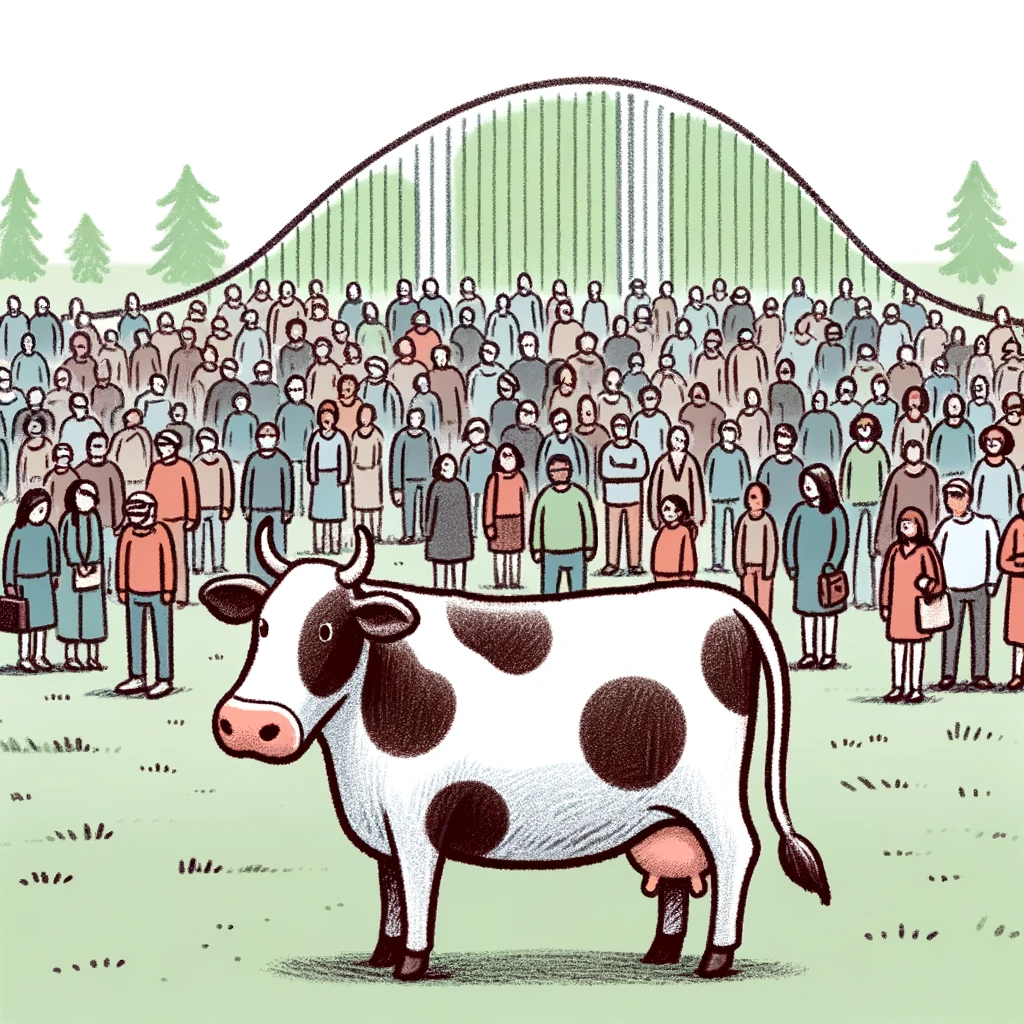
\includegraphics[width=0.5\textwidth]{figures/cow.png}
    \caption[The Wisdom of Crowds]{\textit{\textbf{The Wisdom of Crowds:}} The average of multiple noisy estimates of the weight of a cow is more accurate than any individual estimate. Created with the assistance of DALL·E 2}\label{fig:wisdomofcrowds}
\end{figure}

In this thesis, we will explore Canonical Correlation Analysis, a multiview learning method predicated on the assumption that different \gls{views} provide complementary information about latent variables. The following sections will establish a formal framework for representation learning and motivate the use of Canonical Correlation Analysis in harnessing complementary information from multiview data.

\section{Learning Representations: Definitions and Notation}

Suppose we have a sequence of vector-valued random variables $X\sps{i} \in \R^{D_i}$ for $i \in \{1, \dots, I \}$
We want to learn meaningful $K$-dimensional representations
\begin{equation}
    \label{eq:general-form-of-representations}
    Z\sps{i} = f\sps{i}( X\sps{i}; \theta\sps{i}).
\end{equation}
For convenience, define $D = \sum_{i=1}^I D_i$ and $\theta = \left(\theta\sps{i}\right)_{i=1}^I$.
Without loss of generality take $D_1 \geq D_2 \geq \cdots \geq D_I$.
We will consistently use the subscripts $i,j \in [I]$ for \gls{views};
$d \in [D_i]$ for dimensions of input variables;
and $l,k \in [K]$ for dimensions of representations - i.e. to subscript dimensions of $Z\sps{i}, f\sps{i}$.
Later on we will introduce total number of samples $N$.

In this report, when the functions $f$ are linear, we will typically refer to $u_k$ as \gls{weights}, $Z_k = X_k u_k$ as \gls{representations} or \gls{latent variables} (noting that in the CCA literature they are sometimes referred to as canonical variables \citep{borga_learning_1998}), depending on the context.
We will sometimes consider a matrix $U = \left(u_1, \dots, u_K\right) \in \R^{D \times K}$ of \gls{weights}, and a matrix $Z = \left(Z_1, \dots, Z_K\right) \in \R^{N \times K}$ of representations.
We will refer to the Pearson correlation between features and their respective latent variable $\Corr(X\sps{i}_j, Z_k)$ as the \gls{loadings} of $X\sps{i}_j$ on $Z_k$ \citep{rosipal2005overview, alpert1972interpretation, borga_learning_1998}, noting that the same concept has also been referred to as structure correlations \citep{meredith1964canonical}.

%Covariance matrices
We will use the notation $\Sigma_{ij}=\Cov(X\sps{i}, X\sps{j})$ for the population covariance matrix between the random variables associated with view $i$ and $j$. We will also use $\Sigma_{ii}= \Cov(X\sps{i})$ for the population covariance matrix of the random variables associated with view $i$ with each other.

\subsection{Generalized Eigenvalue Problems in linear algebra}
A Generalized Eigenvalue Problem (GEP) is defined by two symmetric matrices $A,B\in \mathbb{R}^{D\times D}$ \citep{stewart_matrix_1990}\footnote{more generally, $A,B$ can be Hermitian, but we are only interested in the real case}.
They are usually characterized by the set of solutions to the equation:
\begin{align}
    \label{eq:igep}
    Au=\lambda Bu
\end{align}
with $\lambda \in \R, u \in \R^D$, called (generalized) eigenvalue and (generalized) eigenvector respectively.
When $B$ is positive definite, then the GEP becomes equivalent to an eigen-decomposition of the symmetric matrix $B^\mhalf A B^\mhalf$ \citep{ghojogh2019eigenvalue}.
In addition, one can find a basis of eigenvectors spanning $\R^D$.
We define a top-$K$ subspace to be one spanned by some set of eigenvectors {$u_1,\dots,u_K$} with the top-$K$ associated eigenvalues $\lambda_1 \geq \dots \geq \lambda_K$.
We say a matrix $U \in \R^{D \times K}$ defines a top-$K$ subspace if its columns span one.

\paragraph{Uniqueness}
In GEPs, the eigenvectors $u$ are not in general unique, but the generalized eigenvalues $1 \geq \lambda_1 \geq \lambda_2 \geq \dots \geq 0$ are unique \citep{mills1988calculation}.

\subsection{Principal Components Analysis}

Principal Components Analysis \citep{hotelling1933analysis} (\acrshort{pca}) is a classical method in unsupervised machine learning for representation learning.
It is widely used for dimensionality reduction and feature extraction.
The primary goal of \acrshort{pca} is to transform the original high-dimensional data into a new coordinate system defined by orthogonal axes, capturing the most relevant aspects of the data.

In \acrshort{pca}, the representations are constrained to be linear transformations of the form:
\begin{equation}
    \label{eq:pca-linear-function-def}
    Z_k = X u_k,
\end{equation}
where $u_k$ are orthonormal basis vectors such that:
\begin{equation}
    \label{eq:pca-orthonormality-constraint}
    u_k^\top u_k = 1, \quad
    u_k^\top u_l = \delta_{kl} \text{ for } k \neq l.
\end{equation}

The primary goal of \acrshort{pca} is to maximize the variance of the representations \(Z_k\), finding the directions of maximal variance in the data.

\subsubsection{Optimization and Solution}
Mathematically, for the first principal component, this can be formulated as:

\begin{align}
    u_{\text{opt}} & = \underset{u}{\text{argmax}} \left( u^\top \Sigma u \right) \\
    \text{subject to:} \notag                                                     \\
    u^\top u       & = 1 \notag
\end{align}

Where \(\Sigma = \mathbb{E}[X^\top X]\) is the population covariance matrix of the single view data $X$.

The Lagrangian for this problem is:
\begin{equation}
    f(u,\lambda) = u^\top \Sigma u + \lambda(1 - u^\top u),
\end{equation}
where \(\lambda\) is the Lagrange multiplier.
Differentiating the Lagrangian yields the first-order conditions:
\begin{align}
    \Sigma u & = \lambda u, \\
    u^\top u & = 1.
\end{align}

\paragraph{Eigenvalue Problem}

This transforms the problem into an eigenvalue equation for the covariance matrix \(\Sigma\), which can be efficiently solved using standard libraries such as scikit-learn \citep{pedregosa2011scikit}.

The first principal component therefore corresponds to the eigenvector associated with the largest eigenvalue \(\lambda\).
Subsequent components are the remaining eigenvectors ordered by their corresponding eigenvalues.

\subsubsection{Limitations}
There are two major limitations of \acrshort{pca} that are relevant to this thesis.
The first is revealed by the epigraph of this chapter, which highlights the fact that \acrshort{pca} is not scale invariant.
This means that the principal components are sensitive to the scale of the data, and therefore the units in which the data is measured.
Furthermore, the interpretation of the principal components is challenging; they are linear combinations of all of the original features. For this reason, sparse variants of \acrshort{pca} have been developed \citep{zou2006sparse,zou2018selective}, which aim to find sparse linear combinations of the original features; interpretable as a subset of the original features contributing to a significant proportion of the variance in the data.
Another major limitation of \acrshort{pca} in the context of multiview learning is that it does not explicitly take advantage of either the redundancy or the complementary information in multiview data, even if we concatenate the views into a single random variable $X$.
Nevertheless, \acrshort{pca} remains a popular tool in practice \citep{greenacre2022principal} and is a useful baseline for multiview learning methods, and we will use it as a point of comparison throughout this thesis.

\subsection{Partial Least Squares}

Partial Least Squares (PLS) \citep{wold1975path} aims to maximize the shared covariance between two paired sets of data, referred to as \gls{views}. \acrshort{pls} can be seen as a generalization of \acrshort{pca}, where \acrshort{pca} becomes a special case when the two \gls{views} are identical.

\acrshort{pls} optimises for the dot product between the two views, a measure of similarity.

\begin{align}
    \label{eq:dot-product}
    \langle X\sps{1}u^{(1)}, X\sps{2}u^{(2)} =\sqrt{u\spsT{1}\Sigma_{11}u\sps{1}} \sqrt{u\spsT{2}\Sigma_{22}u\sps{2}} \cos(\theta)
\end{align}

Where $\theta$ is the angle between the two representations.
In order to constrain the problem, we set the norms of the weights to 1.

\subsubsection{Optimization and Solution}

The constrained optimization problem for \acrshort{pls} can therefore be formulated as:

\begin{align}
    u\sps{1}_{\text{opt}} & = \underset{u\sps{1}}{\mathrm{argmax}} \{ u\spsT{1} \Sigma_{12} u\sps{2} \} \\
    \text{subject to:} \notag                                                                             \\
    u\spsT{1}u\sps{1}   & = 1 \notag                                                                    \\
    u\spsT{2}u\sps{2}   & = 1 \notag
\end{align}

The Lagrangian for this optimization problem can be formulated as:

\begin{equation}
    f(u\sps{1}, \lambda) = u\spsT{1} \Sigma_{12} u\sps{2} + \lambda_1 (1 - u\spsT{1}u\sps{1}) + \lambda_2 (1 - u\spsT{2}u\sps{2})
\end{equation}

Upon deriving the first order conditions, we get:

\begin{align}
    \Sigma_{21} u\sps{1} & = \lambda_2 u\sps{2} \\
    \Sigma_{12} u\sps{2} & = \lambda_1 u\sps{1} \\
    u\spsT{1}u\sps{1}  & = 1                  \\
    u\spsT{2}u\sps{2}  & = 1
\end{align}

By substituting the constraint conditions into these equations, we find that \( \lambda_1 = \lambda_2 = \lambda \) by symmetry. Further simplification yields:

\begin{align}
    \Sigma_{21} \Sigma_{12} u\sps{2} & = \lambda^2 u\sps{2} \\
    \Sigma_{12} \Sigma_{21} u\sps{1} & = \lambda^2 u\sps{1}
\end{align}

\paragraph{Eigenvalue Problem}

Once again, we see that solving these equations will yield the \( u\sps{1} \) and \( u\sps{2} \) vectors as eigenvectors, this time of \( \Sigma_{12} \Sigma_{21} \) and \( \Sigma_{21} \Sigma_{12} \), respectively \citep{hoskuldsson1988pls}.

\paragraph{Generalized Eigenvalue Problem}

We can also represent the system of equations in matrix form as follows:

\begin{align}
    \begin{pmatrix}
        0           & \Sigma_{12} \\
        \Sigma_{21} & 0
    \end{pmatrix}
    \begin{pmatrix}
        u\sps{1} \\
        u\sps{2}
    \end{pmatrix}
    =
    \lambda
    I
    \begin{pmatrix}
        u\sps{1} \\
        u\sps{2}
    \end{pmatrix}
\end{align}

Which is of the form $A v = \lambda B v$. \acrshort{pls} is therefore also defined by the solution to a single generalized eigenvalue problem.

Given the notions of uniqueness in GEPs, the weights $u$ are not in general unique but we can write the vector of generalized eigenvalues $(\lambda_1, \dots, \lambda_K)$ representing covariances as:

\begin{align}
    \label{eq:pls-vector-of-correlations-def}
    \PLS_K(X^{(1)},X^{(2)}) \defeq (\lambda_k)_{k=1}^K
\end{align}

\subsubsection{Limitations} Like \acrshort{pca}, a major problem with applying \acrshort{pls} to neuroimaging and behavioural modalities is that \acrshort{pls} is not scale invariant.
This is because the dot product in equation~\ref{eq:dot-product} is not scale invariant since it is not normalized by the norms of the representations.
Since representations with larger norms will have larger dot products, \acrshort{pls} is biased towards larger representations.
It is therefore also biased towards the largest principal components in the data \citep{helmer2020stability}.
This is particularly problematic when there is a low signal to noise ratio since \acrshort{pls}.
Like \acrshort{pca}, another issue is the lack of sparsity in the \acrshort{pls} solution which has been an active area of research \citep{chun2010sparse, witten2009penalized}.

\subsection{Canonical Correlation Analysis}\label{sec:cca}

In Canonical Correlation Analysis (\acrshort{cca}), we aim to find the directions that maximize correlation, as opposed to maximizing covariance between two \gls{views} of a dataset.
This can be viewed as maximizing the cosine similarity between the two views, rather than the dot product, as in \acrshort{pls}.
Rearranging equation~\ref{eq:dot-product} yields:

\begin{align}
    \label{eq:cosine-similarity}
    \cos(\theta) = \frac{\langle X\sps{1}u^{(1)}, X\sps{2}u^{(2)}}{\sqrt{\langle X\sps{1}u^{(1)}, X\sps{1}u^{(1)}}\cdot \sqrt{\langle X\sps{2}u^{(2)}, X\sps{2}u^{(2)}}}= \frac{u\spsT{1}\Sigma_{12}u\sps{2}}{\sqrt{u\spsT{1}\Sigma_{11}u\sps{1}} \sqrt{u\spsT{2}\Sigma_{22}u\sps{2}}}
\end{align}

and we can see that the dot product from equation~\ref{eq:dot-product} is normalised by the inner products so that \acrshort{cca} is scale invariant, unlike \acrshort{pls}.
All that matters is the angle between the representations, not their magnitude.
Once again, in order to constrain the problem, we this time set the norms of the representations to 1.

\subsubsection{Optimization and Solution}
The optimization problem for \acrshort{cca} can be expressed as:

\begin{align}
    & u_{\text{opt}}=\underset{u}{\mathrm{argmax}}\{ u\spsT{1}X\spsT{1}X\sps{2}u\sps{2} \} \\
    & \text{subject to:} \notag                                                                \\
    & u\spsT{1}\Sigma_{11}u\sps{1}=1 \notag                                                  \\
    & u\spsT{2}\Sigma_{22}u\sps{2}=1 \notag
\end{align}

Although non-convex, numerous methods exist for solving the \acrshort{cca} problem, including eigendecomposition and generalized eigendecomposition solvers \citep{uurtio2017tutorial} and block coordinate descent via alternating least squares regressions \citep{golub1995canonical,sun2008least}.

The first-order conditions derived in the same manner as the \acrshort{pls} case are:

\begin{align}
    \label{CCA:FOCs}
    & \Sigma_{21}u\sps{1}=\lambda\sps{2} \Sigma_{22}u\sps{2} \\
    & \Sigma_{12}u\sps{2}=\lambda\sps{1} \Sigma_{11}u\sps{1} \\
    & u\spsT{1}\Sigma_{11}u\sps{1}=1                       \\
    & u\spsT{2}\Sigma_{22}u\sps{2}=1
\end{align}

\paragraph{Eigenvalue Problems}

Substituting the second two conditions into the first two, we get \(\lambda\sps{1}=\lambda\sps{2}=\lambda\). Finally, substituting the first two conditions into each other, we find the eigenvalue problems:

\begin{align}\label{eq:cca-eigenvalue-problems}
    & \Sigma_{11}^{-1}\Sigma_{12}\Sigma_{22}^{-1}\Sigma_{21}u\sps{1}=\lambda^2u\sps{1} \\
    & \Sigma_{22}^{-1}\Sigma_{21}\Sigma_{11}^{-1}\Sigma_{12}u\sps{2}=\lambda^2u\sps{2}
\end{align}

An alternative form of the \acrshort{cca} problem can be developed by reparameterizing \(u\sps{i*}=\Sigma_{ii}^{-\frac{1}{2}}u\sps{i}\). The optimization problem then becomes:

\begin{align}\label{eq:cca-reparameterized}
    & u_{\text{opt}}=\underset{u}{\mathrm{argmax}}\{ u\spsT{1}\Sigma_{11}^{-\frac{1}{2}}\Sigma_{12}\Sigma_{22}^{-\frac{1}{2}}u\sps{2} \} \\
    & \text{subject to:} \notag                                                                                                            \\
    & u\spsT{1}u\sps{1}=1 \notag                                                                                                         \\
    & u\spsT{2}u\sps{2}=1 \notag
\end{align}

This reparameterized form will later underpin Deep Canonical Correlation Analysis (\acrshort{dcca}) through the matrix $T=\Sigma_{11}^{-\frac{1}{2}}\Sigma_{12}\Sigma_{22}^{-\frac{1}{2}}$.
This form also shows that \acrshort{pls} and \acrshort{cca} can be made equivalent by whitening the data matrices before constructing the covariance matrix.
When the number of features exceeds the number of samples (\(p>n\)), \acrshort{cca} becomes degenerate because the within-view covariance matrices cannot be inverted—contrasting with \acrshort{pls}, which is always computable.

\paragraph{Generalized Eigenvalue Problem}

We can also represent the system of equations in equation~\ref{CCA:FOCs} as a matrix equation:

\begin{align}
    \begin{pmatrix}
        0           & \Sigma_{12} \\
        \Sigma_{21} & 0
    \end{pmatrix}
    \begin{pmatrix}
        u\sps{1} \\
        u\sps{2}
    \end{pmatrix}
    =
    \lambda
    \begin{pmatrix}
        \Sigma_{11} & 0           \\
        0           & \Sigma_{22}
    \end{pmatrix}
    \begin{pmatrix}
        u\sps{1} \\
        u\sps{2}
    \end{pmatrix}
\end{align}

Which is once again of the form $A u = \lambda B u$. \acrshort{cca}, like \acrshort{pls}, is therefore also defined by the solution to a single generalized eigenvalue problem.

\paragraph{Canonical Correlations}
In the case of \acrshort{cca}, the generalized eigenvalues $\lambda$ are generally called canonical correlations \citep{hotelling1935canonical, hotelling1992relations}.
Given the notions of uniqueness in GEPs, the weights $u$ are not in general unique but we can write the vector of generalized eigenvalues or canonical correlations as:
\begin{align}
    \label{eq:cca-vector-of-correlations-def}\small
    \CCA_K(X^{(1)},X^{(2)}) \defeq (\rho_k)_{k=1}^K
\end{align}

\subsubsection{Limitations}

A major limitation of \acrshort{cca} is revealed by the forms in equations \ref{eq:cca-eigenvalue-problems} and equation~\ref{eq:cca-reparameterized}; \acrshort{cca} in general requires the inversion of covariance matrices, which is computationally expensive, potentially numerically unstable, and impossible when the number of features exceeds the number of samples such that the covariance matrices are not full rank.

\subsection{Multiview \acrshort{cca}}

Multiview \acrshort{cca} or \acrshort{mcca} is a straightforward extension of \acrshort{cca} to the case of 3-or more datasets.
The goal is to find a set of directions \(u\sps{i}\) such that the pairwise correlations between the views are maximized.

\subsubsection{Optimization and Solution}

The optimization problem for \acrshort{mcca} can be stated as:
\begin{align}
    & u_{\text{opt}} = \underset{u}{\mathrm{argmax}} \sum_{i=1}^{m} \sum_{j=1, j \neq i}^{m} u\spsT{i} \Sigma_{ij} u\sps{j} \\
    & \text{subject to:} \notag                                                                                               \\
    & \sum_{i=1}^{m} u\spsT{i} \Sigma_{ii} u\sps{i} = 1 \notag
\end{align}

\paragraph{Generalized Eigenvalue Problem}

The generalized eigenvalue problem (GEP) for MCCA can be written in matrix form as follows:

\begin{align}
    \small
    \begin{pmatrix}
        0           & \Sigma_{12} & \cdots & \Sigma_{1m} \\
        \Sigma_{21} & 0           & \cdots & \Sigma_{2m} \\
        \vdots      & \vdots      & \ddots & \vdots      \\
        \Sigma_{m1} & \Sigma_{m2} & \cdots & 0
    \end{pmatrix}
    \begin{pmatrix}
        u\sps{1} \\
        u\sps{2} \\
        \vdots   \\
        u\sps{m}
    \end{pmatrix}.
    =
    \lambda
    \begin{pmatrix}
        \Sigma_{11} & 0           & \cdots & 0           \\
        0           & \Sigma_{22} & \cdots & 0           \\
        \vdots      & \vdots      & \ddots & \vdots      \\
        0           & 0           & \cdots & \Sigma_{mm}
    \end{pmatrix}
    \begin{pmatrix}
        u\sps{1} \\
        u\sps{2} \\
        \vdots   \\
        u\sps{m}
    \end{pmatrix}.
\end{align}

This GEP formulation of MCCA can be presented in a unified framework generalizing CCA and ridge-regularized extensions. Indeed, we now take $A,B_\alpha \in \R^{D \times D}$ to be block matrices $A = (A\sps{ij})_{i,j=1}^I, B_\alpha = (B_\alpha\sps{ij})_{i,j=1}^I$ where the diagonal blocks of $A$ are zero, the off-diagonal blocks of $B_\alpha$ are zero, and the remaining blocks are defined by:
\begin{align}
    \label{eq:gep-most-general-formulation}%\small
    A^{(ij)} &= \Cov(X\sps{i}, X\sps{j}) \text{ for } i \neq j, \quad % \text{ for } i,j \in [I], ; \:\:
    B_\alpha^{(ii)} = \alpha_i I_{D\sps{i}} + (1-\alpha_i) \Var(X\sps{i})  %\text{ for } i \in [I]
\end{align}
Where $\alpha \in [0,1]^I$ is a vector of ridge penalty parameters: taking $\alpha_i = 0 \: \forall i$ recovers CCA and $\alpha = 1 \: \forall i$ recovers PLS.
We may omit the subscript $\alpha$ when $\alpha=0$ and we recover the `pure CCA' setting; in this case, following \ref{eq:cca-vector-of-correlations-def} we can define

\begin{align}
    \MCCA_K(X\sps{1},\dots,X\sps{I})
\end{align}

to be the vector of the top-$K$ generalized eigenvalues which are the average of the top-$K$ correlations between each pair of views.

\subsection{Linear Discriminant Analysis LDA}

Linear Discriminant Analysis (LDA) can be viewed as a special case of Canonical Correlation Analysis (CCA) where \(X^{(2)}\) is a one-hot encoded matrix representing the class labels.
This allows us to draw a connection between the unsupervised learning framework of \acrshort{cca} and the supervised framework of LDA\citep{balakrishnama1998linear,riffenburgh1957linear}, thus expanding the understanding of both algorithms.

\textbf{Intuition:} In LDA, the aim is to find a lower-dimensional subspace where the classes are maximally separated. This objective can be viewed through the lens of \acrshort{cca}, where the optimal directions \(u^{(1)}\) and \(u^{(2)}\) in the original and one-hot encoded spaces aim to maximize correlation. In the LDA context, \(u^{(1)}\) would maximize the separation between classes.

\subsubsection{Optimization and Solution}

Mathematically, LDA is reduced to solving a generalized eigenvalue problem involving the between-class scatter matrix \(S_B\) and the within-class scatter matrix \(S_W\):

\[
    \hat{S_B} = \sum_{i=1}^{c} n_i (\mu_i - \mu)(\mu_i - \mu)\top
\]

\[
    \hat{S_W} = \sum_{i=1}^{c} \sum_{x \in X_i} (x - \mu_i)(x - \mu_i)\top
\]

\textbf{Connection to \acrshort{cca}:} When \(X^{(2)}\) is the one-hot encoded matrix of class labels, the \acrshort{cca} problem effectively tries to maximize the correlation between the feature vectors and their corresponding labels.
This turns out to be equivalent to maximizing the between-class variance in LDA while minimizing the within-class variance.
Thus, LDA can be thought of as a constrained form of \acrshort{cca}, tailored to classification tasks.

This perspective unifies the two algorithms and shows that the core objective—finding meaningful relationships or directions in the data—is shared between both \acrshort{cca} and LDA.

\subsection{Sample Covariance and Population Covariance}
In the previous sections, the methods were described in terms of population covariance matrices such as \(\Sigma_{11}=\mathbb{E}[X\spsT{1} X\sps{1}]\), \(\Sigma_{22}=\mathbb{E}[X\spsT{2} X\sps{2}]\), and \(\Sigma_{12}=\mathbb{E}[X\spsT{1} X\sps{2}]\).
These population covariances assume an underlying probability distribution from which the data are drawn.

\textbf{Sample Covariance:} In practical settings, we often do not have access to the entire population but only to a sample. Hence, we can use the Sample Average Approximation to estimate these covariances:

\[
    \hat{\Sigma}\sps{12} = \frac{1}{b-1} \bar{\mathbf{X}\sps{1}} \bar{\mathbf{X}\sps{2}}\top
\]

Here, \(b\) denotes the size of the minibatch, and \(\mathbf{X}\sps{1} \in \mathbb{R}^{p \times b}\) and \(\mathbf{X}\sps{2} \in \mathbb{R}^{q \times b}\) are the data matrices for the samples from \(X\sps{1}\) and \(X\sps{2}\), respectively. The bar over \(\mathbf{X}\sps{1}\) and \(\mathbf{X}\sps{2}\) signifies that these are centered versions of the matrices, i.e., the mean has been subtracted from each column.
For the ease of both reader and writer, we will drop the bars for the remainder of the thesis and assume that the data are always centered without loss of generality.

\textbf{Practical Implications:} Using sample covariance matrices introduces some estimation error but allows us to apply the methods in real-world scenarios where population-level data are unattainable.
Additionally, the use of minibatches (chunks of data) in later chapters provides a computationally efficient way to estimate these covariances in large-scale problems, at the cost of some additional statistical noise.

\textbf{Connection to Previous Methods:} The use of sample covariance matrices is directly applicable to algorithms like \acrshort{cca} and LDA. When replacing the population covariances \(\Sigma\sps{ij}\) with sample estimates, the optimization problems remain structurally similar but are solved using the sample data.

This dual perspective—considering both population and sample covariance matrices—enables a more robust and flexible approach to the methods discussed, bridging the gap between theoretical analysis and practical application.
It will be particularly useful in the context of chapter \ref{ch:loadings} where we will use population variables as ground truth while estimating the models using sample data.


\section{Practical Frameworks for Evaluating Multiview Learning Methods}

At this point, we have introduced the theoretical foundations of multiview learning, and a number of classical representation learning algorithms including \acrshort{cca} and its variants.
However, it is not yet clear how we should evaluate these methods in practice.
In this section, we compare the machine learning and the statistical approach of permutation testing.
These two approaches are not mutually exclusive, and statistical learning theory has emerged as a unifying framework for both perspectives \citep{vapnik1999nature, hastie2009elements}.

\subsubsection{Permutation Testing}

\begin{figure}
    \centering
    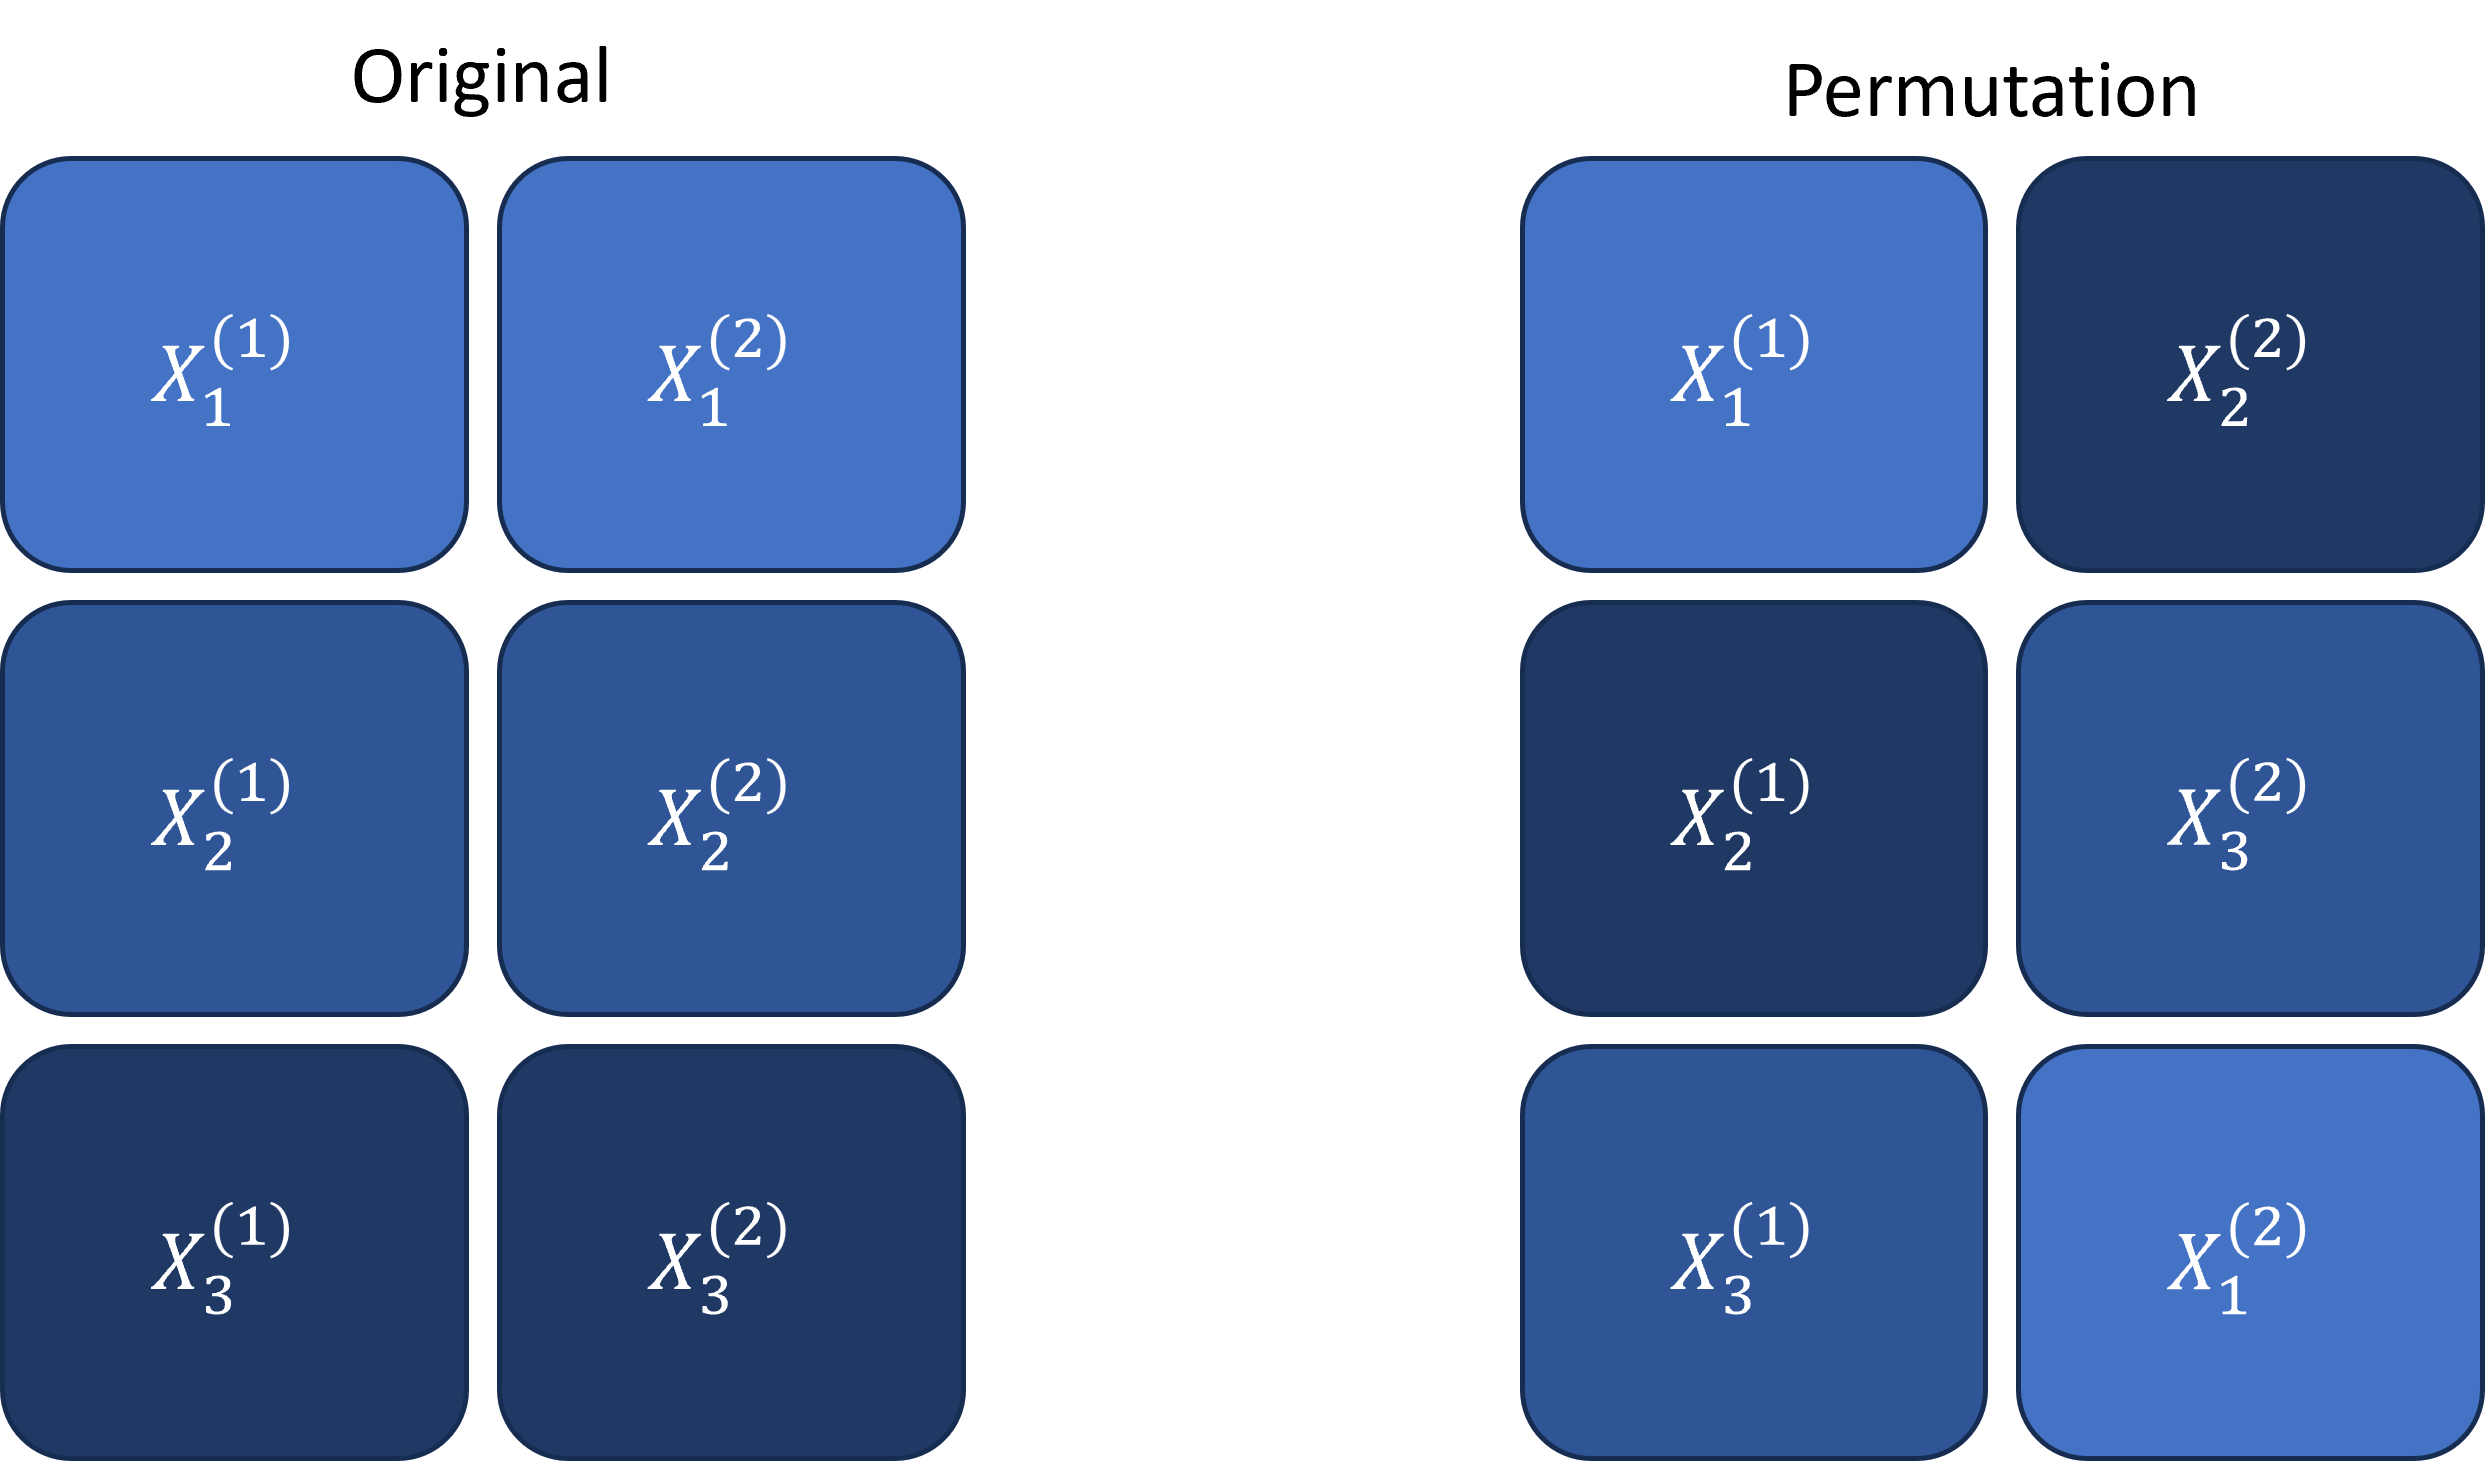
\includegraphics[width=0.8\textwidth]{figures/permutation_test.png}
    \caption{Schematic of the permutation testing procedure. The original data are randomly shuffled, and the model is retrained on the shuffled data. This process is repeated multiple times, and the model's performance on the original data is compared to the distribution of performances on the shuffled data.}
    \label{fig:statistical-inference}
\end{figure}

Permutation testing offers a robust way to evaluate the significance of the results obtained by multiview learning methods and, for a single component, is a relatively simple process \citep{winkler2020permutation}.
As illustrated in Figure~\ref{fig:statistical-inference}, the views are randomly and separately shuffled, and the model is then trained and tested on this permuted data.
This process is repeated multiple times, generating a distribution of performance metrics under the null hypothesis, where there is no relationship between the views.
The actual performance of the model on the unshuffled data is then compared to this distribution.
If the actual performance is significantly better than the permuted performance, it suggests that the model is capturing meaningful relationships in the data.

\subsubsection{Machine Learning}

\begin{figure}
    \centering
    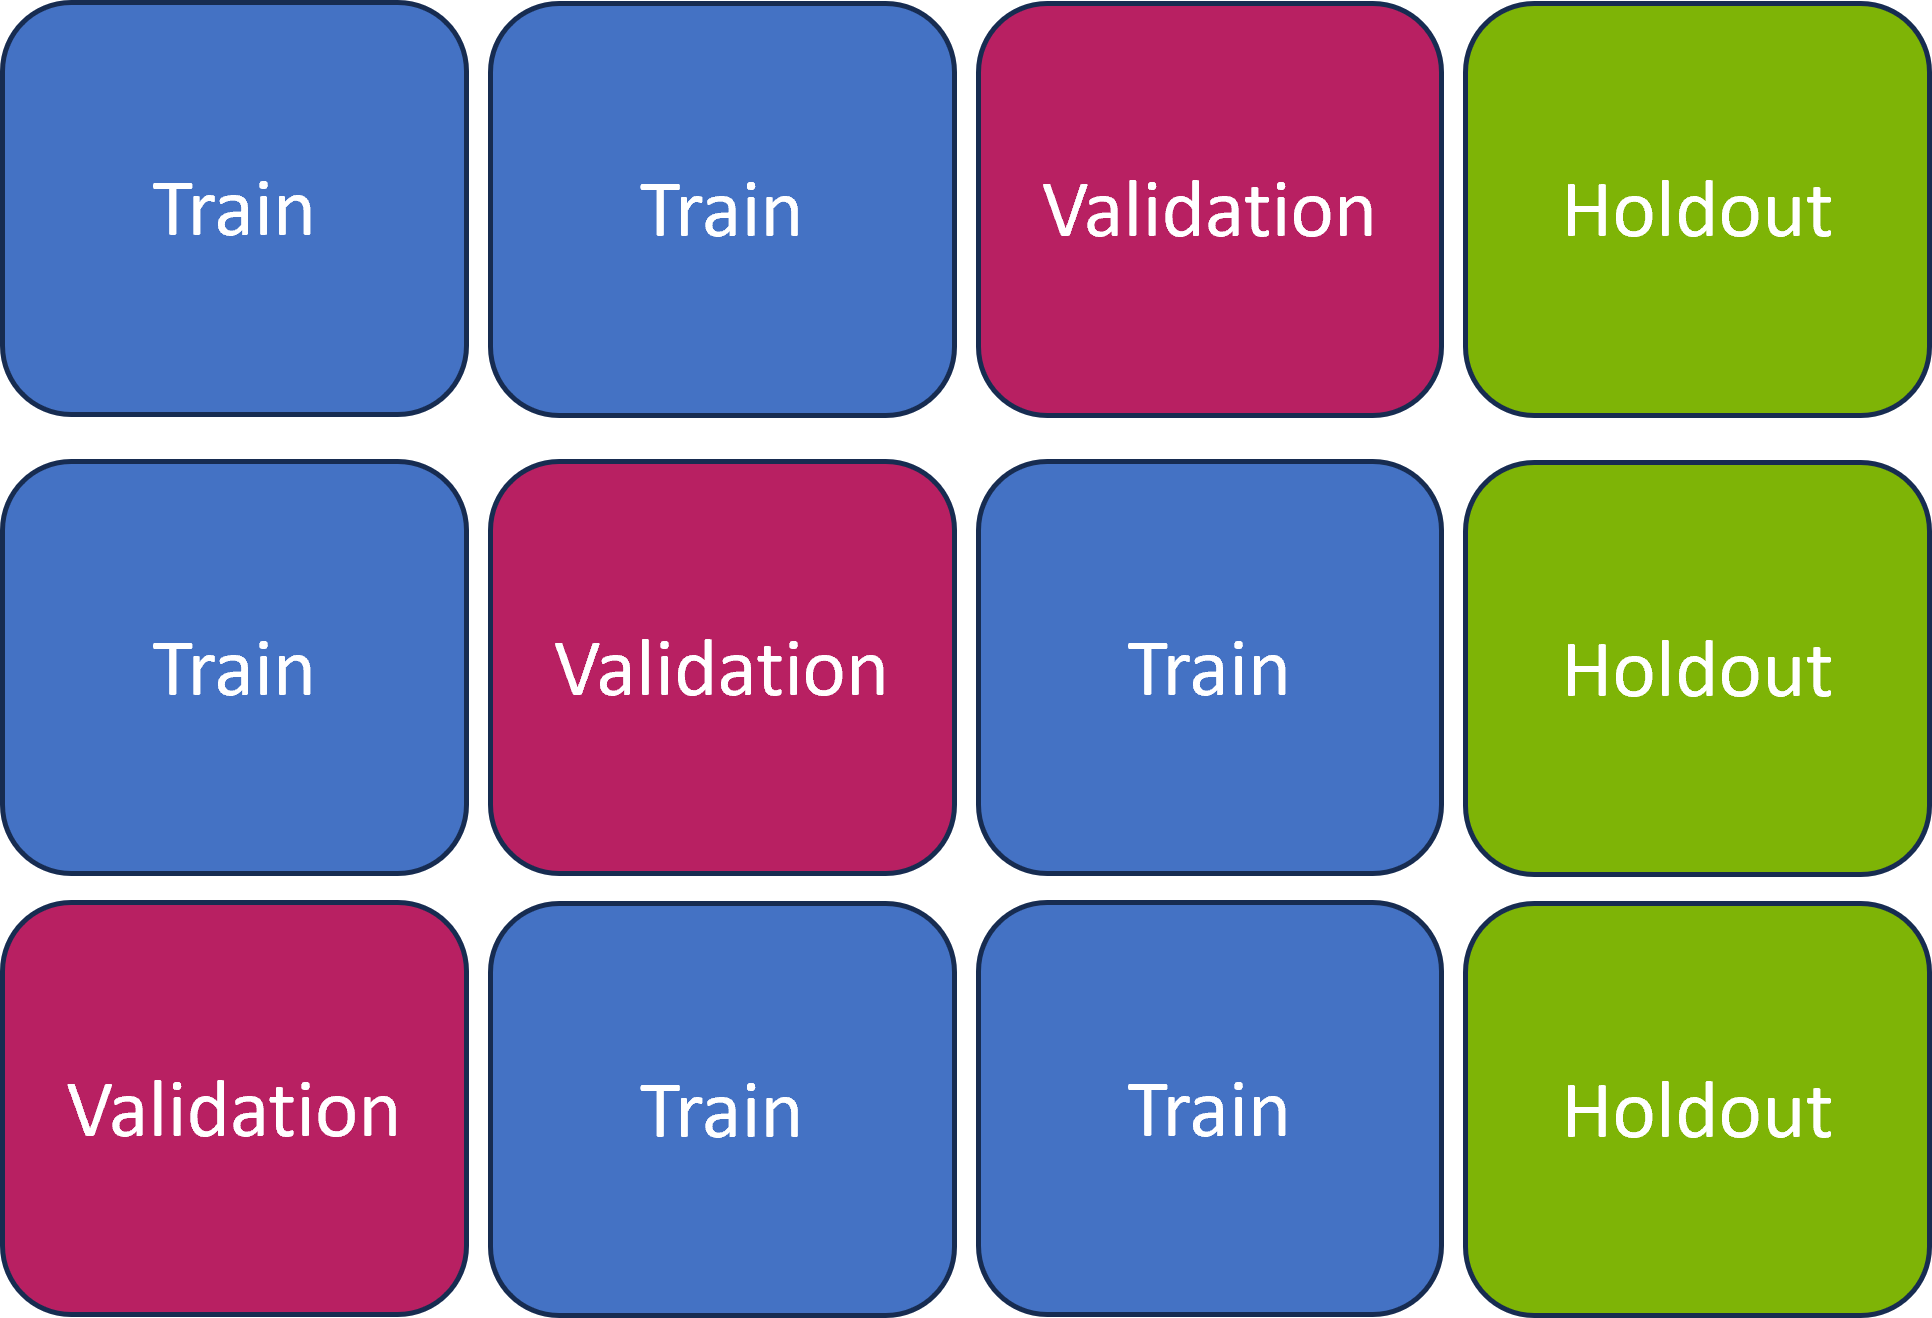
\includegraphics[width=0.8\textwidth]{figures/cross-validation.png}
    \caption{Schematic of the cross-validation procedure. The original data are partitioned into training and test sets. In cross-validation, the training set is further partitioned into training and validation sets. The model is trained on the training set and evaluated on the validation set for different parameter values. The parameter value with the best performance on the validation set is selected, and the model is retrained on the entire training set. The final model is evaluated on the single test or holdout set.}
    \label{fig:machine-learning}
\end{figure}

The machine learning approach to evaluating multiview learning methods is to use a holdout or test set to estimate the out-of-sample performance of the model.
Within the training set, where necessary, cross-validation is used to select the best model hyperparameters.
Cross-validation involves partitioning the training set into training and validation sets, training the model on the training set, and evaluating the model on the validation set.
When this is performed for multiple subsets of the training set, it is referred to as \(k\)-fold cross-validation as illustrated in figure \ref{fig:machine-learning}.
The model hyperparameters are then selected based on the performance across the validation sets.
The model is then retrained on the entire training set using the best hyperparameters, and evaluated on the test set.

In this thesis, we will use the machine learning approach throughout.
This is because in scaling up to large datasets, permutation testing becomes computationally intractable.
This is because permutation testing requires retraining the model multiple times on the permuted data.
This comes at the cost of only being able to evaluate models with a point estimate of performance, rather than a distribution.
In chapter \ref{ch:loadings}, we observe and argue that signals of interest have a large effect size, and therefore permutation testing is not necessary to evaluate the significance of the results.

\subsection{Components and Subspaces in CCA}

\subsubsection{Eigenvalue Problems in CCA}

While our focus so far has primarily been on the top-1 eigenvector-eigenvalue pair, it's important to note that the methodology also extends to the top-k subspace problem. This broader approach involves identifying the top-k eigenvectors and their corresponding eigenvalues.

\subsubsection{Addressing the Top-k Problem}

Transitioning from a focus on the top-1 component to exploring the top-k subspace introduces additional complexities. One common method to solve the top-k problem is to identify the top-1 component and then apply a deflation process to find subsequent orthogonal components.
Deflation involves removing the top-1 component from the data and then repeating the process to find the next top-1 component. This process is repeated until the desired number of components is found.
For instance, Hotelling's Deflation \citep{hotelling1933analysis} involves removing the top-1 component from the data, while Projection Deflation \citep{mackey2008deflation} involves projecting the data onto the orthogonal complement of the top-1 component.
Different deflation methods enforce different forms of orthogonality, which can impact the resulting components and their interpretation, particularly when the first component is not a true eigenvector.

\subsubsection{Non-Uniqueness of Components}

Furthermore, non-uniqueness is a significant challenge in representation learning, particularly when eigenvectors have repeated eigenvalues. Imagine a scenario where the top-1 eigenvalue is repeated \(k\) times. In this case, there are \(k\) possible eigenvectors that can be associated with the top-1 eigenvalue. While this is unlikely to occur in practice, the eigenvalues can in practice be very close to each other, leading to numerical instability and non-uniqueness in the components. Particularly true in cross-validation settings, this non-uniqueness can lead to instability in the components, complicating their interpretation and comparison.
For example, the top-1 component in one analysis might be the second component in another analysis, making it difficult to compare the results.

This non-uniqueness also has a grounding in the probabilistic perspectives on PCA and CCA (introduced in chapter \ref{ch:loadings}), where the latent variables are considered unique only up to a rotation.
This perspective further reinforces the subspace approach, emphasizing the identification of a subspace rather than specific directions within it.

\paragraph{Thesis Approach: Concentrating on the Top-1 Component}

In this thesis, we focus on the top-1 component in CCA to align with and facilitate comparison with typical componentwise studies in brain-behavior research.
This choice is driven by the complexity associated with the top-k problem and the variety of methods available to address it.
Under the assumption of a significant eigengap\footnote{An `eigengap' refers to the difference in magnitude between consecutive eigenvalues in an eigenvalue problem. A significant eigengap between the first and second eigenvalues suggests that the first eigenvalue (and its corresponding eigenvector) is distinctly more significant than the next, lending credence to its uniqueness and importance.}, the first component can be considered equivalent to the top-1 subspace.
This equivalence allows for a clear and interpretable analysis, making the top-1 subspace a straightforward and reliable choice for studying multivariate data.
It is important to note that while we focus on the top-1 component, the later sections of the thesis introduce a method for simultaneously solving the complete subspace, addressing broader subspace analyses.


\section{Multiview Learning in Neuroimaging}

Finally, we review important applications of multiview learning from the literature in neuroimaging, which will be our reference in chapters \ref{ch:als} and \ref{ch:loadings}.

\subsection{Multiview Data in Neuroscience and Genetics}

In neuroscience and genetics, two specific types of multiview studies are particularly relevant to this thesis: brain-behavior studies and imaging-genetics.
Both involve the integration of data from multiple sources, offering rich insights into complex phenomena.

Brain-behavior studies typically involve pairing neuroimaging data, such as that obtained from Structural MRI (sMRI) or Functional MRI (fMRI), with non-imaging data like responses from questionnaires, cognitive test results, and other behavioral assessments.
sMRI provides detailed anatomical brain images, essential for understanding brain structure and neurological disorders \citep{kanai2011structural}, while fMRI focuses on brain function by mapping activity during cognitive tasks \citep{miranda2021systematic}.
The integration of these imaging techniques with behavioral data offers a comprehensive view of how brain structures and functions correlate with behavioral and cognitive patterns \citep{rypma2001age,genon2022linking}.

Imaging-Genetics, another critical multiview approach, combines neuroimaging data with genetics and omics information \citep{le2008sparse}.
This interdisciplinary field seeks to understand the genetic influences on brain structure and function, thereby illuminating the genetic basis of neuropsychiatric disorders and cognitive traits \citep{bogdan2017imaging}.
Studies in this area can explore how specific genetic variations correlate with differences in brain morphology or activity patterns observed in neuroimaging \citep{liu2014review}.

Together, these multiview approaches are fundamental in advancing our understanding of the brain's structure, function, and its interactions with genetic and behavioral factors.
They represent key applications of SSL in neuroscience and genetics, providing comprehensive insights that underpin developments in these fields.

\subsection{Applications of Multiview Learning in Neuroimaging}

There have been a number of applications of \acrshort{cca} and related methods to multiview problems in neuroimaging.
Using resting state fMRI data, modes of correlation have been found that relate to differences in sex and age relating to drug and alcohol abuse, depression and self harm \citep{mihalik2019brain}.
A similar mode relating to `positive-negative' wellbeing has been found across studies \citep{smith2015positive} suggesting that mental wellbeing has a relationship (though not necessarily causally) with functional connectivity between networks in the brain.
Later in this dissertation we will replicate and build on the findings from this paper by using regularised and non-linear \acrshort{cca} methods.
Owing to the high dimensionality of neuroimaging data, regularisation has been a particular focus of multiview learning in neuroimaging. \citet{mihalik2022canonical} reviews the application of \acrshort{cca} to neuroimaging data and highlights the importance of regularisation in this context. \citet{bilenko2016pyrcca} 
CCA has also been used as a preprocessing step in order to identify groups of subjects in the latent variable space.

In particular, \acrshort{cca} and clustering have been used to identify depression using fMRI data \citep{dinga2019evaluating,drysdale2017resting}.
CCA has also been used in the manner we described to denoise two \gls{views} of a dataset such as separate measures of neuroimaging data \citep{zhuang2020technical} to remove artefacts.
Deep \acrshort{cca} has recently been used to extract features for the diagnosis of schizophrenia\citep{qi2016deep}.

%\section{Open challenges in Multiview Learning and CCA}
%
%This thesis has been motivated by a number of open challenges in multiview learning and canonical correlation analysis.
%Chapter \ref{ch:als} and \ref{ch:loadings} will address the first challenge, which is the regularisation of \acrshort{cca} in high dimensional settings and the interpretation of the resulting components.
%Chapters \ref{ch:gradient_descent}, \ref{ch:deep_learning}, and \ref{ch:software} will address the second challenge, the efficient application of \acrshort{cca} to big data.
%Finally \ref{ch:deep_learning} will also address the third challenge, extending \acrshort{cca} to Deep Self-Supervised Learning.
%
%\subsection{Interpretability and Regularization}
%
%\textcolor{red}{TODO: Add a paragraph on interpretability and regularization}
%
%\subsection{Efficient Algorithms for High-Dimensional Data}
%
%\textcolor{red}{TODO: Add a paragraph on efficient algorithms for high-dimensional data}
%
%\subsection{Non-linear \acrshort{cca} and Joint Embedding Self-Supervised Learning}
%
%\textcolor{red}{TODO: Add a paragraph on non-linear \acrshort{cca} and Joint Embedding Self-Supervised Learning}
%
%






% %
\graphicspath{{chapters/regularization}}
\chapter{Regularization of CCA Models to add Structure}\label{chap:als}
\minitoc
% chktex-file 44 
% chktex-file 3

\epigraph{The essence of strategy is choosing what not to do.}{\textit{Michael E. Porter}}
\section{Introduction}\label{sec:introduction}

This chapter explores the role of regularization in improving the performance and interpretation of Canonical
Correlation Analysis (CCA) using data from the Human Connectome Project (HCP) and Alzheimer's Disease Neuroimaging Initiative (ADNI) datasets.

CCA models often exhibit shortcomings when dealing with high-dimensional data.
This challenge is particularly acute in brain-behavior studies.
In these studies, neuroimaging modalities typically have a much higher dimensionality than the available sample size.
In this context, CCA models are prone to overfitting, leading to spurious correlations and poor generalization.
Regularization, having been extensively studied and well-understood in the contexts of Linear Regression and Inverse Problems, introduces a deliberate bias to guide models towards more generalizable solutions.
This principle, when applied to CCA, offers a promising avenue for addressing its challenges, ensuring that the model does not overfit to the noise in the data but captures the true underlying patterns.
Furthermore, regularization can help us improve the interpretability of the results most clearly by encouraging sparsity.

With this perspective in mind, we propose a flexible regularized alternating least squares (FRALS) framework for CCA which allows us to incorporate any regularized least squares solver to efficiently implement a wide range of regularization functions, but in particular allows us to efficiently implement the elastic net penalty with controllable L2 and L1 penalties so that we can control the bias towards the largest principal components while still encouraging sparsity in the weights.
This is in contrast to much of the previous work on sparse Brain-Behavior analysis which has used a PLS objective with lasso constraints (SPLS), which inherits a bias towards the largest principal components from PLS.

We apply FRALS with ElasticNet regularization to the Human Connectome Project (HCP) dataset, and show that it outperforms other CCA models in terms of out-of-sample canonical correlation.
We also show that the identified mode of variation is distinct from previous work which identified latent variables with loadings related to cognitive tests and negatively related to cigarette, tobacco or alcohol\citep{smith2015positive}.
FRALS has stronger correlations with the Line Orientation test, which measures visuospatial abilities, and the parietal lobe, which is known to be involved in visuospatial processing.
This further demonstrates the importance of matching the model to the data generation process with the appropriate regularization.

This chapter expands on my work previously showcased at the OHBM conference and draws connections to a tutorial paper I co-authored, where I contributed a number of simulations\citep{mihalik2022canonical}.

\section{Background: Regularization for High-Dimensional and Structured Data}\label{sec:background}

Like Linear Regression, Canonical Correlation Analysis does not have a unique solution when the number of features exceeds the number of observations in either view.
More generally, as the number of features increases, the number of parameters in the model increases, and the model becomes more prone to overfitting particularly when the signal-to-noise ratio is low.
Furthermore, when features are correlated, the estimates of the parameters become unstable.
Most obviously, if two features are perfectly correlated, the model is not identifiable (has no unique solution) because we can swap the weights between the two features without changing the model.
Regularization is a powerful tool for addressing these problems, and has been widely used in Linear Regression and Inverse Problems.
Moreover, regularization can help us improve the interpretability of the results by encouraging sparsity in the weights and/or loadings.

\subsubsection{Shrinkage Regularization}

Shrinkage regularization is an effective method for improving the performance of linear models in high-dimensional settings.
Shrinkage methods bias models towards lower variance solutions by shrinking the model parameters (weights) towards zero.
Shrinkage regularization works on the premise that, generally, larger principal components are more likely to represent meaningful data patterns rather than noise.

\paragraph{PLS as Shrinkage Regularization}

PLS can be interpreted as a form of shrinkage regularization applied to CCA. We can explain this by considering an analogy between CCA and Linear Regression (indeed Linear Regression is a special case of CCA where \(X^{(2)}\) has one feature).

In Linear Regression, the ridge regression solution is given by:
\begin{align}
    \hat{\beta}_{\text{ridge}} = ((1-c)\Sigma_{X,X} + c I)^{-1} \Sigma_{X,y}
\end{align}
Where \(c\) is the regularization parameter between 0 and 1\footnote{It is more common to see $(\Sigma_{X,X} + c I)^{-1} \Sigma_{X,y}$ but these are equivalent up to a scalar factor and this form helps us later on}.
The ridge penalty acts in two important ways:
\begin{itemize}
    \item It shrinks the weights towards zero.
    \item It biases the solution to high covariance directions rather than high correlation directions.
\end{itemize}

As $c$ becomes large, $\lim_{c \to \infty} (\Sigma_{X,X} + c I)^{-1} = (c I)^{-1}$
, so that $\hat{\beta}_{\text{ridge}}=\frac{\Sigma_{X,y}}{c}$, which is precisely the covariance of the features of $X$ with $Y$ scaled by $c$ (and shrunk towards zero for $c \geq 1$).
Notice that the ridge regression solution is no longer sensitive to the correlation of features in $X$.
Additionally, notice that for sufficiently large $c$, $(\Sigma_{X,X} + c I)$ is invertible even if $\Sigma_{X,X}$ is not invertible, so that ridge regression can be well defined even when the number of features exceeds the number of observations.

Now consider the CCA problem.
Firstly, recall that PLS and CCA are equivalent up to a scaling when the covariance matrices are identity matrices, a similar relationship to the relationship between Linear and Ridge Regression.
Consider the well-known form of CCA given in equation~\ref{eq:cca}\citep{mihalik2022canonical} (formed by reparameterizing \(u\sps{i}=(\Sigma_{ii})^{-\frac{1}{2}}u\sps{i}\)):

\begin{align}\label{eq:cca}
     & u_{\text{opt}}=\underset{u}{\mathrm{argmax}}\{ u\spstop{1}(\Sigma_{11}+ c I)^{-\frac{1}{2}}\Sigma_{12}(\Sigma_{22}+c I)^{-\frac{1}{2}}u\sps{2} \} \\
     & \text{subject to:} \notag \\
     & u\spstop{1}u\sps{1}=1, u\spstop{2}u\sps{2}=1 \notag
\end{align}

As we increase $c$, $\lim_{c \to \infty} (\Sigma_{ii}+ c I)^{-\frac{1}{2}}= (c I)^{-1}$ so that the objective approaches:

\begin{align}
     & u_{\text{opt}}=\underset{u}{\mathrm{argmax}}\{ u\spstop{1}(c I)^{-1}\Sigma_{12}(c I)^{-1}u\sps{2} \} \\
        & \text{subject to:} \notag \\
        & u\spstop{1}u\sps{1}=1, u\spstop{2}u\sps{1}=1 \notag
\end{align}

Which is precisely the PLS objective and constraints with an arbitrary scaling of the covariance matrix $\Sigma_{12}$ by $\frac{1}{c^2}$.
For this reason, we can consider PLS as a shrinkage method for CCA equivalent to adding a very large ridge regularization.
This has two important consequences.
Fortunately, it is well defined even when the number of features exceeds the number of observations so we can always apply PLS to high-dimensional data.
Unfortunately, it biases the solution towards the largest principal components.
PLS is evidently not a nuanced as a tool for regularization because it offers no control over the degree of regularization applied.
Just as one would rarely resort to maximally regularized ridge regression except in extremely low sample sizes, one should be cautious about using PLS to identifying mutually correlated latent variables.

\paragraph{Ridge Regularization}

For this reason,~\cite{vinod1976canonical} proposed the `Canonical Ridge' which combined the PLS and CCA constraints in a single constrained optimization:

\begin{align}
     & u\sps{1}_{\text{opt}} = \underset{u\sps{1}}{\mathrm{argmax}} \{ u\spstop{1} \hat{\Sigma_{12}} u\sps{2} \} \\
     & \text{subject to:} \notag \\
     & (1 - c_1) u\spstop{1} \hat{\Sigma_{11}} u\sps{1} + c_1 u\spstop{1} u\sps{1} = 1 \notag \\
     & (1 - \tau_2) u\spstop{2} \hat{\Sigma_{22}} u\sps{2} + \tau_2 u\spstop{2} u\sps{2} = 1 \notag
\end{align}

Where $c_1$ and $\tau_2$ are the ridge regularization parameters for the first and second views respectively.

\paragraph{PCA-CCA} PCA can be used as a regularization method for CCA by using only the first \( k \) principal components of each view as the input to CCA.
This reduces the dimensionality of the data and can help to avoid overfitting.
However, it also risks overlooking subtle but crucial relationships between variables, as it focuses on leading principal components.

While PCA-CCA and rCCA are effective for finding signal in the presence of noise, they do not produce sparse
solutions and so do not clearly lend themselves to interpretation.

\paragraph{Visual Comparison of Shrinkage Techniques}

The distinct effects of Ridge and PCA on the eigenvalues of the effective covariance matrices can be clearly visualized.
As shown in Figure~\ref{fig:shrinkage}, Ridge regularization uniformly reduces the magnitude of all principal components towards zero, with a proportionally greater effect on the smaller components.
On the other hand, PCA-CCA, by focusing on leading principal components, only shrinks the smallest ones.

\begin{figure}
    \centering
    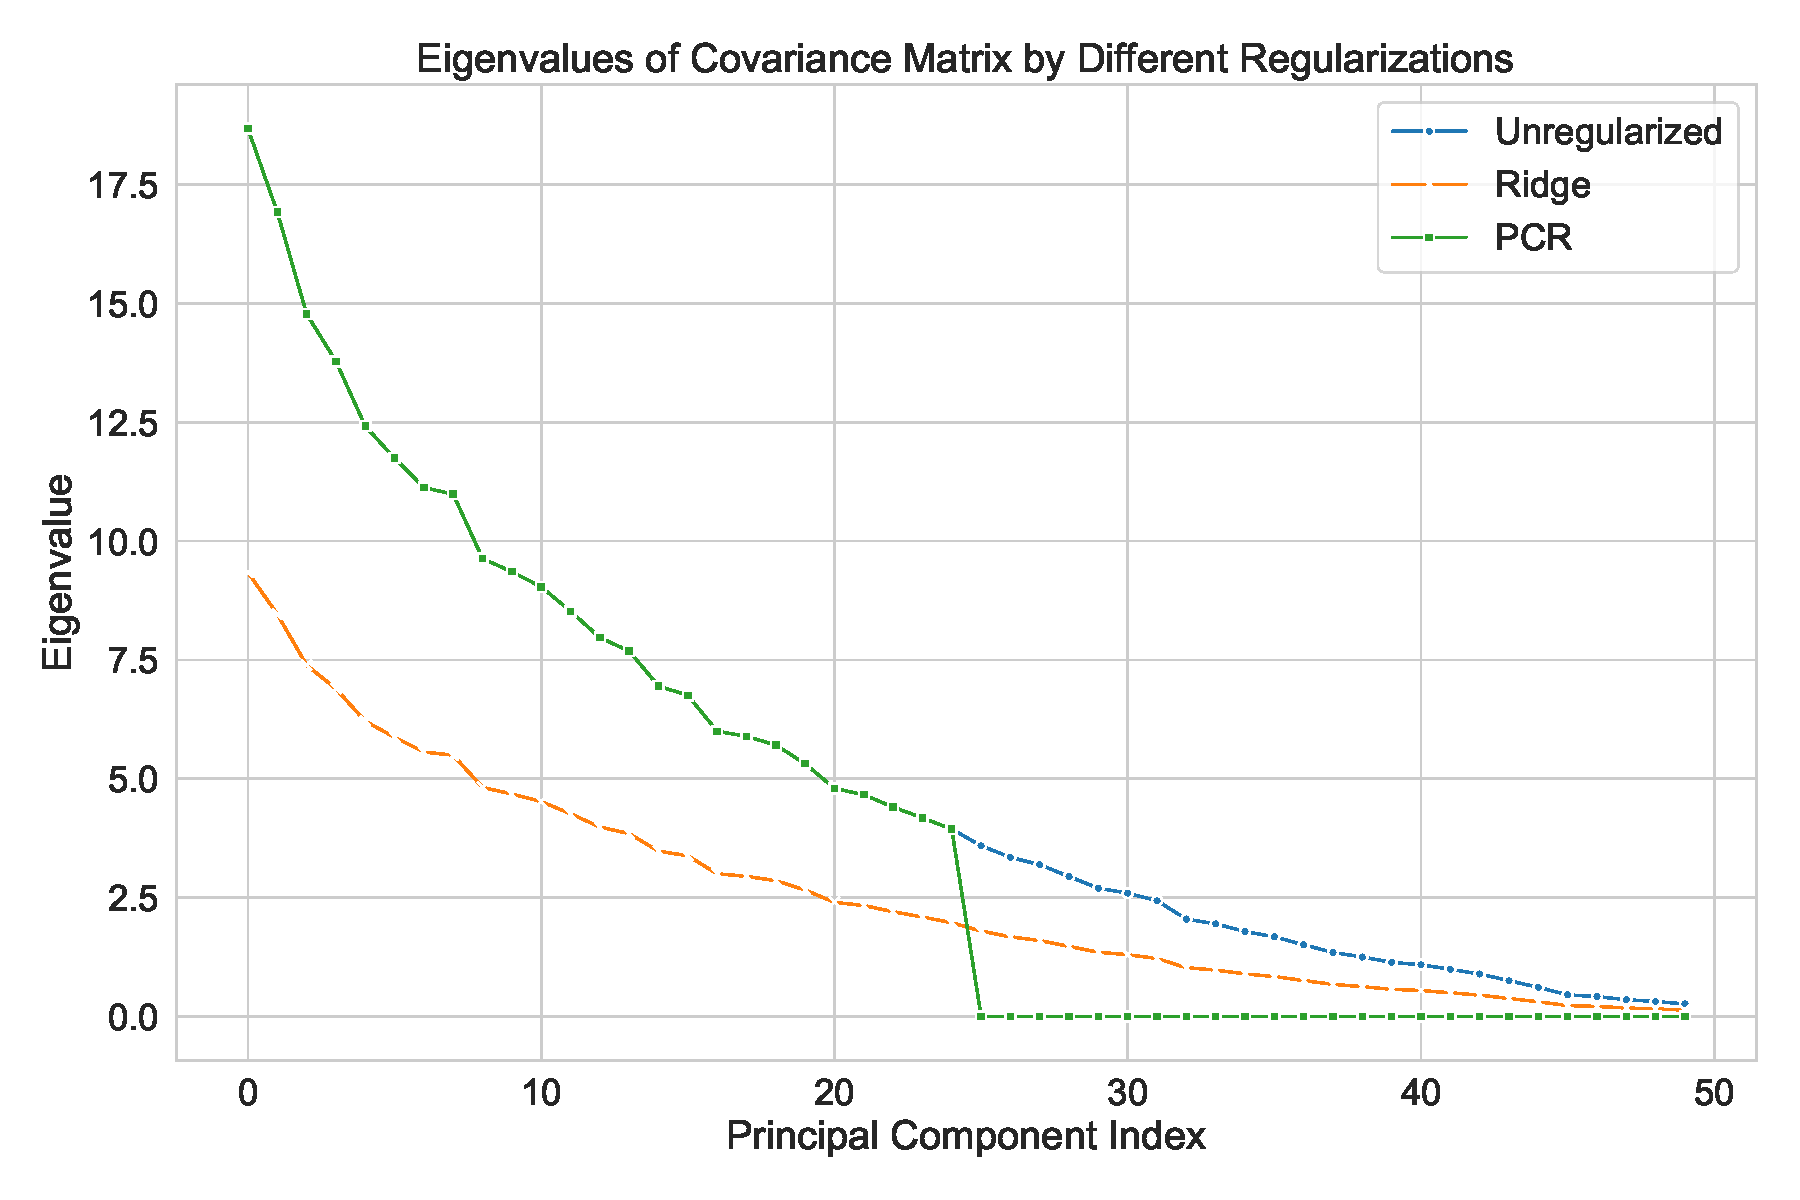
\includegraphics[width=0.8\textwidth]{figures/shrinkage/shrinkage}
    \caption{Comparison of the effect of OLS, Ridge, and PCA-CCA regularization on the eigenvalues of the covariance matrix.}\label{fig:shrinkage}
\end{figure}

The visualization underscores the intrinsic nature of each regularization method:
\begin{itemize}
    \item \textbf{Unregularized}: Presents the unaltered spectrum, making it susceptible to noise but preserving potential subtle patterns.
    \item \textbf{Ridge}: Applies consistent shrinkage across all components, reducing noise but possibly attenuating genuine signal.
    \item \textbf{PCA}: Focuses on dominant patterns by shrinking smaller components, potentially missing subtle connections but offering a cleaner representation of strong associations.
\end{itemize}
The choice between these shrinkage techniques should in general be based on the nature of the data.
We now transition to another essential regularization technique: sparse regularization.
While shrinkage aims to prevent overfitting by pulling weight estimates towards zero to reduce variance, sparse regularization aims to set weights to zero with the added benefit of enhancing model interpretability.

\subsubsection{Sparse Regularization}

Sparse regularization is a powerful tool for improving the performance and interpretability of linear models.
Sparse regularization encourages the model to use only a subset of the features, which can help to avoid overfitting and improve the interpretability of the model.
Sparse regularization works on the premise that only a subset of the features are relevant to the model.
Sparsity is typically achieved by adding either an L1 penalty or constraint\footnote{The L0 norm of the weight vector is the number of non-zero elements in the vector and is arguably a closer match to the goal, but the L0 norm is (a) not a proper norm in the mathematical sense and (b) not convex and so is difficult to optimize.}.
The L1 penalty is defined as:

\begin{align}
    \|u\|_1 = \sum_i |u_i|
\end{align}

Intuitively, this is the sum of the absolute values of the elements of the vector.
Now, with a foundational understanding of sparse regularization, we review a number of approaches to adding sparsity to the CCA problem.

\paragraph{Sparse PLS: Penalized Matrix Decomposition}
Penalized Matrix Decomposition (PMD)~\citep{witten2009penalized} provides an approximate solution to the sparse CCA problem by altering the constraints of the classical CCA formulation.
Specifically, PMD replaces the constraints \(u\spstop{i} \hat{\Sigma_{ii}} u\sps{i} = 1\) with \(u\spstop{i} u\sps{i}= 1\) and additionally imposes.
The optimization problem for PMD is then given by:

\begin{align}
    & u^{opt}=\underset{u}{\mathrm{argmax}}\{ u\spstop{1} \hat{\Sigma_{12}} u\sps{2} \} \\
    & \text{subject to:} \notag \\
    & u\spstop{1} u\sps{1} = 1 , u\spstop{2} u\sps{2} = 1 \notag \\
    & \|u\sps{1}\|_1 \leq \tau_1 , \|u\sps{2}\|_1 \leq \tau_2 \notag
\end{align}

Despite its influence, this method effectively performs Sparse PLS (SPLS) rather than Sparse CCA as in the original work.
For this reason, we refer to this method as SPLS in the rest of this thesis.
There are a number of other sparse CCA methods that employ a similar assumption to SPLS\citep{parkhomenko2009sparse, waaijenborg2008quantifying}.

While SPLS is an extremely efficient method (it can be solved by iteratively multiplying $u\sps{1}$ by $\hat{\Sigma_{12}}$ and soft thresholding), it is clear that it is not always a good approximation to the sparse CCA problem.

A number of approaches to Sparse CCA instead adopt a penalized least squares approach.

\paragraph{Sparse CCA: Least Squares Approaches}

It is well known that the CCA problem can be formulated as a constrained least squares problem with the intuition that
for \(X\sps{1} u\sps{1}=1\) and \(X\sps{2} u\sps{2}=1\), correlation is maximized when the squared distance
between \(X\sps{1} u\sps{1}\) and \(X\sps{2} u\sps{2}\) is minimized. \citep{golub1995canonical} proved the
convergence of a simple algorithm which alternates between solving the least squares problem for \(u\sps{1}\) and
\(u\sps{2}\) while keeping the other fixed.

With this intuition, \cite{wilms2015sparse} and \cite{mai2019iterative} separately proposed iterative penalized least
squares methods for sparse CCA\@.

\begin{align}
    \label{eq:mai}
    u^{opt} &= \underset{u}{\mathrm{argmin}} \left\{ \|X\sps{1}u\sps{1} - X\sps{2}u\sps{2}\|_2^2 + P(u) \right\} \\
    &\text{subject to:} \notag \\
    &u\spstop{1} \hat{\Sigma_{11}} u\sps{1}=1 \notag \\
    &u\spstop{2} \hat{\Sigma_{22}} u\sps{2}=1 \notag
\end{align}

Where \(P(u)\) is a penalty function.
The penalty term can be any function that penalizes the norm of the vector \(u\).
\citep{mai2019iterative} proved that solving the subproblems where one of $u\sps{i}$ is fixed is easy for one-homogenous $P$ where
\( P((\mu + 1)\theta) = (\mu + 1)P(\theta) \) which notably includes the lasso penalty.
This means a sparse CCA based
on alternating lasso regressions can be solved relatively efficiently using existing solvers.
However, the one homogenous penalty in practice limits the flexibility of the method.
For example, the elastic net penalty is not one-homogenous and therefore cannot be used with this method.\citep{
    kanatsoulis2018structured} proposed solving equation~\ref{eq:mai} for more general classes of $P$ using the
alternating direction method of multipliers (ADMM)~\citep{boyd2011distributed}.

The method most similar to ours is the sparse CCA by \cite{fu2017scalable}.
They use a classical CCA formulation, sometimes called the MAXVAR formulation, which views the problem as a constrained least squares with an auxiliary representation $T$\citep{carroll1968generalization,kettenring1971canonical}.


\begin{align}\label{eq:fu}
    \underset{U, T}{\mathrm{argmin}}\left\{\sum_i \|X\sps{i} U\sps{i} - T\|_F^2\right\}\\
    \text{subject to: }T^\top T = I\\
\end{align}

In this formulation, \(U\sps{i}\) represents the weights for the $i^{\text{th}}$ view, and \(T\) denotes the latent variable matrix.
The premise is that when \(T\) closely mirrors \(X\sps{i} U\sps{i}\) across all \(i\), the scores correlate.
Notably, this method is adaptable to multiple views.
The authors employed proximal gradient descent for regularization, specifically suited for penalties like the lasso.
Having discussed the benefits of both shrinkage (e.g., PCA-CCA, Ridge CCA, PLS) and sparsity (SPLS, Sparse CCA) in handling high-dimensional, noisy data, a natural progression is to integrate these advantages.
Specifically, the challenge lies in fusing shrinkage and sparsity within the CCA framework, enhancing the interpretability and performance of Brain-Behaviour association models.
The solution?
A method that employs readily available regularized regression solvers, allowing for flexible and tunable regularization in CCA.
This leads us to introduce the Flexible Regularized Alternating Least Squares (FRALS).

\section{Methods}

In this section, we outline the methodologies employed in our study for Canonical Correlation Analysis (CCA) and related techniques.
We first introduce the Flexible Regularized Alternating Least Squares (FRALS)—a versatile solution to the regularized CCA problem that incorporates various regularization functions, notably the elastic net penalty\cite{zou2005regularization}.
We then outline our experimental design, which assesses the performance of FRALS and other CCA variants, aiming to understand the effects of regularization on model performance and clarity.
Lastly, we specify the parameters and sources of the datasets used.

\subsection{Flexible Regularized Alternating Least Squares (FRALS)}\label{subsec:flexible-regularized-alternating-least
-squares-(frals)}

Consider the formulation in equation~\ref{eq:fu} for a single latent variable \(t\) with regularization $\lambda_i P_i$ on the weights \(u\sps{i}\).

\begin{align}
    \underset{u}{\mathrm{argmin}}\left\{\sum_i \|X\sps{i} u\sps{i} - t\|_2^2 + \textcolor{red}{\lambda_i P_i(u\sps{i})} \right\}\\
    \text{subject to: }t^\top t = 1\\
\end{align}

We can break this down into three subproblems.
The first subproblem for the auxiliary variable \(t\):

\begin{align}
    \underset{t}{\mathrm{argmin}}\left\{\sum_i \|X\sps{i} u\sps{i} - t\|_2^2\right\}\\
    \text{subject to: }t^\top t = 1\\
\end{align}

is a standard least squares problem, and can be solved in closed form by taking the average of $X\sps{i} u\sps{i}$ and normalizing.
Recall from section~\ref{subsec:generative-perspectives-on-cca} that this makes $t$ an estimate of the latent variables.

The second two subproblems are for the weights \(u\sps{i}\):

\begin{align}
    \underset{u\sps{i}}{\mathrm{argmin}}\left\{\sum_i \|X\sps{i} u\sps{i} - t\|_2^2 + \textcolor{red}{\lambda_i P_i(u\sps{i})} \right\}\\
\end{align}

Since the first subproblem is a regularized least squares problem, we can solve it using \textit{any regularized least squares solver}.
This gives our framework the flexibility for users to choose any regularization function with an appropriate solver including those optimised for neuroimaging data\citep{Nilearn_contributors_Nilearn} or specialised hardware including GPU acceleration\footnote{In principle, one could even plug in a neural network by replacing $X\sps{i} u\sps{i}$ with a neural network $f(X\sps{i})$.}.
In this work, we make use of the well-tested Elastic Net solver in the \texttt{scikit-learn} package~\citep{pedregosa2011scikit} where $P_i=\alpha_i \times \text{l1\_ratio} \|u\sps{i}\|_1 + \alpha_i \times (1-\text{l1\_ratio}) \|u\sps{i}\|^2_2$ so that we can tune the shrinkage and sparsity of the weights independently.

\subsection{The predictive framework for CCA}\label{subsec:the-predictive-framework-for-cca}

To evaluate the performance of CCA models, we employ a standard predictive framework.
We split the data into training and test sets using a 80:20 split, and use the training set to fit the model.
We then use the test set to evaluate the model's performance.
Where relevant, pre-processing is performed on the training set and the same pre-processing is applied to the test set.
This is important to avoid data leakage, where information from the test set is used to fit the model.

\subsubsection{Model Selection}

For the models that require hyperparameter tuning, we use a grid search to find the best hyperparameters.
Specifically, we use 5-fold cross-validation to evaluate the performance of a model with a given set of hyperparameters on 5 different splits of the training data with non-overlapping validation sets.
We optimise for the hyperparameters that give the best average out of sample correlation.

\subsubsection{Model Comparisons}
We employ several CCA variants for this experiment, including Canonical Correlation Analysis (CCA), Partial Least Squares (PLS), and more.

\begin{table}[h]
\centering
\caption{Employed CCA Variants}
\begin{tabular}{|l|l|l|l|}
\hline
\textbf{Model} & \textbf{Abbreviation} & \textbf{Hyperparameters}  \\
\hline
Canonical Correlation Analysis & CCA & -   \\
\hline
Regularized CCA & RCCA & \(c_1, c_2\)   \\
\hline
Partial Least Squares & PLS & -   \\
\hline
Sparse PLS & SPLS & \(\tau_1, \tau_2\)   \\
\hline
FRALS - Elastic & Elastic & \(\alpha_1, \alpha_2, \text{l1}_1, \text{l1}_2\)   \\
\hline
Principal Component Analysis & PCA & -  \\
\hline
\end{tabular}\label{table:cca-variants}
\end{table}

\subsection{Datasets}\label{subsec:datasets}

The datasets employed in our experiments comprise the HCP and ADNI data.
These datasets provide insights into brain functionality and behavior from different perspectives.
We chose the HCP and the ADNI datasets based on 2 recent landmark studies and the tutorial paper this chapter is loosely related to \cite{mihalik2022canonical}.

\paragraph{The Human Connectome Project (HCP)} offers publicly available resting-state functional MRI (rs-fMRI) and non-imaging measures like demographics, psychometrics, and other behavioral measures.
Specifically, we sourced data from 1003 subjects out of the 1200-subject data release of the HCP.
This dataset is constructed using brain connectivity features of the thoroughly processed rs-fMRI data.
This processing results in 19,900 brain variables for every subject.
Additionally, there are 145 non-imaging measures employed.
Notably, nine confounding variables were regressed out from both data modalities.
Each variable was standardized for zero mean and unit variance.
More details can be found in \cite{smith2015positive, mihalik2022canonical}.
We summarize the parameters of the HCP data in table~\ref{tab:hcp-parameters}.

\begin{table}
\centering
\caption{HCP Data Parameters}
\begin{tabular}{| l | l |}
\hline
\textbf{Parameter} & \textbf{Value} \\
\hline
Number of samples (\textit{n}) & 1003 \\
Number of features in View 1 (\textit{p}) & 19900 \\
Number of features in View 2 (\textit{q}) & 145 \\
\hline
\end{tabular}\label{tab:hcp-parameters}
\end{table}

\paragraph{The ADNI} database is found at \url{adni.loni.usc.edu}.
Launched in 2003, ADNI's main objective is to assess the combination of serial MRI, PET (Positron emission tomography), biological markers, and clinical and neuropsychological assessment in tracking the progression of Mild Cognitive Impairment (MCI) and early Alzheimer’s disease.
For our experiments, we used a subset of 592 unique subjects from the ADNI. The MRI scans underwent a series of processing stages, yielding a grey matter probability map.
The Mini-Mental State Examination (MMSE) scores were employed to investigate the association with the grey matter maps.
Composed of a series of brief tasks, the MMSE evaluates various cognitive domains including memory, attention, language, and visuospatial skills.
The MMSE is a widely used test for assessing cognitive impairment.
The MMSE scores range from 0 to 30, with lower scores indicating more severe cognitive impairment.
We summarize the parameters of the ADNI data in table~\ref{tab:adni-parameters}.

\begin{table}
\centering
\caption{ADNI Data Parameters}
\begin{tabular}{| l | l |}
\hline
\textbf{Parameter} & \textbf{Value} \\
\hline
Number of samples (\textit{n}) & 592 \\
Number of features in View 1 (\textit{p}) & 168130 \\
Number of features in View 2 (\textit{q}) & 31 \\
\hline
\end{tabular}\label{tab:adni-parameters}
\end{table}

\section{Results}

\subsection{Human Connectome Project (HCP) Data}

Next, we consider the results of applying the various CCA variants to the HCP data.
Since the HCP data is high-dimensional, we drop CCA from the analysis since it would produce random results.

\subsubsection{Out of Sample Correlation}

The Elastic Net did not improve upon Ridge CCA in terms of holdout correlation captured (Figure~\ref{fig:performance}).
However, both Ridge CCA and ElasticNet outperformed PLS and SPLS.
This suggests that tunable L2 regularization is important, even for very high-dimensional data.
SPLS does however outperform PLS.

\begin{figure}
\centering
\includegraphics[width=0.5\linewidth]{figures/hcp/holdout_correlations}
\caption{Out-of-sample canonical correlations for each model.}
\end{figure}

\subsubsection{Behaviour Weights and Loadings}

Figure\ref{fig:behaviour} plots the top 8 positive and negative non-imaging loadings and their associated weights for each model\footnote{This can and does mean for example that a zero weight may have a non-zero loading!}.
This is to illustrate some of the effects we have observed in the previous section.
PCA finds a mode of variation in the behavioural data that is positively correlated with psychiatric and life function tests and negatively correlated with a number of emotion and personality tests.
The RCCA and ElasticNet models find a mode of variation in the behavioural data that is negatively correlated with the Line Orientation test and to a lesser extent smoking and positively correlated with a number of other cognitive tests.
The PLS model finds a mode of variation in the behavioural data that is somewhat similar to the `good-bad' mode in\cite{smith2015positive} with a positive correlation with agreeableness, vocabulary tests, and feelings about ones' life and a strong negative correlation with smoking, rule-breaking, and antisocial personality traits.
The SPLS mode is similar but selects out the rule-breaking and antisocial personality traits in favour of the vocabulary tests and smoking.

\begin{figure}
\centering
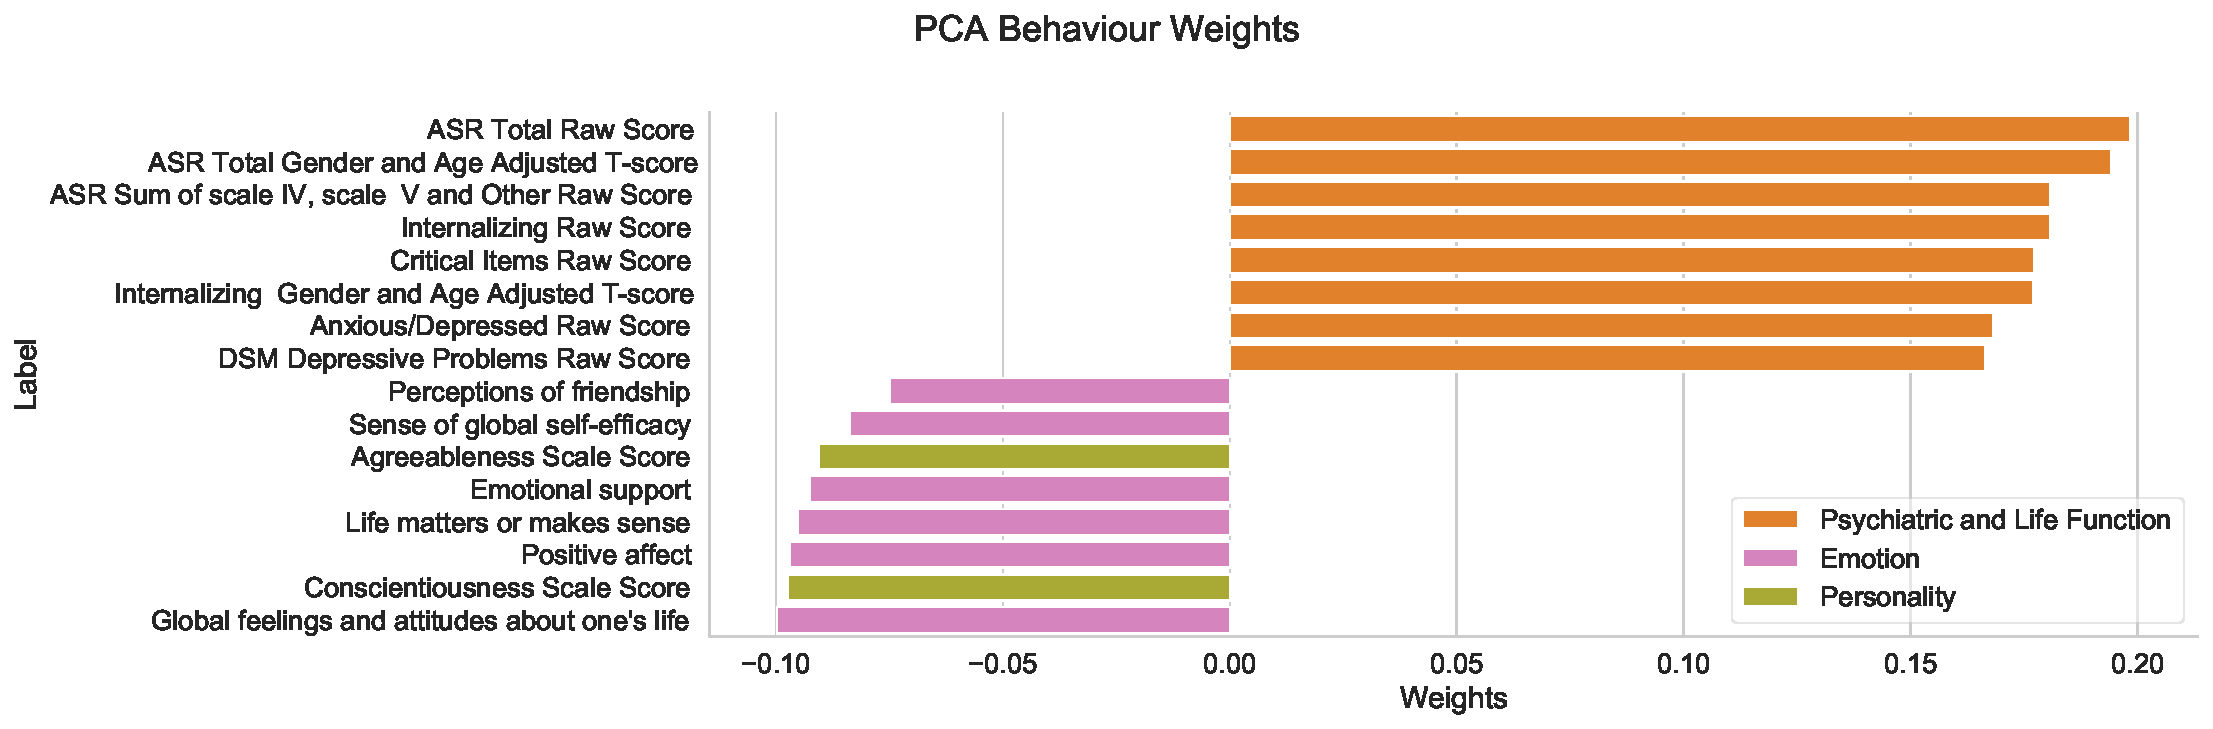
\includegraphics[width=0.8\linewidth]{figures/hcp/PCA behaviour weights}
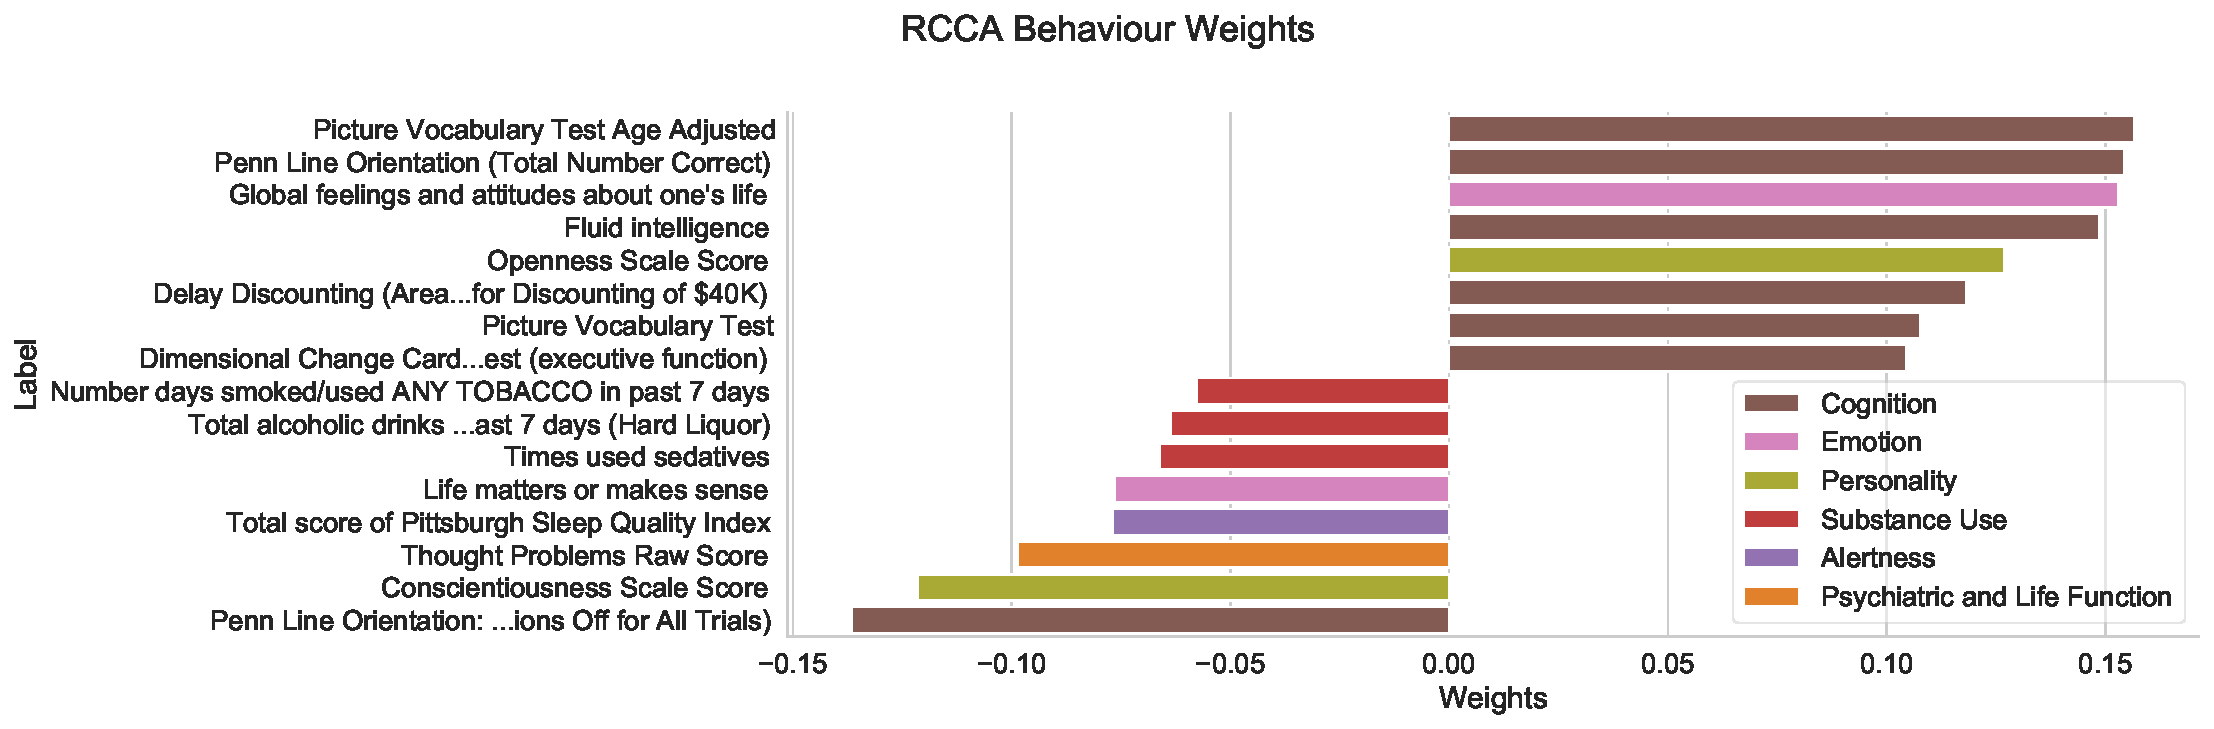
\includegraphics[width=0.8\linewidth]{figures/hcp/RCCA behaviour weights}
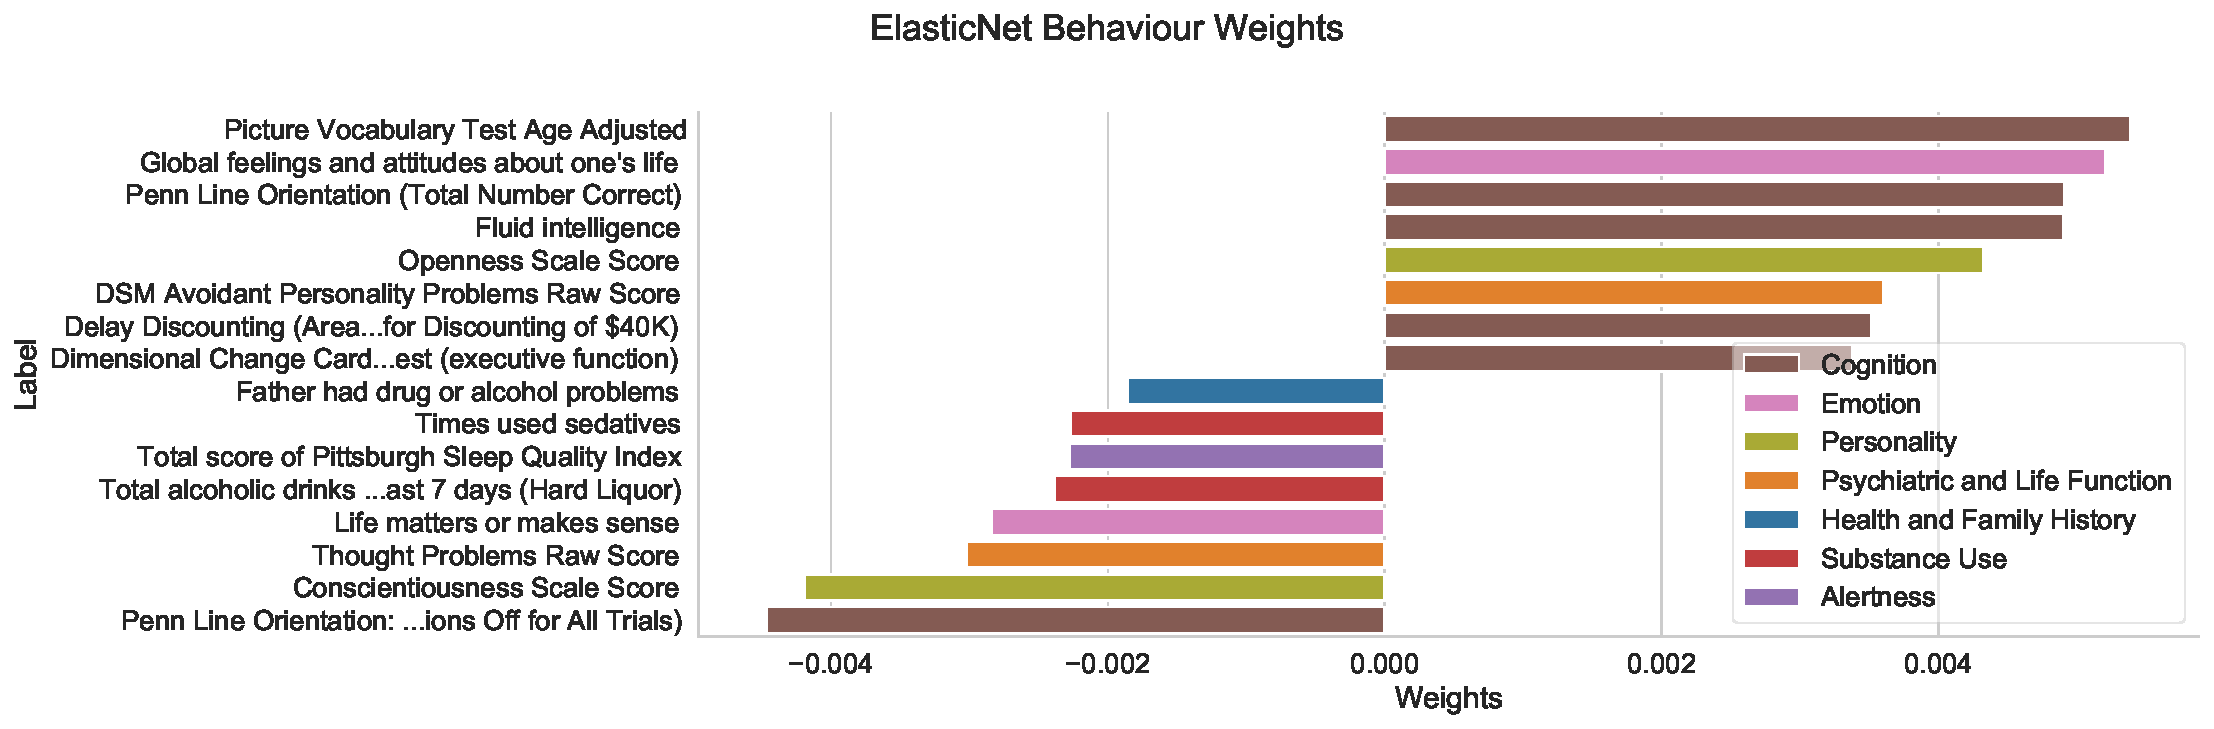
\includegraphics[width=0.8\linewidth]{figures/hcp/ElasticNet behaviour weights}
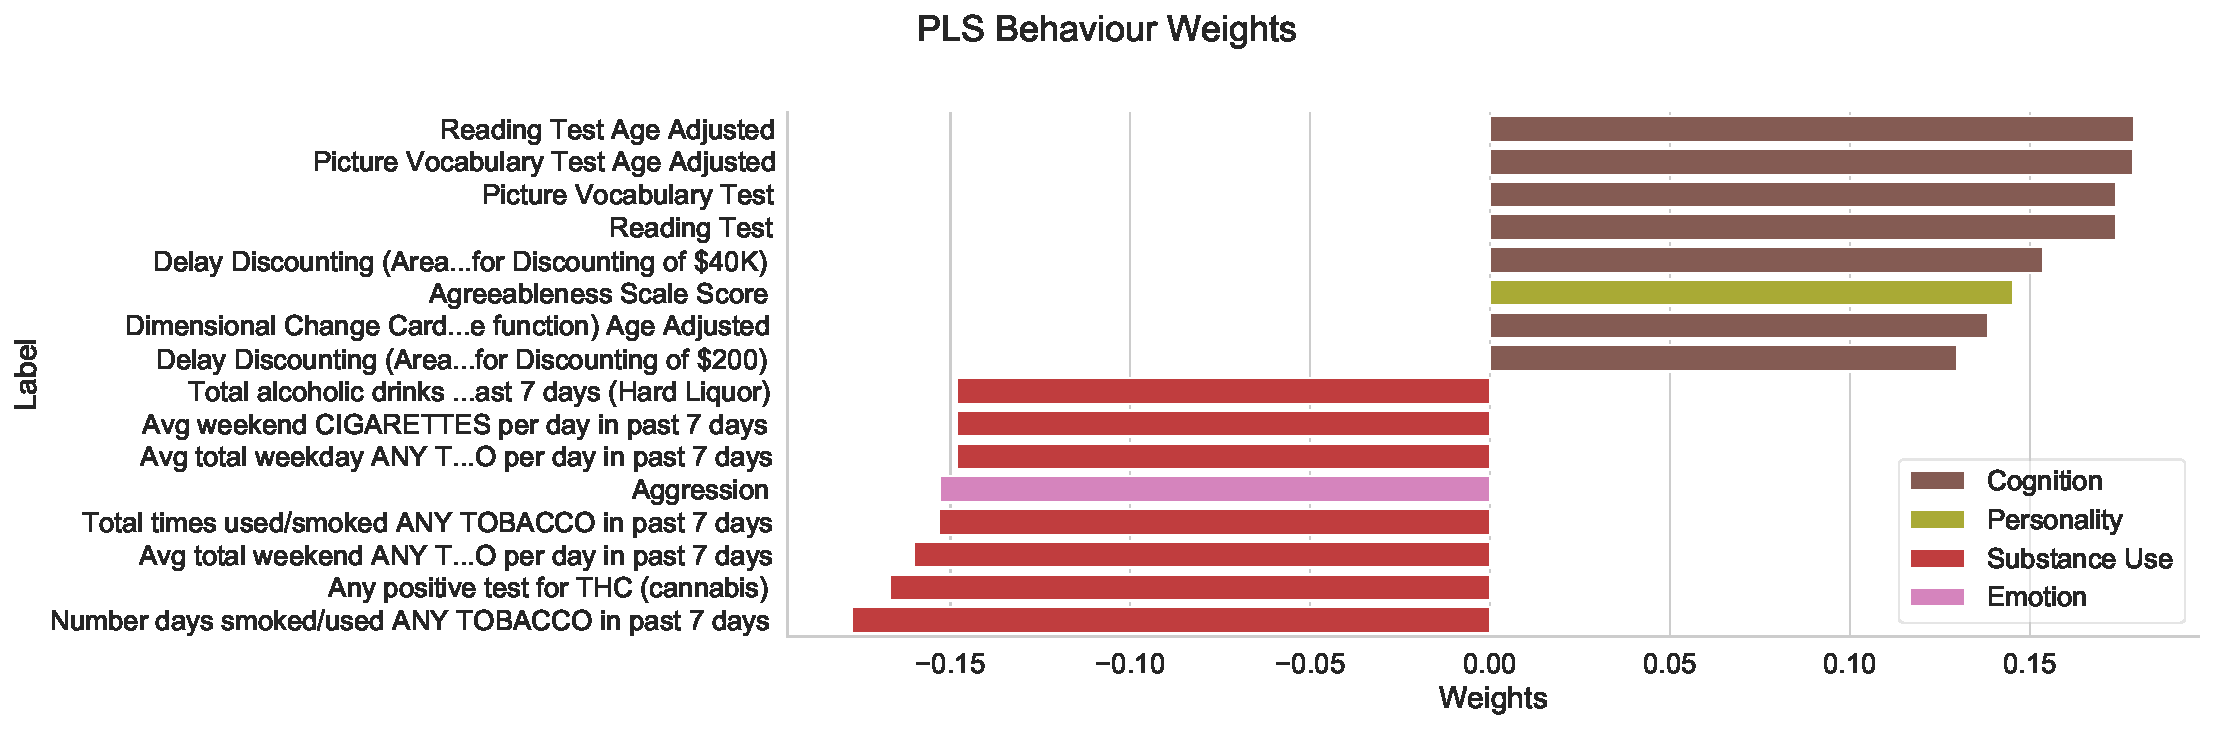
\includegraphics[width=0.8\linewidth]{figures/hcp/PLS behaviour weights}
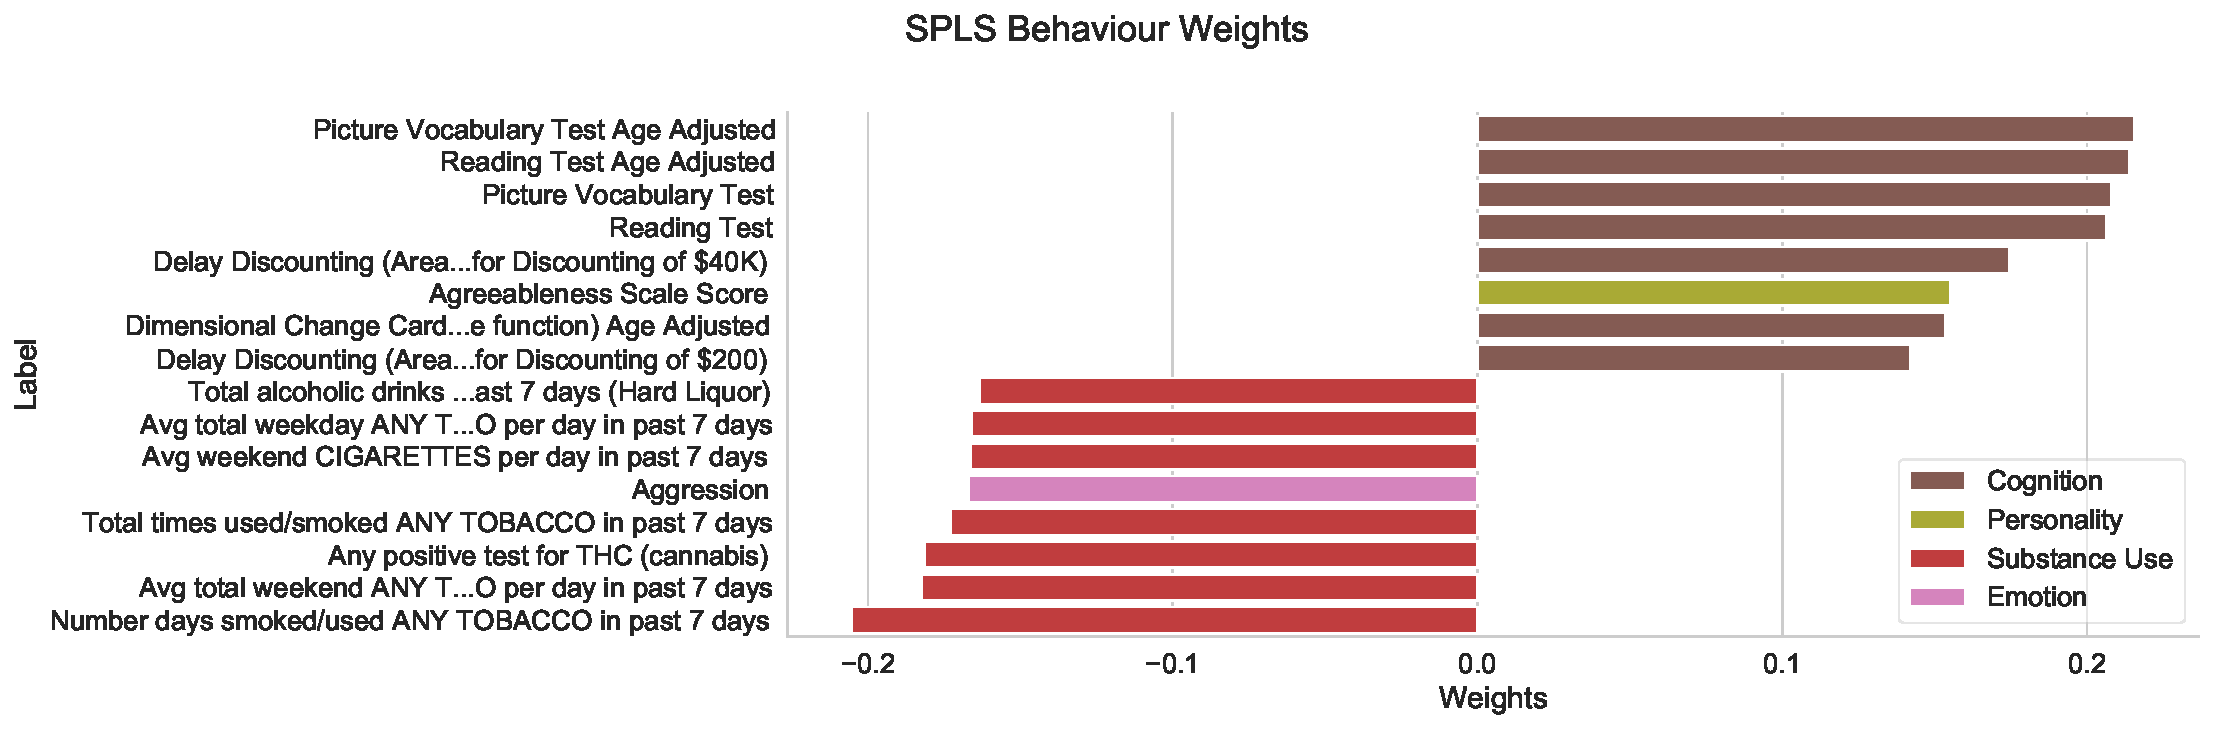
\includegraphics[width=0.8\linewidth]{figures/hcp/SPLS behaviour weights}
\caption{Top 8 positive and negative non-imaging loadings for each model}\label{fig:behaviour}
\end{figure}

\subsubsection{Brain Connectivity Weights and Loadings}

In this section, we use two different methods to visualize the brain connectivity weights and loadings.
The first method is to use chord diagrams to visualize the top 8 positive and negative brain weights and loadings for each model.
This approach is inspired by the chord diagrams used in \cite{smith2015positive}.
The second method is to use surface maps to visualize the brain connectivity weights and loadings.
This approach has been used by both \cite{ferreira2022hierarchical} and \cite{smith2015positive}.

\paragraph{Chord Diagrams}
We grouped the nodes of the connectivity matrix of our data into 7 parcels according to the Yeo 7 network parcellation\cite{yeo2011organization}.
These are then arranged around the circumference of the chord diagram using the Nichord package\cite{bogdan2023connsearch}.
The plots then show the 8 strongest positive and negative weights or loadings for each model as `chords'.
The chord diagrams in Figure~\ref{fig:chord_weights} and Figure~\ref{fig:chord_loadings} show the top 8 positive and negative brain weights and loadings for each model.

\textcolor{red} Need to find something biologically useful to say about these.

\begin{figure}
\centering
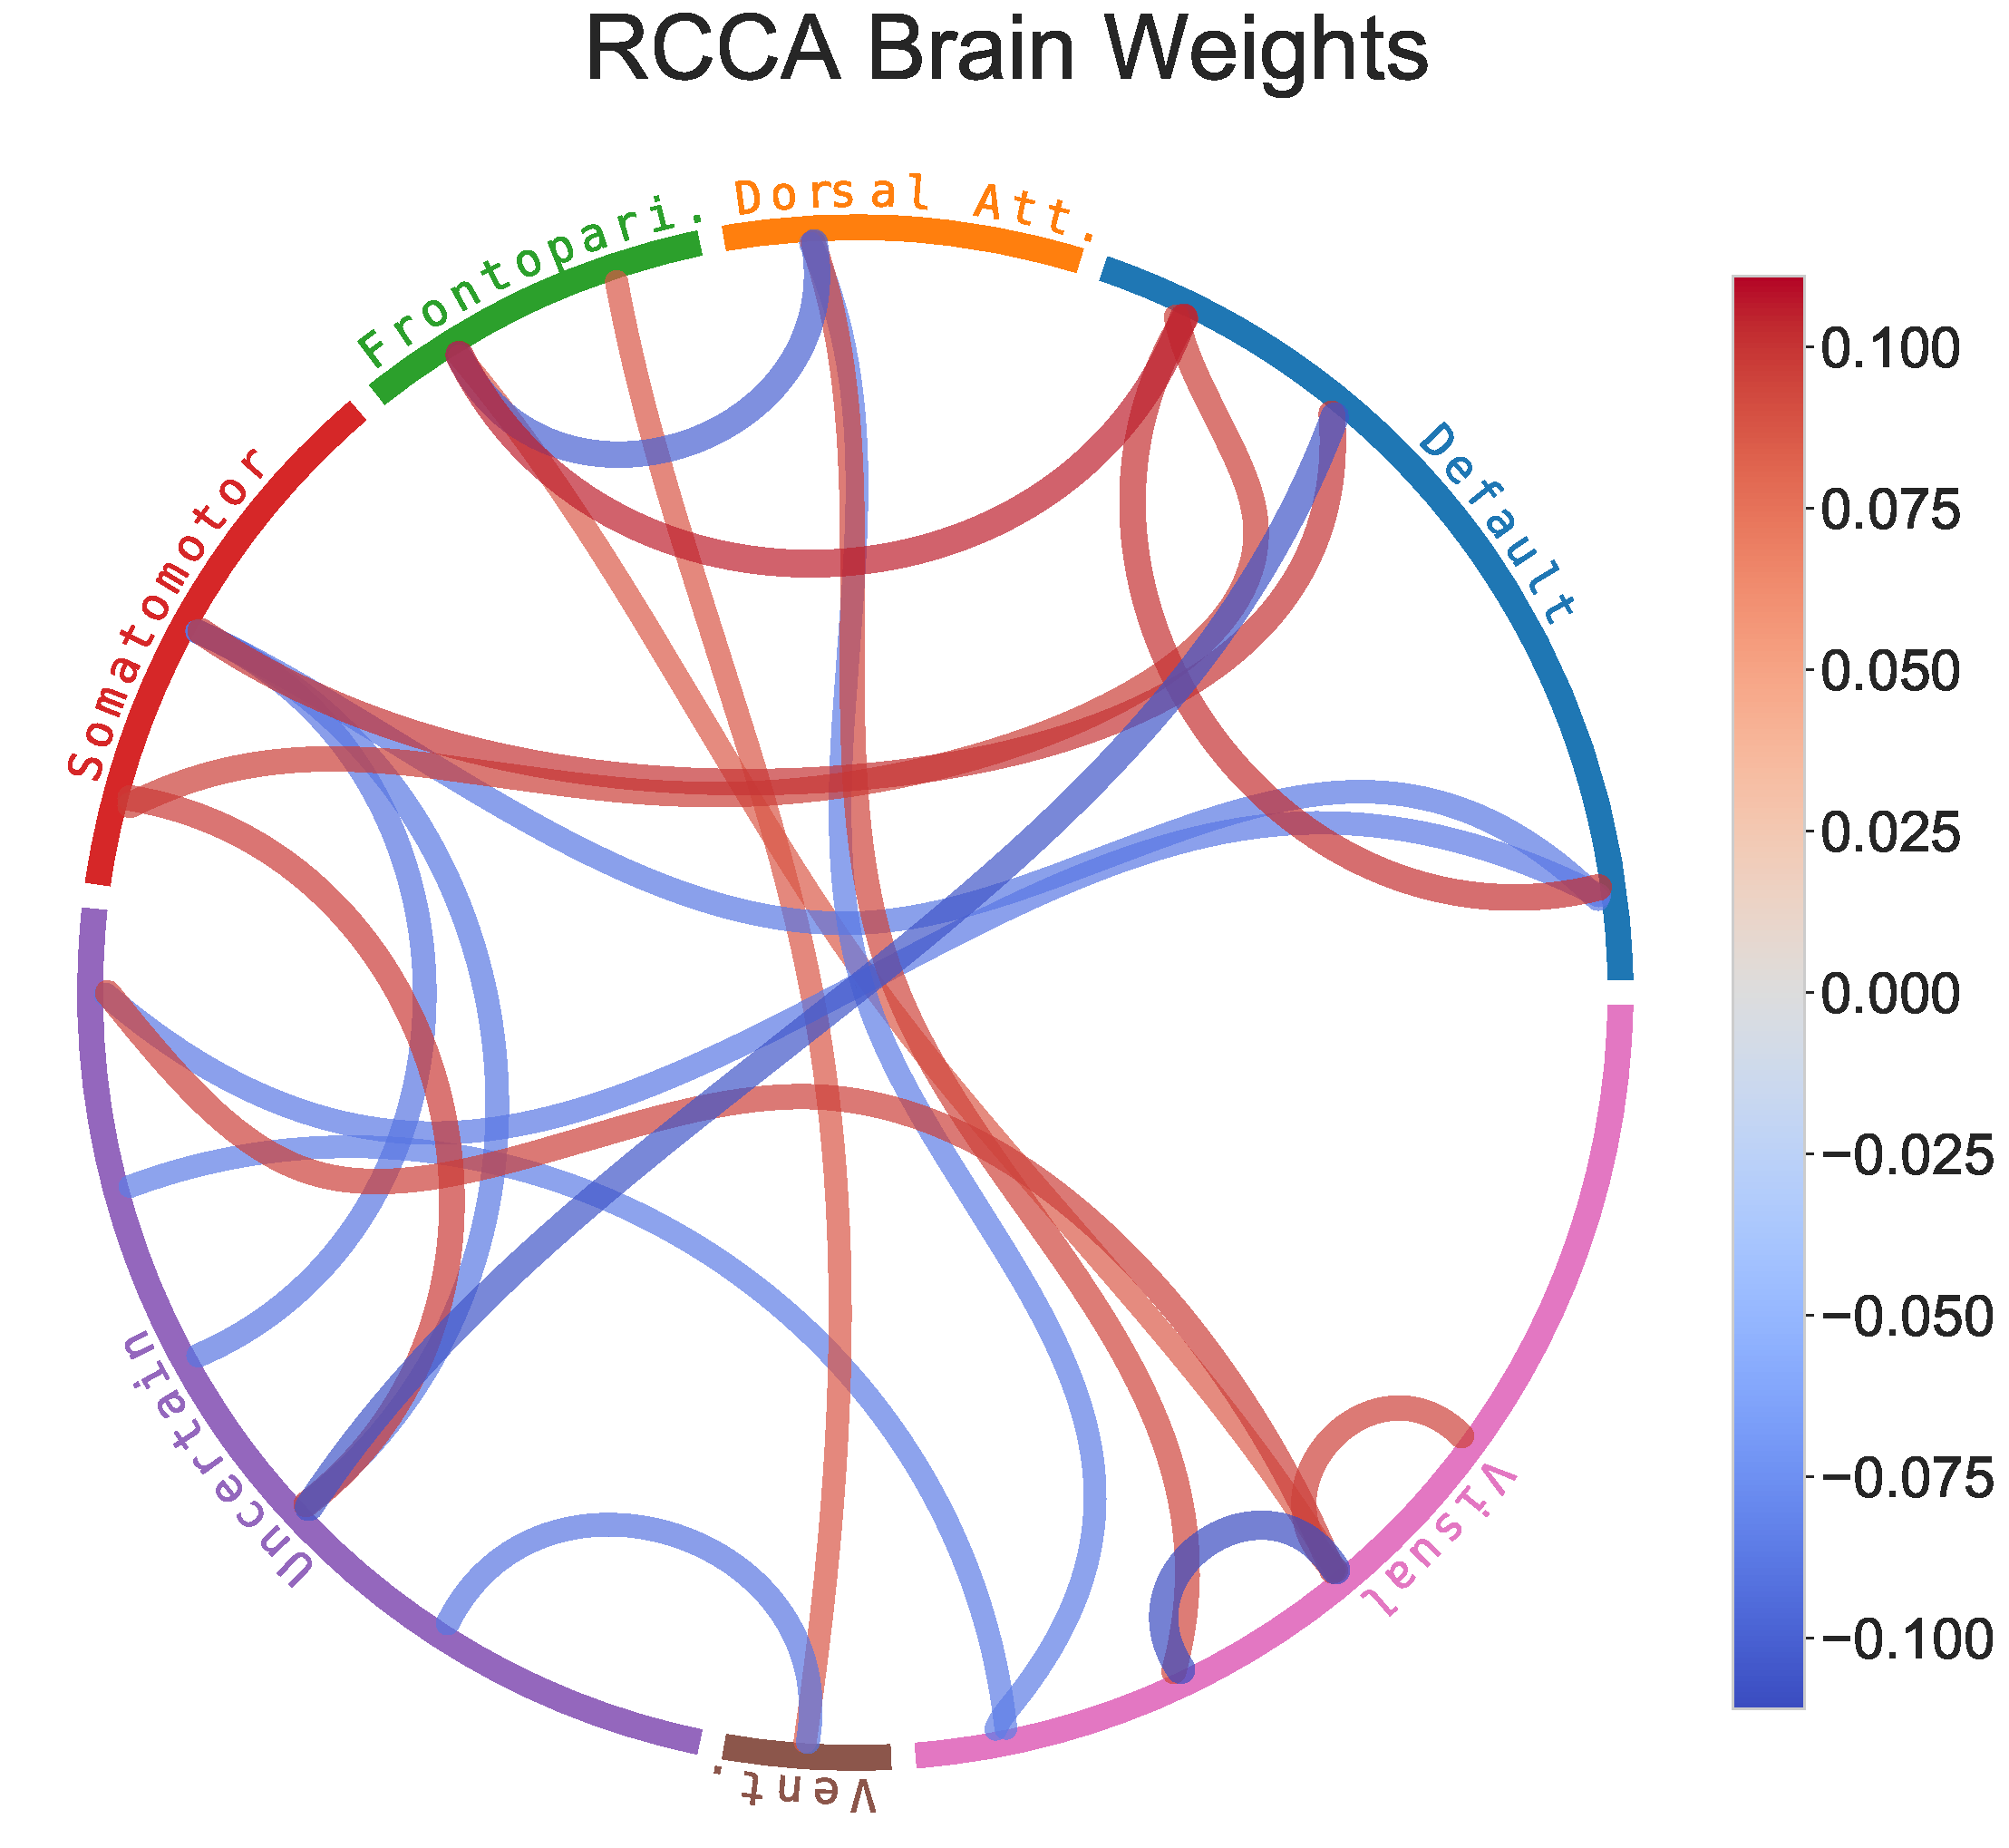
\includegraphics[width=0.49\linewidth]{figures/hcp/RCCA brain weights}
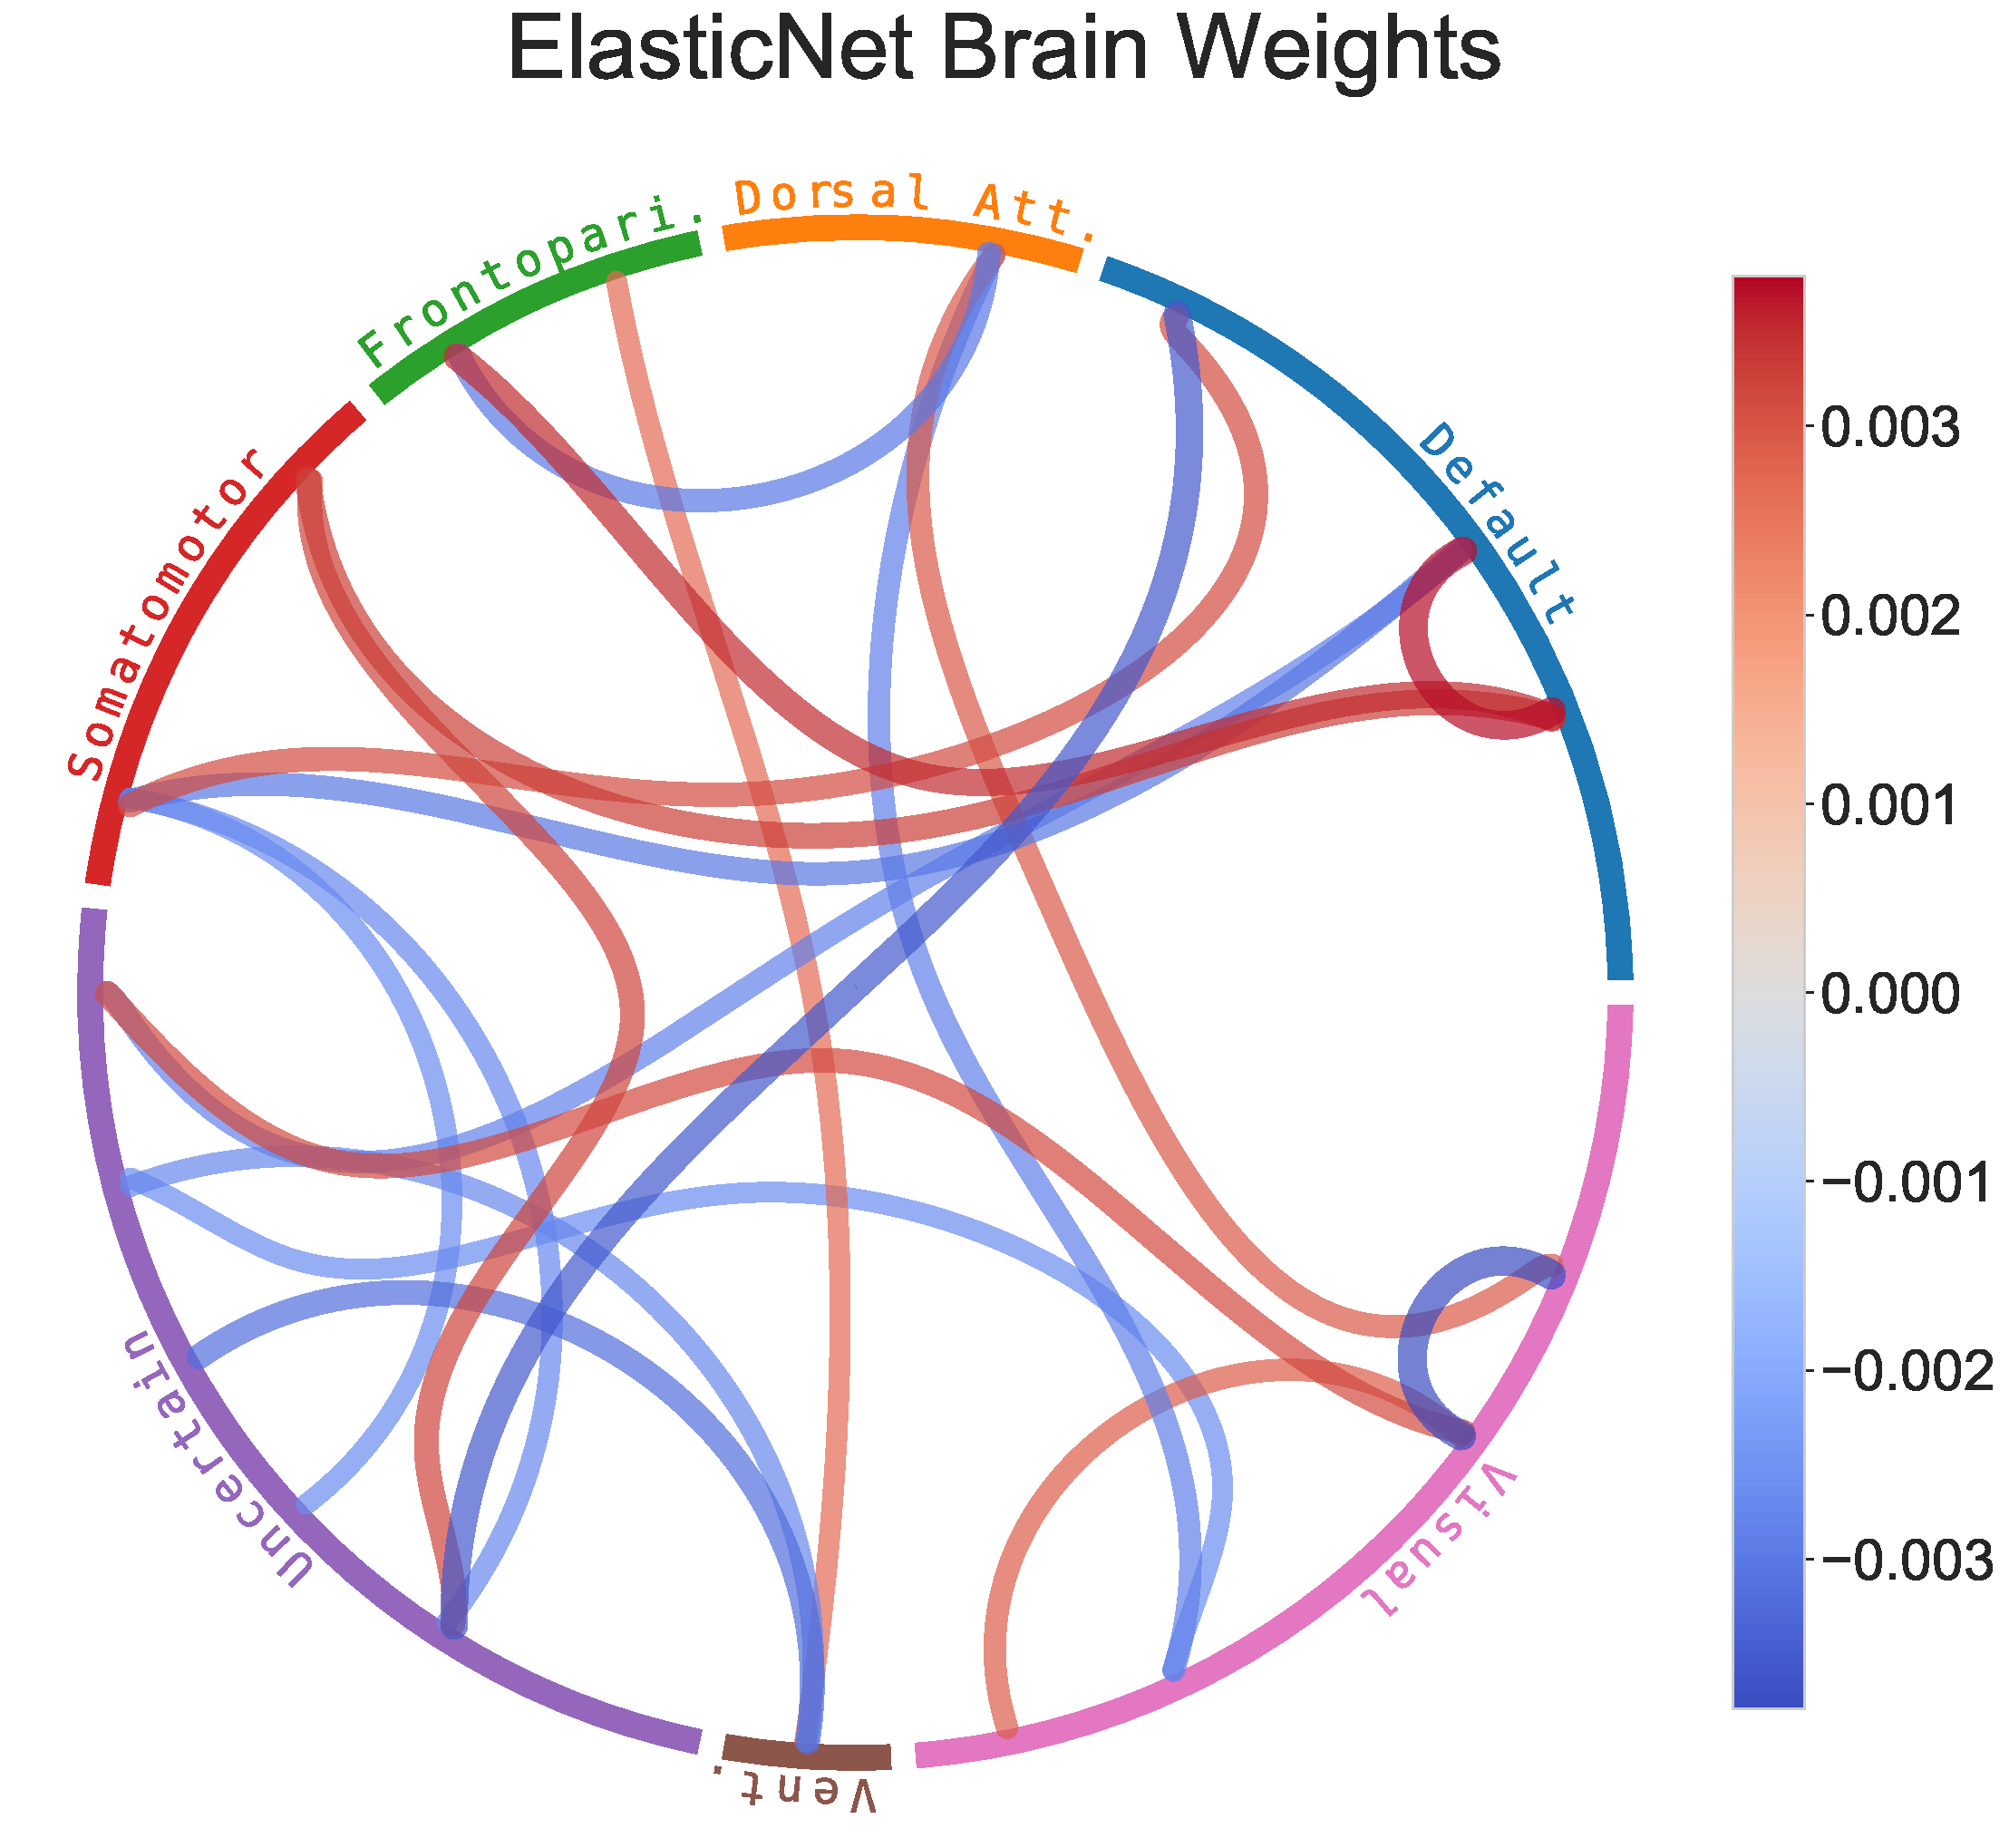
\includegraphics[width=0.49\linewidth]{figures/hcp/ElasticNet brain weights}
\includegraphics[width=0.49\linewidth]{figures/hcp/PLS brain weights}
\includegraphics[width=0.49\linewidth]{figures/hcp/SPLS brain weights}
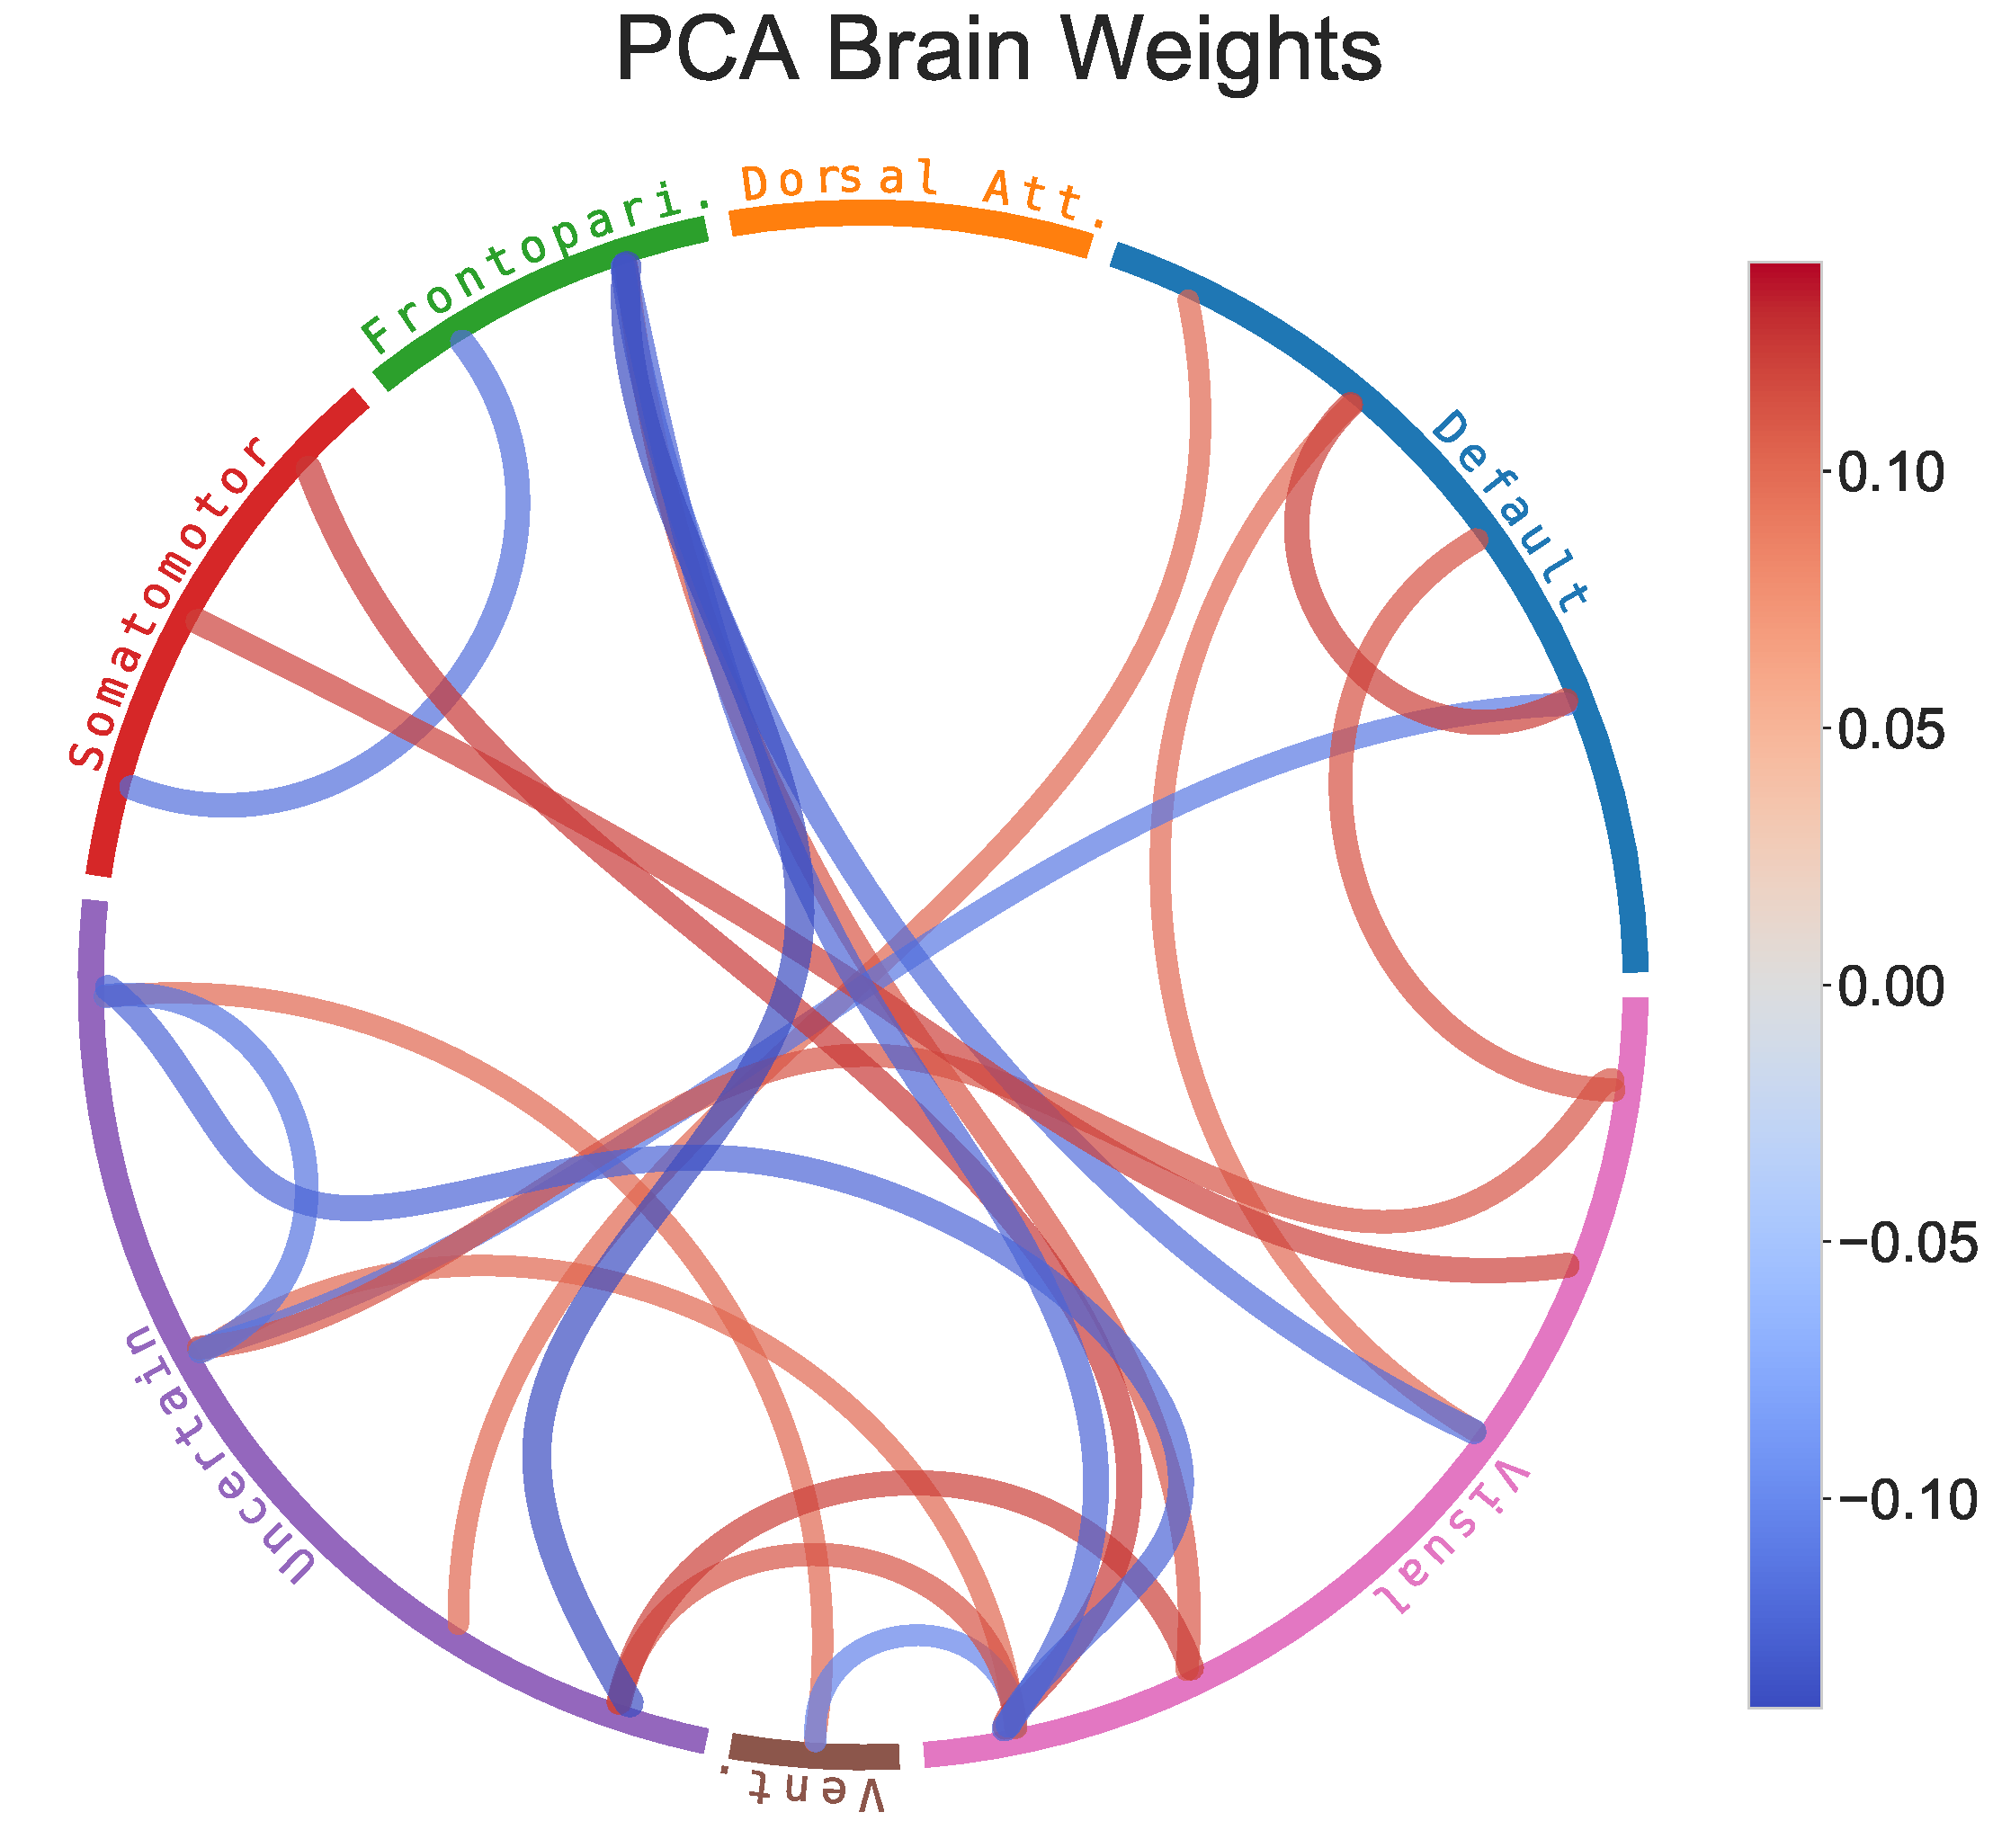
\includegraphics[width=0.49\linewidth]{figures/hcp/PCA brain weights}
\caption{Chord diagrams of the top 8 positive and negative brain weights for each model.}\label{fig:chord_weights}
\end{figure}

\paragraph{Surface Map Parcellations}
The brain surface plots in Figure~\ref{fig:brain} represent maps of brain connection strength increases/decreases, which
were obtained by weighting each node’s parcel map with the GFA edge-strengths summed across the edges
connected to the node.
In Figure~\ref{fig:brain}, we show increases on the left and decreases on the right.

\textcolor{red} Need to find something biologically useful to say about these.
%
%\begin{figure}
%\centering
%\includegraphics[width=\linewidth]{figures/hcp/PCA brain loadings surface}
%\includegraphics[width=\linewidth]{figures/hcp/RCCA brain loadings surface}
%\includegraphics[width=\linewidth]{figures/hcp/ElasticNet brain loadings surface}
%\includegraphics[width=\linewidth]{figures/hcp/PLS brain loadings surface}
%\includegraphics[width=\linewidth]{figures/hcp/SPLS brain loadings surface}
%\caption{Map of CCA connection strength variations, with each node’s parcel map weighted by CCA edge-strength changes across edges involving that node.}\label{fig:brain}
%\end{figure}

\subsubsection{Sparsity of Weights}

Table \ref{tab:brain-behaviour-weights-hcp} shows the number of non-zero weights for each model.
We can see that tuned SPLS and Elastic Net do find sparse weights, but given the minimal difference in performance, it is not convincing evidence that this is a useful property.

\begin{table}[h]
\centering
\caption{Number of non-zero weights for each model.}
\begin{tabular}{|c|c|c|}
\hline
Model &  Brain Weights &  Behaviour Weights \\
\hline
PCA & 300 & 145 \\
RCCA & 300 & 145 \\
Elastic Net & 241 & 96 \\
PLS & 300 & 145 \\
SPLS & 118 & 56 \\
\hline
\end{tabular}\label{tab:brain-behaviour-weights-hcp}
\end{table}

\newpage
\subsection{Alzheimers Disease Neuroimaging Initiative (ADNI) Data}\label{subsec:adni}

We now turn to the ADNI data where our analysis is similar but visualized differently.
This is because the ADNI data contains structural MRI data rather than functional MRI data.

\subsubsection{Out of Sample Correlation}

In this experiment, the Elastic Net model outperformed all other models in terms of out-of-sample correlation (Figure~\ref{fig:performance}).
The RCCA model also outperformed the PLS and SPLS models while SPLS outperformed PLS.
Suprisingly, PCA performed almost as well as PLS.

\begin{figure}
\centering
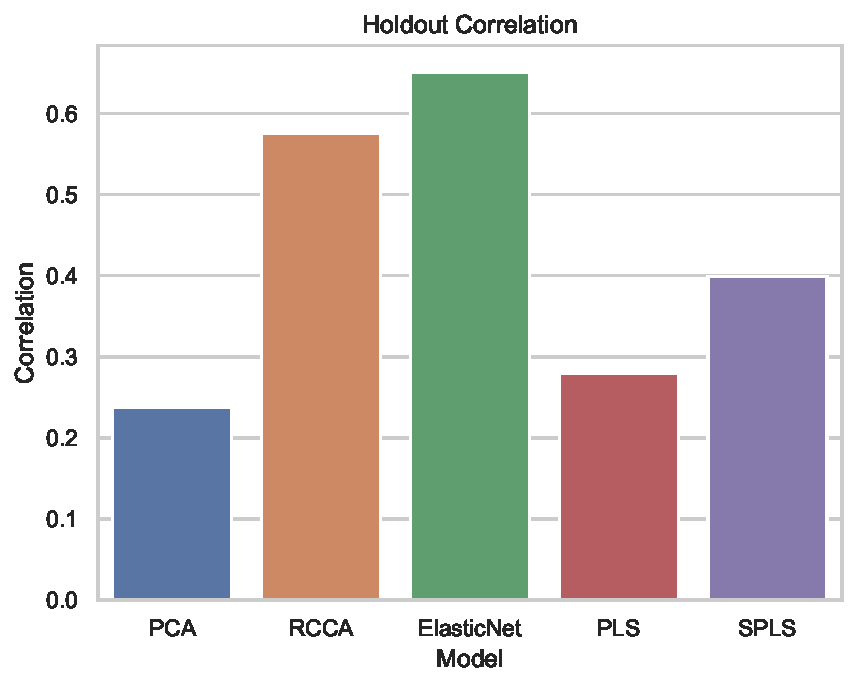
\includegraphics[width=0.5\linewidth]{figures/adni/holdout_correlations}
\caption{Out-of-sample canonical correlations for each model.}\label{fig:performance}
\end{figure}

\subsubsection{Behaviour Weights and Loadings}

As for the HCP data, Figure \ref{fig:adni-beh} plots the top 8 positive and negative non-imaging loadings and their associated weights for each model.
Some of the identified behavioural loadings including a number of orientation tests are similar across all of the models, including even PCA.
This is indicative of the strong shared signal between the behavioural data and the brain structure data.
SPLS and Elastic Net both hone in on the orientation and recall tests in the weight space, which appears also to translate to the loading space.
The RCCA and Elastic Net models are suprisingly different in both the weight and loading space, with the RCCA loading on a couple of attention and calculation tests in addition to the ubiquitous orientation and recall tests.

\begin{figure}
\centering
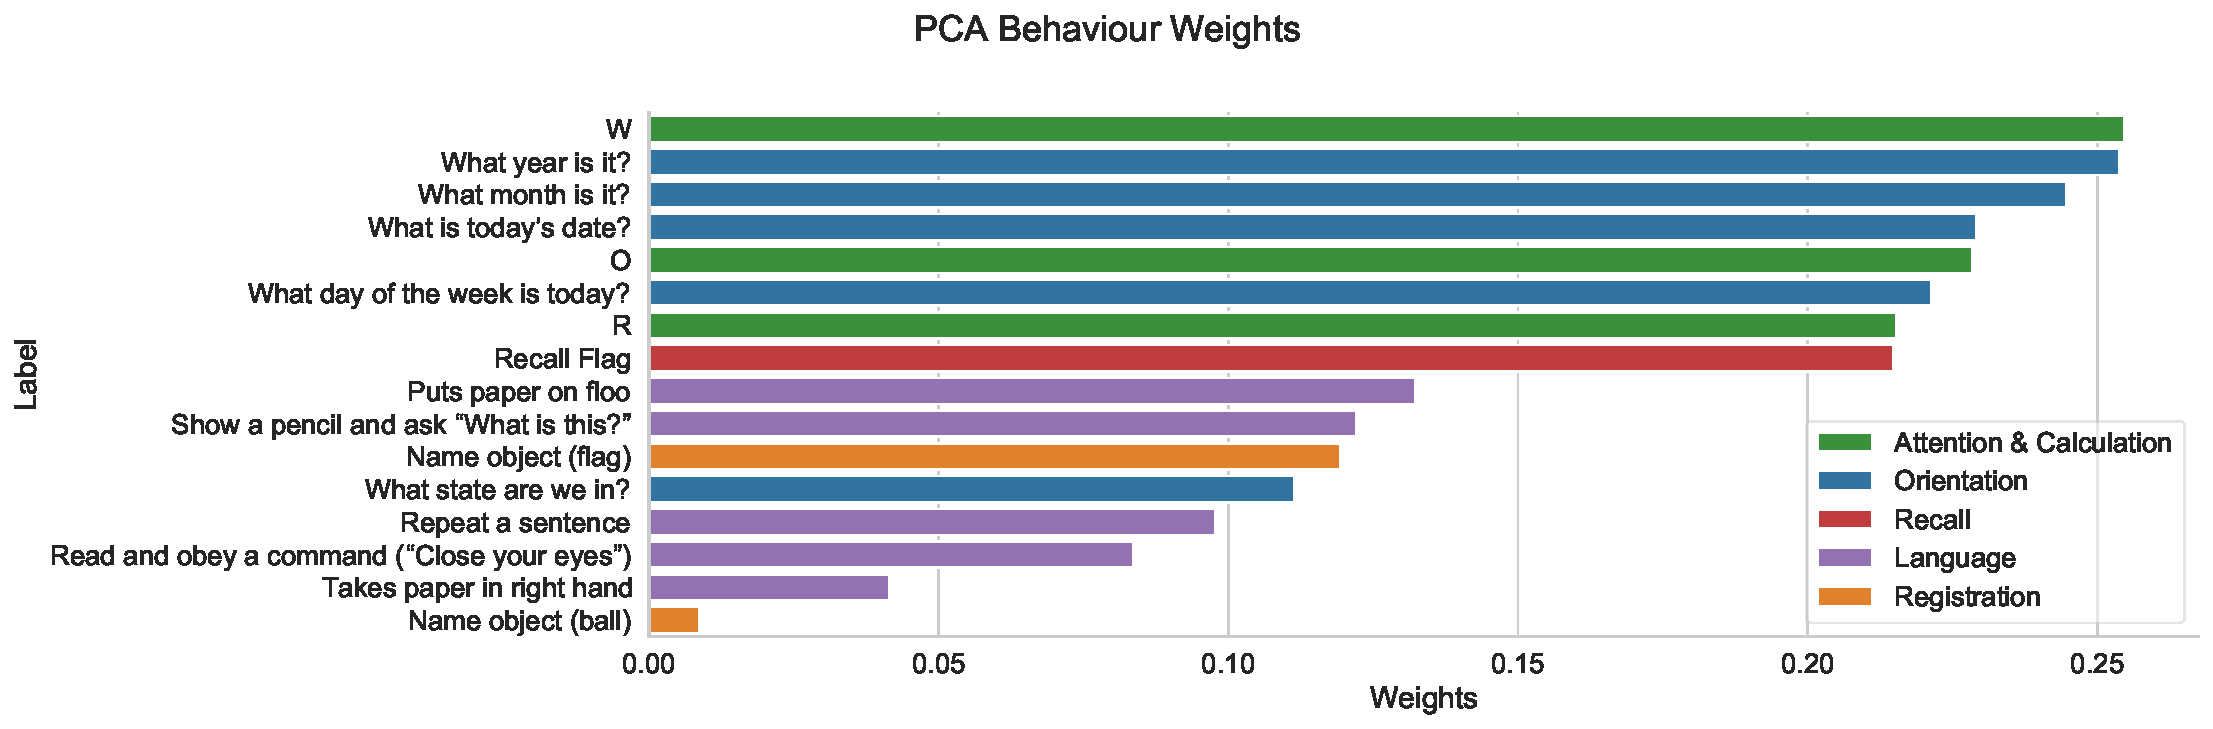
\includegraphics[width=0.8\linewidth]{figures/adni/PCA behaviour weights}
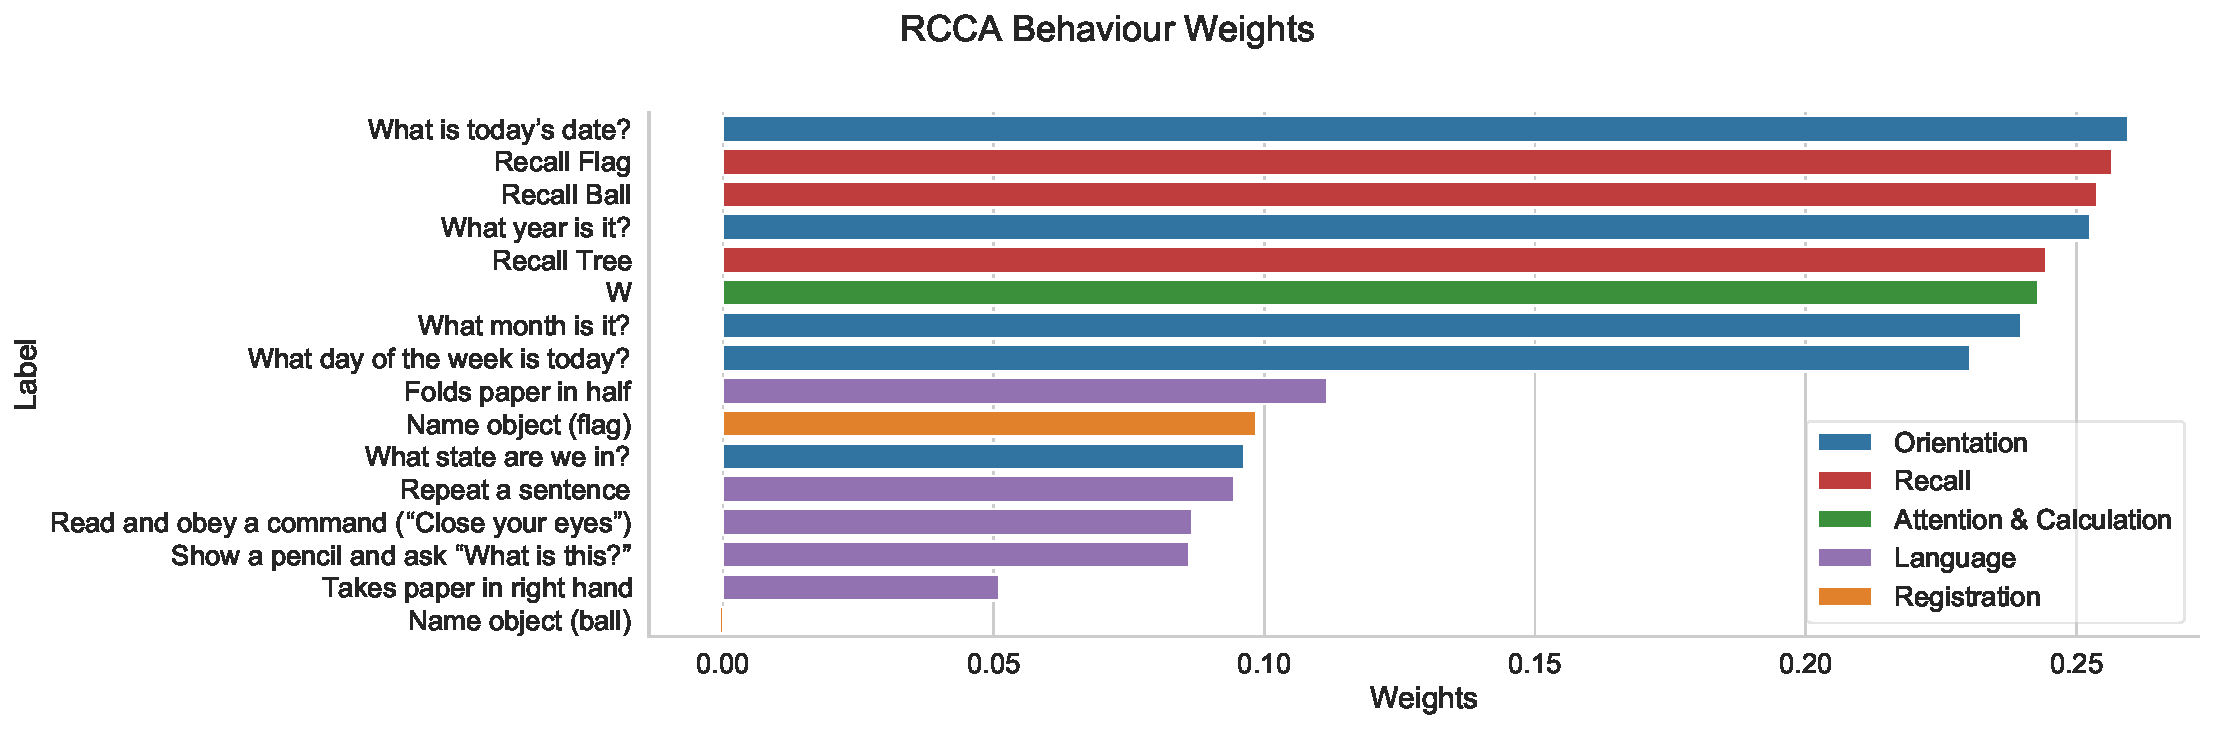
\includegraphics[width=0.8\linewidth]{figures/adni/RCCA behaviour weights}
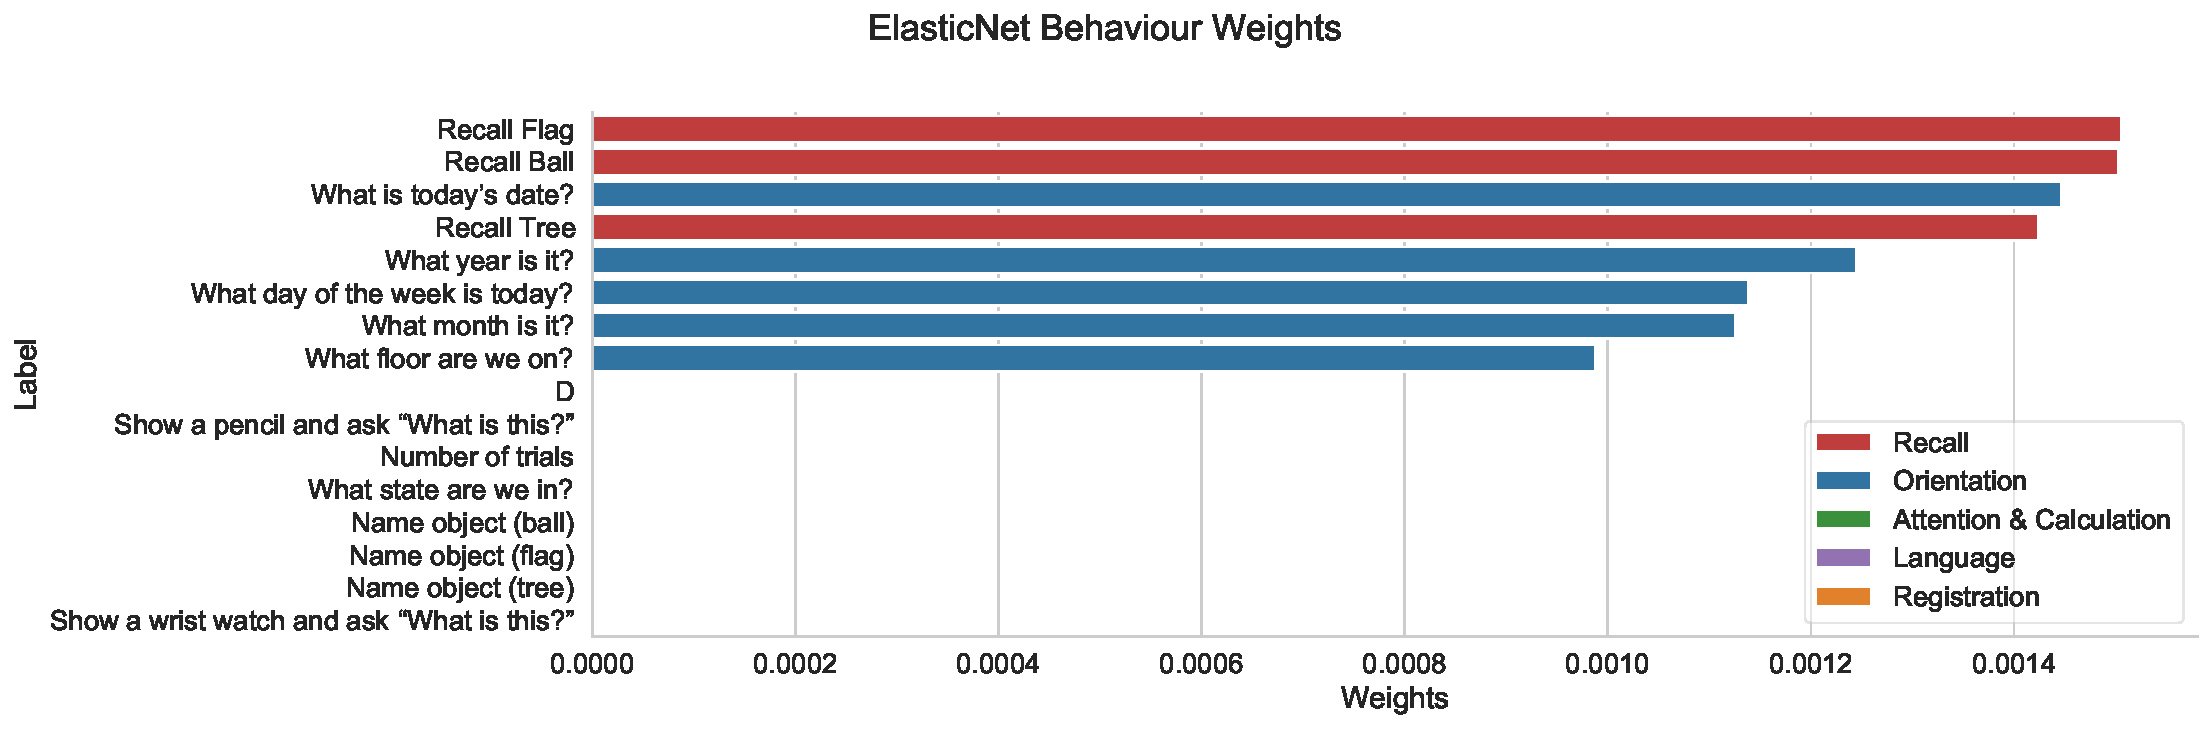
\includegraphics[width=0.8\linewidth]{figures/adni/ElasticNet behaviour weights}
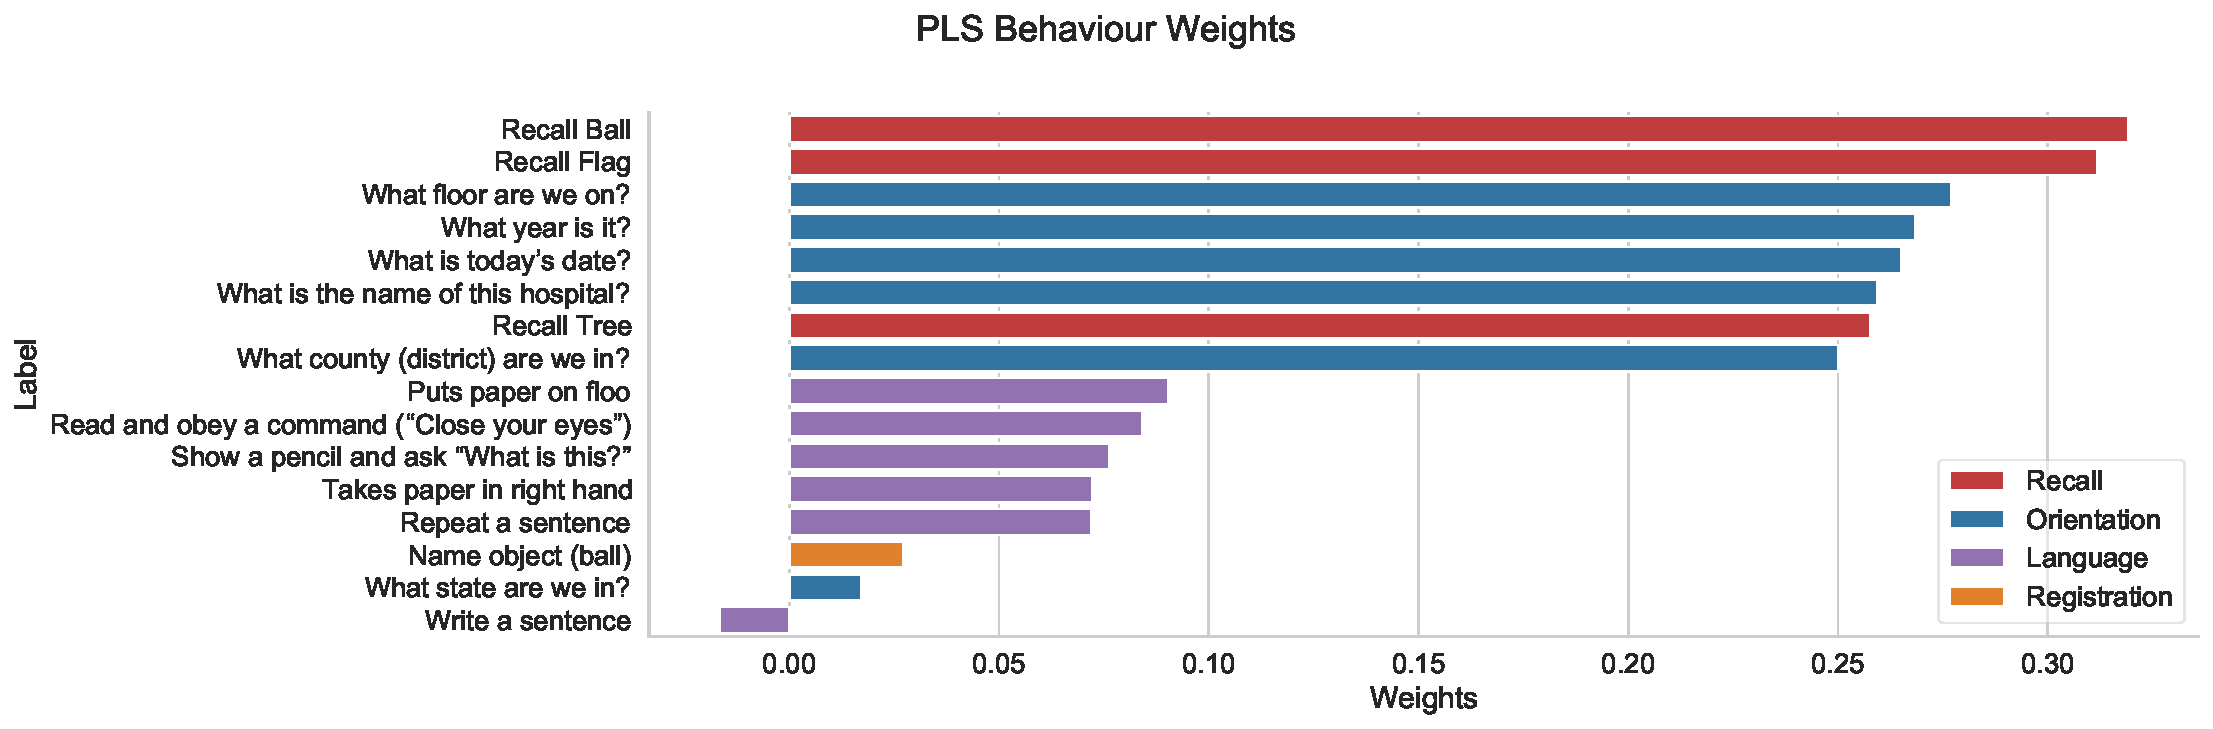
\includegraphics[width=0.8\linewidth]{figures/adni/PLS behaviour weights}
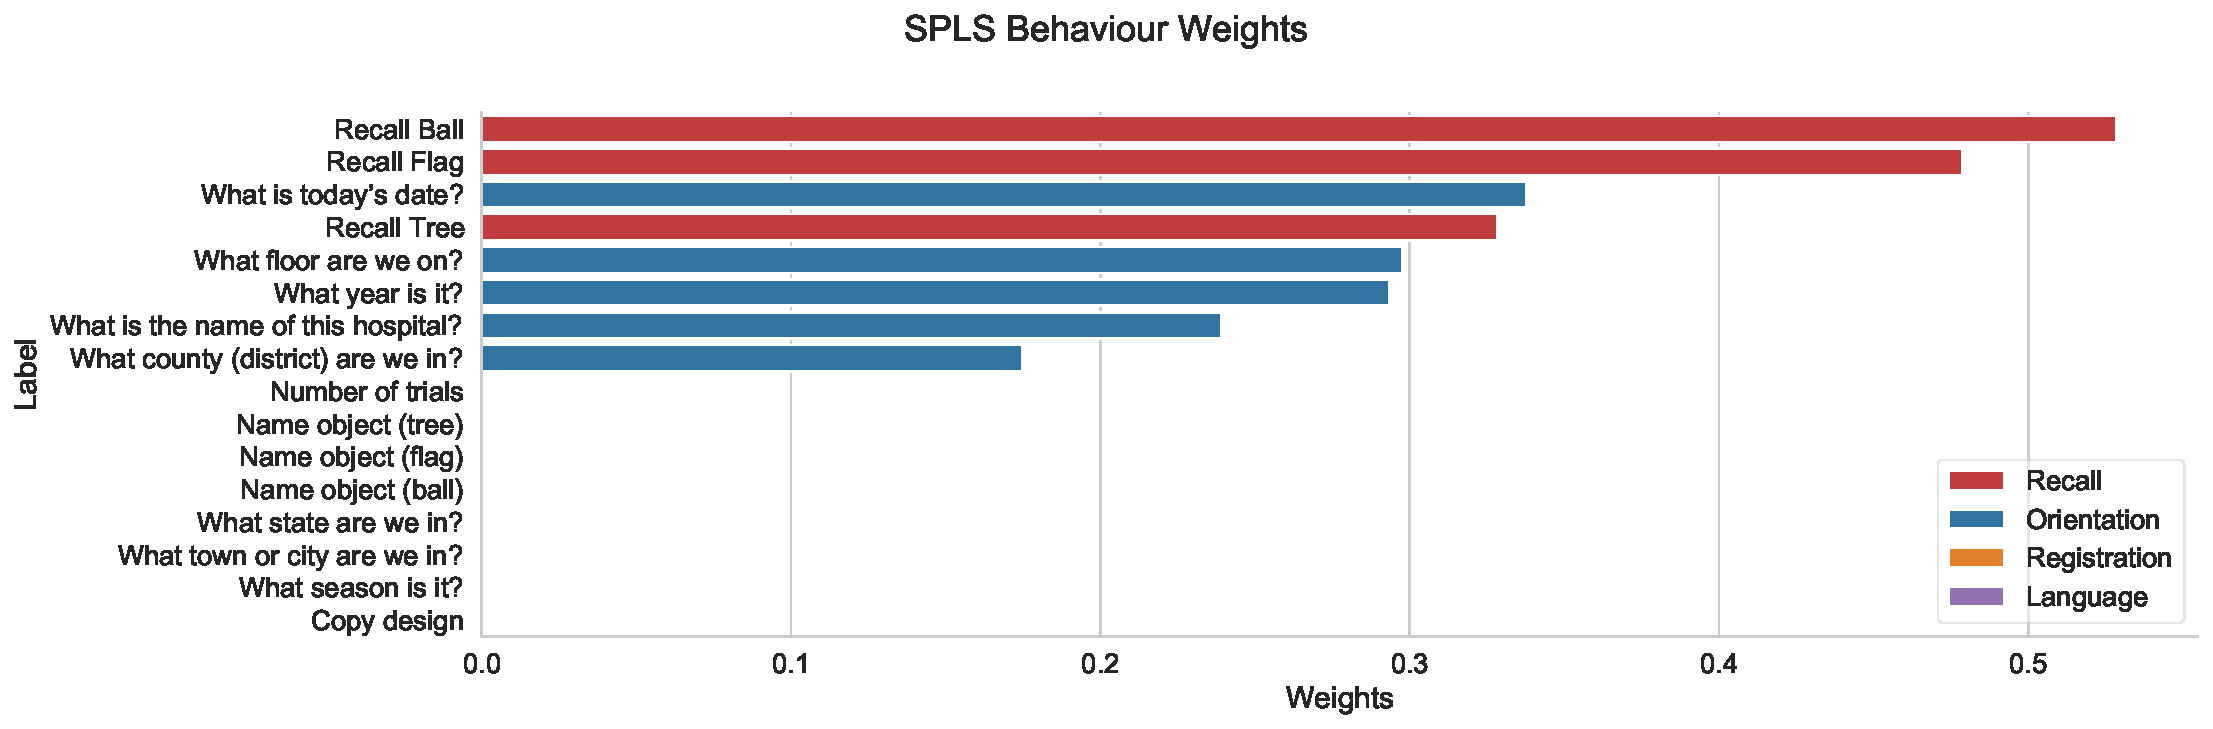
\includegraphics[width=0.8\linewidth]{figures/adni/SPLS behaviour weights}
\caption{Bar plots of the behaviour weights and loadings for each model.}\label{fig:adni-beh}
\end{figure}

\subsubsection{Brain Structure Weights and Loadings}

We plot the weights and loadings as a mosaic plot with 3 slices in each direction in Figure~\ref{fig:adni-brain}.
Previous work using SPLS with the ADNI dataset identified the same striking pattern of weights with the model strikingly selecting the hippocampal weights\cite{monteiro2016multiple}.
While the Elastic Net has a less visually appealing selection of weights, with a honeycomb pattern near the edges of the brain, the hippocampal region is more clearly loaded on in the loadings space (and likewise for RCCA).
It is noticeable that PCA, PLS and SPLS both weights in the same direction whereas RCCA and Elastic Net weight different regions with opposite signs.

\begin{figure}
\centering
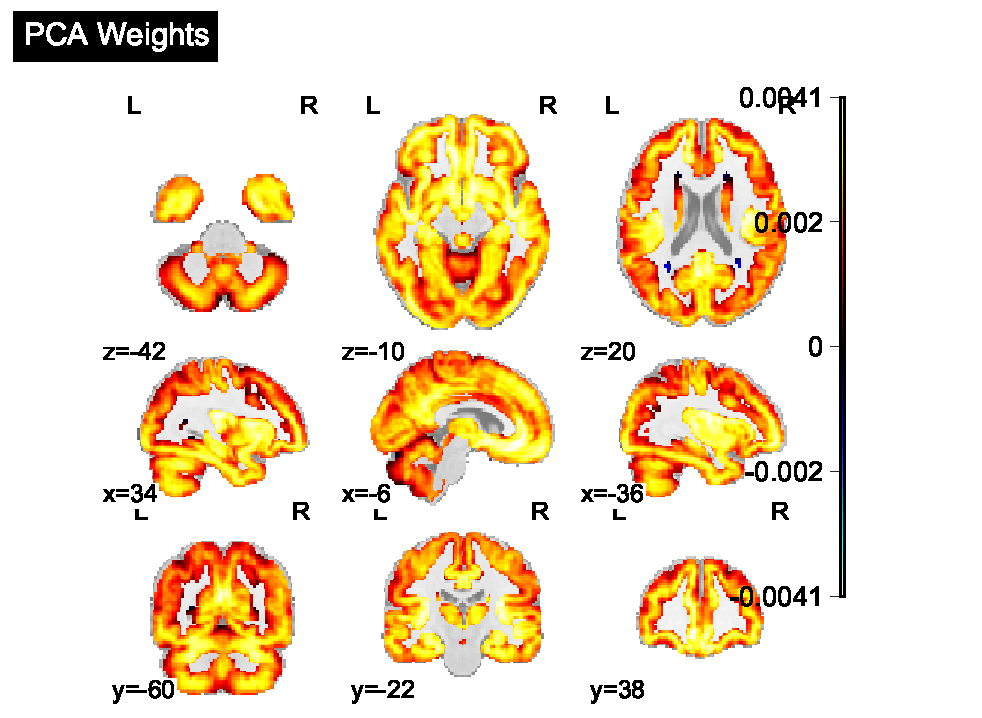
\includegraphics[width=0.45\linewidth]{figures/adni/PCA brain weights mosaic}
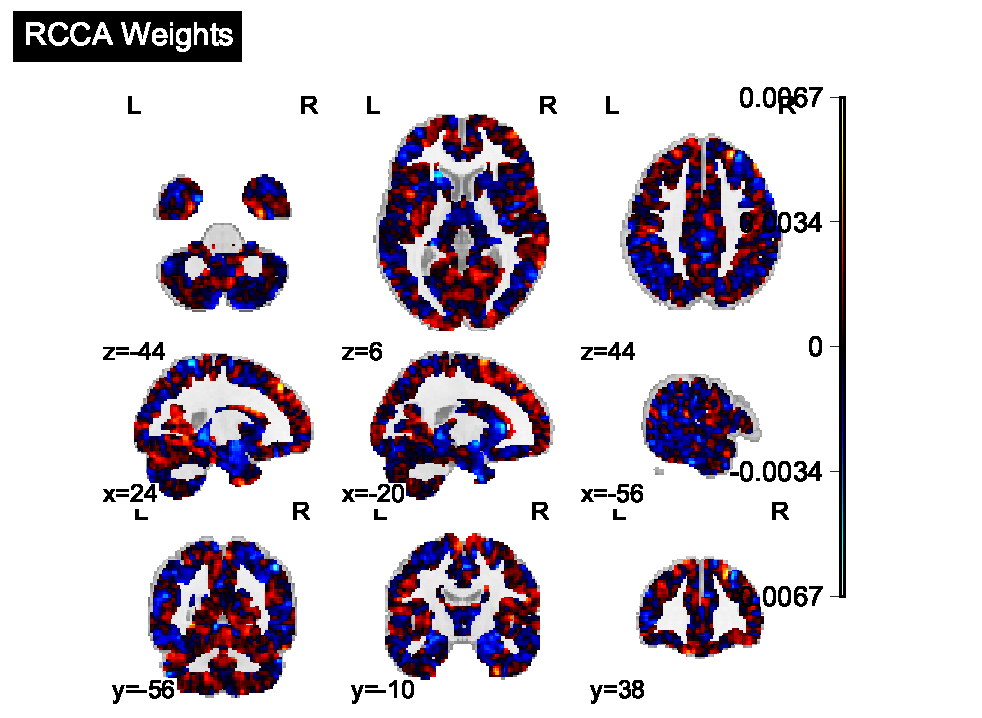
\includegraphics[width=0.45\linewidth]{figures/adni/RCCA brain weights mosaic}
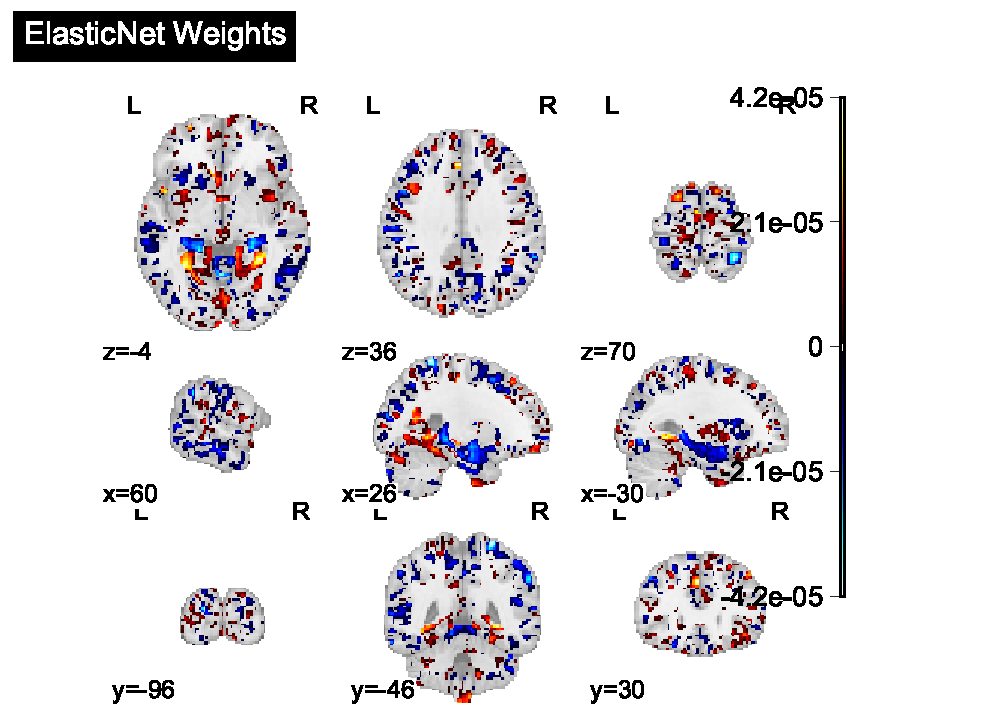
\includegraphics[width=0.45\linewidth]{figures/adni/ElasticNet brain weights mosaic}
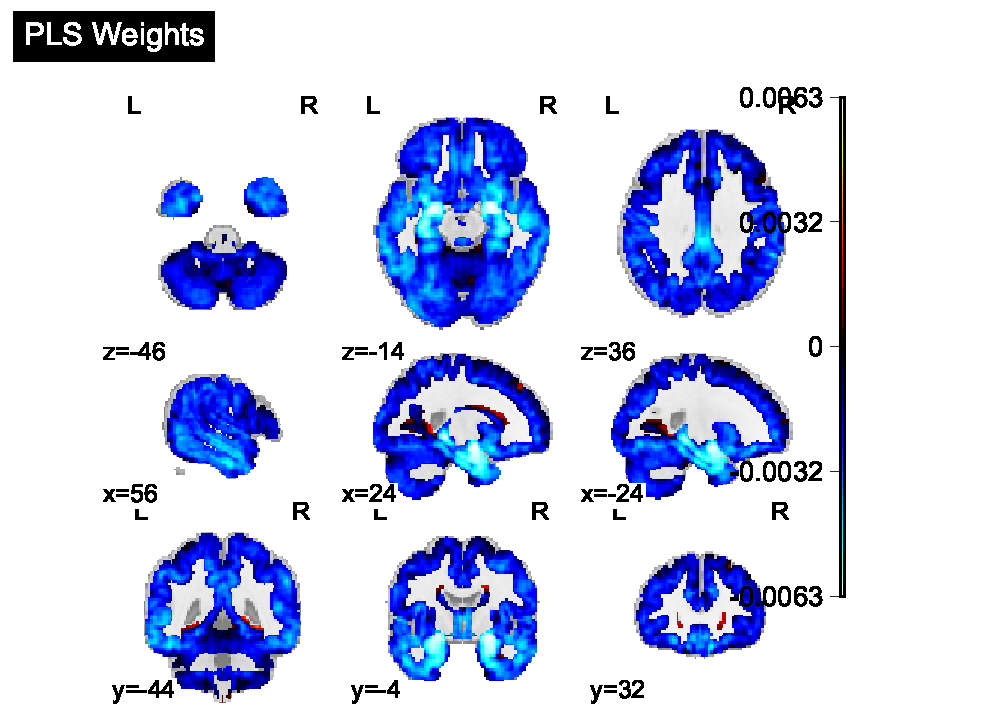
\includegraphics[width=0.45\linewidth]{figures/adni/PLS brain weights mosaic}
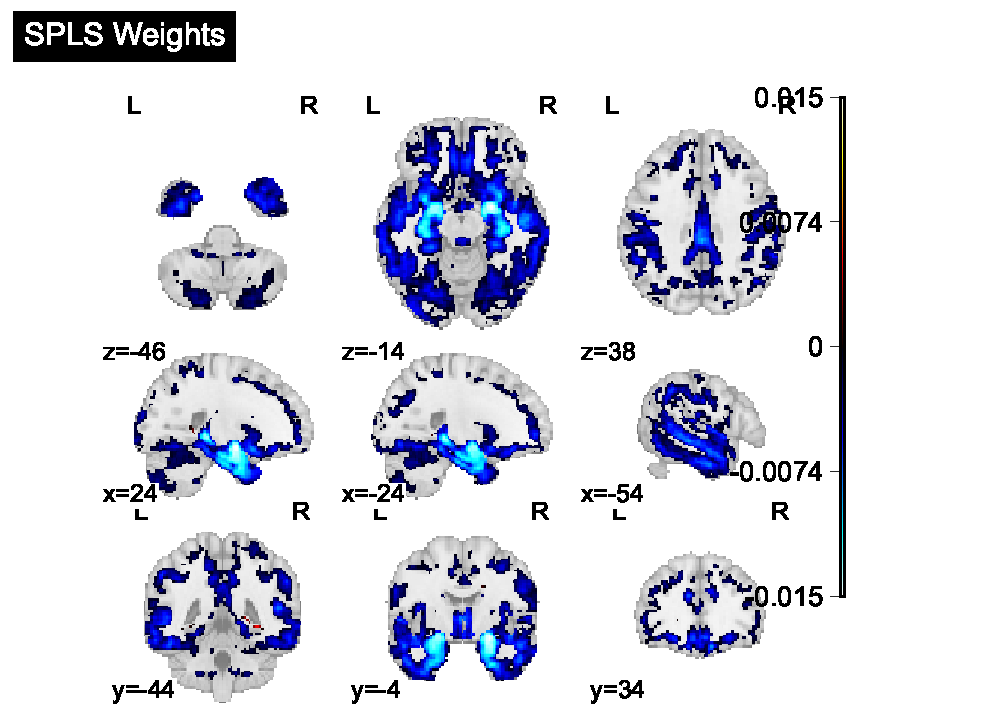
\includegraphics[width=0.45\linewidth]{figures/adni/SPLS brain weights mosaic}
\caption{Statistical maps of brain structure loadings and weights for each model.}
\end{figure}

\subsubsection{Sparsity of Weights}

Table~\ref{tab:brain-behaviour-weights-adni} once again shows the number of non-zero weights for each model.
We can see that tuned SPLS and Elastic Net once again identify sparse weights.
In this case, the difference in performance is more convincing and suggests that this sparsity is less spuriously induced than for the HCP data.
This is supported by the fact that Elastic Net and SPLS models find a similar level of sparsity in the brain weights.
On the other hand SPLS finds a much sparser set of behavioural weights.

\begin{table}[h]
\centering
\caption{Number of non-zero weights for each model.}
\begin{tabular}{|c|c|c|}
\hline
Model & Brain Weights & Behaviour Weights \\
\hline
PCA & 168130 & 31 \\
RCCA & 168130 & 31 \\
Elastic Net & 59617 & 17 \\
PLS & 168130 & 31 \\
SPLS & 74995 & 10 \\
\hline
\end{tabular}\label{tab:brain-behaviour-weights-adni}
\end{table}

\section{Discussion and Limitations}

In this section, we discuss the implications of our findings as well as the limitations of our study and the proposed FRALS method, some of which we address in later chapters of this thesis.

\subsection{Discussion}

\paragraph{Ridge CCA is typically much better than PLS across datasets:} Our results show that Ridge CCA is typically much better than PLS across datasets.
Much like regularised regression, it is unusual to need to use maximal ridge regularization even in high dimensions.
This means that while PLS might be more stable for a given dataset, it is not necessarily more stable across random samples from the same population.

\paragraph{FRALS is a useful tool for implementing Elastic Net CCA:} Our results show that FRALS is a useful tool for implementing Elastic Net CCA.

\subsection{FRALS Limitations}
While FRALS offers promising performance in terms of out-of-sample correlation, it does come with significant drawbacks, the most noteworthy being its computational inefficiency.
Below, we outline the primary factors contributing to the slow speed of FRALS and provide some insights into the computational bottlenecks.

\paragraph{Changing Regression Targets}\label{subsec:changing-regression-targets}
Adding to the computational burden is the fact that the regression targets, i.e., the projections of the other view, are not static but change dynamically throughout the algorithm's run.
Each update to the least squares solution consequently alters the global objective, leading to a constantly shifting landscape that the algorithm needs to navigate.
This also leads to a significant amount of redundant computation, as the algorithm needs to recompute the least squares solution for each view at each iteration.

\paragraph{Computational Time}\label{subsec:computational-time}

The primary bottleneck in FRALS is the computation of the least squares solution.
For each iteration of the algorithm, we need to compute the least squares solution for each view.
This is a computationally expensive operation.
It is the primary factor contributing to the slow speed of FRALS (depending on the experiment around 10 times slower than Ridge CCA).
In the next chapter, we address this bottleneck by introducing a novel algorithm based on gradient descent.

\section{Conclusion}\label{sec:conclusion}

We have also shown that FRALS can be a useful tool for brain-behaviour studies, but that it is computationally expensive.

In the next chapter,

\chapter{Regularization and the Interpretation of CCA Weights and Loadings}\label{chap:als}
\minitoc
% chktex-file 44
% chktex-file 3


\section{Introduction}\label{sec:introduction}

The application of Canonical Correlation Analysis (CCA) methods to practical problems often involves two key aspects: predicting latent variables associated with different views, and understanding the nature of the relationship between these views.
This dichotomy in goals bears resemblance to the distinction between machine learning and probabilistic or statistical approaches to the CCA problem.
Machine learning approaches prioritize (out-of-sample) prediction of latent variables for downstream tasks, while statistical approaches seek to infer the data generation process from latent variables to the observed data.
Notably, the probabilistic approach to CCA focusses on the forward model from latent variables to observed data, while the machine learning approach focusses on the inverse model from observed data to latent variables.
As a result the probabilistic CCA is parameterized by the \textit{loadings} (parameters that transform latent variables to observed data), while the machine learning approach is parameterized by \textit{weights} (parameters that transform obsevred data to latent variables).
We would ideally like to have the best possible prediction of the latent variables, while also being able to interpret the model and understand the relationship between the views.
This implies that we would like to have models which are both good at prediction and have interpretable loadings that we can use to understand the relationship between the views via the data generation process.
The importance of the loadings (associated with the `forward' model from latent variables to observed data) instead of weights (associated with the `backward' model from observed data to latent variables) for interpretability was highlighted by \cite{haufe2014interpretation} for linear models including SVM and Lasso, along with methods for transforming `backward' weights to `forward' loadings.
We contribute to this line of work by demonstrating a similar relationship between the loadings and weights of CCA models, and showing that the loadings are more interpretable than the weights.

In this chapter, we reexamine the relationship between machine learning and probabilistic CCA approaches using simulated data.
We demonstrate that these approaches are more aligned than previously thought.
While sparse regularization of CCA weights can lead to sparse estimates of generative model loadings in some conditions, it doesn't always ensure sparse loadings, especially under anisotropic noise (i.e. noise correlated between features).
Furthermore, regularization can enhance performance in low SNR scenarios, but using the PLS objective can introduce bias, emphasizing dominant principal components and overshadowing subtler correlations.

\section{Background:Generative Perspectives on CCA}\label{sec:background}

Understanding the data generation process in Canonical Correlation Analysis (CCA) and Partial Least Squares (PLS) is pivotal for many reasons.
It influences the choice of appropriate models, evaluation metrics, and sheds light on the underlying structure and dependencies between views.
Probabilistic formulations provide a principled framework to understand this process, helping us gauge the assumptions we make and the limitations these impose.

\subsection{Probabilistic CCA and GFA (Explicit Latent Variable Models}\label{subsubsec:a-probabilistic-latent-variable-perspective-on-cca}

Consider the graphical model depicted in Figure~\ref{fig:mentalhealthselfsupervised}.
It comprises two distinct views: a neuroimaging modality and a behavioral modality.
Both views are assumed to originate from a common latent variable, representing the severity of a mental health condition.
The neuroimaging modality is generated via a linear model with added noise, while the behavioral modality similarly arises from a linear model with noise.
Consequently, the brain and behavioral modalities exhibit correlation since they both derive from the same latent variable.
In a statistical sense, they are conditionally independent, given the latent variable.

\begin{figure}
    \centering
    \tikz{
        % nodes
        \node[latent, align=center, minimum size=2cm] (Z) {Severity\\z};
        %
        \node[obs, below left=of Z, minimum size=2cm, align=center] (x1) {Brain\\$x^{(1)}$};
        \node[obs, below right=of Z, minimum size=2cm, align=center] (x2) {Behaviour\\$x^{(2)}$};
        % edges
        \edge{Z} {x1}
        \edge{Z} {x2}}
    \caption[Latent Variable Model of Mental Health]{\textit{\textbf{Latent Variable Model of Mental Health:}} From this perspective the neuroimaging modality and behavioural data are both considered to have been generated with distributions conditioned on the severity of a mental health condition}\label{fig:mentalhealthselfsupervised}
\end{figure}

The distributions of the two views are given by:

\begin{align}
    z& \sim \mathcal{N}(0, I)\\
    x\sps{i} & \sim \mathcal{N}(W\sps{i} z + \mu\sps{i}, \Psi\sps{i})
\end{align}

Where \(z\) represents the latent variable (disease severity), \(x\sps{i}\) represents the $i^{\text{th}}$ view, \(W\sps{i}\) represents the model loadings, \(\mu\sps{i}\) represents the mean, and \(\Psi\sps{i}\) represents the noise covariance matrix for the $i^{\text{th}}$ view.
Notice that if it were not for the view-specific noise, the two views would be perfectly correlated subject to a linear transformation.

\citep{bach2005probabilistic} showed that the maximum likelihood solution for this model is equivalent to the solution of the CCA problem in the sense that the loadings are the same as the CCA weights multiplied by the covariance:

\begin{align}\label{eq:probabilistic-cca}
    \hat{W}\sps{i} = \Sigma_{ii} \hat{U}\sps{i} R
\end{align}

Where $R$ is an arbitrary rotation matrix and $\hat{U}\sps{i}$ is the matrix of CCA weights for the $i$th view.
This implies that for invertible covariance matrices, we can access the `true' CCA weights by multiplying the loadings by the inverse of the covariance matrix:

\begin{align}
    \hat{U}\sps{i} = \Sigma_{ii}^{-1} \hat{W}\sps{i}
\end{align}

In practice we do not have access to the covariance matrices $\Sigma_{ii}$, so we must estimate them from the data using the sample covariance matrices $\hat{\Sigma}_{ii}$.

Notice that for Identity covariance matrices, the CCA weights are the same as the loadings.
Otherwise, there is a linear transformation between the two.
For singular covariance matrices, the CCA weights are not uniquely defined.

Moreover, the mean of the posterior distribution of the latent variables is proportional to the mean of the CCA scores\citep{klami2013bayesian}.
Group Factor Analysis (GFA) is a closely related model that assumes diagonal covariance in $\Psi\sps{i}$:

\begin{align}
    z& \sim \mathcal{N}(0, I)\\
    x\sps{i} & \sim \mathcal{N}(W\sps{i} z, \sigma\sps{i}I)
\end{align}

An interesting feature of the GFA model is that as the noise level approaches zero, the marginal distribution of the views is the same as the probabilistic PCA model for each view~\citep{tipping1999probabilistic}.
This suggests that for small noise levels, we should in fact be able to recover much of the mutual information between the views by using PCA on each view separately.
For this reason, we will use and recommend PCA as a baseline in our later experiments.
Because the diagonal covariance assumption makes inference computationally cheaper, this line of work has been able to extend to incorporate sparsity on the loadings\citep{virtanen2011bayesian} as well as missing data~\citep{ferreira2022hierarchical}.

By marginalizing out the latent variables of the generative CCA and GFA models, we can write down the joint distribution of the two views:

\begin{align}
    \begin{bmatrix} X\sps{1} \\ X\sps{2} \end{bmatrix} \sim \mathcal{N} \left( \begin{bmatrix} \mu\sps{1} \\ \mu\sps{2} \end{bmatrix}, \begin{bmatrix} W\sps{1}W\spstop{1} + \Psi_1 & W\sps{1}W\spstop{2} \\ W\sps{2}W\spstop{1} & W\sps{2}W\spstop{2} + \Psi_2 \end{bmatrix} \right)
\end{align}

Importantly, this shows us that the true covariance in each view is a function of the loadings and the noise covariance matrix.
Specifically, the covariance matrix of the $i^{\text{th}}$ view is given by:

\begin{align}
    \Sigma_{ii} = W\sps{i}W\spstop{i} + \Psi_i
\end{align}

While these generative models are well-grounded in biological processes and provide a clear latent variable perspective, their application in practice is limited compared to classical CCA.
This is primarily due to their computational intensity and the need for a careful selection of priors.
Moreover, while these models can generate data with sparse loadings, generating data with sparse weights is challenging due to the dependence of CCA weights on the covariance matrices of the views.

\subsection{A Joint Covariance Matrix Perspective (Implicit Latent Variable Model)}\label{subsubsec:a-joint-covariance-matrix-perspective}

In contrast to the explicit latent variable models discussed earlier, the joint covariance matrix perspective offers an implicit approach to understanding the data generation process.
This method focuses on the covariance matrices of the views, rather than directly modeling latent variables.
A key advantage of this perspective, particularly noted in the sparse CCA literature, is its ability to generate data with sparse weights.
This is achieved by constructing the joint covariance matrix of the two views as follows:

\begin{align}\label{eq:covariance}
    \begin{bmatrix} X\sps{1} \\ X\sps{2} \end{bmatrix} \sim \mathcal{N} \left( \begin{bmatrix} 0 \\ 0 \end{bmatrix}, \begin{bmatrix} \Sigma_{11} & \Sigma_{12} \\ \Sigma_{21} & \Sigma_{22} \end{bmatrix} \right)
\end{align}

Where $\Sigma_{11}$ and $\Sigma_{22}$ are the within-view covariance matrices and $\Sigma_{12}$ and $\Sigma_{21}$ are the between-view covariance matrices.

This has the advantage of allowing us to control the within-view covariance and therefore test the methods under specific conditions.
The process was first described by Chen~\citep{chen2013sparse} and further explained by~\citep{suo2017sparse}.

We can control the true signal by setting the active variables and correlations in the between-view covariance matrices $\Sigma_{12}$ and $\Sigma_{21}$.
Specifically we construct the between-view covariance matrices as follows:

\begin{align}
    \Sigma_{12}=\sum_{k=1}^{K}\rho_k\Sigma_{11}u\sps{1}_{k}u\spstop{2}_k\Sigma_{22}
\end{align}

Where $\rho_k$ is the $k^{\text{th}}$ canonical correlation and $u\sps{i}_k$ is the $k^{\text{th}}$ column of the matrix of weights $U\sps{i}$.

We can still access the true loadings of the implied latent variable model by using the relationship in~\ref{eq:probabilistic-cca} and multiplying the weights $u\sps{i}$ by the within-view covariance matrix $\Sigma_{ii}$.

\subsection{Summary of Data Generation Methods}

\paragraph{Comparison of Joint Covariance Matrices}
To understand the distinct approaches of each data generation method, we present a comparison of their covariance structures.
This comparison highlights the differences in how these methods model the relationship within and between views.
                {
\renewcommand{\arraystretch}{2.5} % Increase the row height
\begin{table}[h]
\centering
\caption{Covariance Structures in Data Generation Methods}
\begin{tabular}{|c|c|c|c|}
\hline
\textbf{} & \textbf{Method} & \textbf{Within-view Covariance} $\boldsymbol{\Sigma_{ii}}$ & \textbf{Between-view Covariance} $\boldsymbol{\Sigma_{12}}$ \\
\hline
\multirow{2}{*}{\rotatebox[origin=c]{90}{Explicit}} & Probabilistic CCA & $W^{(i)}W^{(i)\top} + \Psi_i$ & $W^{(1)}W^{(2)\top}$ \\
\cline{2-4}
& GFA & $W^{(1)}W^{(1)\top} + \sigma^{(1)} I$ & $W^{(1)}W^{(2)\top}$ \\
\hline
\multirow{2}{*}{\rotatebox[origin=c]{90}{Implicit}} & Joint Covariance & $\Sigma_{ii}$ & $\sum_{k=1}^{K}\rho_k\Sigma_{11}u^{(1)}_{k}u^{(2)\top}_k\Sigma_{22}$ \\
\cline{2-4}
& Joint Covariance (Identity) & $I$ & $\sum_{k=1}^{K}\rho_ku^{(1)}_{k}u^{(2)\top}_k$ \\
\hline
\end{tabular}
\label{table:covariance-structures}
\end{table}
}

\paragraph{Comparison of True Weights and Loadings}
We summarize the relationship between the weights and loadings in each data generation method, distinguishing between population and sample cases.
This distinction is crucial, especially in scenarios where the population covariance matrix \( \Sigma \) is identity, but the sample covariance matrix \( \hat{\Sigma} \) is only an approximation.

\begin{table}[h]
\centering
\caption{Relationship Between Weights and Loadings in Population and Sample Cases}
\begin{tabular}{|c|c|c|c|c|}
\hline
\textbf{} & \textbf{Method} & \textbf{Case} & \textbf{Weights} & \textbf{Loadings} \\
\hline
\multirow{4}{*}{\rotatebox[origin=c]{90}{Explicit}} & Probabilistic CCA & Population & $(W^{(i)}W^{(i)\top} + \Psi_i)^{-1}W^{(i)}$ & $W^{(i)}$ \\
                          &                   & Sample & $\hat{\Sigma_{ii}}^{-1}W^{(i)}$ & $W^{(i)}$ \\
\cline{2-5}
                          & GFA & Population & $(W^{(i)}W^{(i)\top} + I)^{-1}W^{(i)}$ & $W^{(i)}$ \\
                          &     & Sample & $\hat{\Sigma_{ii}}^{-1}W^{(i)}$ & $W^{(i)}$ \\
\hline
\multirow{4}{*}{\rotatebox[origin=c]{90}{Implicit}} & Joint Covariance (Non-Identity) & Population & $U^{(i)}$ & $\Sigma_{ii}U^{(i)}$ \\
                          &                                & Sample & $U^{(i)}$ & $\hat{\Sigma_{ii}}\hat{U^{(i)}}$ \\
\cline{2-5}
                          & Joint Covariance (Identity) & Population & $U^{(i)}$ & $U^{(i)}$ \\
                          &                             & Sample & $U^{(i)}$ & $\hat{\Sigma_{ii}}\hat{U^{(i)}}$ \\
\hline
\end{tabular}
\label{tab:weights-loadings-population-sample}
\end{table}

With this comprehensive understanding of data generation methods, we now transition to examining the role of regularization in handling high-dimensional and structured data, a critical aspect in the effective application of these models.

\section{Methods}

In this section, we outline the methodologies employed in our study for Canonical Correlation Analysis (CCA) and related techniques.
We then outline our experimental design, which assesses the performance of FRALS and other CCA variants on both simulated and real datasets, aiming to understand weight and loading interpretations and the effects of regularization on model performance and clarity.
Lastly, we specify the parameters and sources of the datasets used.

\subsection{The predictive framework for CCA}\label{subsec:the-predictive-framework-for-cca}

To evaluate the performance of CCA models, we employ a standard predictive framework.
We split the data into training and test sets using a 80:20 split, and use the training set to fit the model.
We then use the test set to evaluate the model's performance.
Where relevant, pre-processing is performed on the training set and the same pre-processing is applied to the test set.
This is important to avoid data leakage, where information from the test set is used to fit the model.

\subsubsection{Model Selection}

For the models that require hyperparameter tuning, we use a grid search to find the best hyperparameters.
Specifically, we use 5-fold cross-validation to evaluate the performance of a model with a given set of hyperparameters on 5 different splits of the training data with non-overlapping validation sets.
We optimise for the hyperparameters that give the best average out of sample correlation.

\subsubsection{Model Comparisons}
We employ several CCA variants for this experiment, including Canonical Correlation Analysis (CCA), Partial Least Squares (PLS), and more.

\begin{table}[h]
\centering
\caption{Employed CCA Variants}
\begin{tabular}{|l|l|l|l|}
\hline
\textbf{Model} & \textbf{Abbreviation} & \textbf{Hyperparameters}  \\
\hline
Canonical Correlation Analysis & CCA & -   \\
\hline
Regularized CCA & RCCA & \(c_1, c_2\)   \\
\hline
Partial Least Squares & PLS & -   \\
\hline
Sparse PLS & SPLS & \(\tau_1, \tau_2\)   \\
\hline
FRALS - Elastic & Elastic & \(\alpha_1, \alpha_2, \text{l1}_1, \text{l1}_2\)   \\
\hline
Principal Component Analysis & PCA & -  \\
\hline
\end{tabular}\label{table:cca-variants}
\end{table}

\subsection{Datasets}\label{subsec:datasets}

We used 8 datasets in our experiments, including 6 simulated datasets and 2 real datasets.
The simulated datasets were generated using the methods described in section~\ref{subsec:generative-perspectives-on-cca} and the real datasets were sourced from the Human Connectome Project (HCP) and the Alzheimer's Disease Neuroimaging Initiative (ADNI).

\subsubsection{Simulated Data}

Simulated data was characterized by distinct properties, including sparse weights and/or loadings.
In our experiments, both low-dimensional (10 features per view) and high-dimensional (100 features per view) scenarios were considered.
We utilized 50 training and 50 test samples for each of 10 independent random draws from the data generation process, as detailed in table~\ref{tab:simulated-data-parameters}.

\paragraph{Joint Covariance and Sparse Weights:}
In line with the Joint Covariance method described in section~\ref{subsubsec:a-joint-covariance-matrix-perspective}, we generated data under two scenarios:
\begin{itemize}
    \item Using identity covariance matrices, aligning with the 'Implicit' latent variable model (Joint Covariance (Identity)) where true weights are equivalent to true loadings.
    \item Employing non-identity covariance matrices, consistent with the 'Implicit' latent variable model (Joint Covariance (Non-Identity)) where true weights differ from true loadings, usually resulting in non-sparse weights.
\end{itemize}
The true loadings are defined as the product of the true weights and the true population within-view covariance matrix.
For each model, we estimated model loadings using the pseudo-inverse\footnote{Defined as $A^+ = (A^\top A)^{-1} A^\top$, it inverts the closest matrix to $A$ in a least squares sense}. of the sample covariance matrix.

\paragraph{Latent Variables and Sparse Loadings:}
We generated data with sparse loadings using the Probabilistic CCA and GFA models, as outlined in section~\ref{subsubsec:a-probabilistic-latent-variable-perspective-on-cca}. Notably:
\begin{itemize}
    \item The Probabilistic CCA model, which falls under 'Explicit' latent variable models, uses random covariance matrices. Here, the true weights are estimated via the pseudo-inverse due to generally non-invertible covariance matrices.
    \item In the GFA model (also an 'Explicit' model), which employs invertible identity covariance matrices, the true weights are directly equatable to true loadings, with half of the true loadings set to zero.
\end{itemize}
The signal-to-noise ratio was calibrated to mirror the correlations observed in the Joint Covariance method, with the sum of the signal's eigenvalues being twice that of the noise.
The true weights were defined as the product of the true loadings and the inverse of the true population within-view covariance matrix.
For each model, we once again estimated model loadings using the pseudo-inverse of the sample covariance matrix.

\begin{table}
\centering
\caption{Simulated Data Parameters}
\begin{tabular}{| l | l |}
\hline
\textbf{Parameter} & \textbf{Value} \\
\hline
Number of samples (\textit{n}) & 50 train, 50 test \\
Number of features in View 1 (\textit{p}) & 10 (low-dimensional), 100 (high-dimensional) \\
Number of features in View 2 (\textit{q}) & 10 (low-dimensional), 100 (high-dimensional) \\
True Latent dimensions & 1 \\
Sparsity in View 1 & 0.5 \\
Sparsity in View 2 & 0.5 \\
\hline
\end{tabular}\label{tab:simulated-data-parameters}
\end{table}

\subsubsection{Real Data}

The real datasets employed in our experiments comprise the HCP and ADNI data.
These datasets provide insights into brain functionality and behavior from different perspectives.
We chose the HCP and the ADNI datasets based on 2 recent landmark studies and the tutorial paper this chapter is loosely related to \cite{mihalik2022canonical}.

\paragraph{The Human Connectome Project (HCP)} offers publicly available resting-state functional MRI (rs-fMRI) and non-imaging measures like demographics, psychometrics, and other behavioral measures.
Specifically, we sourced data from 1003 subjects out of the 1200-subject data release of the HCP.
This dataset is constructed using brain connectivity features of the thoroughly processed rs-fMRI data.
This processing results in 19,900 brain variables for every subject.
Additionally, there are 145 non-imaging measures employed.
Notably, nine confounding variables were regressed out from both data modalities.
Each variable was standardized for zero mean and unit variance.
More details can be found in \cite{smith2015positive, mihalik2022canonical}.
We summarize the parameters of the HCP data in table~\ref{tab:hcp-parameters}.

\begin{table}
\centering
\caption{HCP Data Parameters}
\begin{tabular}{| l | l |}
\hline
\textbf{Parameter} & \textbf{Value} \\
\hline
Number of samples (\textit{n}) & 1003 \\
Number of features in View 1 (\textit{p}) & 19900 \\
Number of features in View 2 (\textit{q}) & 145 \\
\hline
\end{tabular}\label{tab:hcp-parameters}
\end{table}

\paragraph{The ADNI} database is found at \url{adni.loni.usc.edu}.
Launched in 2003, ADNI's main objective is to assess the combination of serial MRI, PET (Positron emission tomography), biological markers, and clinical and neuropsychological assessment in tracking the progression of Mild Cognitive Impairment (MCI) and early Alzheimer’s disease.
For our experiments, we used a subset of 592 unique subjects from the ADNI. The MRI scans underwent a series of processing stages, yielding a grey matter probability map.
The Mini-Mental State Examination (MMSE) scores were employed to investigate the association with the grey matter maps.
Composed of a series of brief tasks, the MMSE evaluates various cognitive domains including memory, attention, language, and visuospatial skills.
The MMSE is a widely used test for assessing cognitive impairment.
The MMSE scores range from 0 to 30, with lower scores indicating more severe cognitive impairment.
We summarize the parameters of the ADNI data in table~\ref{tab:adni-parameters}.

\begin{table}
\centering
\caption{ADNI Data Parameters}
\begin{tabular}{| l | l |}
\hline
\textbf{Parameter} & \textbf{Value} \\
\hline
Number of samples (\textit{n}) & 592 \\
Number of features in View 1 (\textit{p}) & 168130 \\
Number of features in View 2 (\textit{q}) & 31 \\
\hline
\end{tabular}\label{tab:adni-parameters}
\end{table}

\section{Results}

In this section, we present the results of our experiments.
We begin with the results of the low and high-dimensional simulated data experiments, followed by the results of the HCP and ADNI data.

\subsection{Low-Dimensional Data}

Throughout this section, for clarity, blue signifies true zero weights and loadings, while orange indicates estimated true non-zero weights and loadings.
Consistent with the theory in the previous section, we only expect sparsity in both the true weights and loadings when the data have identity covariance matrices.
Note that because we multiply model weights by the sample covariance matrix to estimate the loadings, the estimated loadings are sometimes not sparse even when both the model weights are sparse and the true covariance matrix is identity (and likewise for the inverse).
The absolute values of the weights and loadings are plotted to compare with average values across five random draws from the distribution.

\paragraph{Implicit Latent Variables (Sparse Weights):} Elastic regularization sets true zero weights close to zero and accurately retrieves true weights in both the identity (Figure~\ref{fig:joint-identity-weights-loadings}a) and non-identity (Figure~\ref{fig:joint-identity-weights-loadings}b) scenarios.
Unregularized CCA and Ridge CCA are comparable to Elastic Net regularization but slightly worse in both scenarios (Figure \ref{fig:joint-scores})
Figure~\ref{fig:joint-identity-weights-loadings}a highlights the disparity between PLS and RCCA compared to CCA.
In particular, it is clear that the PLS and SPLS models have been skewed by the principal components.
Furthermore, the SPLS does not result in appropriate shrinkage and identifies a number of false negatives.
This is perhaps suprising because all three problems are equivalent in the population setting (due to identical view covariances).
The models diverge in a sample setting because of non-identical sample covariance matrices, underscoring the distinction between population and sample settings and the interpretation complexities in the latter.
PCA performs well in the random covariance scenario, but poorly in the identity covariance scenario.
This suggests that the random covariance scenario results in a higher signal-to-noise ratio for these parameters.

\begin{figure}
\centering
\begin{subfigure}{0.49\linewidth}
\centering
\includesvg[width=\linewidth]{figures/regularization/simulated/low/Combined_Weights_Loadings_with_Error_Bars_Identity_Covariance_joint}
\caption{Identity Covariance Matrices}
\end{subfigure}
%
\begin{subfigure}{0.49\linewidth}
\centering
\includesvg[width=\linewidth]{figures/regularization/simulated/low/Combined_Weights_Loadings_with_Error_Bars_Random_Covariance_joint}
\caption{Random Covariance Matrices}
\end{subfigure}
\caption{Weights and Loadings for Implicit Latent Variable Data Generation.}\label{fig:joint-identity-weights-loadings}
\end{figure}

\begin{figure}
\centering
\begin{subfigure}{0.49\linewidth}
\centering
\includesvg[width=\linewidth]{figures/regularization/simulated/low/Train_Test_Scores_Identity_Covariance_joint.svg}
\caption{Identity Covariance Matrices}
\end{subfigure}
%
\begin{subfigure}{0.49\linewidth}
\centering
\includesvg[width=\linewidth]{figures/regularization/simulated/low/Train_Test_Scores_Random_Covariance_joint.svg}
\caption{Random Covariance Matrices}
\end{subfigure}
\caption{Test Scores for Implicit Latent Variable Data Generation.}\label{fig:joint-scores}
\end{figure}

\paragraph{Explicit Latent Variables (Sparse Loadings):} A striking observation, though theoretically consistent, from Figure~\ref{fig:latent-variable-weights-loadings}a is that PCA almost perfectly recovers the true weights and loadings for the GFA model with identity noise covariance.
Admittedly, we have chosen a reasonably high signal-to-noise ratio for this experiment, but this nonetheless demonstrates that PCA can be a useful baseline for multiview data under an isotropic latent variable noise model.
Indeed, in the identity noise covariance scenario, all the models perform similarly (Figure~\ref{fig:latent-variable-scores}a) with the exception of CCA which appears to be unstable in this setting (Figure~\ref{fig:latent-variable-weights-loadings}a).
In the random noise covariance scenario, PCA performs poorly, and CCA now performs well (Figure~\ref{fig:latent-variable-scores}b).
Figure~\ref{fig:latent-variable-weights-loadings}b indicates that with anisotropic noise covariance, PCA no longer captures the true loadings.
There is no strong evidence that SPLS or Elastic Net regularization outperform PLS or RCCA, respectively, in this setting.
This is unsurprising because the true weights are not sparse, and so the additional sparsity constraints do not help.
However, this does illustrate that priors on weights do not translate well to priors on loadings.

\begin{figure}
\centering
\begin{subfigure}{0.49\linewidth}
\centering
\includesvg[width=\linewidth]{figures/regularization/simulated/low/Combined_Weights_Loadings_with_Error_Bars_Identity_Covariance_latent_variable}
\caption{GFA (Identity Noise)}
\end{subfigure}
%
\begin{subfigure}{0.49\linewidth}
\centering
\includesvg[width=\linewidth]{figures/regularization/simulated/low/Combined_Weights_Loadings_with_Error_Bars_Random_Covariance_latent_variable}
\caption{Probabilistic CCA (Random Noise)}
\end{subfigure}
\caption{Weights and Loadings for Explicit Latent Variable Data Generation Models.}\label{fig:latent-variable-weights-loadings}
\end{figure}

\begin{figure}
\centering
\begin{subfigure}{0.49\linewidth}
\centering
\includesvg[width=\linewidth]{figures/regularization/simulated/low/Train_Test_Scores_Identity_Covariance_latent_variable.svg}
\caption{GFA}
\end{subfigure}
%
\begin{subfigure}{0.49\linewidth}
\centering
\includesvg[width=\linewidth]{figures/regularization/simulated/low/Train_Test_Scores_Random_Covariance_latent_variable.svg}
\caption{Probabilistic CCA}
\end{subfigure}
\caption{Test Scores for Explicit Latent Variable Data Generation Models.}\label{fig:latent-variable-scores}
\end{figure}

\paragraph{Measuring the Identitiness of the Covariance Matrices}

The theory we developed in section~\ref{subsec:generative-perspectives-on-cca} suggests that the identitiness of the covariance matrices is crucial for understanding how imposing sparsity on the weights imposes a prior belief in sparsity on the more biologically interesting loadings.
We can measure the identitiness of the covariance matrices by looking at the eigenvalues of the covariance matrices.
If the eigenvalues of the sample covariance matrix are all close to 1, then the sample covariance matrix is close to identity.
Departures from 1 indicate that the sample covariance matrix is not close to identity and imply multicollinearity in the data.

In the simulated data, we can see that the data generation models with identity noise covariance matrices, have eigenvalues closer to one than (Figure~\ref{fig:covariance-eigenvalues-simulated-low}).
On the other hand, these plots (shown for 10 random samples) show that all of the sample covariance matrices depart from the ideal case, \textit{even when the true covariance matrices are identity}.

\begin{figure}
\centering
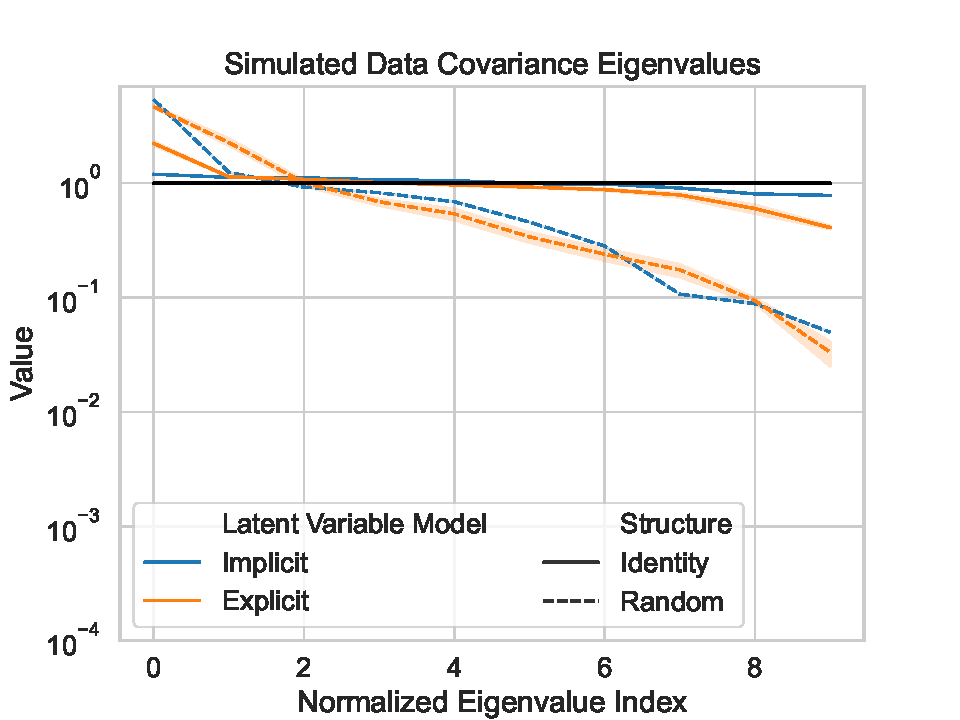
\includegraphics[width=0.8\linewidth]{figures/regularization/covariance/simulated_covariance_eigenvalues_low}
\caption{Eigenvalues of the covariance matrices for the simulated datasets.}\label{fig:covariance-eigenvalues-simulated-low}
\end{figure}

\subsection{High-Dimensional Simulated Data}
In this section we consider only the latent variable models in order to ensure we have a sufficient signal-to-noise ratio to compare the models as we are deliberately undersampled.
Figure~\ref{fig:latent-variable-weights-loadings-high}a once again shows that PCA is a useful baseline for multiview data under an isotropic noise model, even in the high-dimensional setting.
On the other hand, CCA cannot recover any signal when it is overparameterized.
Ridge CCA and PLS perform similarly, perhaps because the only identifiable signal is the PLS signal (since the CCA signal is not identifiable).
Figure~\ref{fig:latent-variable-weights-loadings-high}b illustrates clearly that both RCCA and ElasticNet with their tunable L2 regularization both outperform PLS and SPLS with fixed and maximal L2 regularization.
It appears that in high dimensions correlated noise is a significant problem for PLS (and therefore SPLS) when used as regularized CCA models, even though the models are identifiable.

\begin{figure}
\centering
\begin{subfigure}{0.49\linewidth}
\centering
\includesvg[width=\linewidth]{figures/regularization/simulated/high/Combined_Weights_Loadings_with_Error_Bars_Identity_Covariance_latent_variable}
\caption{Identity Covariance Latent Variable}
\end{subfigure}
%
\begin{subfigure}{0.49\linewidth}
\centering
\includesvg[width=\linewidth]{figures/regularization/simulated/high/Combined_Weights_Loadings_with_Error_Bars_Random_Covariance_latent_variable}
\caption{Random Covariance Latent Variable}
\end{subfigure}
\caption{Weights and Loadings for High-Dimensional Explicit Latent Variable Data Generation.}\label{fig:latent-variable-weights-loadings-high}
\end{figure}

\begin{figure}
\centering
\begin{subfigure}{0.49\linewidth}
\centering
\includesvg[width=\linewidth]{figures/regularization/simulated/high/Train_Test_Scores_Identity_Covariance_latent_variable.svg}
\caption{}
\end{subfigure}
%
\begin{subfigure}{0.49\linewidth}
\centering
\includesvg[width=\linewidth]{figures/regularization/simulated/high/Train_Test_Scores_Random_Covariance_latent_variable.svg}
\caption{}
\end{subfigure}
\caption{Test Scores for High-Dimensional Explicit Latent Variable Data Generation Models.}\label{fig:latent-variable-scores-high}
\end{figure}

%\paragraph{Identitiness of the Covariance Matrices}
%
%As in the low-dimensional case, we can measure the identitiness of the covariance matrices by looking at the eigenvalues of the covariance matrices.
%
%\begin{figure}
%\centering
%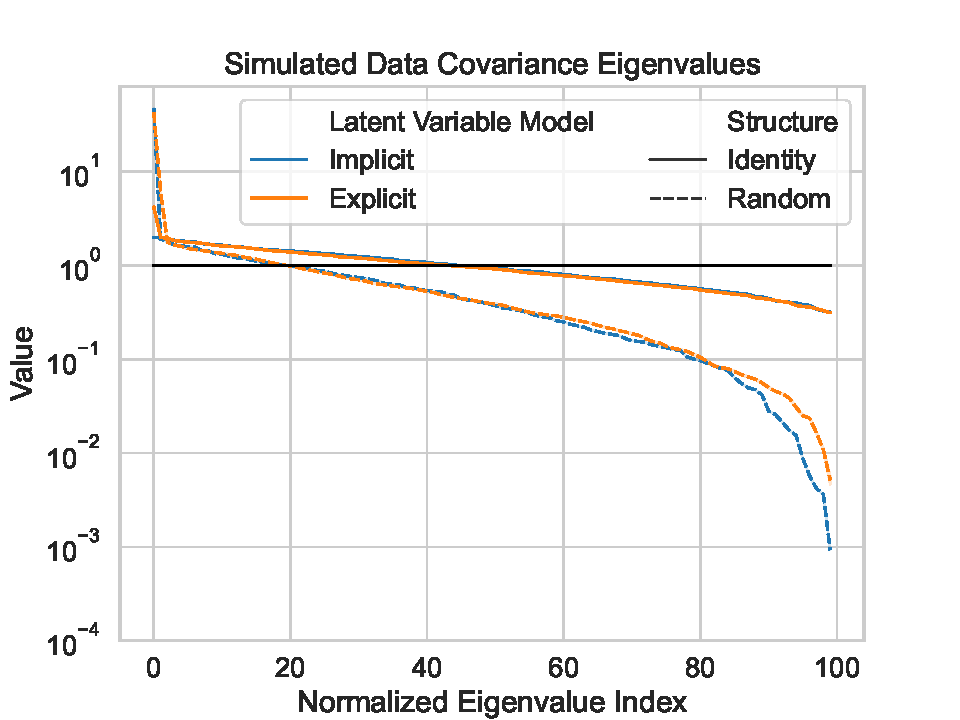
\includegraphics[width=0.8\linewidth]{figures/regularization/covariance/simulated_covariance_eigenvalues_high}
%\caption{Eigenvalues of the covariance matrices for the simulated datasets.}\label{fig:covariance-eigenvalues-simulated-high}
%\end{figure}

\newpage
\subsection{Human Connectome Project (HCP) Data}

Next, we consider the results of applying the various CCA variants to the HCP data.
Since the HCP data is high-dimensional, we drop CCA from the analysis since it would produce random results.

\subsubsection{Out of Sample Correlation}

The Elastic Net did not improve upon Ridge CCA in terms of holdout correlation captured (Figure~\ref{fig:performance}).
However, both Ridge CCA and ElasticNet outperformed PLS and SPLS.
This suggests that tunable L2 regularization is important, even for very high-dimensional data.
SPLS does however outperform PLS.

\begin{figure}
\centering
\includegraphics[width=0.5\linewidth]{figures/regularization/hcp/holdout_correlations}
\caption{Out-of-sample canonical correlations for each model.}
\end{figure}

\subsubsection{Behaviour Weights and Loadings}

Figure\ref{fig:behaviour} plots the top 8 positive and negative non-imaging loadings and their associated weights for each model\footnote{This can and does mean for example that a zero weight may have a non-zero loading!}.
This is to illustrate some of the effects we have observed in the previous section.
PCA finds a mode of variation in the behavioural data that is positively correlated with psychiatric and life function tests and negatively correlated with a number of emotion and personality tests.
The RCCA and ElasticNet models find a mode of variation in the behavioural data that is negatively correlated with the Line Orientation test and to a lesser extent smoking and positively correlated with a number of other cognitive tests.
The PLS model finds a mode of variation in the behavioural data that is somewhat similar to the `good-bad' mode in\cite{smith2015positive} with a positive correlation with agreeableness, vocabulary tests, and feelings about ones' life and a strong negative correlation with smoking, rule-breaking, and antisocial personality traits.
The SPLS mode is similar but selects out the rule-breaking and antisocial personality traits in favour of the vocabulary tests and smoking.

\begin{figure}
\centering
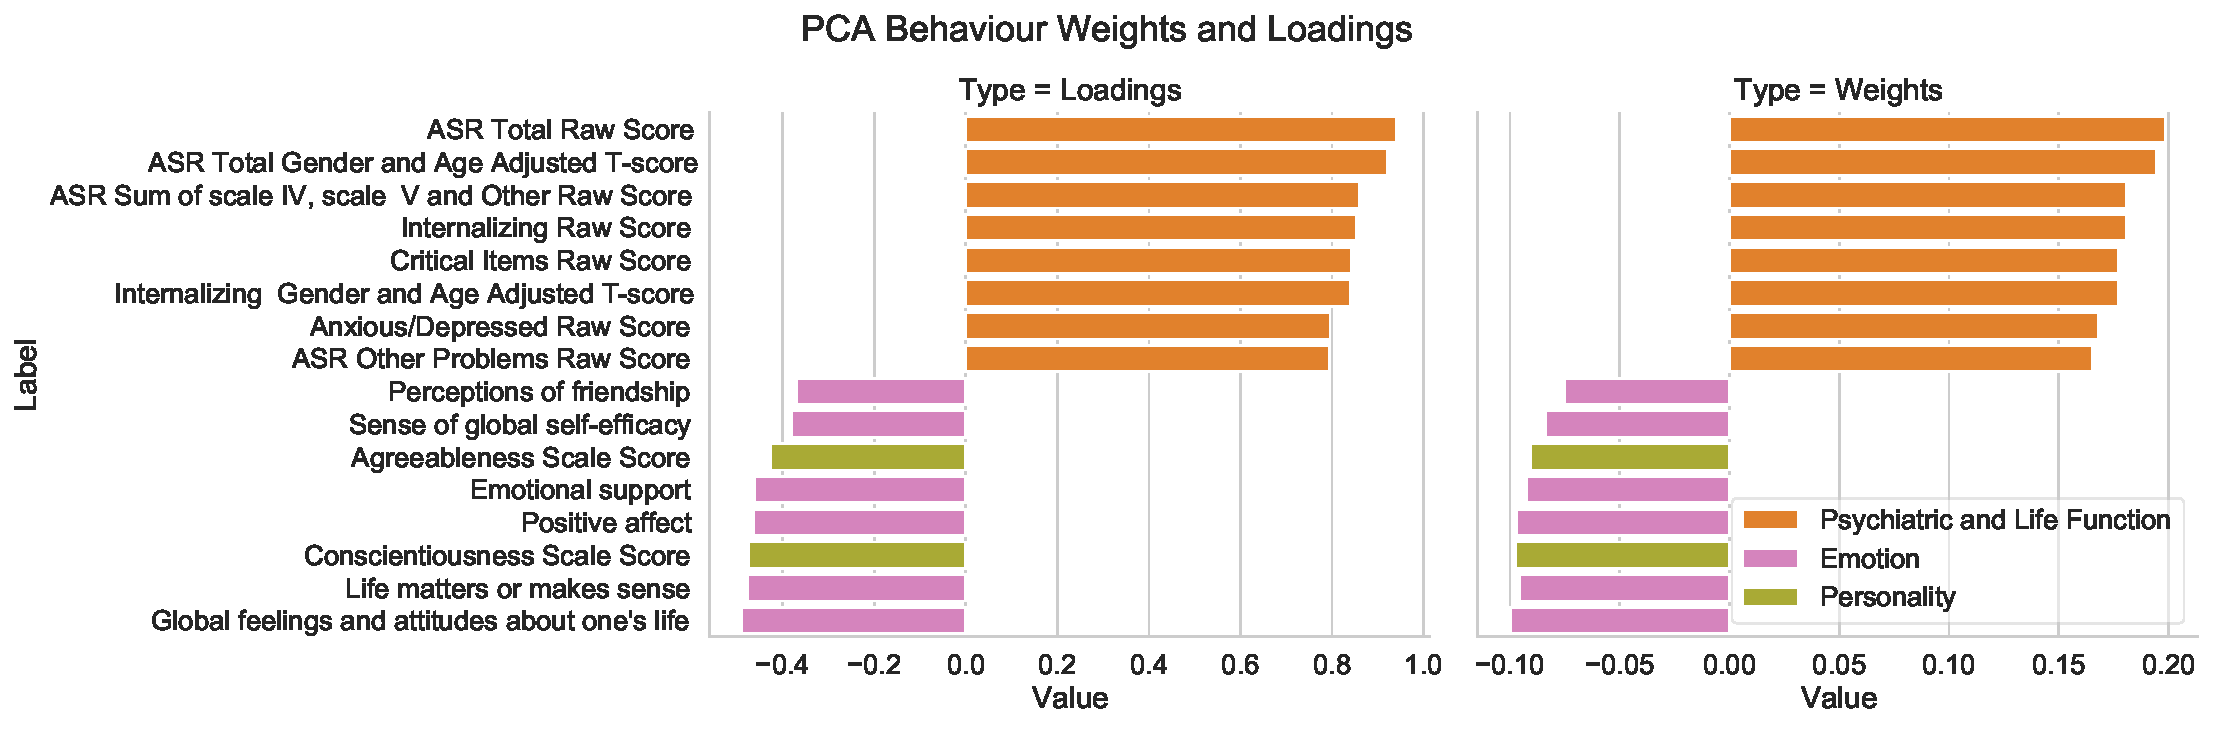
\includegraphics[width=0.8\linewidth]{figures/regularization/hcp/PCA behaviour weights and loadings}
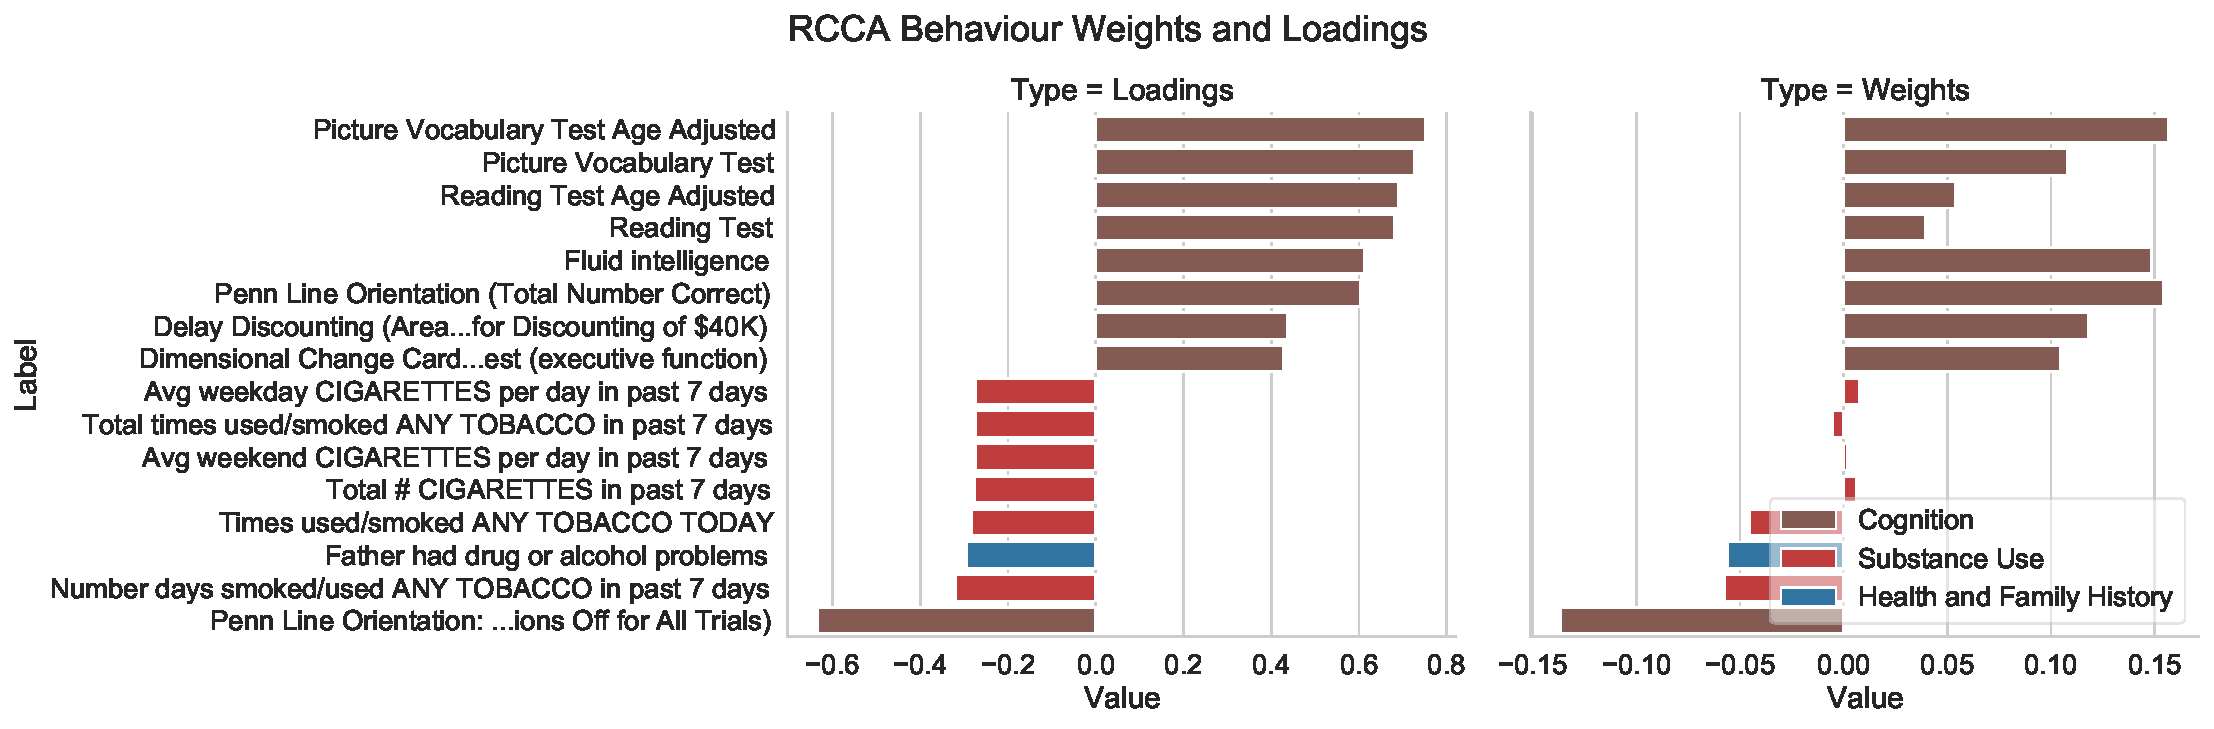
\includegraphics[width=0.8\linewidth]{figures/regularization/hcp/RCCA behaviour weights and loadings}
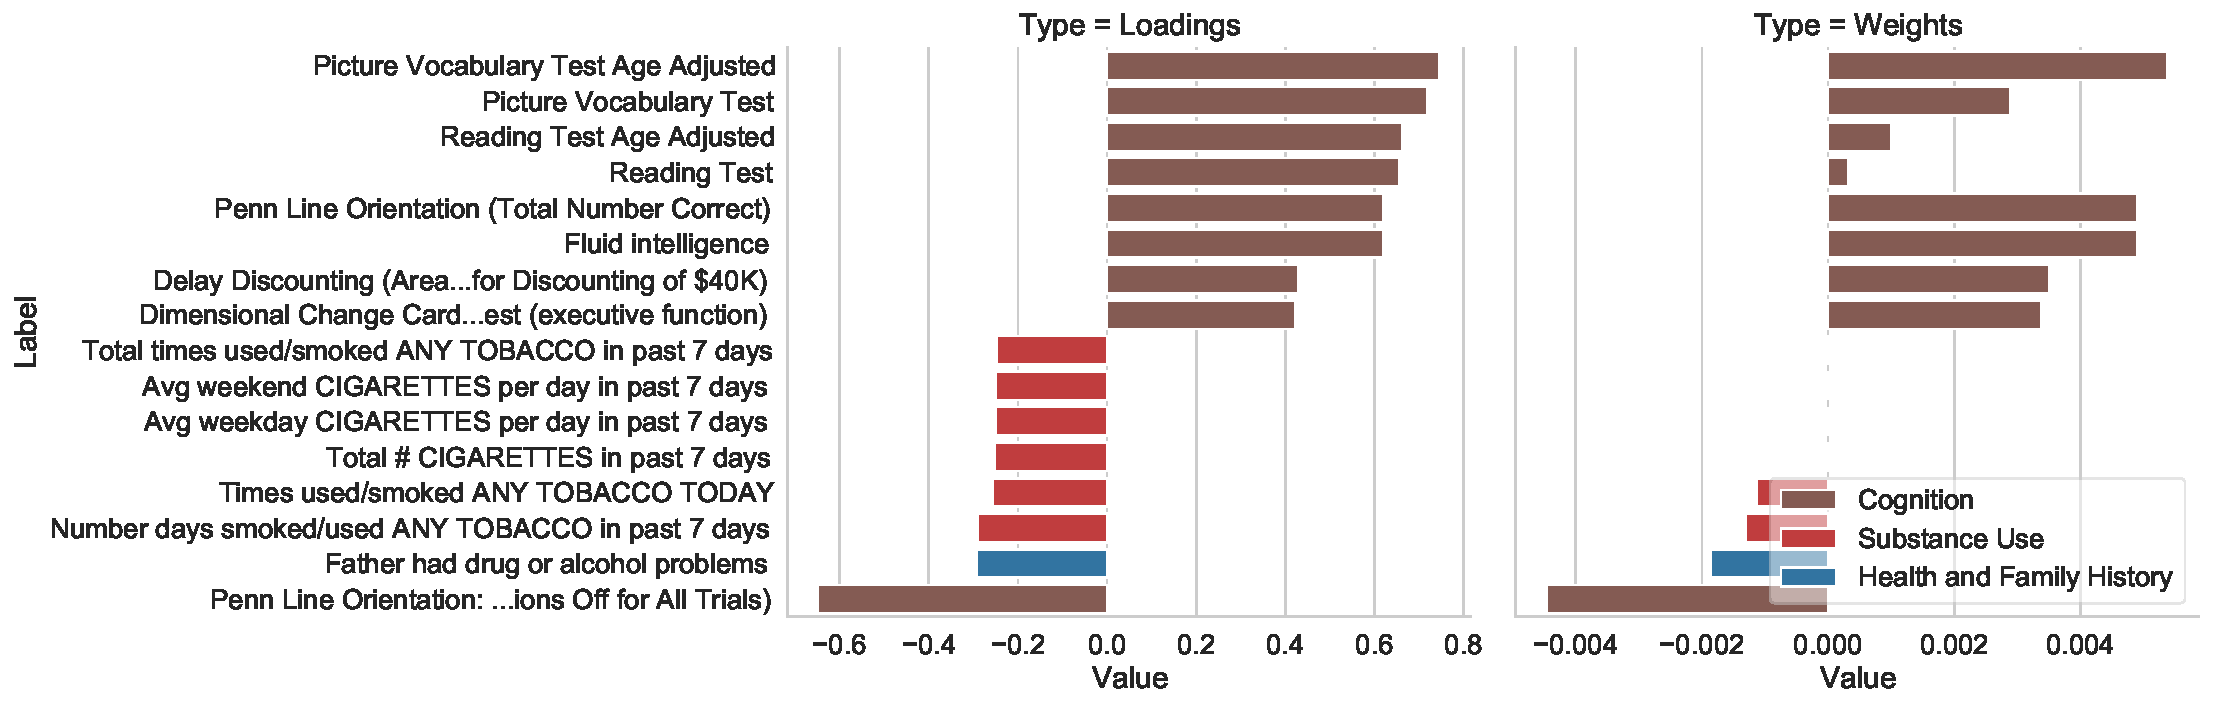
\includegraphics[width=0.8\linewidth]{figures/regularization/hcp/ElasticNet behaviour weights and loadings}
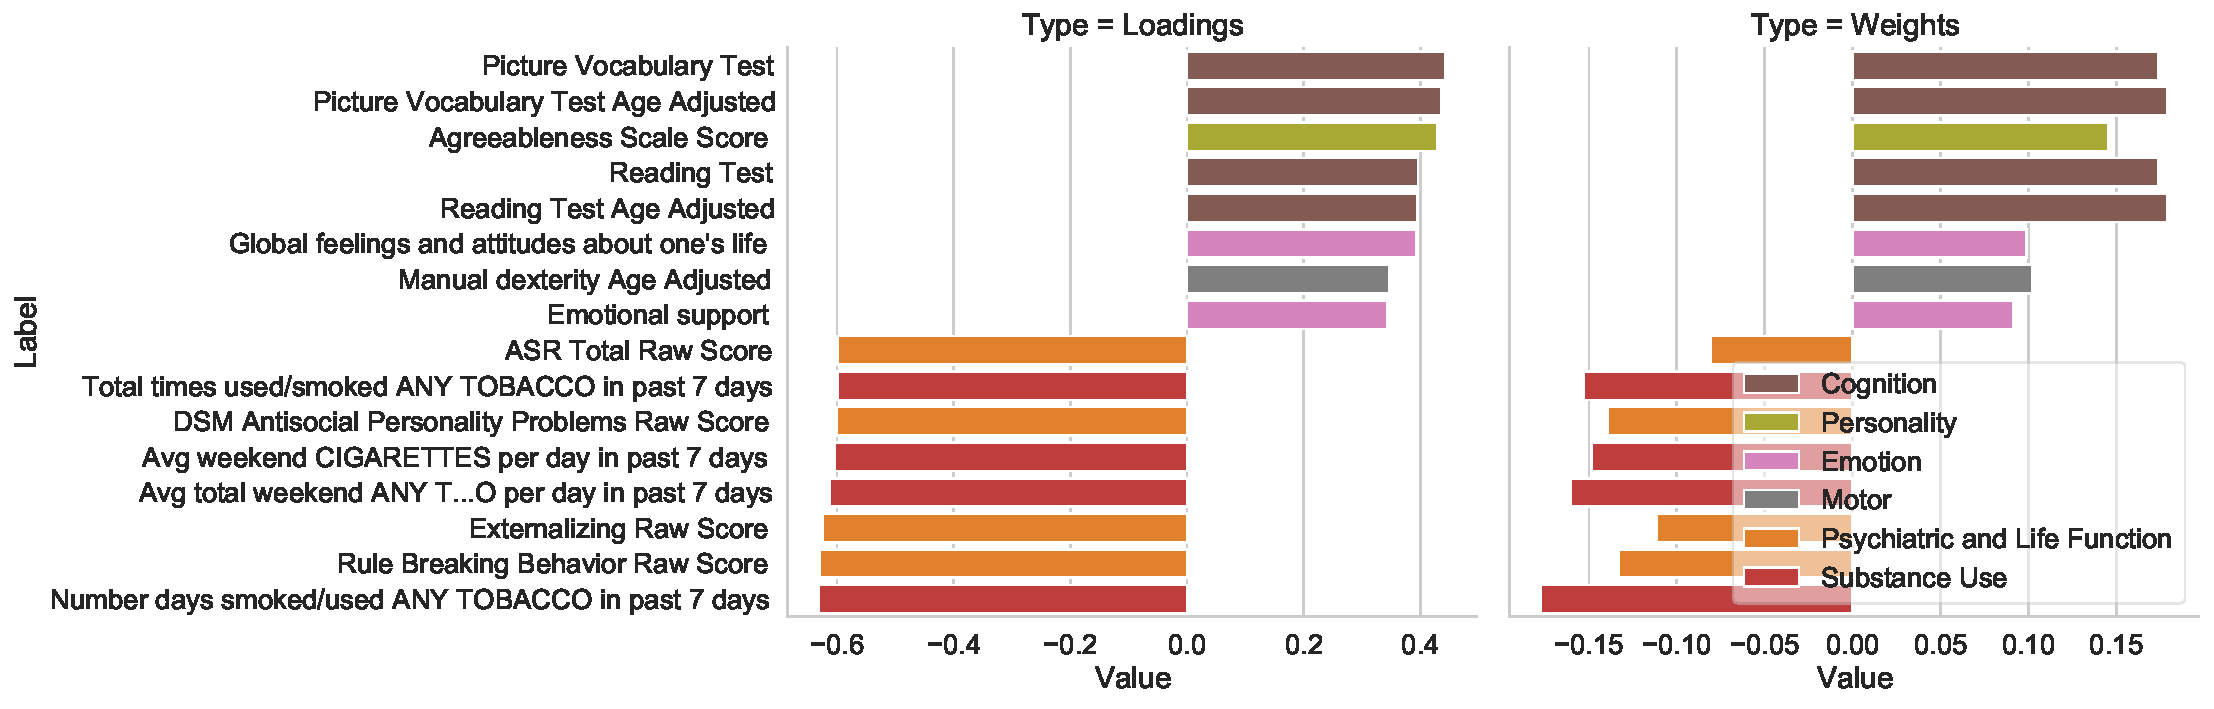
\includegraphics[width=0.8\linewidth]{figures/regularization/hcp/PLS behaviour weights and loadings}
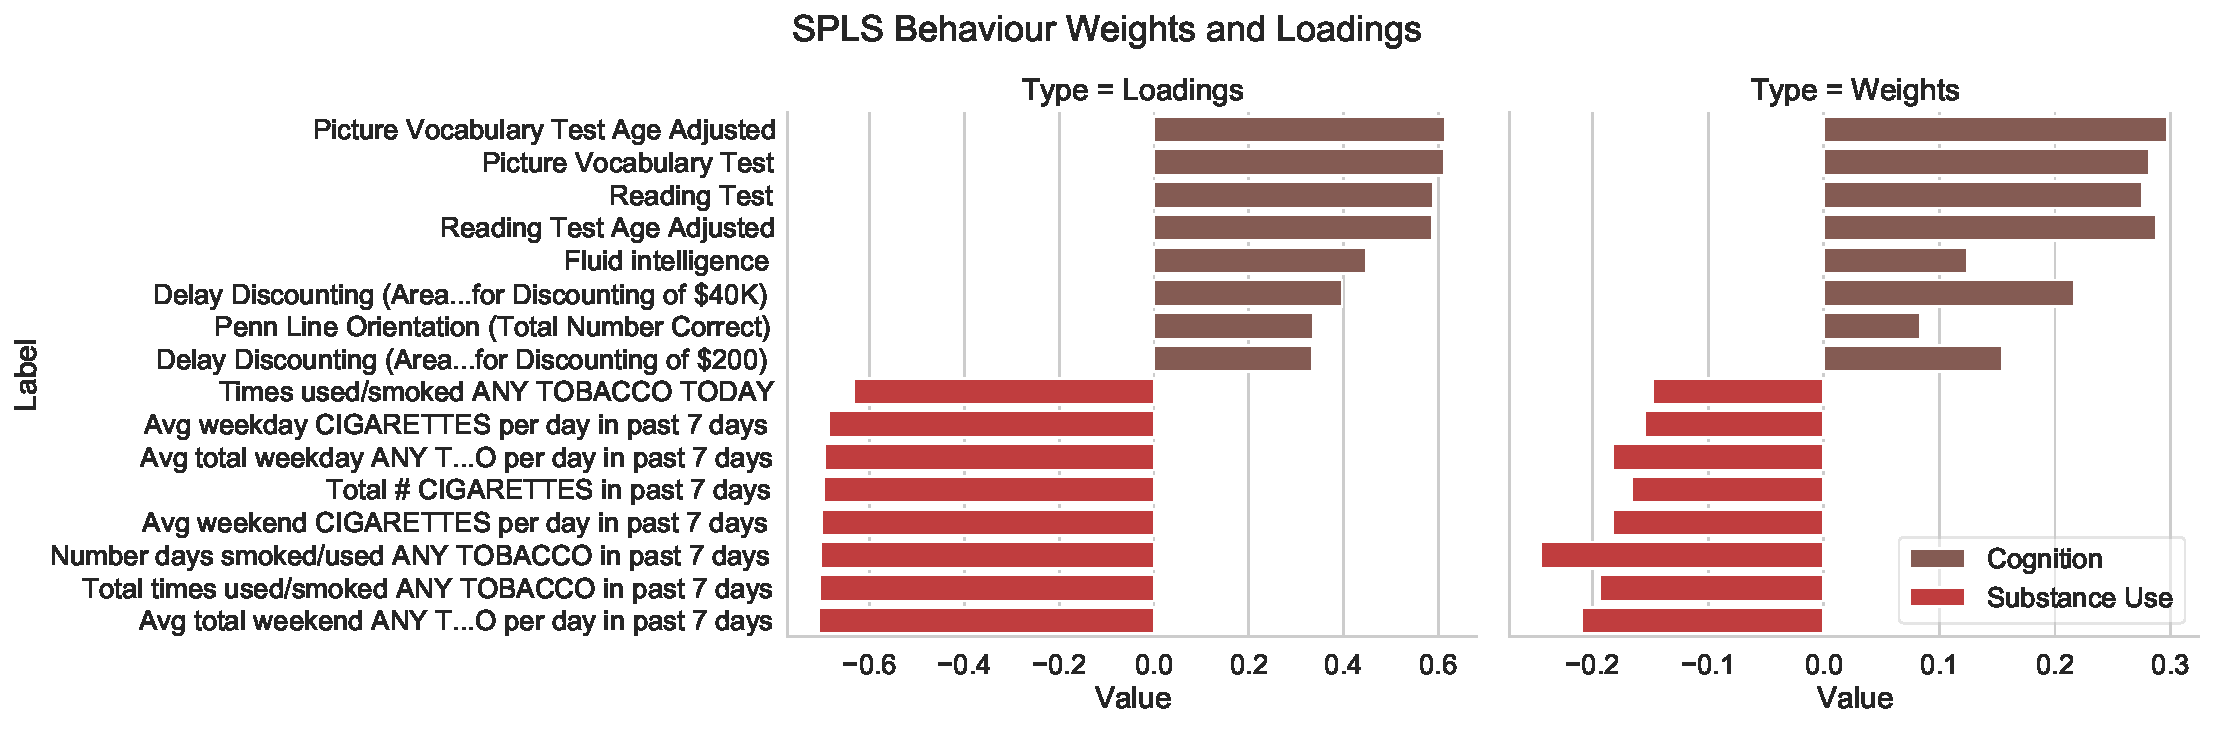
\includegraphics[width=0.8\linewidth]{figures/regularization/hcp/SPLS behaviour weights and loadings}
\caption{Top 8 positive and negative non-imaging loadings for each model}\label{fig:behaviour}
\end{figure}

\subsubsection{Brain Connectivity Weights and Loadings}

In this section, we use two different methods to visualize the brain connectivity weights and loadings.
The first method is to use chord diagrams to visualize the top 8 positive and negative brain weights and loadings for each model.
This approach is inspired by the chord diagrams used in \cite{smith2015positive}.
The second method is to use surface maps to visualize the brain connectivity weights and loadings.
This approach has been used by both \cite{ferreira2022hierarchical} and \cite{smith2015positive}.

\paragraph{Chord Diagrams}
We grouped the nodes of the connectivity matrix of our data into 7 parcels according to the Yeo 7 network parcellation\cite{yeo2011organization}.
These are then arranged around the circumference of the chord diagram using the Nichord package\cite{bogdan2023connsearch}.
The plots then show the 8 strongest positive and negative weights or loadings for each model as `chords'.
The chord diagrams in Figure~\ref{fig:chord_weights} and Figure~\ref{fig:chord_loadings} show the top 8 positive and negative brain weights and loadings for each model.

\textcolor{red} Need to find something biologically useful to say about these.

\begin{figure}
\centering
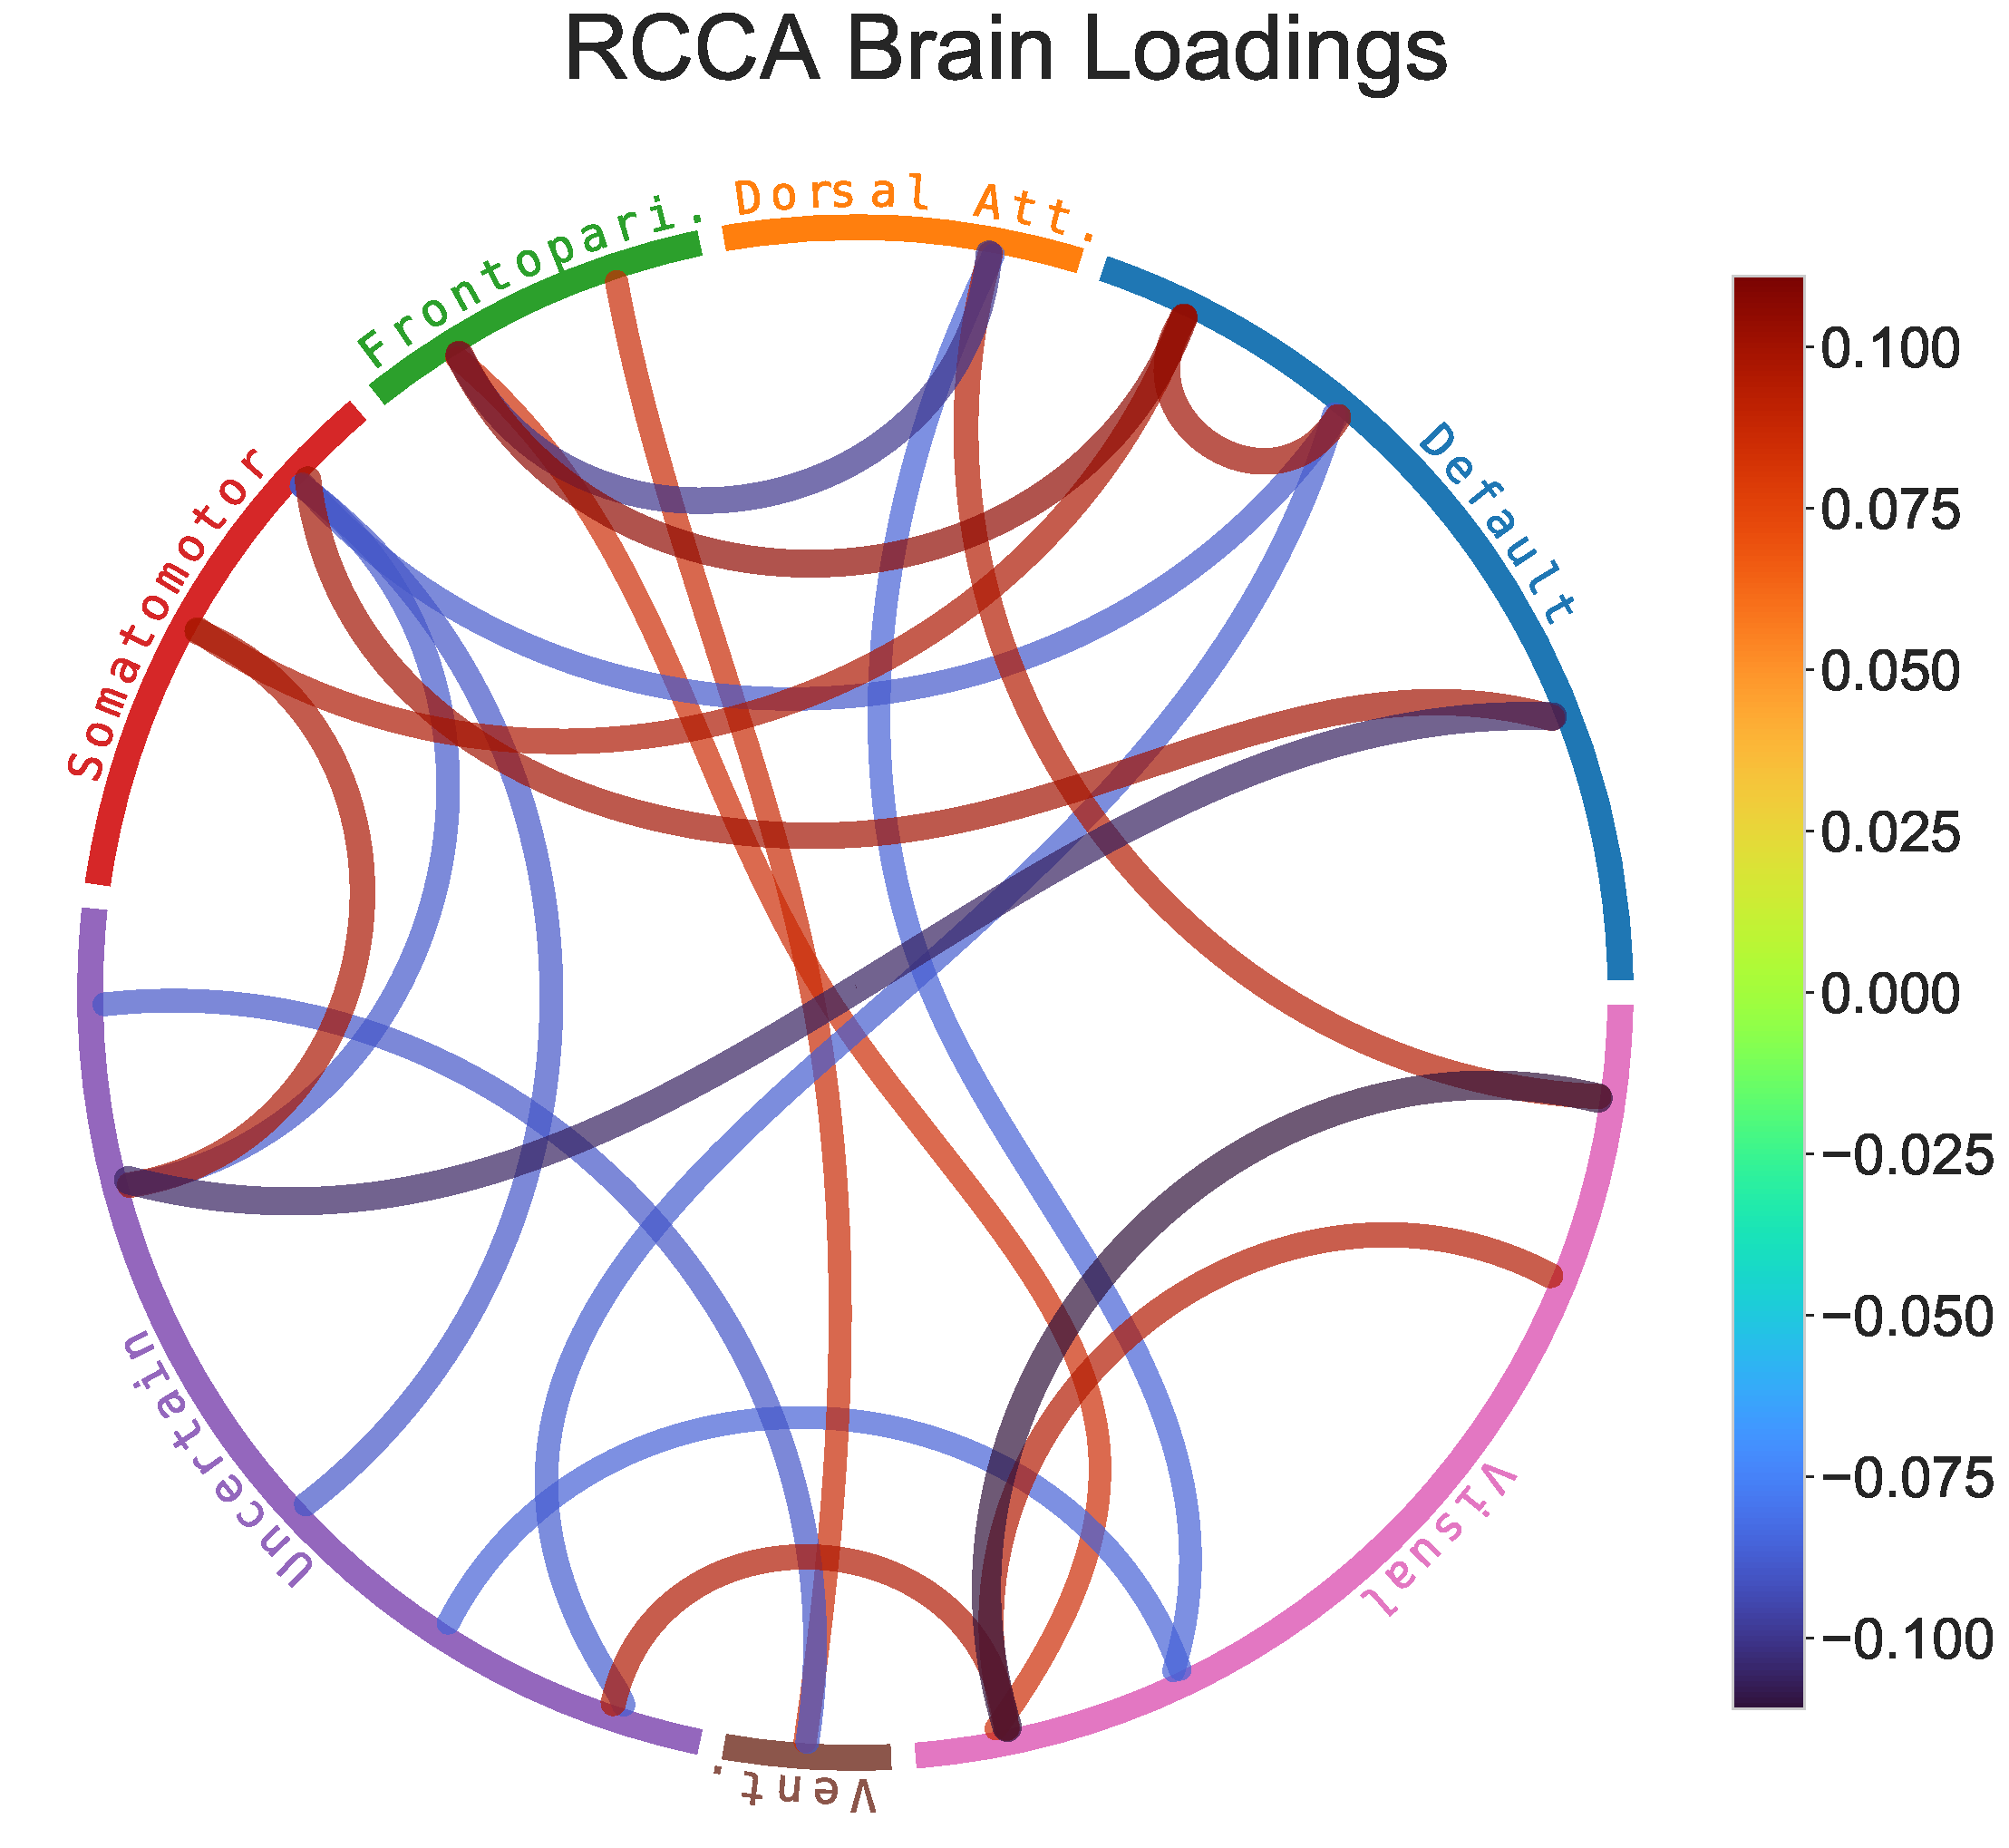
\includegraphics[width=0.49\linewidth]{figures/regularization/hcp/RCCA brain weights}
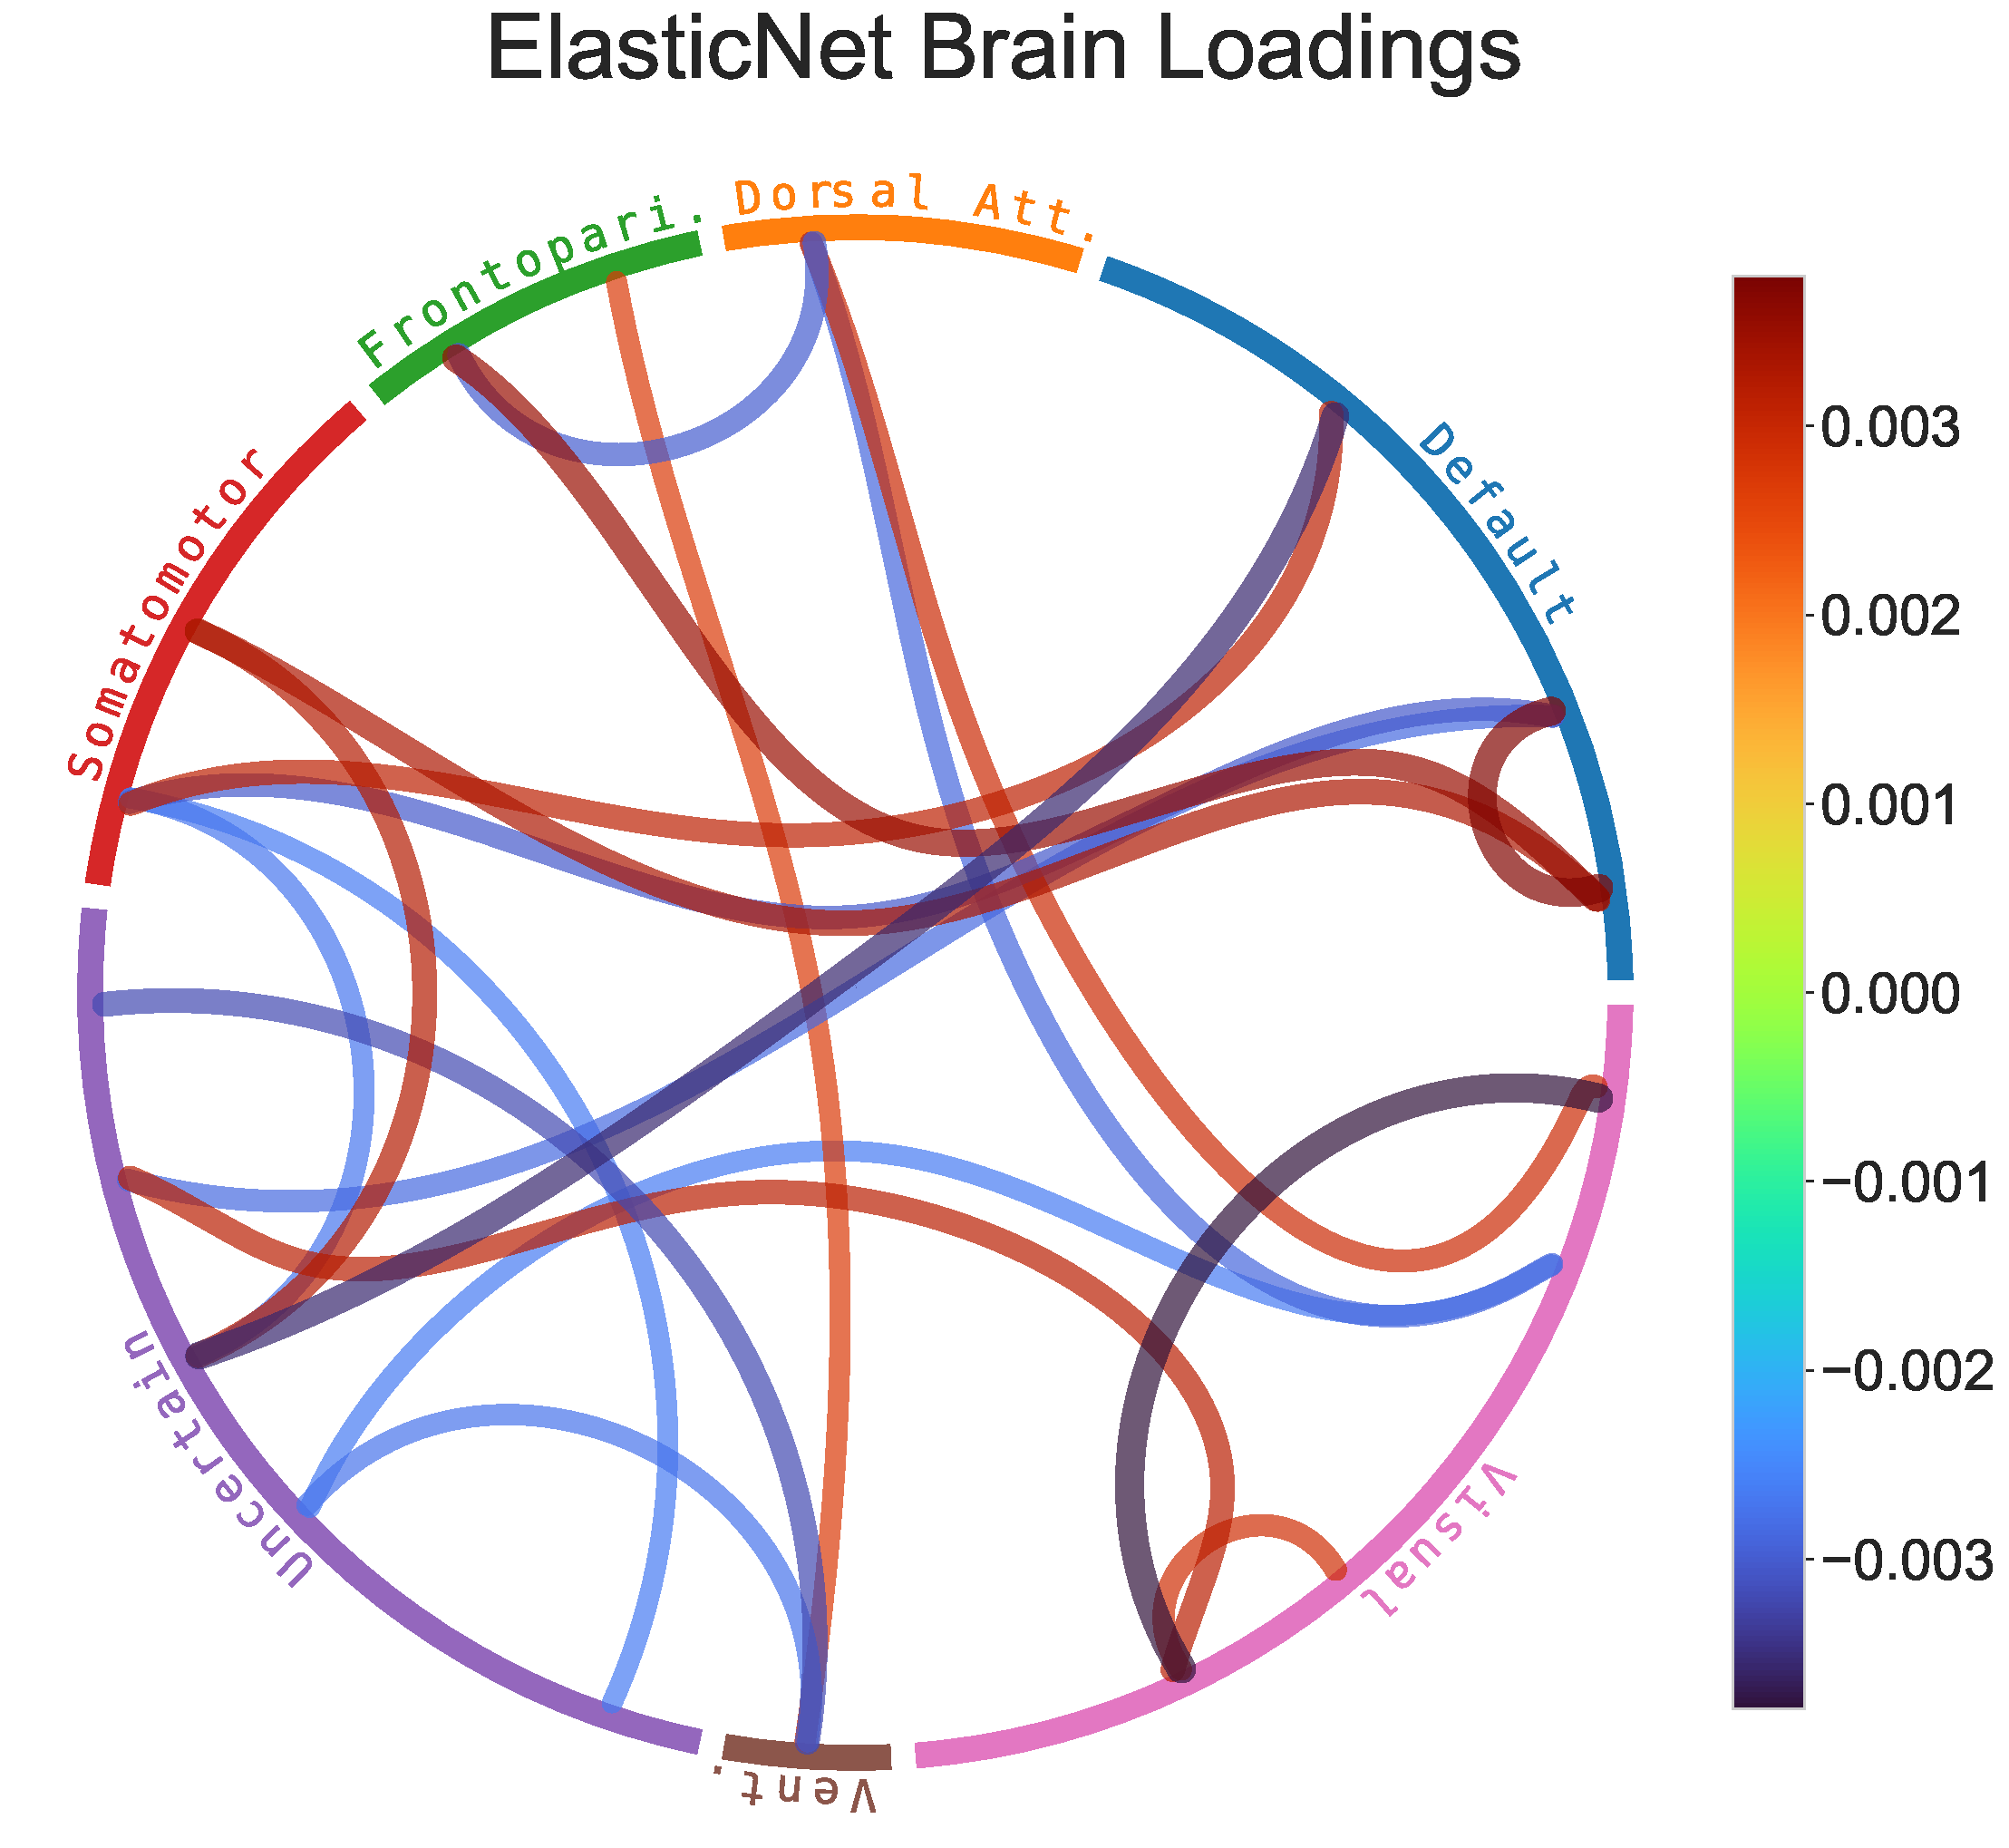
\includegraphics[width=0.49\linewidth]{figures/regularization/hcp/ElasticNet brain weights}
\includegraphics[width=0.49\linewidth]{figures/regularization/hcp/PLS brain weights}
\includegraphics[width=0.49\linewidth]{figures/regularization/hcp/SPLS brain weights}
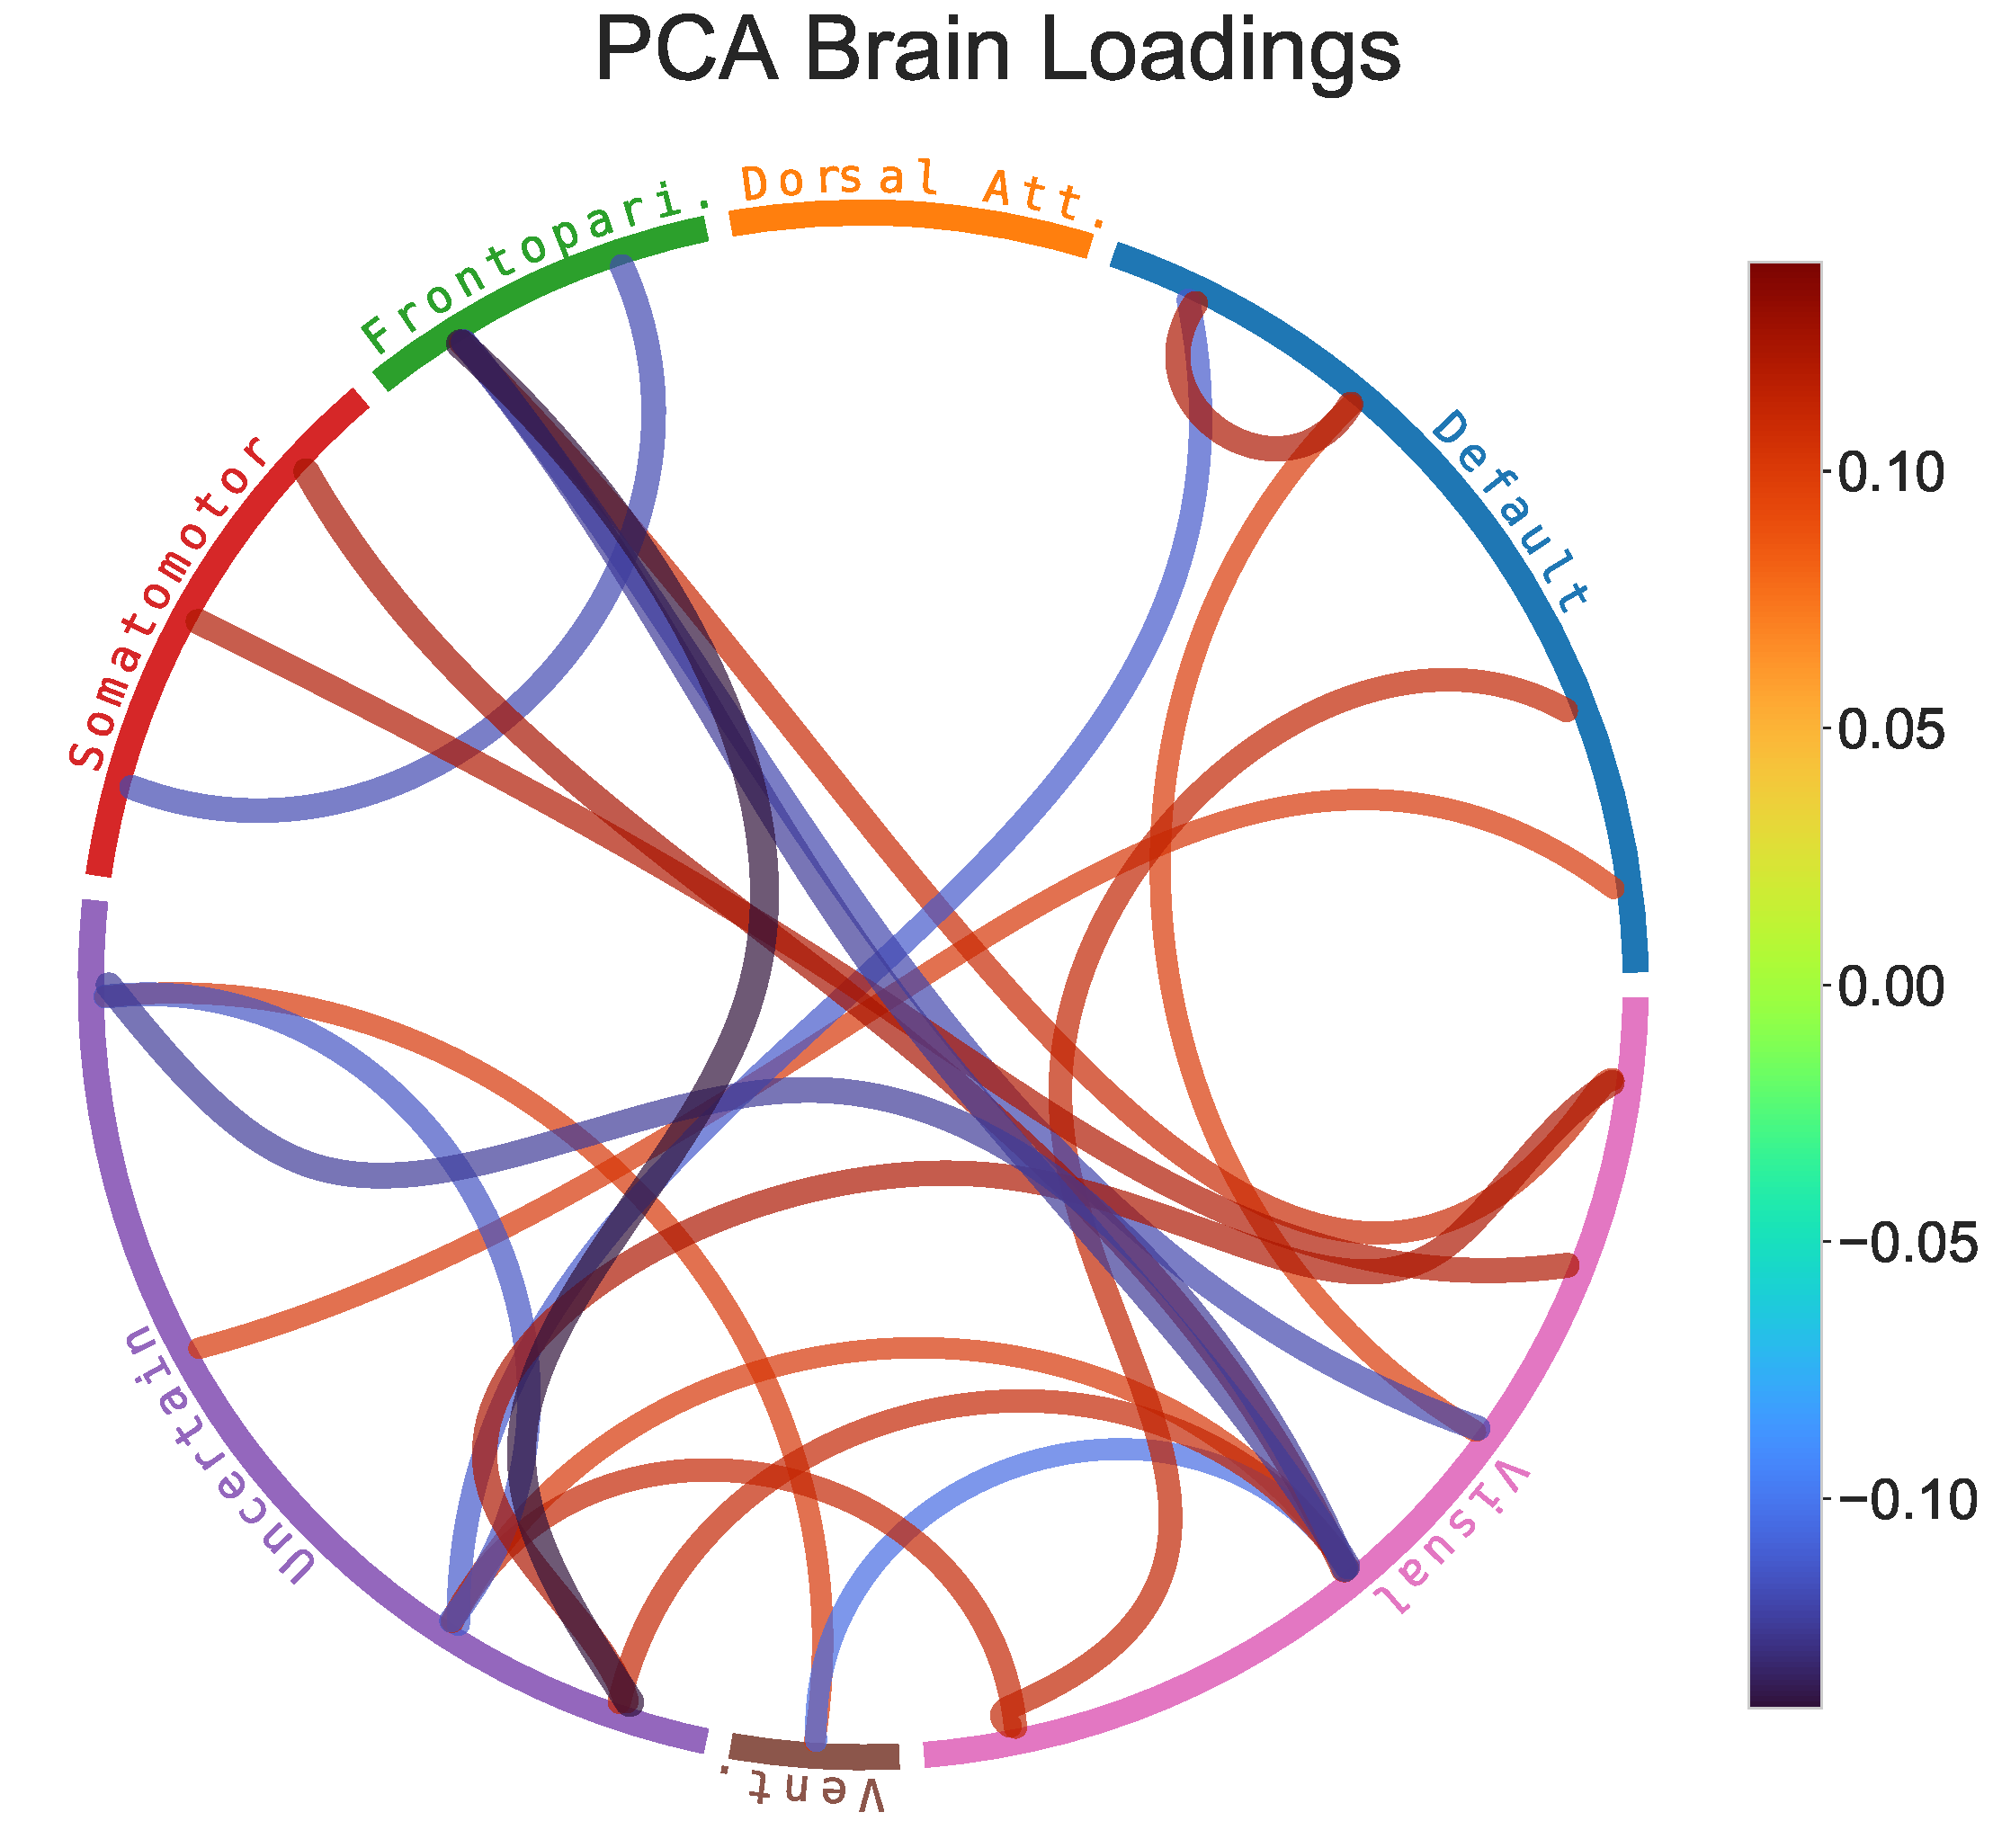
\includegraphics[width=0.49\linewidth]{figures/regularization/hcp/PCA brain weights}
\caption{Chord diagrams of the top 8 positive and negative brain weights for each model.}\label{fig:chord_weights}
\end{figure}

\begin{figure}
\centering
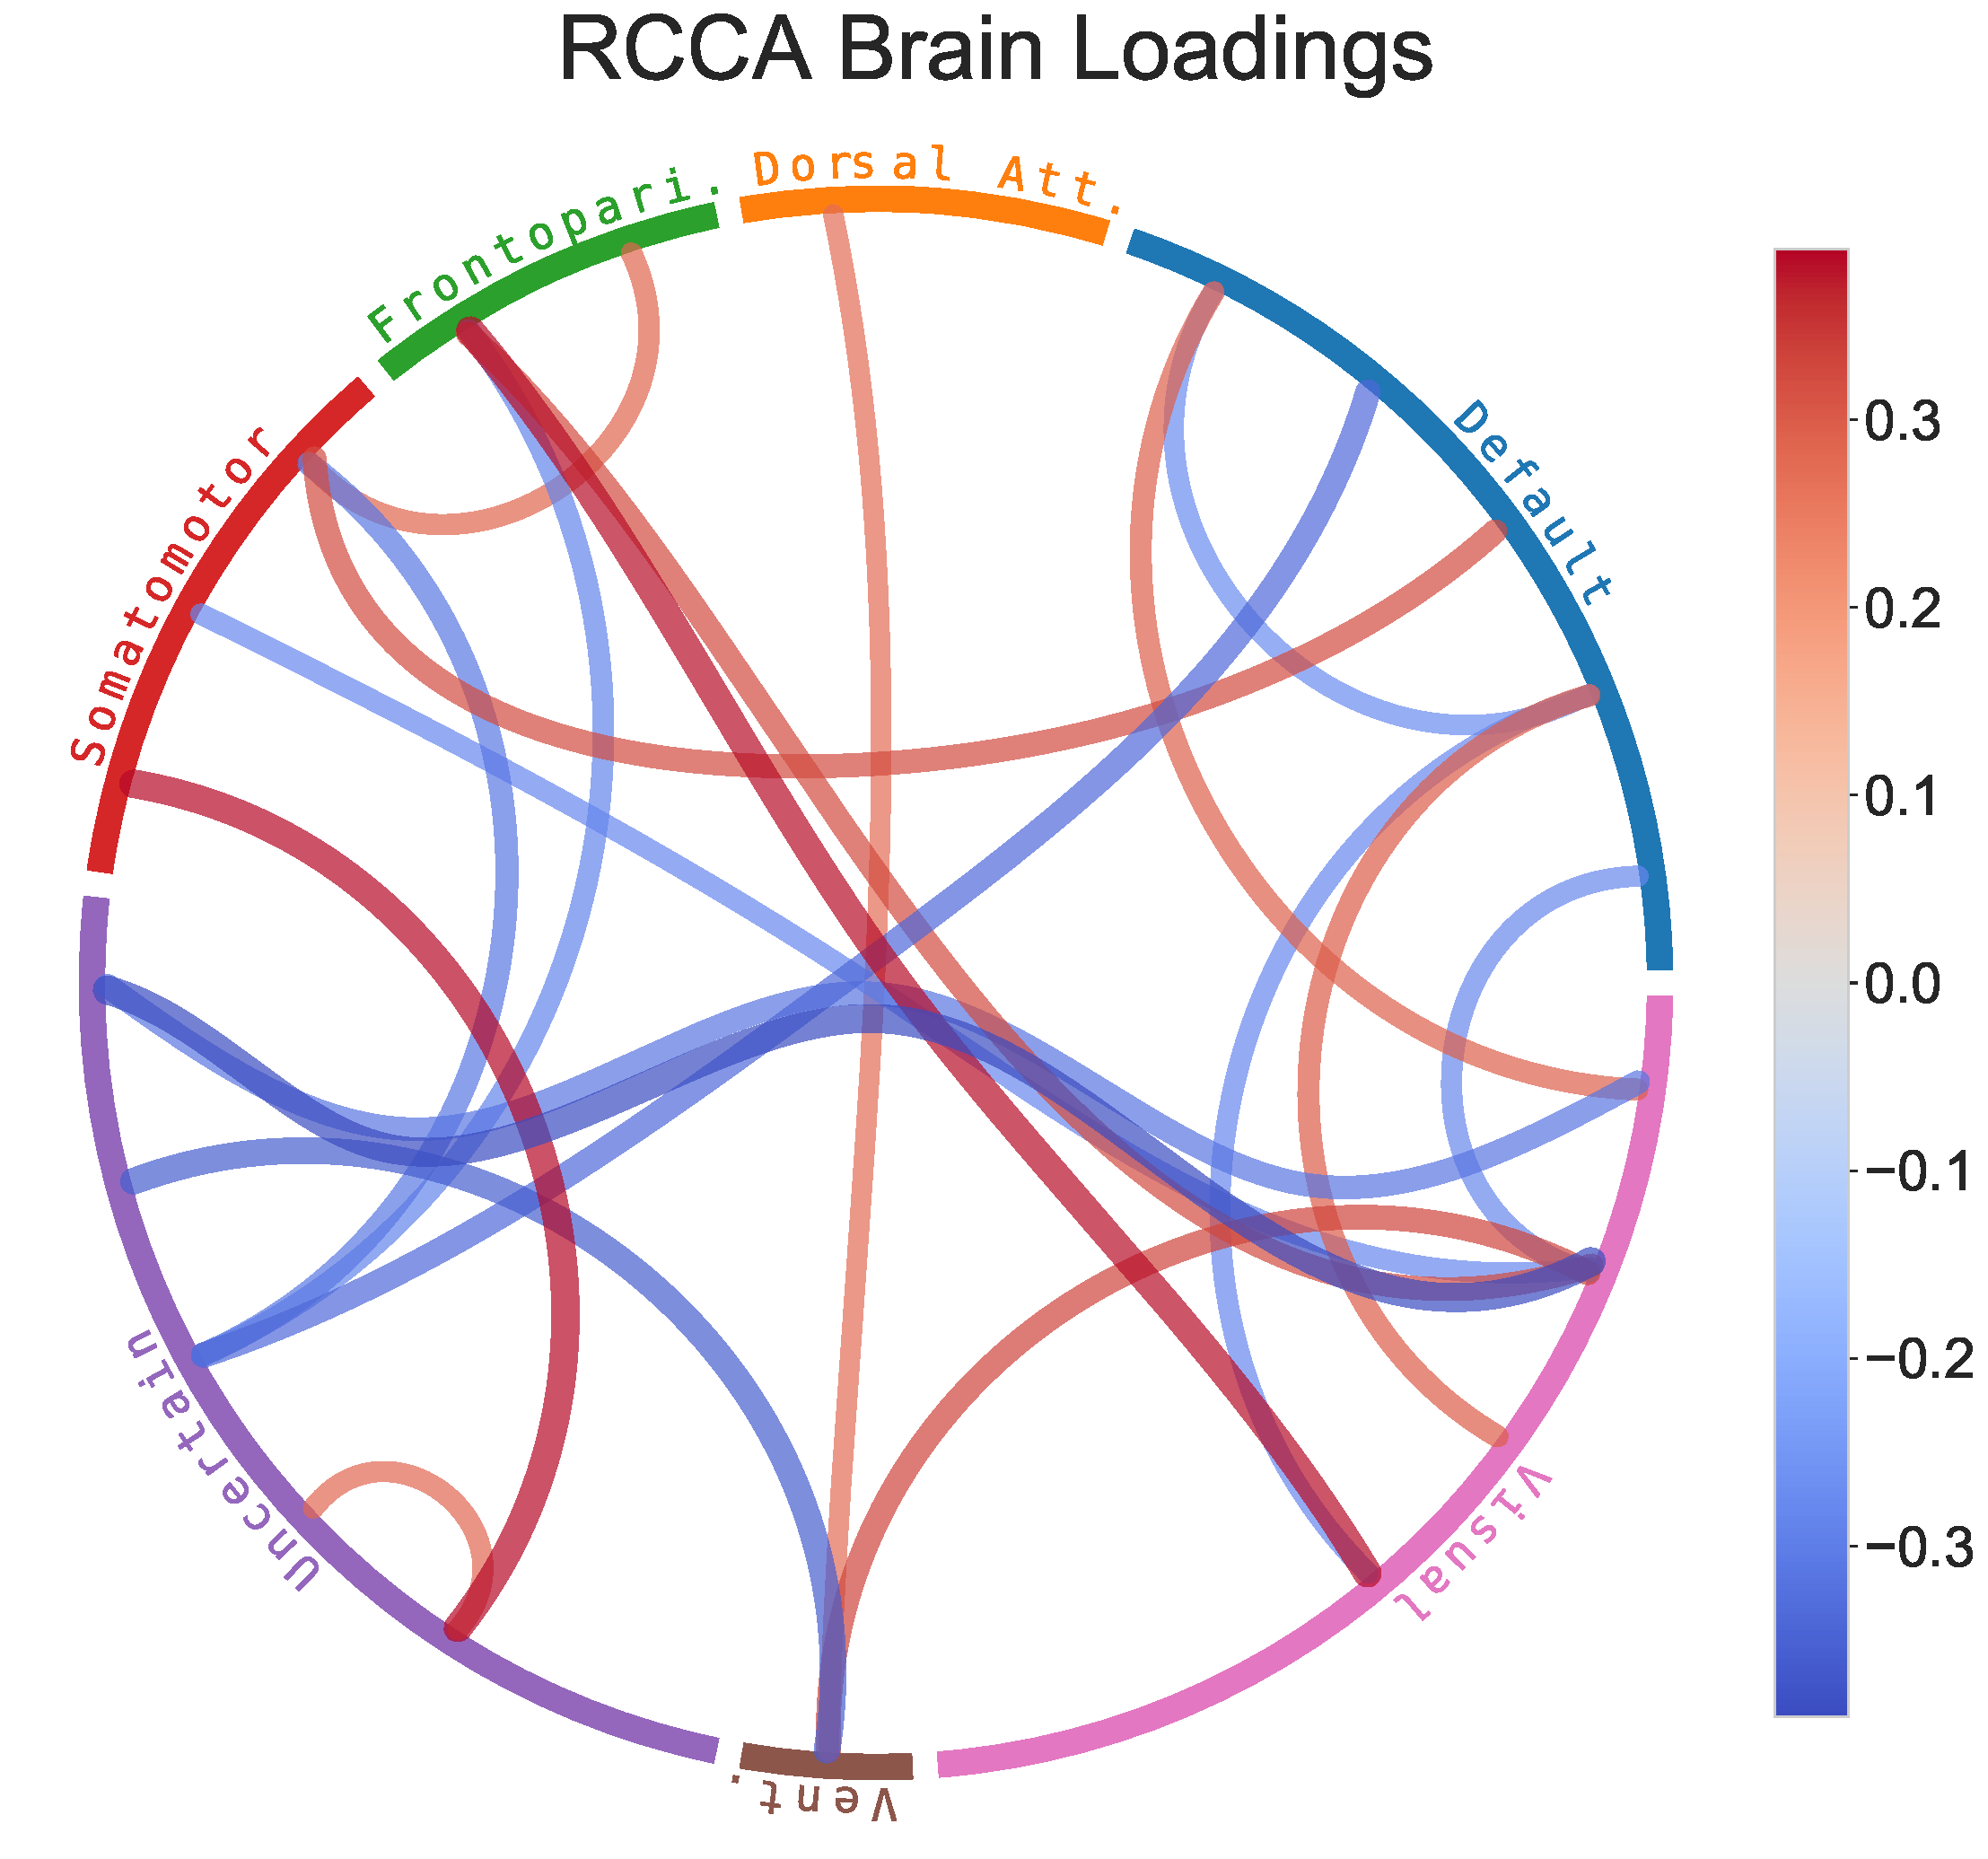
\includegraphics[width=0.49\linewidth]{figures/regularization/hcp/RCCA brain loadings}
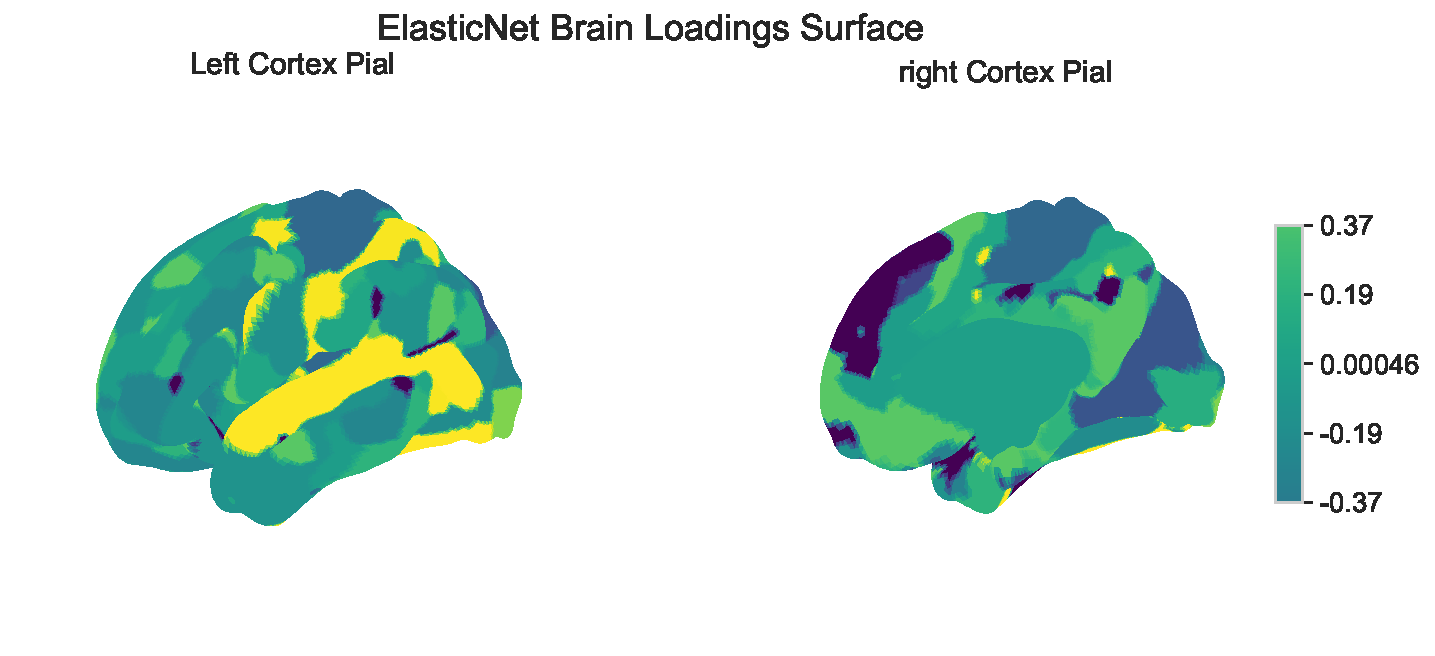
\includegraphics[width=0.49\linewidth]{figures/regularization/hcp/ElasticNet brain loadings}
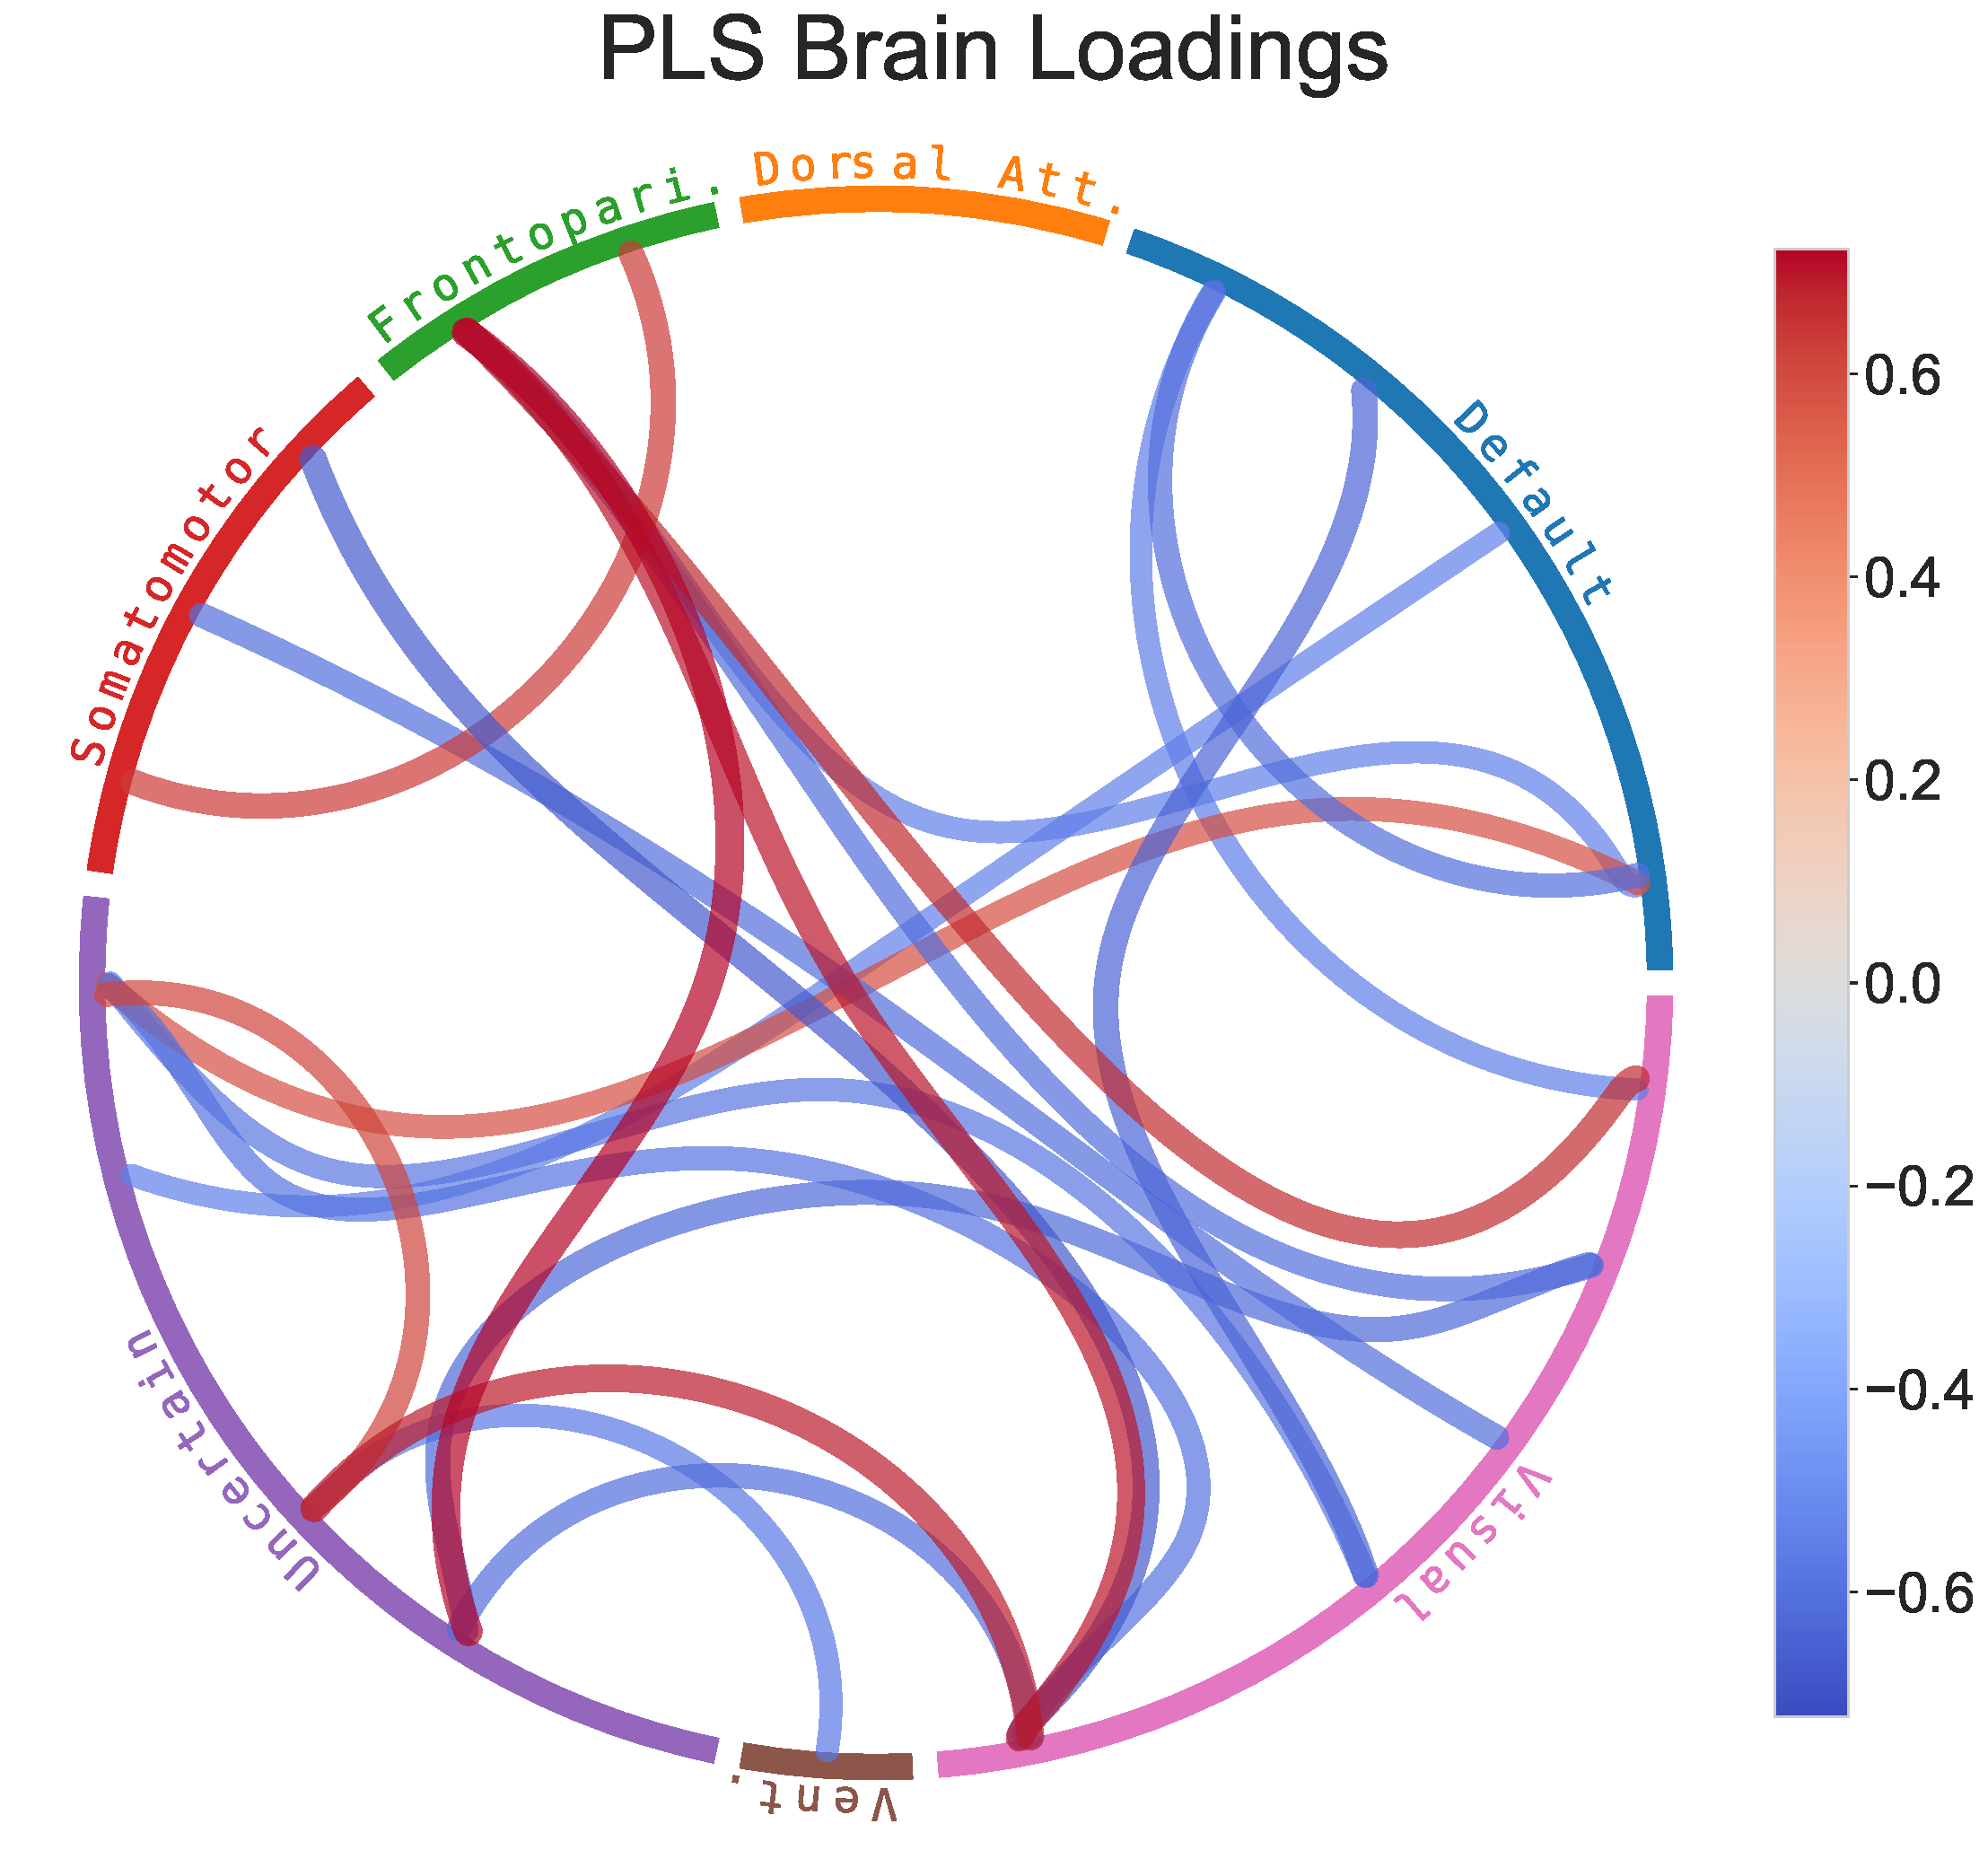
\includegraphics[width=0.49\linewidth]{figures/regularization/hcp/PLS brain loadings}
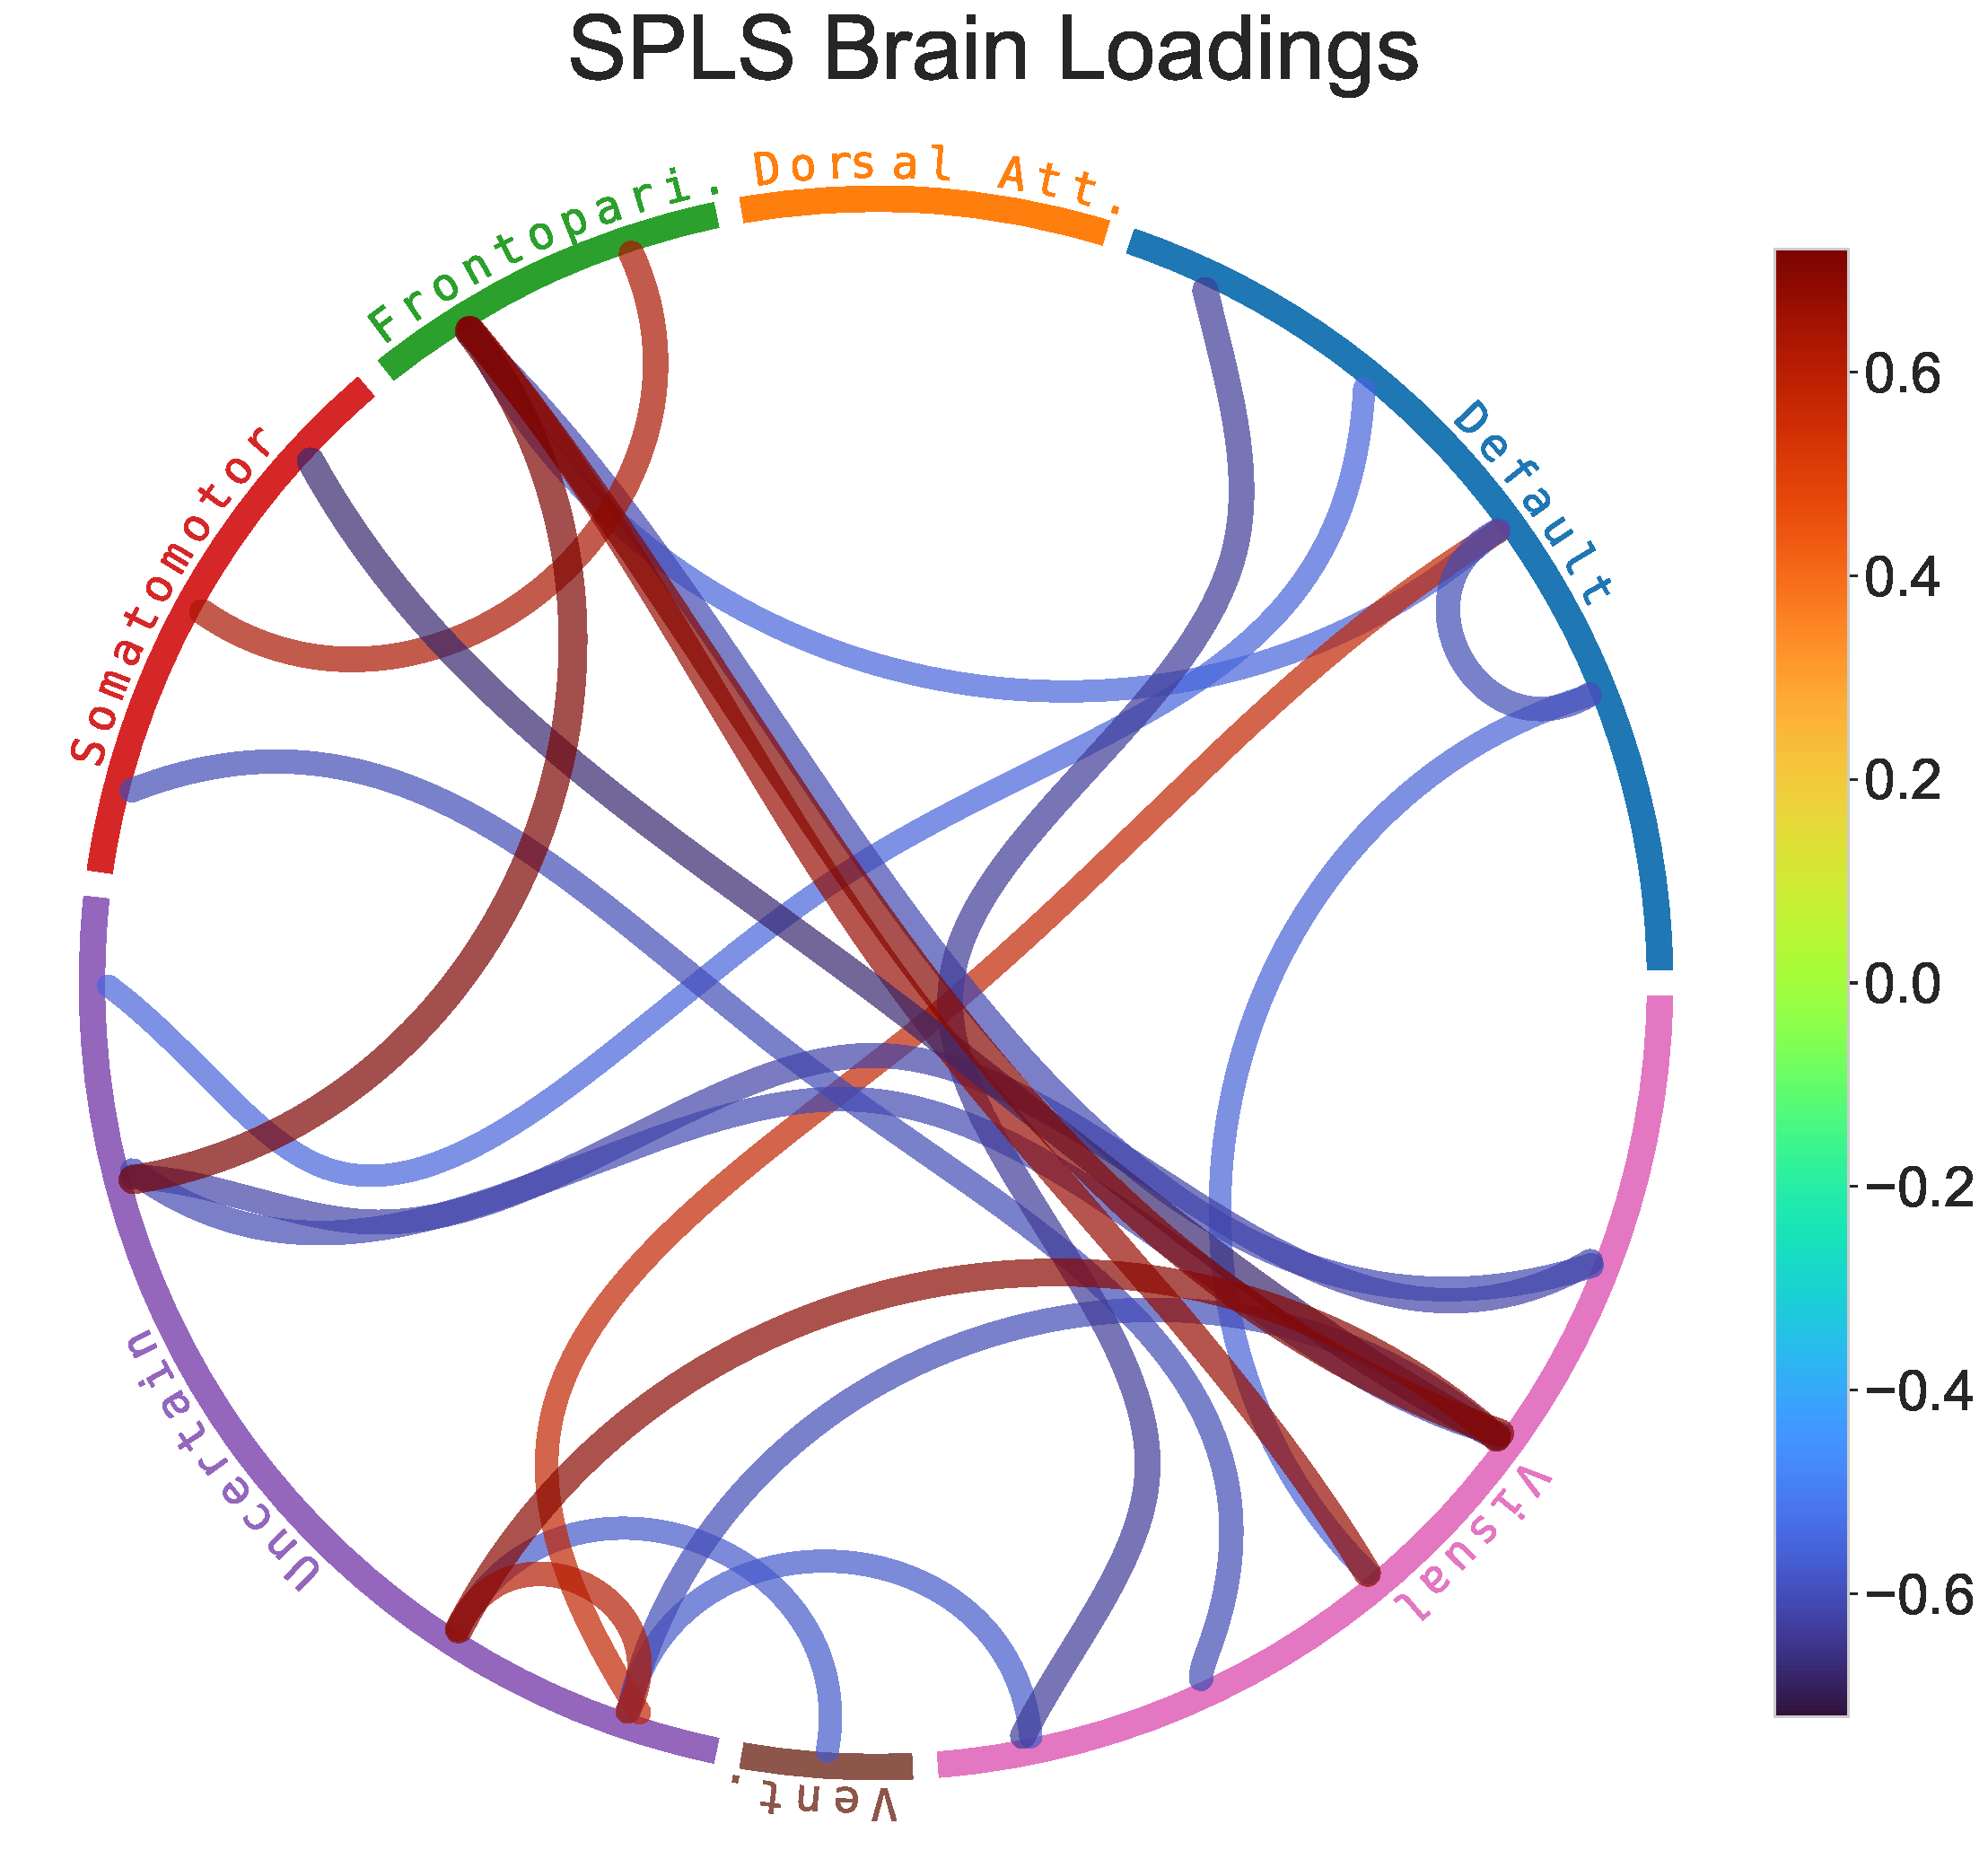
\includegraphics[width=0.49\linewidth]{figures/regularization/hcp/SPLS brain loadings}
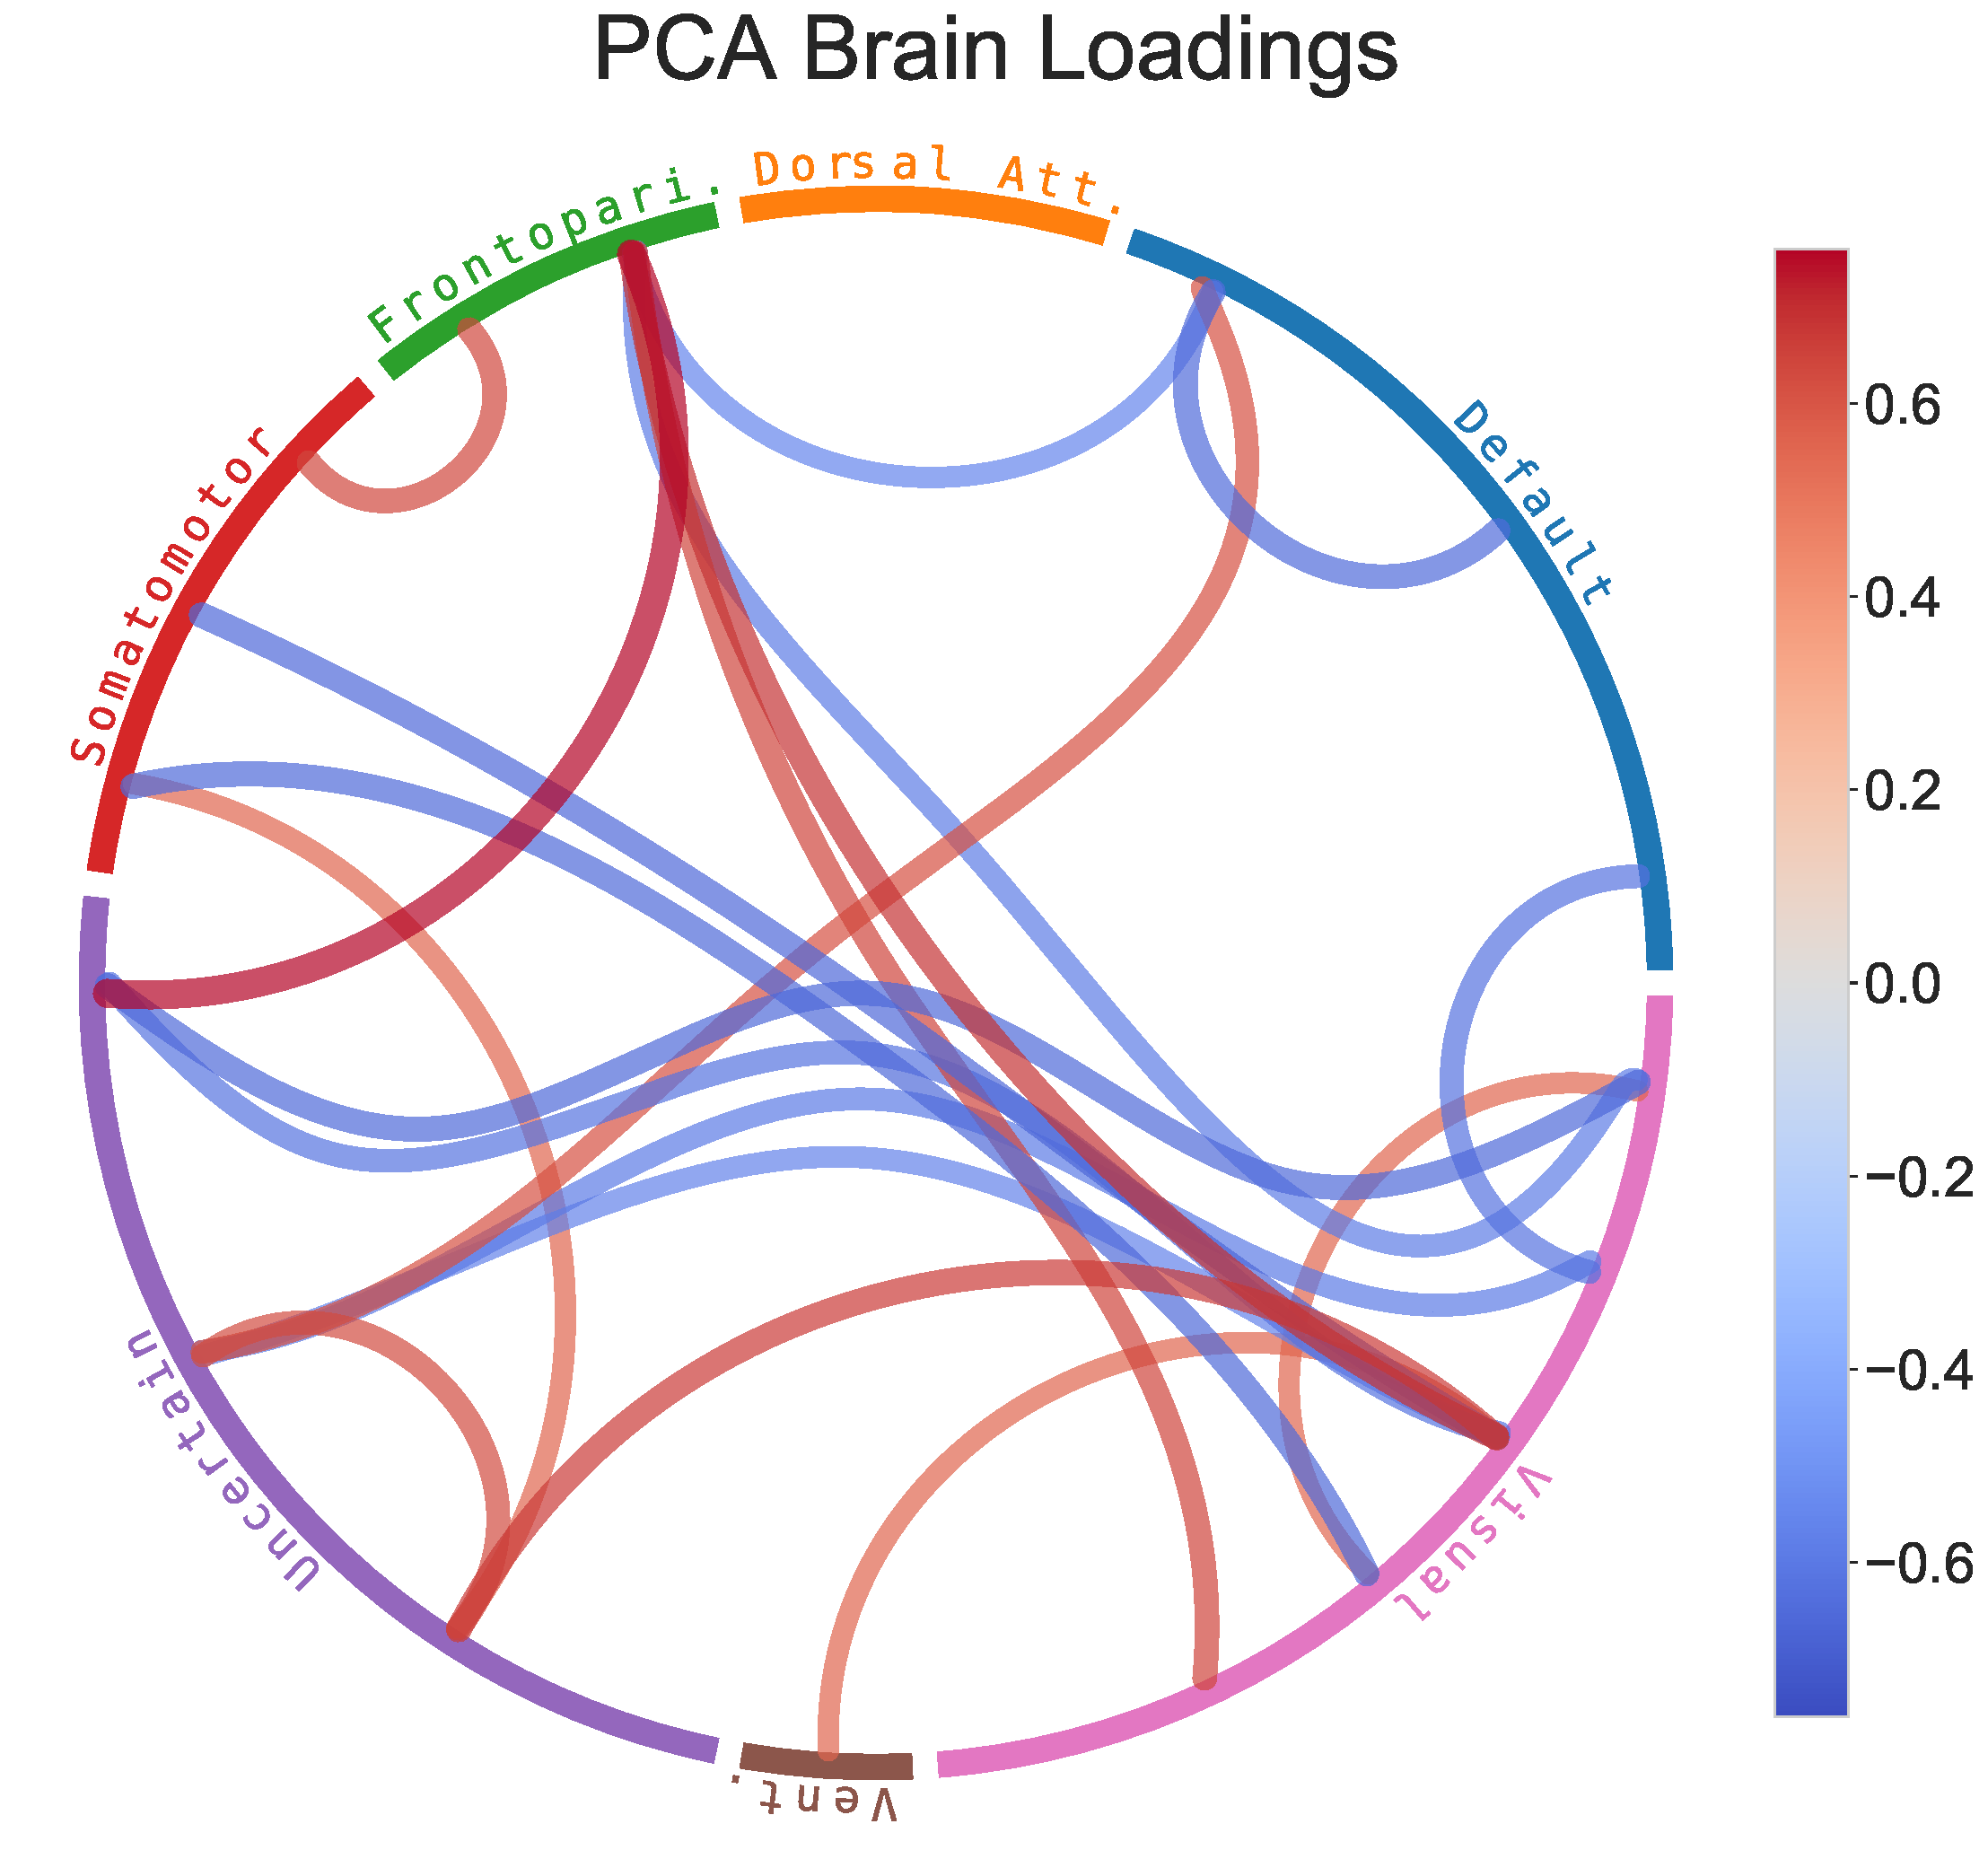
\includegraphics[width=0.49\linewidth]{figures/regularization/hcp/PCA brain loadings}
\caption{Chord diagrams of the top 8 positive and negative brain loadings for each model.}\label{fig:chord_loadings}
\end{figure}

\paragraph{Surface Map Parcellations}
The brain surface plots in Figure~\ref{fig:brain} represent maps of brain connection strength increases/decreases, which
were obtained by weighting each node’s parcel map with the GFA edge-strengths summed across the edges
connected to the node.
In Figure~\ref{fig:brain}, we show increases on the left and decreases on the right.

\textcolor{red} Need to find something biologically useful to say about these.
%
%\begin{figure}
%\centering
%\includegraphics[width=\linewidth]{figures/regularization/hcp/PCA brain loadings surface}
%\includegraphics[width=\linewidth]{figures/regularization/hcp/RCCA brain loadings surface}
%\includegraphics[width=\linewidth]{figures/regularization/hcp/ElasticNet brain loadings surface}
%\includegraphics[width=\linewidth]{figures/regularization/hcp/PLS brain loadings surface}
%\includegraphics[width=\linewidth]{figures/regularization/hcp/SPLS brain loadings surface}
%\caption{Map of CCA connection strength variations, with each node’s parcel map weighted by CCA edge-strength changes across edges involving that node.}\label{fig:brain}
%\end{figure}

\subsubsection{Sparsity of Weights}

Table \ref{tab:brain-behaviour-weights-hcp} shows the number of non-zero weights for each model.
We can see that tuned SPLS and Elastic Net do find sparse weights, but given the minimal difference in performance, it is not convincing evidence that this is a useful property.

\begin{table}[h]
\centering
\caption{Number of non-zero weights for each model.}
\begin{tabular}{|c|c|c|}
\hline
Model &  Brain Weights &  Behaviour Weights \\
\hline
PCA        &            300 &                145 \\
RCCA       &            300 &                145 \\
Elastic Net &            241 &                 96 \\
PLS        &            300 &                145 \\
SPLS       &            118 &                 56 \\
\hline
\end{tabular}\label{tab:brain-behaviour-weights-hcp}
\end{table}

\newpage
\subsection{Alzheimer's Disease Neuroimaging Initiative (ADNI) Data}\label{subsec:adni}

We now turn to the ADNI data where our analysis is similar but visualized differently.
This is because the ADNI data contains structural MRI data rather than functional MRI data.

\subsubsection{Out of Sample Correlation}

In this experiment, the Elastic Net model outperformed all other models in terms of out-of-sample correlation (Figure~\ref{fig:performance}).
The RCCA model also outperformed the PLS and SPLS models while SPLS outperformed PLS.
Suprisingly, PCA performed almost as well as PLS.

\begin{figure}
\centering
\includegraphics[width=0.5\linewidth]{figures/regularization/adni/holdout_correlations}
\caption{Out-of-sample canonical correlations for each model.}\label{fig:performance}
\end{figure}

\subsubsection{Behaviour Weights and Loadings}

As for the HCP data, Figure \ref{fig:adni-beh} plot the top 8 positive and negative non-imaging loadings and their associated weights for each model.
Some of the identified behavioural loadings including a number of orientation tests are similar across all of the models including even PCA.
This is indicative of the strong shared signal between the behavioural data and the brain structure data.
SPLS and Elastic Net both hone in on the orientation and recall tests in the weight space which appears also to translate to the loadings space.
The RCCA and Elastic Net models are suprisingly different in both the weight and loadings space, with the RCCA loading on a couple of attention and calculation tests in addition to the ubiquitous orientation and recall tests.

\begin{figure}
\centering
\includegraphics[width=0.8\linewidth]{figures/regularization/adni/PCA behaviour weights and loadings}
\includegraphics[width=0.8\linewidth]{figures/regularization/adni/RCCA behaviour weights and loadings}
\includegraphics[width=0.8\linewidth]{figures/regularization/adni/ElasticNet behaviour weights and loadings}
\includegraphics[width=0.8\linewidth]{figures/regularization/adni/PLS behaviour weights and loadings}
\includegraphics[width=0.8\linewidth]{figures/regularization/adni/SPLS behaviour weights and loadings}
\caption{Bar plots of the behaviour weights and loadings for each model.}\label{fig:adni-beh}
\end{figure}

\subsubsection{Brain Structure Weights and Loadings}

We plot the weights and loadings as a mosaic plot with 3 slices in each direction in Figure~\ref{fig:adni-brain}.
Previous work using SPLS with the ADNI dataset identified the same striking pattern of weights with the model strikingly selecting the hippocampal weights\cite{monteiro2016multiple}.
While the Elastic Net has a less visually appealing selection of weights, with a honeycomb pattern near the edges of the brain, the hippocampal region is more clearly loaded on in the loadings space (and likewise for RCCA).
It is noticeable that PCA, PLS and SPLS both weights in the same direction whereas RCCA and Elastic Net weight different regions with opposite signs.

\begin{figure}
\centering
\includegraphics[width=0.45\linewidth]{figures/regularization/adni/PCA brain loadings mosaic}
\includegraphics[width=0.45\linewidth]{figures/regularization/adni/PCA brain weights mosaic}
\includegraphics[width=0.45\linewidth]{figures/regularization/adni/RCCA brain loadings mosaic}
\includegraphics[width=0.45\linewidth]{figures/regularization/adni/RCCA brain weights mosaic}
\includegraphics[width=0.45\linewidth]{figures/regularization/adni/ElasticNet brain loadings mosaic}
\includegraphics[width=0.45\linewidth]{figures/regularization/adni/ElasticNet brain weights mosaic}
\includegraphics[width=0.45\linewidth]{figures/regularization/adni/PLS brain loadings mosaic}
\includegraphics[width=0.45\linewidth]{figures/regularization/adni/PLS brain weights mosaic}
\includegraphics[width=0.45\linewidth]{figures/regularization/adni/SPLS brain loadings mosaic}
\includegraphics[width=0.45\linewidth]{figures/regularization/adni/SPLS brain weights mosaic}
\caption{Statistical maps of brain structure loadings and weights for each model.}\label{fig:adni-brain}
\end{figure}

\subsubsection{Sparsity of Weights}

Table~\ref{tab:brain-behaviour-weights-adni} once again shows the number of non-zero weights for each model.
We can see that tuned SPLS and Elastic Net once again identify sparse weights.
In this case, the difference in performance is more convincing and suggests that this sparsity is less spuriously induced than for the HCP data.
This is supported by the fact that Elastic Net and SPLS models find a similar level of sparsity in the brain weights.
On the other hand SPLS finds a much sparser set of behavioural weights.

\begin{table}[h]
\centering
\caption{Number of non-zero weights for each model.}
\begin{tabular}{|c|c|c|}
\hline
Model &  Brain Weights &  Behaviour Weights \\
\hline
PCA        &         168130 &                 31 \\
RCCA       &         168130 &                 31 \\
Elastic Net &          59617 &                 17 \\
PLS        &         168130 &                 31 \\
SPLS       &          74995 &                 10 \\
\hline
\end{tabular}\label{tab:brain-behaviour-weights-adni}
\end{table}

\subsubsection{Identitiness of Covariance Matrices}
In this section, we consider the identitiness of the covariance matrices for the HCP and ADNI datasets.
Figure \ref{fig:covariance-eigenvalues-real} shows the eigenvalues of the covariance matrices for the HCP and ADNI datasets while Figure \ref{fig:covariance-matrices-real} shows the covariance matrices themselves (with the ADNI brain covariance matrix left out due to its size).
From Figure \ref{fig:covariance-eigenvalues-real}, we can see that the eigenvalues of the covariance matrices for the ADNI data are much closer to the ideal for identity covariance than for the HCP data.
\begin{figure}
\centering
\includegraphics[width=0.8\linewidth]{figures/regularization/covariance/hcp_adni_covariance_eigenvalues}
\caption{Eigenvalues of the covariance matrices for the HCP and ADNI datasets.}\label{fig:covariance-eigenvalues-real}
\end{figure}

From Figure \ref{fig:covariance-matrices-real}, we can see the block structure of the covariance matrices.

\begin{figure}
\centering
\begin{subfigure}{0.66\linewidth}
\centering
\includegraphics[width=\linewidth]{figures/regularization/covariance/HCP_covariance}
\caption{HCP}
\end{subfigure}
%
\begin{subfigure}{0.33\linewidth}
\centering
\includegraphics[width=\linewidth]{figures/regularization/covariance/ADNI_covariance}
\caption{ADNI}
\end{subfigure}
\caption{Covariance matrices for the HCP and ADNI datasets.}
\label{fig:covariance-matrices-real}
\end{figure}

This suggests that the only dataset and view where we can expect sparsity on the weights to imply sparsity on the loadings is the ADNI data and is consistent with the results we have seen in the previous section, that sparsity improves performance in the ADNI data but not in the HCP data.

\section{Discussion and Limitations}

In this section, we discuss the implications of our findings as well as the limitations of our study and the proposed FRALS method, some of which we address in later chapters of this thesis.

\subsection{Discussion}

\paragraph{Interpreting the Forward and Backward Models of CCA:} Consistent with \cite{haufe2014interpretation}, we have shown that assumptions imposed on the weights of a model do not in general transfer to the loadings.
This is because the weights and loadings are only equivalent when the covariance matrices are identity.
We have gone a step further than \cite{haufe2014interpretation} by showing that the identitiness of the covariance matrices is crucial for understanding how imposing sparsity on the weights imposes a prior belief in sparsity on the more biologically interesting loadings.

\paragraph{Sparsity on the weights does not imply sparsity on the loadings:}

On the other hand, our results raise the question of whether sparsity on the weights makes sense in the first place.
For latent variable models of brain-behaviour associations, we have argued that the loadings are the more biologically relevant quantity.
Since in practice, identity covariance is rarely a good assumption, the weights and loadings are not equivalent.
This means that sparsity on the weights does not imply sparsity on the loadings, and so we should not expect sparsity on the weights to lead to more interpretable loadings.
A practical step this implies is \textit{to ensure that the data covariances are at least close to identity before applying sparse CCA methods}.

\paragraph{Identitiness of real covariance matrices:} Between the HCP and ADNI datasets, only the ADNI data had eigenvalue spectra that were reasonably close to those of an identity matrix.
This suggests that the only dataset and view where we can expect sparsity on the weights to imply sparsity on the loadings is the ADNI data and is consistent with the results we have seen in the previous section, that sparsity improves performance in the ADNI data but not in the HCP data.
Furthermore, the loadings and weights are much more similar to each other in the ADNI data than in the HCP data, supporting the idea that the ADNI weights are themselves somewhat interpretable as estimates of the biologically relevant loadings.
Finally, in the well understood Alzheimer's disease data, we know that the identified weights (and loadings) are consistent with the known biology of the disease.

\paragraph{Sample versus Population Setting:} The results from the simulated data illustrate the disparities that can arise between population and sample settings.
Although PLS, RCCA, and CCA are equivalent under isotropic noise in a population framework, experiments showed that their performance can vary substantially in a sample setting.
In particular, this manifested as PLS underperforming RCCA and CCA under isotropic noise \textit{even though this is exactly the scenario where covariance identity holds and covariance thus equals correlation}.
This is because the sample covariance matrix is not the same as the population covariance matrix and PLS is sensitive to even small differences in the principal components of the sample covariance matrix.
Furthermore, in limited sample sizes, our estimations of the covariance matrices are not accurate, and so the identitiness of the covariance matrices is not guaranteed.
This generally resulted in poor estimation of loadings from model weights \textit{even when the weights themselves were estimated almost perfectly}.
Therefore, it's crucial for researchers to recognize these nuances and adopt appropriate measures when extrapolating results, especially in brain-behavior studies where typically only one sample is available and often limited in size.

\paragraph{Ridge CCA is typically much better than PLS across datasets:} Our results show that Ridge CCA is typically much better than PLS across datasets.
Much like regularised regression, it is unusual to need to use maximal ridge regularization even in high dimensions.
Our results in simulated data even cast doubt on the touted stability of PLS over CCA with respect to population CCA problem.
This means that while PLS might be more stable for a given dataset, it is not necessarily more stable across random samples from the same population.

\paragraph{Can We Construct a Regularization Functional that Imposes Sparsity on the Loadings?}
Finally, given our observations, a natural question to ask is whether we can construct a regularization functional that imposes sparsity on the loadings (instead of the weights).
The answer is yes, but it is not straightforward and in the small sample setting, it is not clear that it is a good idea.
The principle would be much the same as the Lasso, but we would need to use the sample covariance matrix to define the norm:

\begin{align}
    P(W)=\|W\|_1 \\
    P(L)=\|\hat{\Sigma}U\|_1
\end{align}

Which imposes an L1 penalty on the loadings via an L1 penalty on the weights multiplied by the sample covariance matrix.
We could in principle apply the soft-thresholding operator to the estimated loadings.
However we would need to be careful to ensure that the sample covariance matrix is invertible in order to get back to the weights.
This is of course not guaranteed in the small sample setting.

\subsection{Experiment Limitations}

\paragraph{Non-Gaussian Data:} The simulated data was generated from a Gaussian distribution.
This is a limitation of our study, and it would be interesting to see how the models perform on non-Gaussian data.
In particular, biomedical data typically contain categorical and even binary variables, and so it would be interesting to see how the models perform on such data.
We show an example of the Orientation category scores in the ADNI data in Figure~\ref{fig:adni-behavioural-data}.

\begin{figure}
\centering
\includegraphics[width=\linewidth]{figures/regularization/adni/Orientation}
\caption{Histogram of the Orientation test scores in the ADNI data.}\label{fig:adni-behavioural-data}
\end{figure}

\section{Conclusion}\label{sec:conclusion}

In this chapter, we have explored the performance of several CCA variants on simulated and real data.
We have shown that the choice of CCA variant can have a significant impact on the results.
We have also shown that the identitiness of the covariance matrices is crucial for understanding how imposing sparsity on the weights imposes a prior belief in sparsity on the more biologically interesting loadings.
We described a way to check the identitiness of the covariance matrices by looking at the eigenvalues of the covariance matrices and comparing to the ideal case.
We have also shown that FRALS can be a useful tool for brain-behaviour studies, but that it is computationally expensive.

In the next chapter, we address the scalability of CCA and its variants by introducing a novel algorithm based on gradient descent.

%
%\chapter{Gradient Descent: Accelerating CCA for Large Datasets}\label{ch:gradient_descent}
The content of this chapter is based on a preprint paper where I am first author.
I initiated the project based on heuristic arguments and contacted coauthors Ana Lawry Aguila (who provided and analysed the UK Biobank data) and Lennie Wells (who provided extensive mathematical proofs which are in the appendix of this PhD thesis for the interest of the reader).
Both of my coauthors helped me to revise the manuscript.
\minitoc

\section{Introduction}

Subspace learning techniques such as Canonical Correlation Analysis (CCA) have been essential tools in various scientific domains.
While these techniques are powerful, they face computational and scalability challenges, particularly for large datasets.
The focus of this chapter is to explore methods to effectively implement CCA using gradient descent and further scale it using stochastic gradient descent.
This chapter serves as a foundation for the application of proximal gradient descent in regularisation, which will be discussed in subsequent chapters.

\subsection{Problem Statement}

The existing methodologies for solving Canonical Correlation Analysis (CCA) face severe computational limitations, especially for large-scale datasets.
The challenges include high computational intensity and memory demands.

\subsection{Contributions}


\begin{itemize}
  \item Proposing an effective approach to solve CCA using gradient descent, laying the groundwork for future regularisation techniques using proximal gradient descent.
  \item Introducing a scalable methodology for applying CCA to large-scale medical datasets through stochastic gradient descent.
  \item Demonstrating the framework's effectiveness and scalability across diverse tasks and datasets.
  \item Providing a unique real-world application of stochastic PLS on an extremely high-dimensional biomedical dataset.
\end{itemize}

The subsequent sections will elaborate on these contributions, validating our approaches through various experimental setups and real-world applications.


\section{Background}
\subsection{Stochastic Approaches to CCA and PLS}

To the best of our knowledge, the state-of-the-art in Stochastic PLS and CCA are the subspace Generalized Hebbian Algorithm (\textbf{SGHA}) of \cite{chen2019constrained} and \textbf{$\gamma$-EigenGame} from \cite{gemp20,gemp2021}. Specifically, SGHA utilizes a Lagrange multiplier heuristic along with saddle-point analysis, albeit with limited convergence guarantees. EigenGame focuses on top-k subspace learning but introduces an adaptive whitening matrix in the stochastic setting with an additional hyperparameter.

\subsection{Reconstruction perspective on PCA and CCA}
The key idea behind this chapter relies on treating CCA as a low-rank approximation problem, rather than a constrained optimization problem or a generalized eigenvalue problem.

While this perspective is unusual in the context of CCA, it is well-known in the context of PCA. Indeed, the Eckart-Young-Mirsky theorem \cite{stewart_matrix_1990} states that the best rank-$k$ approximation to a matrix $M$ is given by the truncated SVD:

\begin{align}
    \argmin_{\substack{W \in \R^{d \times k} \\ W^T W = I}} \| M - W W^T M \|_F^2 = U_k \Sigma_k V_k^T
\end{align}

where $U_k \Sigma_k V_k^T$ is the truncated SVD of $M$. If we consider the case where $M=XX^T$, then this is precisely the PCA problem. 

This is a well-known result in matrix analysis, and it is often used to motivate PCA as a low-rank approximation problem. 
This reconstruction perspective is also the basis behind the Autoencoder, a popular deep learning architecture \cite{goodfellow2016deep}, which can be seen as a non-linear generalisation of PCA. 

In this chapter, we will show that a similar result holds for CCA and Generalized Eigenvalue Problems more generally, and that this can be used to motivate a new formulation of CCA as a low-rank approximation problem.


\section{Contributions}

In this section, we introduce a new class of algorithms based on matrix analysis results which allow us to efficiently solve a number of interesting problems including but not limited to CCA, PLS, DCCA, and SSL.

\subsection{GEP-GHA}
First, we present GEP-GH.

\begin{restatable}[Eckhart-Young inspired objective for GEPs]{proprep}{GHAcharac}
    \label{prop:GHA-charac}
    The top-$k$ subspace of the GEP $(A,B)$ can be characterised by maximising the following objective over $W \in \R^{d \times k}$:
    \begin{align}
        \mathcal{U}^\text{GEP-GHA}(W) \defeq \tr \left( 2\, W^T A W - \left(W^T A W\right) \left(W^T B W\right) \right)
    \end{align}
    Moreover, the maximum value is precisely $\sum_{j=1}^k \lambda_j^2$, where $(\lambda_j)$ are the generalised eigenvalues.
\end{restatable}

\subsection{Proof of Proposition \ref{prop:GHA-charac}}

\subsection{GEP-EY: an unconstrained objective for GEPs}

First, we present GEP-EY, a formulation of GEP problems by matrix analysis which permits efficient optimization by gradient descent.
This is summarised by proposition \ref{prop:EY-charac}, a consequence of applying the Eckhart-Young-Minsky inequality \cite{stewart_matrix_1990} to the eigen-decomposition of $B^\mhalf A B^\mhalf$. Detailed statements and proofs can be found in supplement \ref{supp:proofs}.

\begin{restatable}[Eckhart-Young inspired objective for GEPs]{proprep}{EYcharac}
    \label{prop:EY-charac}
    The top-$k$ subspace of the GEP $(A,B)$ can be characterised by maximising the following objective over $W \in \R^{d \times k}$:
    \begin{align}
        \mathcal{U}^\text{GEP-EY}(W) \defeq \tr \left( 2\, W^T A W - \left(W^T B W\right) \left(W^T B W\right) \right)
    \end{align}
    Moreover, the maximum value is precisely $\sum_{j=1}^k \lambda_j^2$, where $(\lambda_j)$ are the generalised eigenvalues.
\end{restatable}


In the following sections, we describe a number of algorithms for solving GEPs using proposition \ref{prop:EY-charac}.
These will be denoted with \textbf{EY} and \textbf{GHA}.

\subsection{Stochastic Optimization}

We next show how GEP-EY and CCA-SVD can be efficiently optimized using stochastic methods, which makes them suitable for large-scale and online settings.
Suppose we have an unbiased estimate $\hat{A}$ for $A$ and a pair of independent and unbiased estimates $(\hat{B},\hat{B}')$ of the matrix $B$ (for example obtained from a minibatch); then one can estimate the objective in proposition \ref{prop:constr-charac} by:
\begin{align}
    \hat{\mathcal{U}}^\text{GEP-EY}(W) \defeq \tr \left( 2\, W^T \hat{A} W - \left(W^T \hat{B} W\right) \left(W^T \hat{B}' W\right) \right)
\end{align}
which we can differentiate to give a gradient estimate:
\begin{align}\label{eq:GEP-EY-grad}
    \hat{\Delta}^{\text{GEP-EY}}(W)
    \defeq \nabla_W \hat{\mathcal{U}}^\text{GEP-EY}(W)
    % old = 4 \left\{ \hat{A} W - \hat{B} W \left(W^T \hat{B}' W \right) \right\}
    = 2 \left\{ 2 \hat{A} W - \hat{B} W \left(W^T \hat{B}' W \right) - \hat{B}' W \left(W^T \hat{B} W \right) \right\}
\end{align}

By the independence of $(\hat{B},\hat{B}')$ both of these estimates are unbiased.

The unbiased estimate immediately leads to Algorithm \ref{alg:Delta}.
The key advantage of this is that the computational complexity of the algorithm is only $\mathcal{O}(b d k)$; this is far less than the $\mathcal{O}(N d^2)$ complexity of any methods which evaluate the matrices $A,B$ on the full batch.

\textit{Why is the complexity so low?} Because $A,B$ are linear functions of covariance matrices, we can construct our unbiased estimates by plugging in sample covariances on a minibatch.
These estimates will then be low rank; indeed we can factorise these estimates in the form $\hat{M} \hat{M}^T$ where $\hat{M} \in \R^{d \times b}$. The dominant cost in evaluating $\mathcal{U}^\text{GEP-EY}$ is then just the matrix multiplications of the form $\hat{M}^T W$; see supplement \ref{supp:analyticsubspace} for full details.

\begin{algorithm}
    \caption{GEP-EY: A Stochastic Gradient Descent Algorithm for GEP subspace}
    \label{alg:Delta}
    \begin{algorithmic}
        \STATE {\bfseries Input:} data stream $Z_t$ consisting of B samples from $z_n$. Learning rate $(\eta_t)_t$. Number of time steps $T$. Number of eigenvectors to compute $k$.
        \STATE {\bfseries Initialise:} $(\hat{\mathbf {W}})_{i=1}^K$ with random uniform entries
        \FOR{$t=1$ {\bfseries to} $T$}
        \STATE Construct an independent unbiased estimate of $\hat{A}$ and two independent unbiased estimates of $\hat{B}$ from $Z_t$
        \STATE $\hat{\mathbf {W}} \leftarrow \hat{\mathbf {W}}+\eta_{t} \hat{\Delta}^{\text{GEP-EY}}$
        \COMMENT{As defined in (\ref{eq:GEP-EY-grad})}
        \ENDFOR
    \end{algorithmic}
\end{algorithm}

%%%%%%%%%%%%%%%%%%%%%%%%%%%%%%%%%%%%%%%%%%%%%%%%%%%%%%%%%%%%%%%%%%%%%%%%%%%%%%%%%%%%%%
%Stochastic CCA
%%%%%%%%%%%%%%%%%%%%%%%%%%%%%%%%%%%%%%%%%%%%%%%%%%%%%%%%%%%%%%%%%%%%%%%%%%%%%%%%%%%%%%
\section{Experiment 1: Application of CCA-EY to stochastic CCA}

\subsection{Experiment Design}

\subsubsection{Data}
\textbf{Mediamill}: The MediaMill dataset \cite{feng2004context} is a benchmark dataset for multilabel classification
. It consists
of 1200 video clips from the TRECVID 2003 conference, each annotated with 101 labels. The original goal of the dataset was to predict the labels of the videos from the visual and audio features. It has since become a benchmark dataset for CCA and other multiview learning methods. We use the same features as \cite{gemp2022generalized} which are 128-dimensional bag-of-visual-words features and 13-dimensional bag-of-audio-words features. We split the data into 80\% train and 20\% test and use cross-validation within the training data in order to tune hyperparameters.

\textbf{Split CIFAR}: The CIFAR-10 dataset \cite{krizhevsky2009learning} consists of 60,000 32x32 colour images in 10
classes, with 6000 images per class. There are 50,000 training images and 10,000 test images. We split the images into two halves.

In this section, we compare GEP-GD and CCA-SVD to $\gamma$-EigenGame \cite{gemp2022generalized} and SGHA \cite{chen2019constrained} for approximating CCA in the stochastic setting. Replicating the experiment in \cite{meng2021online, gemp2022generalized}, we optimize for the top-4 CCA subspace for the MediaMill and Split CIFAR (left and right halves of CIFAR-10 images) datasets. We use a minibatch size 100 and train for one epoch across 5 random seeds (with 1 standard deviation error bars in the plots). We use the Scipy \cite{virtanen2020scipy} package to solve the full batch GEPs as a ground truth value and use the proportion of correlation captured (PCC) captured by the learnt subspace as compared to this ground truth (defined in supplement \ref{supp:experimental details}). Unlike \cite{gemp2022generalized}, we do not perform PCA on the data before applying the CCA methods but instead, for the MNIST data, we add gaussian noise to avoid zero variance subspaces in $X$ and $Y$. This makes our task more challenging, as performing PCA simplifies the problem by substituting $B$ for the identity matrix $I$. This explains the decrease in performance of $\gamma$-EigenGame as compared to their original work.


\subsection{Results}

Figure \ref{fig:ccaiter} shows that both of our methods outperform SGHA and $\gamma$-EigenGame on both datasets in terms of speed of convergence and achieve near-optimal performance in terms of PCC after just one epoch. All of the algorithms share the same complexity per iteration so that these results are also representative in terms of runtime. This demonstrates the effectiveness and superiority of our method for solving CCA in the stochastic setting.

\begin{figure}%[H]
    \centering
    \begin{subfigure}[b]{0.49\textwidth}
        \centering
        \includegraphics[width=\textwidth]{figures/gradient_descent/CCA/mediamill_100_pcc_lr_tuned.png}
        \label{fig:ccamediamill}
    \end{subfigure}
    \hfill
    \begin{subfigure}[b]{0.49\textwidth}
        \centering
        \includegraphics[width=\textwidth]{figures/gradient_descent/CCA/cifar_100_pcc_lr_tuned.png}
        \label{fig:ccacifar}
    \end{subfigure}
    \caption{PCC with respect to Scipy ground truth by GEP-EY and CCA-SVD vs prior work for (a) MediaMill and (b) Split CIFAR data. The maximum value is 1.0 and shading represents $\pm$ 1 standard deviation.}
    \label{fig:ccaiter}
    \label{fig: stochasticcca}
\end{figure}

\subsubsection{Stochastic CCA Minibatch Size}
In this section, we take a closer look at how minibatch sizes impact the performance of our method in the stochastic CCA setting. We maintain a constraint of single epoch training. This means that when we use smaller minibatches, the number of training steps increases correspondingly.

Our experiments, as displayed in Figure \ref{fig:minibatch size ablation}, show that our method performs well across a range of minibatch sizes. Notably, it achieves high performance even when the minibatch size is nearly equivalent to the number of components.

This indicates that our method can learn effectively from a limited number of samples. It suggests the possibility of applying our method to analyse large datasets on devices with restricted memory, by processing small minibatches of data sequentially. This robustness to minibatch size could potentially make our method a viable solution for large-scale data analysis where computational resources are limited.

\begin{figure}[h]
    \centering
    \begin{subfigure}[b]{0.49\textwidth}
        \centering
        \includegraphics[width=\textwidth]{figures/gradient_descent/CCA/cifar_minibatch_size_ablation.png}
        \caption{}
        \label{fig:cifar_minibatch_ablation}
    \end{subfigure}
    \begin{subfigure}[b]{0.49\textwidth}
        \centering
        \includegraphics[width=\textwidth]{figures/gradient_descent/CCA/mediamill_minibatch_size_ablation.png}
        \caption{}
        \label{fig:mediamill_minibatch_ablation}
    \end{subfigure}
    \caption{Ablation study on minibatch size for stochastic CCA for (a) cifar and (b) mediamill datasets for minibatch sizes 100, 20, and 5}
    \label{fig:minibatch size ablation}
\end{figure}

\subsection{Discussion}



%Stochastic PLS UKBB
%%%%%%%%%%%%%%%%%%%%%%%%%%%%%%%%%%%%%%%%%%%%%%%%%%%%%%%%%%%%%%%%%%%%%%%%%%%%%%%%%%%%%%
\section{Experiment 2: Application of PLS-EY to PLS on large scale biomedical data}

\subsection{Experiment Design}

\subsection{Data}
\textbf{The UK Biobank}: is arguably the largest scale biomedical database in the world with around half a
million
total participants. The goal is to have imaging data for the brain, heart, and body for 100,000 participants. The UK Biobank combines these images with genetics, biomarkers, electronic health record, and online questionnaires making it a rich dataset for broad studies of health.

For the GEP-EY PLS analysis on biomedical data, we used 33,333 subjects from the UK Biobank \cite{sudlow2015uk}. We used pre-processed (using FreeSurfer \cite{Fischl2012}) grey-matter volumes for 66 cortical (Desikan-Killiany atlas) and 16 subcortical brain regions and 582,565 autosomal genetic variants. The affects of age, age squared, intracranial volume, sex, and the first 20 genetic principal components for population structure were removed from the brain features using linear regression to account for any confounding effects. Each brain ROI was normalised by removing the mean and dividing the standard deviation. We processed the genetics data using PLINK \cite{Purcell2007} keeping genetic variants with a minor allele frequency of at least 1\%  and a maximum missingness rate of 2\%. We used mean imputation to fill in missing values and centered each variant.

To generate measures of genetic disease risk, we calculated polygenic risk scores using PRSice \cite{PRSice2014}. We calculated scores, with a p-value threshold of 0.05, using GWAS summary statistics for the following diseases; Alzheimer's \cite{Lambert2013}, Schizophrenia \cite{Trubetskoy2022}, Bipolar \cite{Mullins2021}, ADHD \cite{Demontis2023}, ALS \cite{Van_Rheenen2021}, Parkinson's \cite{Nalls2019}, and Epilepsy \cite{International_League_Against_Epilepsy_Consortium_on_Complex_Epilepsies2018}, using the referenced GWAS studies.

We demonstrate the power of GEP-EY for large-scale subspace learning by solving PLS on imaging genetics data from the UK Biobank \cite{sudlow2015uk}, a biomedical database.
This can reveal novel phenotypes of interest and uncover genetic mechanisms of disease and brain morphometry.
Previous imaging genetics analyses using PLS and CCA were limited to small-scale datasets \cite{Lorenzi2018,Taquet2021,Lefloch2012}, which are prone to overfitting and instability.
Full batch approaches are infeasible for this data due to the high computational cost.
The only other large-scale PLS analysis on the UK Biobank used a federated approach with local batch PLS-SVD \cite{lorenzi2016}, which approximates the global solution.
We present the first stochastic PLS analysis on large-scale biomedical data.

We ran GEP-EY with minibatch size 500 on brain imaging (82 regional volumes) and genetics (582,565 variants) data for 33,333 subjects; a massive amount of data that challenges existing methods.
See supplement (Section \ref{sec:ukbb_preprocessing}) for data pre-processing details.
We see strong validation correlation between all 10 corresponding pairs of vectors in the PLS subspace and weak cross correlation, indicating that our model learnt a coherent and orthogonal subspace of covariation (Figure \ref{fig:UKBB_corr}), a remarkable feat for such high-dimensional data.
We found that the PLS brain subspace was associated with genetic risk measures for several disorders (Figure \ref{fig:genetic_risk}), suggesting that the PLS subspace encodes relevant information for genetic disease risk, a significant finding for biomedical research.


% First Figure
\begin{figure}
    \centering
    \includegraphics[width=0.5\textwidth,trim={0.8cm 0cm 0.3cm 0cm}]{figures/gradient_descent/UKBB/cross_corr}
    \caption{Correlations between PLS components for UK Biobank. This figure shows strong validation correlation between all 10 corresponding pairs of vectors in the PLS subspace and weak cross correlation, demonstrating that our model has learned a coherent and orthogonal subspace of covariation.}
    \label{fig:UKBB_corr}
\end{figure}

% Second Figure
\begin{figure}
    \centering
    \includegraphics[width=0.7\textwidth,trim={0.5cm 0cm 0.7cm 0cm}]{figures/gradient_descent/UKBB/prs_correlations}
    \caption{Correlations between PLS brain components and genetic risk scores for several disorders. AD=Alzheimer's disease, SCZ=Schizophrenia, BP=Bipolar, ADHD=Attention deficit hyperactivity disorder, ALS=Amyotrophic lateral sclerosis, PD=Parkinson's disease, EPI=Epilepsy. The p-value significance levels are indicated as $\text{ns}: 0.05< p <= 1, \ast: 0.01< p <=0.05, \ast\ast: 0.001< p <= 0.01, \ast\ast\ast: 0.0001< p <= 0.001$. This suggests that the PLS subspace encodes relevant information for assessing genetic disease risk, an important contribution to biomedical research.}
    \label{fig:genetic_risk}
\end{figure}


\subsection{Discussion and Conclusion}

\section{Conclusion}

We presented a new unconstrained objective to characterise GEPs; this immediately gave efficient algorithms to solve many subspace learning methods in the stochastic setting with SGD.
Crucially, the gradient estimates are unbiased and cheap to compute.
Moreover, the only hyperparameter is the choice of optimiser.
We will later show how this work can be adapted and applied to optimise regularised GEPs and, in particular, CCA.

\appendix

\section{Appendix}
%
%\chapter{Proximal Gradient Descent: A Flexible, Scalable Approach to Regularised CCA}
\label{ch:proximal-gradient-descent}
\minitoc

% And this gives us the generalized eigenvalue problem~\citep{rosipal2005overview}:

% \begin{align}
%     \begin{pmatrix}
%         0 & \hat{\Sigma_{12}} \\
%         \hat{\Sigma_{21}} & 0 
%     \end{pmatrix} \begin{pmatrix}
%         u^{(1)} \\
%         u^{(2)}
%     \end{pmatrix}= \begin{pmatrix}
%         (1-c_1)\hat{\Sigma_{11}} + c_1I & 0 \\
%         0 & (1-c_2)\hat{\Sigma_{22}} + c_2I
%     \end{pmatrix}\begin{pmatrix}
%         u^{(1)} \\
%         u^{(2)}
%     \end{pmatrix}
% \end{align}

% The main difference between this eigenvalue problem and the CCA eigenvalue problem is the substitution of the matrices \(\Sigma_{11}\) and \(\Sigma_{22}\) for the matrices \( ((1-c_1) \Sigma_{11} + c_1 I) \) and \( ((1-c_2) \Sigma_{22} + c_2 I) \).
% We can therefore see that this regularisation is equivalent to adding a constant `ridge' to the diagonal of the covariance matrix \(X\spstop{i} X\sps{i}\).

\section{Introduction}

High-dimensional data are now more prevalent than ever, presenting both opportunities and challenges.
Canonical Correlation Analysis (CCA), despite its utility, struggles with high-dimensional datasets, resulting in problems like overfitting and computational inefficiency.
The CCA-EY formulation, introduced in the previous chapter, partially addresses these issues but leaves room for improvement, particularly for large-scale neuroimaging datasets.
This chapter aims to bridge this gap by incorporating regularization techniques via proximal gradient descent.

\section{Problem Statement}

The application of CCA in high-dimensional settings, such as neuroimaging data containing tens of thousands of subjects and features, often leads to overfitting.
While CCA-EY has mitigated some challenges, there remains a critical need for a methodology that can handle large-scale, high-dimensional data without sacrificing interpretability or computational efficiency.

\section{Contributions}

Our contributions in this chapter are as follows:

\begin{itemize}
    \item We integrate regularization into the CCA-EY framework to explicitly tackle the high-dimensionality problem. See \textit{Section X} for technical details.
    \item We employ proximal gradient descent to optimize the regularized objective function, creating a method that is both scalable and interpretable.
    \item A comparative analysis against existing techniques validates the effectiveness of our approach.
    \item A case study demonstrates the real-world applicability of the proposed method. Refer to \textit{Section X} for an in-depth look at the implementation and results.
\end{itemize}

In summary, this chapter introduces a robust, scalable, and interpretable extension to the CCA-EY framework to better analyze high-dimensional, multimodal data.

\section{Background}

\subsection{Proximal Gradient Descent}

Proximal Gradient Descent is an optimization algorithm commonly used for solving non-smooth convex optimization problems.
The general objective function can be expressed as \( f(x) + g(x) \), where \( f(x) \) is a differentiable convex function and \( g(x) \) is a non-differentiable convex function.
The algorithm iteratively updates \( x \) using the following equation:

\[
x^{(k+1)} = \text{prox}_{\alpha g} \left( x^{(k)} - \alpha \nabla f(x^{(k)}) \right)
\]

Here, \( \alpha \) is the step size, \( \nabla f(x^{(k)}) \) is the gradient of \( f \) at \( x^{(k)} \), and \( \text{prox}_{\alpha g}(v) \) is the proximal operator defined as:

\[
\text{prox}_{\alpha g}(v) = \arg\min_{x} \left( g(x) + \frac{1}{2\alpha} \| x - v \|^2 \right)
\]

By combining the gradients of the smooth part \( f(x) \) and the proximal operator of the non-smooth part \( g(x) \), proximal gradient descent is capable of solving problems that are otherwise intractable using basic gradient descent.

\subsection{Total Variation Regularization}

Total Variation (TV) Regularization is a regularization technique often used for signal denoising and image reconstruction. The TV norm of a signal \( x \in \mathbb{R}^n \) is given by:

\[
\| x \|_{TV} = \sum_{i=1}^{n-1} |x_{i+1} - x_i|
\]

In a 2D image, the TV norm extends to:

\[
\| x \|_{TV} = \sum_{i,j} \sqrt{(x_{i+1,j} - x_{i,j})^2 + (x_{i,j+1} - x_{i,j})^2}
\]

When incorporated as a regularizer \( R(x) \) in an optimization problem, it typically takes the form:

\[
\min_{x} \; f(x) + \lambda \| x \|_{TV}
\]

where \( \lambda \) is the regularization parameter that controls the trade-off between the data fidelity term \( f(x) \) and the regularizer \( \| x \|_{TV} \).

By leveraging TV regularization, one can impose piecewise-smoothness on the solution, making it particularly useful for preserving edges in images or abrupt changes in signals.

\subsection{GraphNet Regularization in Neuroimaging}

While Elastic-Net regression offers a balance between ridge and lasso penalties, it lacks the ability to explicitly model spatial and temporal structures inherent in neuroimaging data.
This is where GraphNet—an extension of the Elastic-Net—comes into play.

\textbf{GraphNet Formulation}: GraphNet incorporates an additional penalty term linked with a graph \(G\), which could be a Laplacian matrix \(L = D - A\).
The graph Laplacian captures our intuition that voxels which are neighbors in both space and time should have similar activation levels:

\[
\text{GraphNet Penalty} = \lambda_{1} \lVert \beta \rVert_{1} + \lambda_{2} \beta^T G \beta
\]

Here, \(\beta(x, y, z, t)\) represents coefficients across the 4D spatio-temporal brain volume, and \(\lambda_{1}\) and \(\lambda_{2}\) are regularization parameters. When \(G = L\), the penalty term morphs into:

\[
\sum_{(i, j) \in \epsilon_{G}} (\beta_{i} - \beta_{j})^{2}
\]

\textbf{Preserving Smoothness in the Brain}: One of the core advantages of using GraphNet in neuroimaging is its ability to maintain smoothness across the brain map.
Unlike methods like Total Variation, which may create piecewise constant structures, GraphNet aims to create a spatially smooth map.
This is aligned with the nature of fMRI data, where spatial smoothness is often expected.

\textbf{Algorithmic Simplicity and Efficiency}: The quadratic nature of the GraphNet penalty avoids the algorithmic complexities often seen in non-smooth penalties.
This is particularly important in high-dimensional neuroimaging data where computational efficiency is crucial.

\textbf{Flexibility in Model Constraints}: GraphNet allows for user-specified constraints to be easily integrated into the model, making it flexible for a variety of neuroimaging applications.

In summary, GraphNet offers a regularization technique that is not only sparse but also structured in a way that respects the spatial and temporal smoothness inherent in brain data.
This makes it a compelling choice for neuroimaging applications where a smooth representation of the brain is desired.


\section{Contributions}
\subsection{Proximal CCA-EY}
We introduce a formulation called Proximal CCA-EY that extends the Generalized Eigenvalue Problem (GEP) formulation for CCA. In this extended formulation, \( W = (W_1, W_2) \), with each set of weights potentially subject to a different regularization term.
By adding regularization terms to the objective function, we can solve this regularized GEP using proximal gradient descent algorithms.
This approach permits the use of a variety of regularization functions, which we demonstrate can be efficiently computed.
Algorithm details are similar to those shown in Algorithm 1 in the previous section, with additional steps to include the proximal operators corresponding to the chosen regularization terms for each \( W_i \).

\begin{equation}
\label{eq:proximal-CCA-EY}
    \mathcal{U}^{\text{Proximal CCA-EY}}(W_1, W_2) = \mathcal{L}^{\text{EY}}(W_1, W_2) + \lambda_1 \mathcal{R}_1(W_1) + \lambda_2 \mathcal{R}_2(W_2)
\end{equation}

Here, \( \lambda_1 \) and \( \lambda_2 \) are hyperparameters that control the strength of the regularization terms, and \( \mathcal{R}_1(W_1) \) and \( \mathcal{R}_2(W_2) \) can be any functions for which proximal operators can be efficiently computed.
Specific implementations for \( L_1 \) and Total Variation regularizations are provided for both \( W_1 \) and \( W_2 \).

The proximal gradient descent update for this problem is then given by:

\begin{equation}
\label{eq:proximal-update}
    W_1^{(t+1)} = \text{prox}_{\alpha \lambda_1 \mathcal{R}_1}\left( W_1^{(t)} - \alpha \nabla_{W_1} \mathcal{L}^{\text{EY}}(W_1^{(t)}, W_2^{(t)}) \right)
\end{equation}

\begin{equation}
\label{eq:proximal-update-W2}
    W_2^{(t+1)} = \text{prox}_{\alpha \lambda_2 \mathcal{R}_2}\left( W_2^{(t)} - \alpha \nabla_{W_2} \mathcal{L}^{\text{EY}}(W_1^{(t)}, W_2^{(t)}) \right)
\end{equation}

Where \( \alpha \) is the learning rate, and \( \text{prox}_{\alpha \lambda_i \mathcal{R}_i} \) is the proximal operator for \( \alpha \lambda_i \mathcal{R}_i \).

\subsubsection{L1 Regularization}
For \( L_1 \) regularization, \( \mathcal{R}_i(W_i) = \| W_i \|_1 \), and the proximal operator becomes a simple soft-thresholding operation.

\subsubsection{Total Variation Regularization}
For Total Variation regularization, \( \mathcal{R}_i(W_i) = \text{TV}(W_i) \), where TV stands for the Total Variation.
The corresponding proximal operator can be efficiently computed using existing methods.

\subsection{ProxTorch}

The field of constrained and regularized optimization has a range of software tools designed for specialized tasks \citep{Moolekamp, ParsimonY}. Some of these tools, such as PyProximal \citep{pyproximal}, are restricted to numpy-based computational environments. Meanwhile, PyTorch \citep{paszke2019pytorch}, a deep learning framework with dynamic computation graph and GPU support, did not offer native integration for proximal operators. 

\texttt{ProxTorch} was developed to provide a comprehensive library of proximal operators that are compatible with PyTorch tensors. This compatibility allows for more streamlined development and optimization processes for models that incorporate proximal operators, all within the PyTorch framework.

\subsubsection{GPU Acceleration}

The performance of \texttt{ProxTorch} and \texttt{Nilearn} was compared, focusing on the Total Variation-L1 (TVL1) proximal operator. As indicated in Figure~ref{fig:proxtorch-benchmark}, \texttt{ProxTorch} facilitates TVL1 regularization with significant computational efficiency, particularly on large datasets, when GPU-accelerated.

\begin{enumerate}
    \item \textbf{On CPUs:} \texttt{ProxTorch} outperformed \texttt{Nilearn}, even in CPU-only settings.
    
    \item \textbf{GPU Acceleration:} GPU utilization led to a noticeable increase in performance scalability for \texttt{ProxTorch}, especially as the dimensions of the input data expanded. 
    
    \item \textbf{Data Scale:} The benefits of GPU acceleration were more pronounced with larger datasets, establishing \texttt{ProxTorch} as a viable option for large-scale, computationally intensive optimization problems involving TVL1 regularization.
\end{enumerate}


\section{Experiment 1: Simulated Data Experiments}
\subsection{Experiment Design}
To validate our approach, we conduct experiments on synthetic and real-world datasets.
We compare our Proximal CCA-EY algorithm against classical CCA and other existing regularized CCA methods in terms of their ability to find meaningful correlations and their resilience to overfitting.
Furthermore, we demonstrate the scalability of our approach by applying it to large datasets.

\subsection{Experiment 2: Total Variation Regularisation of Brain-Behaviour Assocations in the ADNI Data}
\subsection{Experiment Design}
\subsection{Results}

\subsection{Experiment 3: Total Variation Regularisation of Brain-Behaviour Assocations in the ADNI Data}
\subsection{Experiment Design}

\subsection{Results}
Our method outperforms existing methods in various aspects, including computation time, quality of correlated components, and robustness to overfitting.
The flexibility to use different regularization terms makes our approach applicable to a variety of scenarios.

\section{Conclusions}
We have presented a novel method for implementing a flexible, scalable regularized CCA. The use of proximal gradient descent algorithms allows for efficient optimization, making our approach highly suitable for large-scale data analysis.
Future work will focus on extending this approach to other variants of CCA and exploring different forms of regularization.

\section{Discussion and Conclusion}



%
%\chapter{CCA-Zoo: A collection of Regularized, Deep Learning-based, Kernel, and Probabilistic methods in a scikit-learn style framework}\label{ch:ccazoo}
\section{Introduction}

The Python programming language has seen a surge in popularity in the machine learning community due to its versatility and extensive libraries.
However, when it comes to the domain of multiview learning, there is a noticeable void in the Python ecosystem.
Existing libraries, such as \texttt{scikit-learn}\cite{pedregosa2011scikit}, offer basic implementations for Canonical Correlation Analysis (CCA) and Partial Least Squares (PLS), yet fall short of providing a comprehensive toolkit for multiview learning techniques.
This is particularly striking given the widespread recognition that the availability of quality software implementations often acts as a catalyst for the adoption of novel methodologies in the statistical learning community.

One glaring example of this trend is Sparse PLS. Despite its known limitations, Sparse PLS has effectively become the go-to method for sparse CCA applications, primarily due to its robust implementation in the R programming language.
The discrepancy between the availability of multiview learning tools in R and Python has not only hindered the diversification of methodologies but also impeded the community from leveraging the more recent advances in the field.

\section{Background}

In recent years, the research community has shown a heightened interest in multiview learning, as evident from the proliferation of scholarly articles and the diversification of use-cases ranging from bioinformatics to natural language processing.
Traditionally, this field has been dominated by contributions from statistical learning researchers who predominantly utilized R and MATLAB for their work.
These platforms have been the birthplace of many state-of-the-art algorithms and methodologies, including but not limited to Sparse PLS.

However, this posed a challenge for Python-oriented researchers and practitioners, leaving them with two less-than-ideal options: either port existing R or MATLAB code into Python, often a non-trivial task requiring domain expertise, or resort to using the limited set of methods available in native Python libraries like \texttt{scikit-learn}.
This fragmentation has, in effect, created barriers to entry and possibly slowed down the progress in applying multiview learning techniques in Python-based projects.

The \texttt{CCA-Zoo} package aims to bridge this divide by offering a broad range of multiview learning algorithms, creating a unified platform that fosters both academic research and practical applications in Python.

\section{Methods}

In this section, we describe the implementation of \texttt{CCA-Zoo} and the design decisions that were made during its development.
We will also demonstrate how the package is optimised for use with high-dimensional biomedical data.

\subsection{API}

The \texttt{scikit-learn} API is familiar to many machine learning practitioners and researchers, and is the de facto standard for machine learning in Python.
Users of machine learning libraries in Python expect a consistent API, and so we have designed \texttt{CCA-Zoo} to be compatible with the \texttt{scikit-learn} API.
Moreover, by using the \texttt{scikit-learn} API, \texttt{CCA-Zoo} is compatible with the \texttt{scikit-learn} ecosystem.

The major barrier to using the \texttt{scikit-learn} API for multiview learning is that the \texttt{scikit-learn} API is designed for single-view data.
In particular, the \texttt{scikit-learn} API for fitting a model is \texttt{model.fit(X, y)}, where \texttt{model} is an instance of a model, \texttt{X} is a matrix of features, and \texttt{y} is a vector of labels.

In multiview learning, we have multiple views of data \texttt{X}, and so we need to be able to fit a model with multiple views of data.
For this reason, models in \texttt{CCA-Zoo} have a \texttt{fit} method that takes a list of views as input, i.e. \texttt{model.fit([X1, X2, X3], y)}.

\subsection{Models}

\subsubsection{Linear Models}

\subsubsection{Deep Models}


\subsubsection{Model Selection}

Model selection and cross-validation are crucial steps to all of the models described in this thesis and in particular models with hyperparameters.
In this section, we describe the model selection API in \texttt{CCA-Zoo} and how it is optimised for use with high-dimensional biomedical data.

\subsubsection{Grid Search}

In order to be compatible with the

\subsubsection{Random Search}

\subsubsection{Visualisation}

\section{Benchmarking}

\subsubsection{Objective}
The objective of the benchmarking experiments is to compare the performance of \texttt{CCA-Zoo} against \texttt{scikit-learn}, focusing on the efficiency of Canonical Correlation Analysis (CCA) and Partial Least Squares (PLS) methods.
We conducted experiments on synthetic datasets with varying dimensions to evaluate their average execution time.

\subsubsection{Experimental Setup}
The datasets consisted of random matrices with a varying number of dimensions: \(50\), \(100\), \(200\), \(400\), and \(800\). Each matrix had \(100\) samples. We set the latent dimensions for both CCA and PLS to \(10\). For each dimension, the experiment was repeated \(10\) times to obtain reliable performance metrics.

\paragraph{Libraries Used:}
\begin{itemize}
    \item \texttt{CCA-Zoo} (version: X.X.X)
    \item \texttt{Scikit-learn} (version: X.X.X)
\end{itemize}

\subsubsection{Results}

\paragraph{Canonical Correlation Analysis:}
Figure~\ref{fig:cca_benchmark} presents the comparison between \texttt{CCA-Zoo} and \texttt{scikit-learn} for Canonical Correlation Analysis. We observe that \texttt{CCA-Zoo} exhibits a competitive runtime profile when compared to \texttt{scikit-learn} across all dimensions.

\begin{figure}[h]
\centering
\includesvg[width=0.8\textwidth]{figures/software/CCA_Speed_Benchmark.svg}
\caption{Performance comparison for CCA methods}
\label{fig:cca_benchmark}
\end{figure}

\paragraph{Partial Least Squares:}
The comparison for Partial Least Squares is shown in Figure \ref{fig:pls_benchmark}.
Like the CCA experiment, \texttt{CCA-Zoo} maintains a robust performance profile that is competitive with \texttt{scikit-learn}.

\begin{figure}[h]
\centering
\includesvg[width=0.8\textwidth]{figures/software/CCA_Speed_Benchmark}
\caption{Performance comparison for PLS methods}
\label{fig:pls_benchmark}
\end{figure}

\subsubsection{Discussion}

The results indicate that \texttt{CCA-Zoo} is an efficient Python package for both CCA and PLS methods, holding its own against the widely-used \texttt{scikit-learn} library.
These experiments underscore the capability of \texttt{CCA-Zoo} to handle high-dimensional data efficiently, making it a suitable choice for applications in bioinformatics, natural language processing, and other high-dimensional data domains.



\subsection{Experiment 2: Using CCA-Zoo for Brain-Behaviour Association Discovery}

\subsection{Conclusion}

\texttt{CCA-Zoo} has not only served as a tool for my research but aims to be a community resource that can accelerate research and application in multiview learning.
Its design decisions, such as API compatibility and focus on both linear and deep models, reflect a comprehensive understanding of the challenges and opportunities in this field.

%
%\chapter*{Thoughts and Implications}
\label{cha:discussion}

\section*{Summary of findings}

\section*{Implications}

\section*{Limitations}

\section*{Future work}

\section*{Conclusion}

% -------------------  BIBLIOGRAPHY ---------------------
% \newpage
% \nocite{*}
% \mtcaddchapte[References] % Adds References Section to Table of 
% \printbibliography[title = {References}]

\end{document}
%  -------------------------------------------------
%  --------- The document ends from here ----------- 
%  -------------------------------------------------